\documentclass[a5paper, 10pt]{book}
\usepackage[utf8]{inputenc}

% Język
\usepackage[OT2, T1]{fontenc}
\usepackage[polish, russian, english, polish]{babel}

% Czcionka
\usepackage[default,scale=0.95]{raleway}
% \usepackage[default]{raleway}


\usepackage{graphicx}
\graphicspath{ {./images/} }
\usepackage{wrapfig}
\usepackage{float}
\usepackage[export]{adjustbox}
\usepackage{multicol}
\usepackage{gchords}
% \usepackage[dvipsnames]{xcolor}
\usepackage{xcolor}

\setcounter{secnumdepth}{0}
\usepackage[nofoot,hdivide={0.9cm,*,0.9cm},vdivide={0.9cm,*,0.9cm}]{geometry}
\frenchspacing
\pagestyle{plain} %empty=bez nr stron
\renewcommand*{\thepage}{\scriptsize\arabic{page}}


\usepackage[small]{titlesec}
\usepackage[pdftex,pdfpagelabels,bookmarks,hyperindex,hyperfigures]{hyperref}

\author{}
\title{}
\date{\today}

\begin{document}

\titleformat{\section}[runin]% runin puts it in the same paragraph
{\normalfont\bfseries}% formatting commands to apply to the whole heading
{\thesection}% the label and number
{}% space between label/number and subsection title
{}% formatting commands applied just to subsection title
[ \hfill~]
% opcja-kreska: [\textcolor{lightgray}{\textit{\hspace*{6mm}- }}]% punctuation or other commands following subsection title

% \maketitle
\begin{center}
  \textit{2024}
  ~\\~\\~\\~\\~\\
  
\includegraphics[width=11cm]{images/logo.png}
\end{center}

% \newpage
% \section{Tytuł}\textcolor{lightgray}{\textit{Autor\\}}
% \begin{minipage}[t]{0.7\textwidth}
% Tekst
% \end{minipage}
% \begin{minipage}[t]{0.3\textwidth}
% Chwyty
% \end{minipage}

\newpage
\section{1788} \textcolor{lightgray}{\textit{Jacek Kaczmarski\\}}
\begin{minipage}[t]{0.7\textwidth}
  ~\\
  ~\\
  Ta pierwsza morska podróż do Australii\\
  Łotry przy burtach, prostytutki w kojach\\
  Wszyscy się bali, łkali i rzygali\\
  W drodze do raju. Przewrotności twoja\\
  Panie, coś w jeszcze nam nieznanych planach\\
  Miał czarne diabły, strzegące wybrzeży\\
  Edenu, który przeznaczyłeś dla nas\\
  A w który nikt, prawdę mówiąc, nie wierzył\\
  \\

  Czym żeśmy, marni, zasłużyli na to?\\
  Ten, co zawisnąć miał za kradzież płaszcza\\
  Płakał nad swoją niechybną zatratą\\
  Nie widział ciebie w robaczywych masztach\\
  Statku, co tylko był więzieniem nowym\\
  Tej, co kupczyła ciałami swych dziatek\\
  Ani przez mgnienie nie przyszło do głowy\\
  Że to nadziei, nie rozpaczy statek\\
  \\

  \hspace*{4mm} Niejeden żołnierz z ponurej eskorty\\
  \hspace*{4mm} Bo czym się los ich od naszego różnił?\\
  \hspace*{4mm} Wiedział, że nigdy już nie ujrzy portu\\
  \hspace*{4mm} Gdzie go podejmą karczmarze usłużni\\
  \hspace*{4mm} I płatne dziewki; że zabraknie rumu\\
  \hspace*{4mm} Zanim do celu przygnasz okręt szparki\\
  \hspace*{4mm} Z marynarzami pili więc na umór\\
  \hspace*{4mm} I, wbrew zakazom, grali o więźniarki\\
  \\

  Prawda, nie wszyscy próby Twe przetrwali\\
  Ale też ciężkoś nas doświadczał, Panie\\
  Nie oszczędzałeś nam wysokiej fali\\
  Za którą mnogim przyszło w oceanie\\
  Zakończyć żywot; innym dziąsła zgniły\\
  Wypadły zęby, rozgorzały wrzody\\
  Więc znaczą nasz zielony szlak mogiły\\
  Szkorbutu, szału, francuskiej choroby\\
  \\

\end{minipage}
\begin{minipage}[t]{0.3\textwidth}
  (D G D/D$^5$ A)\\
  (D G D/A/D)\\
  D G\\
  D A \\
  D G\\
  D A\\
  h e \\
  h fis\\
  G A D\\
  G A h\\
  (G D A)\\

  D G\\
  D A \\
  D G\\
  D A\\
  h e \\
  h fis\\
  G A D\\
  G A h\\
  (G D A)\\

  D G\\
  D A \\
  D G\\
  D A\\
  h e \\
  h fis\\
  G A D\\
  G A h\\
  (G D A)\\

  D G\\
  D A \\
  D G\\
  D A\\
  h e \\
  h fis\\
  G A D\\
  G A h\\
  (G D A)\\

\end{minipage}
\newpage
\begin{minipage}[t]{0.7\textwidth}

  \hspace*{4mm} Nikt nie odnajdzie w ruchomych otchłaniach\\
  \hspace*{4mm} Ciał nieszczęśników - oprócz ciebie, Boże\\
  \hspace*{4mm} Ich żywot grzeszny epitafiów wzbrania\\
  \hspace*{4mm} Lecz ukarani, więc wystarczy może\\
  \hspace*{4mm} Żeś się posłużył straszliwym przykładem\\
  \hspace*{4mm} Oni naprawdę dotarli do piekieł\\
  \hspace*{4mm} A umierając nie wierzył z nich żaden\\
  \hspace*{4mm} Że w swym cierpieniu umiera człowiekiem\\
  \\

  Ląd nam się wydał niegościnny, dziki\\
  Łotr bez honoru, kobieta sprzedajna\\
  Z dnia na dzień jak się ma stać osadnikiem\\
  Nieznanych światów? Bo rozpoznać Raj nam\\
  Nie było łatwo; znaleźć w sobie siłę\\
  Wbrew przeciwnościom, bez słowa zachęty\\
  By mimo wszystko żyć, nim nam odkryłeś\\
  Kraj szczodry w zboże, złoto i diamenty\\
  \\

  \hspace*{4mm} Łajdacki pomiot, łotrowskie nasienie\\
  \hspace*{4mm} Czerpiąc ze spichrza twoich dóbr wszelakich\\
  \hspace*{4mm} Choć tyle wiemy własnym doświadczeniem\\
  \hspace*{4mm} W nas jest Raj, Piekło i do obu szlaki\\
  \\
\end{minipage}
\begin{minipage}[t]{0.3\textwidth}
  D G\\
  D A \\
  D G\\
  D A\\
  h e \\
  h fis\\
  G A D\\
  G A h\\
  (G D A)\\

  D G\\
  D A \\
  D G\\
  D A\\
  h e \\
  h fis\\
  G A D\\
  G A h\\
  (G D A)\\

  h e\\
  h fis\\
  G A D\\
  h G D A\\
  (h G D A h)\\
\end{minipage}

\newpage
\section{Addio, pomidory}\textcolor{lightgray}{\textit{Kabaret starszych panów}}\\~\\
\begin{minipage}[t]{0.8\textwidth}
  Minął sierpień, minął wrzesień, znów październik i ta jesień\\
  Rozpostarła melancholii mglisty woal			\\
  Nie żałuję letnich dzionków, róż poziomek i skowronków\\
  Lecz jednego, jedynego jest mi żal				\\
  \\
  \hspace*{5mm}Addio, pomidory, addio ulubione				\\
  \hspace*{5mm}Słoneczka zachodzące za mój zimowy stół		\\
  \hspace*{5mm}Nadchodzą znów wieczory sałatki nie jedzonej\\
  \hspace*{5mm}Tęsknoty dojmującej i łzy przełkniętej wpół\\
  \\
  \hspace*{5mm}To cóż, że jeść ja będę zupy i tomaty		\\
  \hspace*{5mm}Gdy pomnę wciąż wasz świeży miąższ			\\
  \hspace*{5mm}W te witaminy przebogaty\\
  \\
  \hspace*{5mm}Addio, pomidory, addio, utracone\\
  \hspace*{5mm}Przez długie, złe miesiące wasz zapach będę czuł\\
  \hspace*{0.35\textwidth}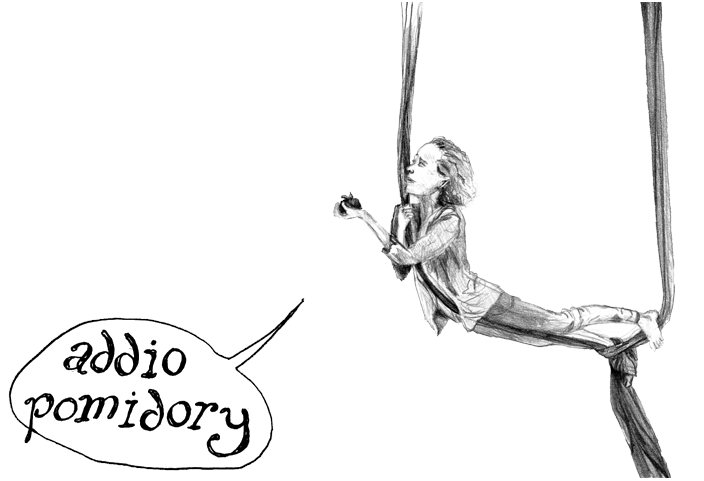
\includegraphics[height=0.6\textwidth]{images/addio_pomidory.png}\vspace*{-0.6\textwidth}
  \hspace*{5mm}(A!) \\
  \hspace*{5mm}(U!) \\
  \\
  Owszem, była i dziewczyna, i miłości pajęczyna\\
  Co oplotła drżący dwukwiat naszych ciał\\
  Porwał dziewczę zdrady poryw i zabrała pomidory\\
  Te ostatnie, com schowane przed nią miał\\
\end{minipage}
\begin{minipage}[t]{0.2\textwidth}
  a, d a\\
  d a E\\
  a, d G C\\
  d H$^7$ E\\

  a, d a\\
  d a d E\\
  a (A), d G C\\
  d a, d E a\\
  \\
  d$^7$ G$^7$ C A$^7$\\
  d G$^7$\\
  C (d) E$^7$\\
  \\
  a, d a\\
  Fis a, H$^7$ E$^7$ a\\
  d a E a\\
  d a E$^7$ a\\

  a, d a\\
  d a E\\
  a, d G C\\
  d H$^7$ E\\
\end{minipage}

\newpage
\section{Ain't no sunshine}\textcolor{lightgray}{\textit{Bill Withers}}\\~\\
\begin{minipage}[t]{0.8\textwidth}
  Ain't no sunshine when she's gone\\
  It's not warm when she's away\\
  Ain't no sunshine when she's gone\\
  And she's always gone too long, anytime she goes away\\
  \\
  Wonder this time where she's gone\\
  Wonder if she's gone to stay\\
  Ain't no sunshine when she's gone\\
  And this house just ain't no home, anytime she goes away\\
  \\
  \hspace*{5mm}And I know, I know, I know… ($\times$26)\\
  \hspace*{5mm}Hey, I ought to leave that young thing alone\\
  \hspace*{5mm}But ain't no sunshine when she's gone\\
  \\
  Ain't no sunshine when she's gone, only darkness everyday\\
  Ain't no sunshine when she's gone\\
  And this house just ain't no home, anytime she goes away\\
  Anytime she goes away
\end{minipage}
\begin{minipage}[t]{0.2\textwidth}
  a e G  a\\
  a e G  a\\
  a G  \\
  G d, F G a\\
  a e G  a\\

\end{minipage}

% \newpage
\section{Ale to już było}\textcolor{lightgray}{\textit{Maryla Rodowicz}}\\~\\
\begin{minipage}[t]{0.8\textwidth}
  Z wielu pieców się jadło chleb, bo od lat przyglądam się światu\\
  Nieraz rano zabolał łeb i mówili: zmiana klimatu\\
  Czasem trafił się wielki raut albo feta proletariatu\\
  Czasem podróż w najlepszym z aut, częściej szare drogi powiatu\\

  \hspace*{2mm} Ale to już było i nie wróci więcej\\
  \hspace*{2mm} I choć tyle się zdarzyło\\
  \hspace*{2mm} To do przodu wciąż wyrywa głupie serce\\
  \hspace*{2mm} Ale to już było znikło, gdzieś za nami\\
  \hspace*{2mm} Choć w papierach lat przebyło\\
  \hspace*{2mm} To naprawdę wciąż jesteśmy tacy sami\\

  Na regale kolekcja płyt i wywiadów pełne gazety\\
  Za oknami kolejny świt i w sypialni dzieci oddechy\\
  One lecą drogą do gwiazd przez niebieski ocean nieba\\
  Ale przecież za jakiś czas będą mogły same zaśpiewać\\

\end{minipage}
\begin{minipage}[t]{0.2\textwidth}

  C G C d G\\
  C G C d G\\
  e d F G \\
  e d F G \\

  F G C\\
  e\\
  F C \\
  F G C\\
  e\\
  F C \\

  C G C d G\\
  C G C d G\\
  e d F G \\
  e d F G \\

\end{minipage}

\newpage
\section{Aleksander Siergiejewicz Puszkin}\textcolor{lightgray}{\textit{Bułat Okudżawa}}\\~\\
\begin{minipage}[t]{0.8\textwidth}
  Co było nie wróci i szaty rozdzierać by próżno\\
  Cóż każda epoka ma własny porządek i ład\\
  A przecież mi żal że tu w drzwiach nie pojawi się puszkin\\
  Tak chętnie bym dziś choć na kwadrans na koniak z nim wpadł\\
  \\
  Dziś już nie musimy piechotą się wlec na spotkanie\\
  I tyle jest aut i rakiety unoszą nas w dal\\
  A przecież mi żal że po moskwie nie suną już sanie\\
  I nie ma już sań i nie będzie już nigdy a żal\\
  \\
  Przyjmuję pojętny mój wiek mego stwórcę i mistrza\\
  Ten trzeźwy mój wiek doświadczony mój wiek pragnę czcić\\
  A przecież mi żal że jak dawniej śnią nam się bożyszcza\\
  I jakoś tak jest że gotowiśmy czołem im bić\\
  \\
  No cóż nie na darmo zwycięstwem nasz wiek się uświetnił\\
  I wszystko już jest cicha przystań non iron i wikt\\
  A przecież mi żal że nad naszym zwycięstwem niejednym\\
  Górują cokoły na których nie stoi już nikt\\
  \\
  Co było nie wróci; wychodzę wieczorem na spacer\\
  I nagle spojrzałem na arbat i ach co za gość\\
  Rżą konie u sań Aleksander Siergiejewicz przechadza się\\
  Ach głowę bym dał że już jutro wydarzy się coś\\
\end{minipage}
\begin{minipage}[t]{0.2\textwidth}
  (a E)\\
  C G C A$^7$\\
  d G C a\\
  d E$^7$ a (A$^7$)\\

  d E a\\
  C G C A$^7$\\
  d G C a\\
  d E$^7$ a (A$^7$)\\

  d E a\\
  C G C A$^7$\\
  d G C a\\
  d E$^7$ a (A$^7$)\\

  d E a\\
  C G C A$^7$\\
  d G C a\\
  d E$^7$ a (A$^7$)\\

  d E a\\
  C G C A$^7$\\
  d G C a\\
  d E$^7$ a (A$^7$)\\
\end{minipage}

\newpage
\section{All about that bass}\textcolor{lightgray}{\textit{Meghan Trainor}}\\
\begin{minipage}[t]{0.8\textwidth}
  ~\\ 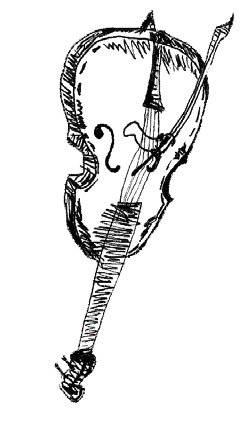
\includegraphics[height=4cm, angle=180, right]{images/all_about_that_bass_1.png}\vspace*{-4.3cm}
  \hspace*{5mm}Because you know\\
  \hspace*{5mm}I'm all about that bass\\
  \hspace*{5mm}'Bout that bass, no treble \hspace*{15mm}$\times$4\\

  Yeah, it's pretty clear, I ain't no size two\\
  But I can shake it, shake it, like I'm supposed to do\\
  'Cause I got that boom boom that all the boys chase\\
  And all the right junk in all the right places\\
  \\
  I see the magazine workin' that Photoshop\\
  We know that shit ain't real, come on now, make it stop\\
  If you got beauty, beauty, just raise 'em up\\
  'Cause every inch of you is perfect from the bottom to the top\\

  \hspace*{3mm}Yeah, my mama she told me Don't worry about your size\\
  \hspace*{3mm}She says, Boys like a little more booty to hold at night\\
  \hspace*{3mm}You know I won't be no stick figure silicone Barbie doll\\
  \hspace*{3mm}So if that's what you're into, then go 'head and move along\\
  \\
  I'm bringing booty back! Go 'head and tell them\\
  Skinny bitches that… No, I'm just playing\\
  I know you think you're fat, but I'm here to tell ya...\\
  Every inch of you is perfect from the bottom to the top\\
\end{minipage}
\begin{minipage}[t]{0.2\textwidth}
  ~\\
  (A h E A)\\~\\~\\~\\
  A\\
  h\\
  E\\
  A\\

  A\\
  h\\
  E\\
  A\\

  A h\\
  E A (E)\\
  A h\\
  E A\\

  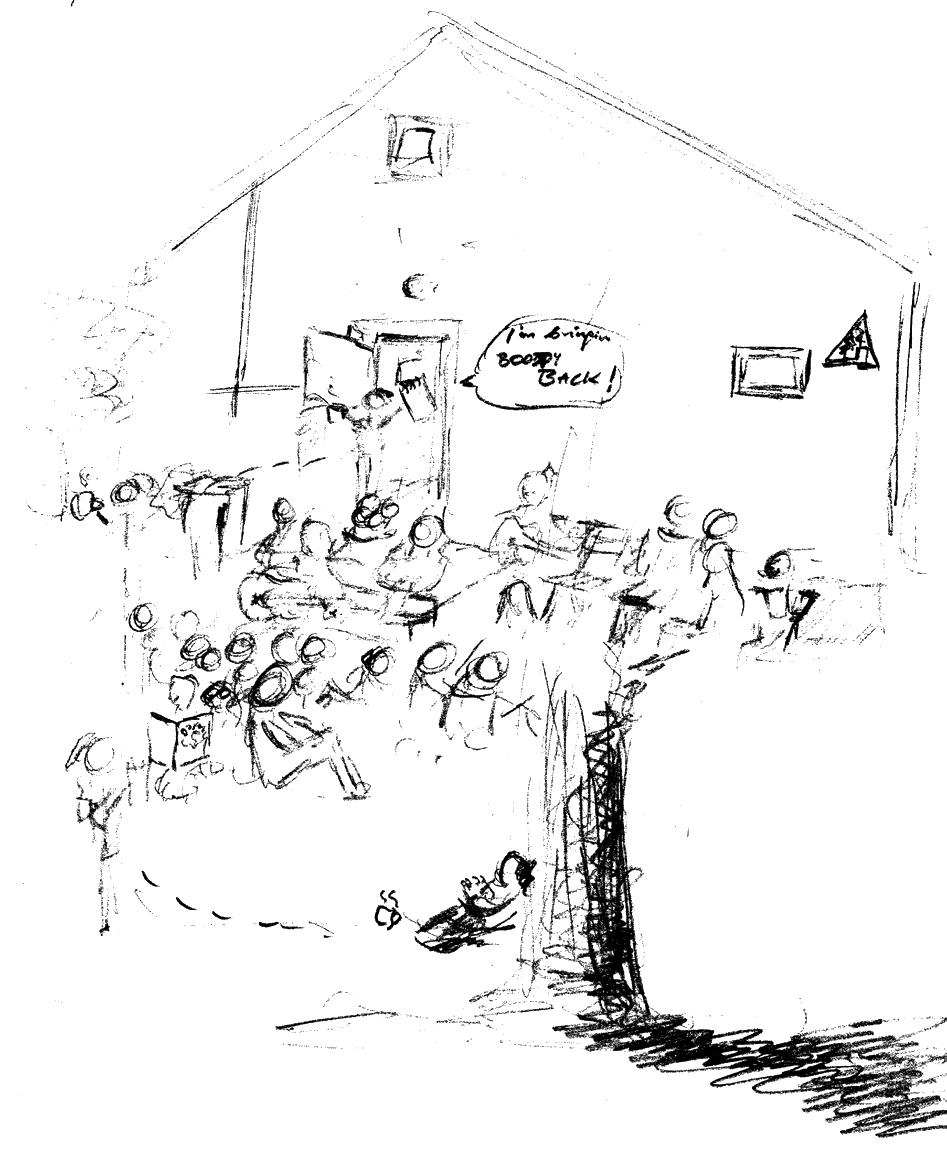
\includegraphics[height=10cm, right]{images/all_about_that_bass_2.png}\vspace*{-10cm}\\
  A\\
  h\\
  E\\
  A\\
\end{minipage}

\newpage
\section{Always on my mind}\textcolor{lightgray}{\textit{Elvis Presley}}\\~\\
\begin{minipage}[t]{0.8\textwidth}
  Maybe I didn't treat you\\
  Quite as good as I should\\
  Maybe I didn't love you\\
  Quite as often as I could\\
  \\
  \hspace*{4mm}Little things I should have said and done\\
  \hspace*{4mm}I never took the time\\
  \hspace*{4mm}You were always on my mind\\
  \hspace*{4mm}You were always on my mind\\
  \\
  Maybe I didn't hold you\\
  All those lonely, lonely times\\
  And I guess I never told you\\
  I am so happy that you're mine\\
  \\
  \hspace*{4mm}If I made you feel second best\\
  \hspace*{4mm}I'm so sorry I was blind\\
  \hspace*{4mm}You were always on my mind\\
  \hspace*{4mm}You were always on my mind\\
  \\
  \hspace*{8mm}Tell me,\\
  \hspace*{8mm}Tell me that your sweet love hasn't died\\
  \hspace*{8mm}Give me,\\
  \hspace*{8mm}One more chance to keep you satisfied\\
  \hspace*{8mm}Satisfied\\
  \\
  \hspace*{4mm}Little things...\\
\end{minipage}
\begin{minipage}[t]{0.2\textwidth}
  G D\\
  eD C (D)\\
  G D\\
  eD A\\

  C G\\
  C G a\\
  D G\\
  CD G (CD)\\

  G D\\
  eD C (D)\\
  G D\\
  eD A\\

  C G\\
  C G a\\
  D G\\
  CD G (CD)\\

  G D e D\\
  C G a D\\
  G D e D\\
  C G a$^7$ D\\
  G\\
\end{minipage}

\newpage
\section{Angie }\textcolor{lightgray}{\textit{The Rolling Stones}}\\~\\
\begin{minipage}[t]{0.8\textwidth}
  ~ \\
  Angie, Angie - When will those clouds all disappear\\
  Angie, Angie - Where will it lead us from here\\

  \hspace*{2mm} With no lovin' in our souls and no money in our coats\\
  \hspace*{2mm} You can't say we're satisfied\\

  Angie, Angie - You can't say we never tried\\

  Angie, you're beautiful, but ain't it time we say goodbye?\\
  Angie, I still love you, remember all those nights we cried\\

  \hspace*{2mm} All the dreams were held so close seemed to all go up in smoke\\
  \hspace*{2mm} Let me whisper in your ear\\

  Angie, Angie - Where will it lead us from here\\

  \hspace*{2mm} Oh, Angie, don't you wish, oh, your kisses still taste sweet\\
  \hspace*{2mm} I hate that sadness in your eyes\\

  But Angie, Angie - Ain't it time we say goodbye?\\

  \hspace*{2mm} With no lovin' in our souls and no money in our coats\\
  \hspace*{2mm} You can't say we're satisfied\\

  \hspace*{3mm} Angie, I still love you baby\\
  \hspace*{3mm} Everywhere I look I see your eyes\\
  \hspace*{3mm} There ain't a woman that comes close to you\\
  \hspace*{3mm} Come on baby dry your eyes\\

  Angie, Angie - Ain't it good to be alive\\
  Angie, Angie - We can't say we never tried\\

\end{minipage}
\begin{minipage}[t]{0.2\textwidth}
  a E$^7$, G F C \\
  a E$^7$, G F C \\
  a E$^7$, G F C \\

  G d a\\
  C F G\\

  a E$^7$,  G F C \\

  a E$^7$,  G F C \\
  a E$^7$,  G F C \\

  G d a\\
  C F G\\

  a E$^7$, G F C \\

  G d a\\
  C F G\\

  a E$^7$, G F C \\

  G d a\\
  C F G\\

  d a\\
  d a\\
  d a\\
  C F G\\

  a E$^7$, G F C \\
  a E$^7$, G F C \\

\end{minipage}

\newpage
\section{Baleron}\textcolor{lightgray}{\textit{}}\\~\\
\begin{minipage}[t]{0.8\textwidth}
  W pewnym małym miasteczku, gdzieś na krańcach Albanii\\
  Stary rzeźnik Alberto miał sklep mięsny z mięsami\\
  I czy pan był bogaty, pan był biedny, czy cieć\\
  Każdy dobry baleron chciał żreć\\

  \hspace*{8mm}Ten baleron dla zgłodniałych cavaleros\\
  \hspace*{8mm}Z baleronem będziesz senior prezentował się jak struś\\
  \hspace*{8mm}Na baleron i kiełbasę ty się skuś\\

  Jaki chcesz pan baleron, biały, czarny, czerwony\\
  Zakrapiany tymiankiem, czy też mocno pieprzony\\
  Jaki chcesz pan baleron, dużo tłuszczu, czy nie\\
  Jaki chcesz pan baleron? Ole!\\
  \\
  Na corridę, gdy pójdziesz z baleronem ukrytym\\
  Wtedy mocniej zabije serce twej seniority\\
  I gdy ona zemdlona na twe łono bez sił\\
  Padnie, szepcząc: Amigo! Gdzieś go skrył?\\
\end{minipage}
\begin{minipage}[t]{0.2\textwidth}
  a G\\
  F E\\
  a G\\
  F E\\

  a G \\
  F E F E\\
  F E \\

  a G\\
  F E\\
  a G\\
  F E\\

  a G\\
  F E\\
  a G\\
  F E\\
\end{minipage}

\newpage
\section{Ballada o Felku Zdankiewiczu}\textcolor{lightgray}{\textit{Stanisław Grzesiuk}}\\~\\
\begin{minipage}[t]{0.8\textwidth}
  Felek Zdankiewicz był chłopak morowy\\
  Przyjechał na urlop sześciotygodniowy\vspace*{2.2mm}\\
  \hspace*{5mm}Ojra, tarira ojra, tarira ojra, tarira, raz, dwa, trzy!\vspace*{2.2mm}\\
  Urlop się kończy, czas do wojska wrócić\\
  Ale Felusiowi żal koleżków rzucić\vspace*{1.8mm}\\
  Nie tak koleżków, jak swojej kochanki\\
  U której przebywał wieczory i ranki\vspace*{1.8mm}\\
  Wreszcie go schwytali grudnia trzynastego\\
  I zawieźli jego do biura śledczego\vspace*{1.8mm}\\
  A z biura śledczego wypuścić nie chcieli\\
  Felka Zdankiewicza na kluczyk zamknęli\vspace*{1.8mm}\\
  Lecz Feluś nie gapa, już nożyk otwiera\\
  Przebił Czajkowskiego, na Fuksa naciera\vspace*{1.8mm}\\
  Ledwie wyskoczył za bramę ratusza\\
  Wsiada do dorożki, na Warszawę rusza\vspace*{1.8mm}\\
  A w tej dorożce miał czasu troszkie\\
  Więc kazał się zawieźć aż na Czerniakowskie\vspace*{1.8mm}\\
  A z Czerniakowskiej do domu swojego\\
  Żeby opowiedzieć Mańce coś nowego\vspace*{1.8mm}\\
  Połóż się Feluś, boś ty jest pijany\\
  Połóż się Feluś, boś ty niewyspany\vspace*{1.8mm}\\
  Kładzie się Feluś do snu kamiennego\\
  A kochanka jego do biura śledczego\vspace*{1.8mm}\\
  Panowie agenci, prędko pospieszajcie\\
  Felka Zdankiewicza na łóżku schwytajcie\vspace*{1.8mm}\\
  Panowie agenci prędko pospieszyli\\
  Felka Zdankiewicza z nogami nakryli\vspace*{1.8mm}\\
  Jedzie kibitka wąską ulicą\\
  A koledzy jemu szczęścia, zdrowia życzą\vspace*{1.8mm}\\
  Ach wy koledzy, czyż wy nie żyjecie\\
  Czy wy mojej Mańce życie darujecie\vspace*{1.8mm}\\
  Nie martw się, Feluś, my jeszcze żyjemy\\
  I tę twoją Mańkę smykiem posuniemy\vspace*{1.8mm}\\
  Młoda Felusiowa już w grobie spoczywa\\
  A my na to konto gruchniem sobie piwa\vspace*{1.8mm}\\
\end{minipage}
\begin{minipage}[t]{0.4\textwidth}
  C G\\
  G$^7$ C C$^7$\vspace*{2.2mm}\\
  F C G C (G C)\vspace*{2.2mm}\\

\end{minipage}

\newpage
\section{Ballada o krzyżowcu}\textcolor{lightgray}{\textit{Mirosław Hrynkiewicz}}\\~\\
\begin{minipage}[t]{0.85\textwidth}
  Wolniej, wolniej, wstrzymaj konia, dokąd pędzisz, w stal odziany\\
  Pewnie tam, gdzie błyszczą w dali Jeruzalem białe ściany\\
  Pewnie myślisz, że w świątyni zniewolony Pan twój czeka\\
  Abyś przyszedł go ocalić, abyś przyszedł doń z daleka\\
  \\
  Wolniej, wolniej, wstrzymaj konia, byłem wczoraj w Jeruzalem\\
  Przemierzałem puste sale, Pana twego nie widziałem\\
  Pan opuścił Święte Miasto przed minutą, przed godziną\\
  W chłodnym gaju na pustyni z Mahometem piją wino\\
  \hspace*{10cm}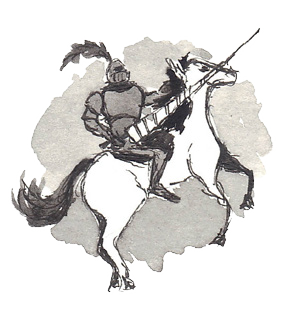
\includegraphics[height=3cm]{images/ballada_o_krzyzowcu.png}\vspace*{-3cm}\\

  Wolniej, wolniej, wstrzymaj konia, chcesz oblegać Jeruzalem\\
  Strzegą go wysokie wieże, strzegą go mahometanie\\
  Pan opuścił Święte Miasto, na nic poświęcenie twoje\\
  Po co niszczyć białe wieże, po co ludzi niepokoić\\
  \\
  Wolniej, wolniej, wstrzymaj konia, porzuć walkę niepotrzebną\\
  Porzuć miecz i włócznię swoją i jedź ze mną, i jedź ze mną\\
  Bo gdy szlakiem ku północy podążają hufce ludne\\
  Ja unoszę dumnie głowę i odjeżdżam na południe\\
\end{minipage}
\begin{minipage}[t]{0.2\textwidth}
  e A\\C D\\
\end{minipage}


\newpage
\section{Bandyta}\textcolor{lightgray}{\textit{Wojciech Brzeziński}}\\~\\
\begin{minipage}[t]{0.81\textwidth}
  Nie chciałem śpiewać ani pić i bez niej nie umiałem żyć\\
  To była miłość, szczenięca miłość\\
  \hspace*{5mm}  A jeden z tych, co mieli ją\\
  \hspace*{5mm}  Powiedział: Pędź, gówniarzu, won!\\
  \hspace*{5mm}  Powiedział: Pędź, gówniarzu, won! Aż mnie zmroziło!\\

  A jeden z tych, co mieli ją, ubliżał mi, wyzywał, klął\\
  Ja się w ten układ wpychać nie chciałem\\
  \hspace*{5mm}Lecz kiedy miałem spadać już\\
  \hspace*{5mm}Ona rzuciła krótko: Tchórz!\\
  \hspace*{5mm}Ona rzuciła krótko: Tchórz! Więc z nią zostałem\\

  A jeden z tych, co niech go szlag, podskoczył do mnie, krzycząc tak\\
  Chodź na solówkę, nie masz wyboru\\
  \hspace*{5mm}Wychodzę, mam być sam na sam\\
  \hspace*{5mm}Honor to święta rzecz, a tam\\
  \hspace*{5mm}Honor to święta rzecz, a tam ośmiu bandziorów\\

  Obcy mi cykor, bliski gniew, nie mdlałem nigdy widząc krew\\
  Nóż mieć w kieszeni zawsze wypada\\
  \hspace*{5mm}Trudno przewidzieć własny los\\
  \hspace*{5mm}Lecz pierwszy możesz zadać cios\\
  \hspace*{5mm}Lecz pierwszy możesz zadać cios - to jest zasada\\

  Gdy zazgrzytała stal o kość, myślałem: Będą mieli dość\\
  Mogłem się cofnąć, lecz mi odbiło\\
  \hspace*{5mm}Źle, gdy się człowiek głupio rwie\\
  \hspace*{5mm}Paru od tyłu zaszło mnie\\
  \hspace*{5mm}Paru od tyłu zaszło mnie, za późno było\\
\end{minipage}
\begin{minipage}[t]{0.19\textwidth}
  a\\
  d a\\
  d\\
  a\\
  E a (A$^7$)/(E a)\\

  a\\
  d a\\
  d\\
  a\\
  E a (A$^7$)/(E a)\\

  a\\
  d a\\
  d\\
  a\\
  E a (A$^7$)/(E a)\\

  a\\
  d a\\
  d\\
  a\\
  E a (A$^7$)/(E a)\\

  a\\
  d a\\
  d\\
  a\\
  E a (A$^7$)/(E a)\\

\end{minipage}
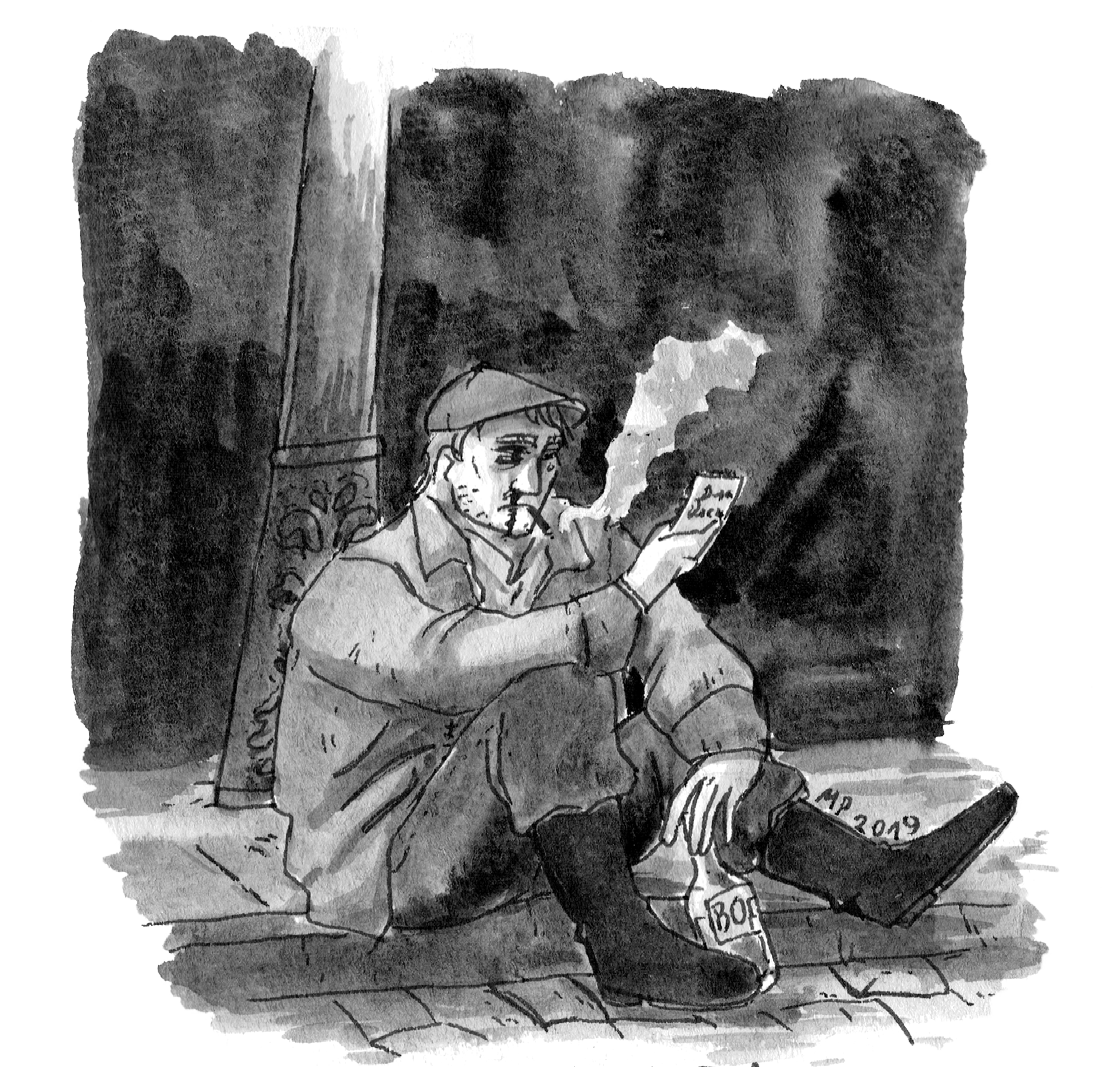
\includegraphics[height=5.5cm,center]{images/bandyta.png}
\newpage
\begin{minipage}[t]{0.8\textwidth}
  Pan prokurator z ran mych drwi, zamknęły się więzienia drzwi\\
  Tam, w lazarecie, dogorywałem\\
  \hspace*{5mm}Felczer na żywo rany szył\\
  \hspace*{5mm}I mówił: Będziesz, brachu, żył!\\
  \hspace*{5mm}I mówił: Będziesz, brachu, żył! A ja żyć chciałem\\

  Odsiedzę, co odsiedzieć mam, ona nie przyjdzie, głowę dam\\
  Ja jej nie winię, wcale nie winię\\
  \hspace*{5mm}Żyję pod konstelacją złą,\\
  \hspace*{5mm}Lecz jeden z tych, co mieli ją\\
  \hspace*{5mm}Lecz jeden z tych, co mieli ją, na pewno /już wkrótce/ zginie\\
\end{minipage}
\begin{minipage}[t]{0.2\textwidth}
  a\\
  d a\\
  d\\
  a\\
  E a (A$^7$)/(E a)\\

  a\\
  d a\\
  d\\
  a\\
  E a (A$^7$)/(E a)\\
\end{minipage}
\vspace*{2cm}\\
---\hfill\textcolor{lightgray}{\textit{Dawid Ignasiak, VII 2018}}\\~\\
\begin{minipage}[b]{0.8\textwidth}
  Nie chciałem butów ściągać już, myślałem: schronisko tuż tuż\\
  Mnie się spieszyło, strasznie spieszyło		\\
  \hspace*{5mm}Lecz kiedy woda wlała się				\\
  \hspace*{5mm}Zachlupotała mi w bucie!					\\
  \hspace*{5mm}Zachlupotała mi w bucie! Aż mnie zmroziło!\\
  \\
  Gdy mi tak przemókł lewy but, to Szef pokazał jakiś skrót\\
  Uraczył wszystkich jeszcze godziną\\
  \hspace*{5mm}Źle gdy się człowiek głupio rwie\\
  \hspace*{5mm}Pęcherze hurtem tworzą się\\
  \hspace*{5mm}Pęcherze hurtem tworzą się - będzie krwawiło\\
  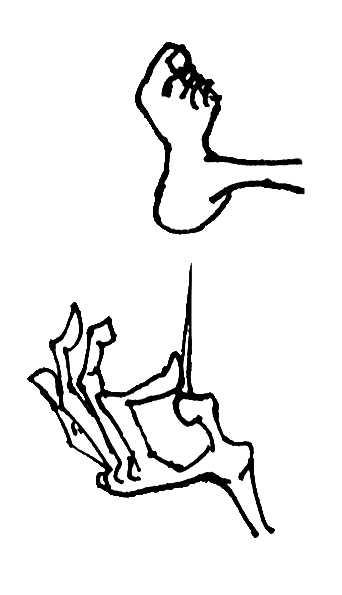
\includegraphics[height=2.5cm,right]{images/stopa_dejwa.png}\vspace*{-2.6cm}\\

  Cała ekipa z ran mych drwi, zamknęły się namiotu drzwi\\
  Na kanadyjce dogorywałem\\
  \hspace*{5mm}Grzesiu na żywo stopy kłuł\\
  \hspace*{5mm}I mówił: Nic nie będziesz czuł!\\
  \hspace*{5mm}I mówił: Nic nie będziesz czuł! A ja płakałem\\
  \\
  Odczekam co odczekać mam do zagojenia wszystkich ran\\
  Dzisiaj me stopy ledwie unoszę\\
  \hspace*{5mm}Teraz odwozi mnie autobus\\
  \hspace*{5mm}Lecz na następny obóz\\
  \hspace*{5mm}Lecz na następny obóz wezmę kalosze /już się nie zgłoszę/\\
\end{minipage}
\begin{minipage}[b]{0.2\textwidth}
  a\\
  d a\\
  d\\
  a\\
  E a (A$^7$)/(E a)\\

  a\\
  d a\\
  d\\
  a\\
  E a (A$^7$)/(E a)\\

  a\\
  d a\\
  d\\
  a\\
  E a (A$^7$)/(E a)\\

  a\\
  d a\\
  d\\
  a\\
  E a (A$^7$)/(E a)\\
\end{minipage}

\newpage
\section{Baranek}\textcolor{lightgray}{\textit{KULT}}\\~\\
\begin{minipage}[t]{0.8\textwidth}
  Ach Ci ludzie, to brudne świnie\\
  Co napletli o mojej dziewczynie\\
  Jakieś bzdury o jej nałogach\\
  To po prostu litość i trwoga\\
  Tak to bywa gdy ktoś zazdrości\\
  Kiedy brak mu własnej miłości\\
  Plotki płodzi, mnie nie zaszkodzi żadne obce zło\\
  Na mój sposób widzieć ją\\

  \hspace*{5mm}Na głowie kwietny ma wianek\\
  \hspace*{5mm}W ręku zielony badylek\\
  \hspace*{5mm}A przed nią bieży baranek\\
  \hspace*{5mm}A nad nią lata motylek\\

  Krzywdę robią mojej panience\\
  Opluć chcą ją podli zboczeńcy\\
  Utopić chcą ją w morzu zawiści\\
  Paranoicy, podli sadyści\\
  Utaplani w brudnej rozpuście\\
  A na gębach fałszywy uśmiech\\
  Byle zagnać do swego bagna, ale wara wam\\
  Ja ją przecież lepiej znam\\

  Znów widzieli ją z jakimś chłopem\\
  Znów wyjechała do St. Tropez\\
  Znów męczyła się, Boże drogi\\
  Znów na jachtach myła podłogi\\
  Tylko czemu ręce ma białe\\
  Chciałem zapytać, zapomniałem\\
  Ciało kłoniąc skinęła dłonią wsparła skroń o skroń\\
  Znów zapadłem w nią jak w toń\\

  Ech, dziewczyna pięknie się stara\\
  Kosi pieniądz, ma jaguara\\
  Trudno pracę z miłością zgodzić\\
  Rzadziej może do mnie przychodzić\\
  Tylko pyta kryjąc rumieniec\\
  Czemu patrzę jak potępieniec\\
  Czemu zgrzytam, kiedy się pyta czy ma ładny biust\\
  Czemu toczę pianę z ust\\
\end{minipage}
\begin{minipage}[t]{0.2\textwidth}
  A\\
  d\\
  A\\
  d\\
  D\\
  g\\
  A d\\
  A d\\

  A d\\
  A d\\
  g D\\
  A d\\

  A\\
  d\\
  A\\
  d\\
  D\\
  g\\
  A d\\
  A d\\

  A\\
  d\\
  A\\
  d\\
  D\\
  g\\
  A d\\
  A d\\

  A\\
  d\\
  A\\
  d\\
  D\\
  g\\
  A d\\
  A d\\

\end{minipage}

\newpage
\section{Bardzo smutna piosenka retro}\textcolor{lightgray}{\textit{Pod Budą}}\\~\\
\begin{minipage}[t]{0.8\textwidth}
  Lato było jakieś szare i słowikom brakło tchu\\
  Smutnych wierszy parę ktoś napisał znów\\
  Smutnych wierszy nigdy dosyć, i zranionych ciężko serc\\
  Nieprzespanych nocy, które trawi lęk\\
  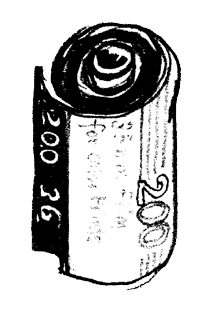
\includegraphics[height=3cm,right]{images/bardzo_smutna_piosenka.png}\vspace*{-31mm}\\
  \\
  \hspace*{5mm}Kap, kap, płyną łzy, w łez kałużach ja i ty\\
  \hspace*{5mm}Wypłakane oczy i przekwitłe bzy\\
  \hspace*{5mm}Płacze z nami deszcz i fontanna szlocha też\\
  \hspace*{5mm}Trochę zadziwiona, skąd ma tyle łez\\
  \\
  Nad dachami muza leci, muza czyli weny znak\\
  Czemuż wam, poeci, miodu w sercach brak\\
  Muza ma sukienkę krótką, muza skrzydła ma u rąk\\
  Lecz wam ciągle smutno, a mnie boli ząb\\
\end{minipage}
\begin{minipage}[t]{0.2\textwidth}
  C G$^7$ C G$^7$\\
  E$^7$ a D$^7$ G$^7$\\
  C G$^7$ C G$^7$\\
  E$^7$ a D$^7$ G$^7$\\
  \\
  C G$^7$ C G$^7$\\
  C A$^7$ d G C (G C)\\
  C G$^7$ C G$^7$\\
  C A$^7$ d G C (G C)\\
  \\
  C G$^7$ C G$^7$\\
  E$^7$ a D$^7$ G$^7$\\
  C G$^7$ C G$^7$\\
  E$^7$ a D$^7$ G$^7$\\
\end{minipage}

% \newpage
\section{Beskid}\textcolor{lightgray}{\textit{Andrzej Wierzbicki}}\\~\\
\begin{minipage}[t]{0.78\textwidth}
  A w Beskidzie rozzłocony buk			\\
  A w Beskidzie rozzłocony buk 				\\
  Bedę chodził Bukowiną z dłutem w ręku			\\
  By w dziewczęcych twarzach		\\
  Uśmiech rzeźbić, niech nie płaczą już		\\
  Niech się cieszą po kapliczkach moich dróg\\
  \\
  \hspace*{4mm}W Beskidzie malowany cerkiewny dach 			\\
  \hspace*{4mm}W Beskidzie zapach miodu w bukowych pniach 		\\
  \hspace*{4mm}Tutaj wracam, gdy ruda jesień na przełęcze swój toboł niesie\\
  \hspace*{4mm}Słucham bicia dzwonów w przedwieczorny czas 		\\
  \\
  \hspace*{4mm}W Beskidzie malowany wiatrami dom\\
  \hspace*{4mm}W Beskidzie - tutaj słowa inaczej brzmią\\
  \hspace*{4mm}Kiedy krzyczę w jesienną ciszę, kiedy wiatrem szeleszczą liście\\
  \hspace*{4mm}Kiedy wolność się tuli w ciepło moich rąk\\
  \hspace*{4mm}Gdy jak źrebak się tuli do mych rąk\\
  \\
  A w Beskidzie zamyślony czas\\
  A w Beskidzie zamyślony czas\\
  Bedę chodził z nim poddaszem gór\\
  By zerwanych marzeń struny\\
  Przywiązywać niespokojnym dłoniom drzew\\
  Niech mi grają na rozstajach moich dróg\\
\end{minipage}
\begin{minipage}[t]{0.22\textwidth}
  G C D G C D\\
  G C a$^7$ D\\
  C D G\\
  G C\\
  G C a$^7$ D\\
  C D G C D\\
  \\
  G C D G\\
  G C H$^7$ e\\
  C D G C\\
  G C a$^7$ D\\

  G C D G\\
  G C H$^7$ e\\
  C D G C\\
  G C a$^7$ D\\
  C D G\\
  \\
  G C D G C D\\
  G C a$^7$ D\\
  C D G\\
  G C\\
  G C a$^7$ D\\
  C D G C D\\
\end{minipage}

\newpage
\section{Beskidzkie country}\textcolor{lightgray}{\textit{Janusz Witkowski, Jakub Jugo; VII 2019}}\\~\\
\begin{minipage}[t]{0.8\textwidth}
  Lipcowe słońce wschodzi, czuć w wietrze zapach mięty\\
  Wszystkich ochota nachodzi, by zniszczyć sobie pięty \\
  Szef w poście info daje, ku uciesze i przestrodze\\
  Że w Beskidzie zawitajem, lecz cenowo nie po drodze\vspace*{2mm}
  \\
  \hspace*{5mm}Obóz za tysiąc złotych, jedyne tysiąc ziko x2\vspace*{2mm}
  \\
  Choć cena nie gra roli, to trzepie po portfelu\\
  Wszystkie kieszenie boli, przeszkodą jest dla wielu \\
  Niektóre dzbany zresztą, dojeżdżają w tydzień drugi\\
  Janusz, Tymon, Karol z Jeszką, ale mistrzem w tym jest Dżogi \vspace*{2mm}
  \\
  \hspace*{5mm}Pojawia się i znika, taki już los muzyka\\
  \hspace*{5mm}Pojawia się i znika, Dżogi uruchamia Krzycha\vspace*{2mm}
  \\
  A jak Dżogi to też kostki, ścięgna, stawy kolanowe\\
  Z drobiu, takie z szczyptą chrząstki, lepsze jednak obrotowe \\
  Więc teraz tu dla państwa, lejdis, panie i panowie\\
  Piękny i wspaniały Dawid złoży kostkę, ja wam powiem! \vspace*{2mm}
  \\
  {\small \textit{[kostka, bridge]}}\vspace*{2mm}
  \\
  \hspace*{5mm}Cóż to za szybki dzik, zero piętnaście w mig $\times$ 2\vspace*{2mm}
  \\
  Każdego dnia łazimy, ciągnąc kilometry z szosy\\
  Może więcej zrobimy, jedząc zwykłe kabanosy \\
  Ostatni nasz przystanek, na Niemcowej w domu wielkim\\
  Lecz nie sposób wejść na ganek, bo zajęły go harcerki \vspace*{2mm}
  \\
  \hspace*{5mm}Harcerki wzięły wodę i wymyć się nie mogę $\times$ 2\vspace*{2mm}
  \\
  Dlatego macie bana, trza coś zrobić z naczyniami\\
  Ale w zamian można z rana, zająć się otrzęsinami \\
  Najlepsze że Wam piszą, piosenkę obozową\\
  Same wafle co wyjazdu, cieszą się ledwie połową \vspace*{2mm}
  \\
  {\small \textit{[bridge]}} \vspace*{2mm}
  \\
  \hspace*{5mm}Obóz za tysiąc złotych, jedyne tysiąc ziko\\
  \hspace*{5mm}Mogliśmy złapać stopa i byłoby za friko \vspace*{2mm}
  \\
  \hspace*{10mm}Czerwononosy Olek, namiot nieposkładany\\
  \hspace*{10mm}Zamknięta Radziejowa, a Szefu niewyspany\\
  \hspace*{2cm}$\times \infty $

\end{minipage}
\begin{minipage}[t]{0.2\textwidth}
\end{minipage}

\newpage
\section{Bez słów}\textcolor{lightgray}{\textit{WGB}}\\~\\
\begin{minipage}[t]{0.85\textwidth}
  Chodzą ulicami ludzie, maj przechodzą, lipiec, grudzień\\
  Zagubieni wśród ulic, bram\\
  Przemarznięte grzeją dłonie, dokądś pędzą, za czymś gonią\\
  I budują wciąż domki z kart\\
  \\
  \hspace*{5mm}A tam w mech odziany kamień, tam zaduma w wiatru graniu\\
  \hspace*{5mm}Tam powietrze ma inny smak\\
  \hspace*{5mm}Porzuć kroków rytm na bruku, spróbuj - znajdziesz jeśli szukać\\
  \hspace*{5mm}Zechcesz - nowy świat, własny świat\\
  \\
  Płyną ludzie miastem, szarzy, pozbawieni złudzeń, marzeń\\
  Omijają wciąż główny nurt\\
  Kryją się w swych norach krecich i śnić nawet o karecie\\
  Co lśni złotem, nie potrafią już\\
  \\
  Żyją ludzie, asfalt depczą, nikt nie krzyknie, każdy szepcze\\
  Drzwi zamknięte, zaklepany krąg\\
  Tylko czasem kropla z oczu po policzku w dół się stoczy\\
  I to dziwne drżenie rąk\\
\end{minipage}
\begin{minipage}[t]{0.2\textwidth}
  G D e h\\
  C G D\\
  G D e h\\
  C G D\\

  C G C G\\
  C G D\\
  C G C G\\
  C G D\\

  G D e h\\
  C G D\\
  G D e h\\
  C G D\\

  G D e h\\
  C G D\\
  G D e h\\
  C G D\\
\end{minipage}

\newpage
\section{Biały miś}\textcolor{lightgray}{\textit{Jan Tarka / Badyle}}\\~\\
\begin{minipage}[t]{0.7\textwidth}
  Biały miś, dla dziewczyny\\
  Którą kocham i kochał będę wciąż\\
  Lecz dziewczyna jest już z innym\\
  Dziś pozostał mi po niej smutek, żal\\

  \hspace*{4mm} Hej dziewczyno, spójrz na misia\\
  \hspace*{4mm} On przypomni, przypomni chłopca ci\\
  \hspace*{4mm} Nieszczęśliwego, białego misia\\
  \hspace*{4mm} Który w oczach ma tylko szare łzy\\

  Płynie czas, tak jak rzeka\\
  I nie wrócą, nie wrócą tamte dni\\
  W moim sercu jest dziś rana\\
  Którą zatrzeć możesz tylko ty\\

\end{minipage}
\begin{minipage}[t]{0.3\textwidth}
  a d\\
  F G a E\\
  a d\\
  F G a G\\

  C d\\
  F G a G\\
  C d\\
  F G a E\\

  a d\\
  F G a E\\
  a d\\
  F G a G\\

\end{minipage}

% \newpage
\section{Bieszczady}\textcolor{lightgray}{\textit{Adam Chmiel}}\\~\\
\begin{minipage}[t]{0.7\textwidth}
  Tu w dolinach wstaje mgłą wilgotny dzień\\
  Szczyty ogniem płoną, stoki kryje cień			\\
  Mokre rosą trawy wypatrują dnia\\
  Ciepła, które pierwszy słońca promień da\\
  \\
  \hspace*{5mm}Cicho potok gada, gwarzy pośród skał			\\
  \hspace*{5mm}O tym deszczu co z chmury trochę wody dał\\
  \hspace*{5mm}Świerki zapatrzone w horyzontu kres\\
  \hspace*{5mm}Głowy pragną wysoko, jak najwyżej wznieść\\
  \\
  Tęczą kwiatów barwny połoniny łan\\
  Słońcem wypełniony jagodowy dzban\\
  Pachnie świeżym sianem pokos pysznych traw\\
  Owiec dzwoneczkami cisza niebu gra\\
  \\
  Serenadą świerszczy, kaskadami gwiazd\\
  Noc w zadumie kroczy, mroku ścieląc płaszcz\\
  Wielkim wozem księżyc rusza na swój szlak\\
  Pozłocistym sierpem gasi lampy dnia\\

\end{minipage}
\begin{minipage}[t]{0.3\textwidth}
  e a\\
  D G H$^7$\\
  e a\\
  D G H$^7$\\

  G C D G\\
  G C D G\\
  G C D G\\
  G C D G (H$^7$)\\

  e a\\
  D G H$^7$\\
  e a\\
  D G H$^7$\\

  e a\\
  D G H$^7$\\
  e a\\
  D G H$^7$\\
\end{minipage}

\newpage
\section{Bieszczadzki riff}\textcolor{lightgray}{\textit{Janusz Witkowski, Jakub Jugo, VII 2018 }}\\~\\
\begin{minipage}[t]{1\textwidth}
  Peleryny, kurtki, płaszcze - widzę tylko w tych Bieszczadach\hfill a\\
  Wszędzie błoto, wszędzie brudno, wszystko tonie w rzecznych madach\\
  Sam do końca nie wiem w sumie, ile dni już tak wędruję\\
  Chciałbym w końcu umyć rzeczy, ale mydła mi brakuje\\
  \hspace*{3mm}Kurtka na mnie się rozpuszcza, w wodzie prosto z nieba dziury\\
  \hspace*{3mm}Zimno, że aż zęby dzwonią, słońca nie ma - to przez chmury\\
  \hspace*{3mm}Jeśli kiedyś będę w domu, gwizdnę mamie suszareczkę\\
  \hspace*{3mm}Ale raczej już nie zdołam, bo deszcz robi ze mnie sieczkę\\
  \\
  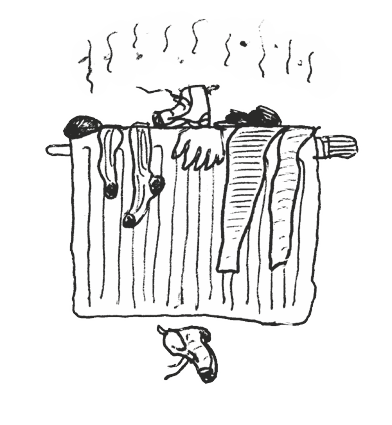
\includegraphics[height=0.3\textwidth, right]{images/bieszczadzki_riff_1.png}\vspace*{-0.3\textwidth}\\
  \hspace*{10mm}Ciągle pada - tylko w Bieszczadach $\times$4\\
  \hspace*{10mm}Jadę ($\times$6) w Bieszczady ziomy $\times$2\\

  Ropnie, bąble i odciski czuję tylko w tych Bieszczadach\\
  Cierpią stopy i kolana, nie pomaga czekolada\\
  Już nie jestem w stanie chodzić i w tej ściółce jeszcze brodzić\\
  Czeka na mnie amputacja, warto się z tym już pogodzić\\
  \hspace*{3mm}Pokój pełen tych śmierdzieli zmienia się w szpitalne skrzydło\\
  \hspace*{3mm}Przebijają se pęcherze, jak farmerzy znaczą bydło\\
  \hspace*{3mm}Kłuje ciebie łyda w nodze, jakby był tam jeżozwierz?\\
  \hspace*{3mm}Dam ci na to jedną radę: bierz Voltaren i się ciesz!\\
  \\
  \hspace*{10mm}Bąble z rana - tylko w Bieszczadach $\times$4\\
  \hspace*{10mm}Jadę ($\times$6) w Bieszczady ziomy $\times$2\\
  \\
  Kleszcze, muchy i komary słyszę tylko w tych Bieszczadach a\\
  Są ich setki lub tysiące - więcej matka ich nie miała\\
  Po co te cholerstwa żyją i dlaczego krew mi piją?\\
  W jakim celu Bóg je stworzył, czemu mi psychikę ryją?\\
  \hspace*{3mm}Siadam po dniu wędrowania, chociaż mam już z tym trudności\\
  \hspace*{3mm}Patrzę, widzę na mej nodze tuzin nieproszonych gości\\
  \hspace*{3mm}Zaraz wezmę w dłoń gazetę i w krwiopijców nią przyłożę\\
  \hspace*{3mm}A gdy skończę tę zabawę, buty sobie nią wyłożę\\

  \hspace*{10mm}Zgnieć owada - tylko w Bieszczadach $\times$4\\
  \hspace*{10mm}Jadę ($\times$6) w Bieszczady ziomy $\times$2\\

  \textit{(bridge)}\hfill d B $/ \times$3,
  F$^7$ E$^7$\\
\end{minipage}
\newpage
\begin{minipage}[t]{1\textwidth}
  ~\\
  Ale jedno przyznać muszę: że jest klawo w tych Bieszczadach\\
  Piękne szczyty i widoki, nocą gwiazdy na plejadach\\
  Pakuj plecak, idziem w góry, wynosimy się z tej dziury!\\
  Z wami wszędzie się zabiorę, towarzyskie me Wiewióry!\\
  \hspace*{3mm}Patrzę na ten gór ocean, płynąc grzbietem połoniny\\
  \hspace*{3mm}Niesłychaną słyszę ciszę, jedząc słodziutkie maliny\\
  \hspace*{3mm}Jak do tego dodać ludzi, co pomogą ci w potrzebie\\
  \hspace*{3mm}Możesz w snach się wnet zanurzyć, poczuć się jak w siódmym niebie\\
  \\
  \hspace*{10mm}Słuchaj rady - wyjedź w Bieszczady $\times$4\\
  \hspace*{10mm}Jadę ($\times$6) w Bieszczady ziomy $\times$2\\
  \\
  \\
  A teraz, panie i panowie, lejdis end dżentelmen\\
  Nasz piękny, wspaniały i niepowtarzalny\\
  \hspace*{4mm}\textit{\large WŁODZIMIERZ MIZIA}\\
  Zagra specjalnie dla państwa dżem seszyn\\
  W sensie solówkę\\
  Nie daj się prosić, Włodek\\
  Wszyscy wiemy, że tego bardzo pragniesz\\
  Dzisiejszy wieczór i panienki są Twoje!\\
  \\
  \\
  \\
  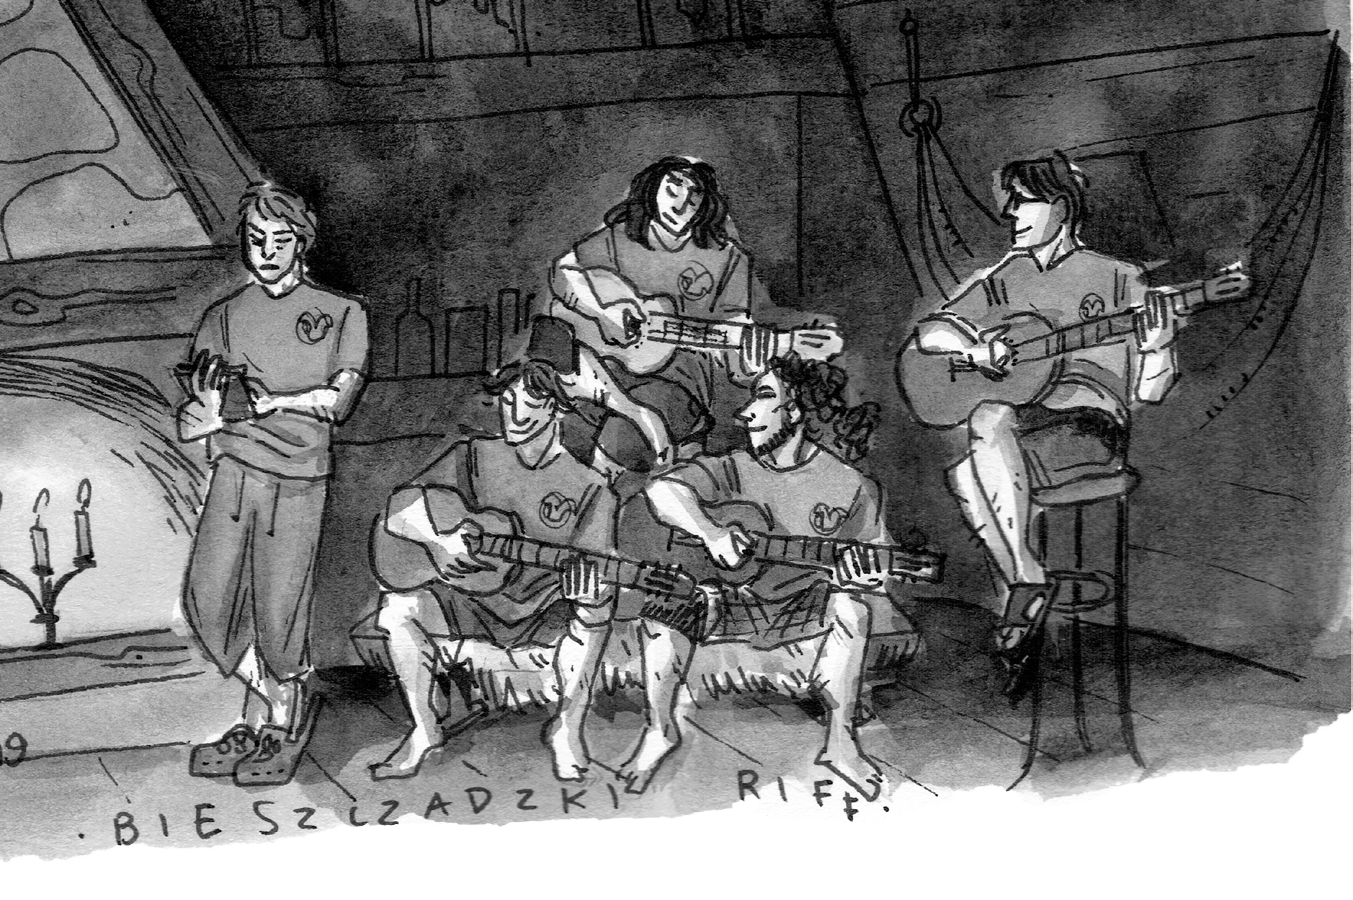
\includegraphics[width=12cm]{images/bieszczadzki_riff.png}
\end{minipage}

\newpage
\section{Bieszczadzkie anioły}\textcolor{lightgray}{\textit{SDM}}\\~\\
\begin{minipage}[t]{0.8\textwidth}
  Anioły są takie ciche, Zwłaszcza te w Bieszczadach\\
  Gdy spotkasz takiego w górach Wiele z nim nie pogadasz\\
  Najwyżej na ucho ci powie Gdy będzie w dobrym humorze\\
  Że skrzydła nosi w plecaku Nawet przy dobrej pogodzie\\
  \\
  Anioły są całe zielone Zwłaszcza te w Bieszczadach\\
  Łatwo w trawie się kryją I w opuszczonych sadach\\
  W zielone grają ukradkiem Nawet karty mają zielone\\
  Zielone mają pojęcie A nawet zielony kielonek\\
  \\
  \hspace*{4mm}Anioły bieszczadzkie bieszczadzkie anioły\\
  \hspace*{4mm}Dużo w Was radości i dobrej pogody\\
  \hspace*{4mm}Bieszczadzkie anioły anioły bieszczadzkie\\
  \hspace*{4mm}Gdy skrzydłem Cię dotkną już jesteś ich bratem\\
  \\
  Anioły są całkiem samotne Zwłaszcza te w Bieszczadach\\
  W kapliczkach zimą drzemią Choć może im nie wypada\\
  Czasem taki anioł samotny Zapomni dokąd ma lecieć\\
  I wtedy całe Bieszczady Mają szaloną uciechę\\
  \\
  Anioły są wiecznie ulotne Zwłaszcza te w Bieszczadach\\
  Nas też czasami nosi Po ich anielskich śladach\\
  One nam przyzwalają I skrzydłem wskazują drogę\\
  I wtedy w nas się zapala Wieczny bieszczadzki ogień\\
\end{minipage}
\begin{minipage}[t]{0.2\textwidth}
  a  G  \\
  a  e  \\
  C G  C F\\
  C G a e a\\

  a  G  \\
  a  e  \\
  C G  C F\\
  C G a e a\\

  C G a\\
  C G a\\
  C G a\\
  C G a\\

  a  G  \\
  a  e  \\
  C G  C F\\
  C G a e a\\

  a  G  \\
  a  e  \\
  C G  C F\\
  C G a e a\\
\end{minipage}


% \newpage
\section{Bieszczadzkie reggae}\textcolor{lightgray}{\textit{WBH}}\\~\\
\begin{minipage}[t]{0.6\textwidth}
  Porannej mgły snuje się dym\\
  Jutrzenki szal na stokach gór\\
  Nowy dzień budzi się, budzi się\\
  Melodię dnia już rosa gra\\

  \hspace*{5mm}Reggae, bieszczadzkie reggae\\
  \hspace*{5mm}Słońcem spalone, ma jagód smak\\
  \hspace*{5mm}Reggae, bieszczadzkie reggae\\
  \hspace*{5mm}Jak potok rwący przed siebie gna\\

  Połonin czar ma taką moc\\
  Że gdy je ujrzysz pierwszy raz\\
  Wrócić chcesz, wrócić chcesz znów za rok\\
  Z poranną rosą czekać dnia\\
\end{minipage}
\begin{minipage}[t]{0.4\textwidth}
  d C d C\\
  \\
  \\
  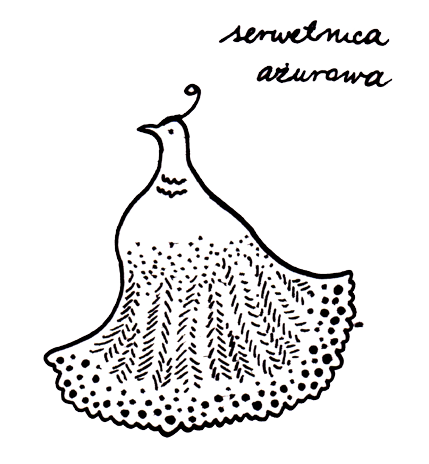
\includegraphics[width=0.8\textwidth]{images/bieszczadzkie_reggae.png}\\
\end{minipage}

\newpage
\section{Blues dla małej}\textcolor{lightgray}{\textit{SDM}}\\~\\
\begin{minipage}[t]{0.8\textwidth}
  Wystukaj po torach do mnie list\\
  Wtedy naprawdę nie wyjedziesz cała\\
  Niech będzie w nim lokomotywy gwizd\\
  Tylko to zrób jeszcze dla mnie, Mała\\
  Wystukaj po torach do mnie list\\
  Choćby w alfabecie Morse'a\\
  Moja ulica jeszcze twardo śpi\\
  Jeśli tak chcesz, w liście zostań\\
  \\
  % \includegraphics[height=0.35\textwidth, right]{images/blues_dla_małej.png}\vspace*{-0.353\textwidth}\\
  \hspace*{4mm} A mogliśmy, Mała, razem łąką iść\\
  \hspace*{4mm} Świt witać po kolana w rosie\\
  \hspace*{4mm} A mogliśmy, Mała, razem piwo pić\\
  \hspace*{4mm} Dom nasz zamienić na sto pociech\\
  \hspace*{4mm} A mogliśmy, Mała, konie kraść\\
  \hspace*{4mm} Z niebieskiego boskiego pastwiska\\
  \hspace*{4mm} A mogliśmy, Mała, w środku lata\\
  \hspace*{4mm} Zbudować słoneczną przystań\\

  Napisz od serca do mnie list\\
  I zamieszkaj w tym liście cała\\
  Niech śmiechu dużo będzie w nim\\
  Obiecaj mi to dzisiaj, Mała\\
  Napisz od serca do mnie list\\
  Lecz, proszę, nie wysyłaj go nigdy\\
  W szufladzie zamknij go na klucz\\
  Niech czeka wciąż lepszych dni\\
  \\
  \\
  \includegraphics[width=0.7\textwidth, right]{images/blues_dla_małej.png}\\
\end{minipage}
\begin{minipage}[t]{0.2\textwidth}
  C h$^{7-5}$\\
  a G\\
  F C\\
  h$^{7-5}$ E$^7$ a\\
  C h$^{7-5}$\\
  a G\\
  F C\\
  h$^{7-5}$ E$^7$ a\\

  h$^{7-5}$\\
  a\\
  G\\
  E\\
  F\\
  C\\
  h$^{7-5}$\\
  E a\\

  C h$^{7-5}$\\
  a G\\
  F C\\
  h$^{7-5}$ E$^7$ a\\
  C h$^{7-5}$\\
  a G\\
  F C\\
  h$^{7-5}$ E$^7$ a\\

  \chord{t}{n,p2,p3,p2,p3,n}{{\small h$^{7-5}$}}
\end{minipage}


\newpage
\section{Bo jak nie my to kto}\textcolor{lightgray}{\textit{Mrozu, Tomson}}\\~\\
\begin{minipage}[t]{0.8\textwidth}
  \hspace*{5mm}Bo jak nie my to kto? $\times 4$\\
  \hspace*{5mm}Bo jak nie my to nikt tego lepiej nie zrobi tu!\\

  Daj więcej beatu maestro, buja się całe sąsiedztwo\\
  Nie znamy granic i przez to potem czujemy się kiepsko\\
  Niedouczeni na błędach. Dzisiaj się tworzy legenda\\
  Za pomocą stopy i werbla. Dodaj do tego Amsterdam\\
  Wiesz dokładnie o co chodzi nam\\
  Bo ty chcesz osiągać idealny stan\\

  To są nasze najlepsze dni. Zaskakuję sam siebie i\\
  Potem z rana już nie wiem nic, ciągle mało jest jeszcze mi\\
  Moje życie bywa jak film, imprezuje jak Charlie Sheen\\
  Dynia pęka jak w Halloween, drina goni kolejny drin\\
  Wiesz dokładnie o co chodzi nam\\
  Bo ja też nocami odbijam się od ścian\\

  My lubimy jazz i lubimy chillout. Jaki ma sens się dziś spinać?\\
  Buzuje w nas ta endorfina, sukienka pin-up tak ciebie opina\\
  Ooo Błędny wzrok kolejny shot, łapię trop\\
  Brzdęk, brzdęk znika lęk, dzisiaj w klubie będzie bang!\\
  Jak ja dobrze to znam\\
  Grzeszne spojrzenia tych grzecznych dam\\

  Ciało wyginasz, tym łowisz mnie\\
  Jaki będzie finał? Kto to wie?\\
  Co z nami będzie? Chcemy więcej!\\
  Każdy zuch łapie groove\\
  Nie znajdziesz nigdzie takich trzech jak nas dwóch\\
\end{minipage}
\begin{minipage}[t]{0.2\textwidth}
  C C F C\\
  G F C G\\

  C\\
  C\\
  F\\
  C\\
  G F\\
  C G\\

  C\\
  C\\
  F\\
  C\\
  G F\\
  C G\\

  C\\
  C\\
  F\\
  C\\
  G F\\
  C G\\

  C\\
  F\\
  C\\
  G F\\
  C G\\
\end{minipage}

\newpage
\section{Bracka}\textcolor{lightgray}{\textit{Grzegorz Turnau}}\vspace*{1.5mm}\\
\begin{minipage}[t]{0.8\textwidth}
  Na północy ściął mróz\\
  Z nieba spadł wielki wóz\\
  Przykrył drogi pola i lasy\\
  Myśli zmarzły na lód\\
  Dobre sny zmorzył głód\\
  Lecz przynajmniej się można przestraszyć\vspace*{2mm}\\
  Na południu już skwar\\
  Miękki puch z nieba zdarł\\
  Kruchy pejzaż na piasek przepalił\\
  Jak upalnie mój Boże\\
  Lecz przynajmniej być może\\
  Wreszcie byśmy się tam zakochali\vspace*{2mm}\\
  \hspace*{5mm}A w Krakowie na Brackiej pada deszcz\\
  \hspace*{5mm}Gdy konieczność istnienia trudna jest do zniesienia\\
  \hspace*{5mm}W korytarzu i w kuchni pada też\\
  \hspace*{5mm}Przyklejony do ściany zwijam mokre dywany\\
  \hspace*{5mm}Nie od deszczu mokre, lecz od łez\vspace*{2mm}\\
  Na zachodzie już noc\\
  Wciągasz głowę pod koc\\
  Raz zasypiasz i sprawa jest czysta\\
  Dłonie zapleć i złóż\\
  Nie obudzisz się już\\
  Lecz przynajmniej raz możesz się wyspać\vspace*{2mm}\\
  Jeśli wrażeń Cię głód\\
  Zagna kiedyś na wschód\\
  Nie za długo tam chyba wytrzymasz\\
  Lecz na wschodzie przynajmniej\\
  Życie płynie zwyczajnie\\
  Słońce wschodzi i dzień się zaczyna\vspace*{2mm}\\
  \hspace*{5mm}A w Krakowie na Brackiej pada deszcz\\
  \hspace*{5mm}Przemęczony i senny zlew przecieka kuchenny\\
  \hspace*{5mm}Kaloryfer jak mysz się poci też\\
  \hspace*{5mm}Z góry na dół kałuże przepływają po sznurze\\
  \hspace*{5mm}Nie od deszczu mokrym lecz od łez\vspace*{2mm}\\
  \hspace*{5mm}Bo w Krakowie na Brackiej pada deszcz\\
  \hspace*{5mm}Gdy zagadka istnienia zmusza mnie do myślenia\\
  \hspace*{5mm}W korytarzu i w kuchni pada też\\
  \hspace*{5mm}Przyklejony do ściany zwijam mokre dywany\\
  \hspace*{5mm}Nie od deszczu mokre lecz od łez\vspace*{2mm}\\
\end{minipage}
\begin{minipage}[t]{0.2\textwidth}
  gis Fis\\
  H E\\
  G D A$^2$ a\\
  D G\\
  H e\\
  F E\vspace*{2mm}\\
  gis Fis\\
  H E\\
  G D A$^2$ a\\
  D G\\
  H e\\
  F E\vspace*{2mm}\\
  a G F G\\
  F G d B\\
  a G F G\\
  F G d B\\
  a G F G\vspace*{2mm}\\
  gis Fis\\
  H E\\
  G D A$^2$ a\\
  D G\\
  H e\\
  F E\vspace*{2mm}\\
  gis Fis\\
  H E\\
  G D A$^2$ a\\
  D G\\
  H e\\
  F E\vspace*{2mm}\\
  a G F G\\
  F G d B\\
  a G F G\\
  F G d B\\
  a G F G\vspace*{2mm}\\
  a G F G\\
  F G d B\\
  a G F G\\
  F G d B\\
  a G F G\\

\end{minipage}

\newpage
\section{Bukowina I}\textcolor{lightgray}{\textit{WGB}}\vspace*{1.5mm}\\
\begin{minipage}[t]{0.7\textwidth}
  W Bukowinie góry w niebie postrzępionym			\\
  W Bukowinie rosną skrzydła świętym bukom		\\
  Minął dzień wiatrem z hal rozdzwoniony			\\
  I nie mogę znaleźć Bukowiny, i nie mogę znaleźć\\
  Chociaż gwiazdy mnie prowadzą, ciągle szukam \vspace*{1.5mm}		\\
  W Bukowinie zarośnięte echem lasy\\
  W Bukowinie liść zieleni się i złoci\\
  Śpiewa czasem banior ciemnym basem\\
  I nie mogę znaleźć Bukowiny, i nie mogę znaleźć\\
  Choć już szukam godzin krocie i dni krocie\vspace*{1.5mm}\\
  W Bukowinie deszczem z chmur opada\\
  Okrzyk ptasi zawieszony w niebie\\
  Nocka gwiezdna gadkę górom gada\\
  I nie mogę znaleźć Bukowiny, i nie mogę znaleźć\\
  Choć mnie woła Bukowina wciąż do siebie\\
\end{minipage}
\begin{minipage}[t]{0.3\textwidth}
  a$^7$ d$^7$ e$^7$ a$^7$\\
  a$^7$ d$^7$ e$^7$ a$^7$\\
  C$^{7+}$ G C$^{7+}$ a$^7$\\
  d$^7$ e$^7$ a$^7$ d$^7$ e$^7$ a$^7$\\
  d$^7$ a$^7$ e$^7$ a \vspace*{1.5mm}\\
  a$^7$ d$^7$ e$^7$ a$^7$\\
  a$^7$ d$^7$ e$^7$ a$^7$\\
  C$^{7+}$ G C$^{7+}$ a$^7$\\
  d$^7$ e$^7$ a$^7$ d$^7$ e$^7$ a$^7$\\
  d$^7$ a$^7$ e$^7$ a \vspace*{1.5mm}\\
  a$^7$ d$^7$ e$^7$ a$^7$\\
  a$^7$ d$^7$ e$^7$ a$^7$\\
  C$^{7+}$ G C$^{7+}$ a$^7$\\
  d$^7$ e$^7$ a$^7$ d$^7$ e$^7$ a$^7$\\
  d$^7$ a$^7$ e$^7$ a \vspace*{1.5mm}\\
\end{minipage}
\section{Bukowina II}\textcolor{lightgray}{\textit{WGB}}\vspace*{1.5mm}\\
\begin{minipage}[t]{0.7\textwidth}
  Dość wytoczyli bań próżnych przed domy kalecy		\\
  Żyją jak żyli, bezwolni, głusi i ślepi				\\
  Nie współczuj, szkoda łez i żalu				\\
  Bezbarwni są, bo chcą być szarzy				\\
  Ty wyżej, wyżej bądź i dalej\\
  Niż ci, co się wyzbyli marzeń \vspace*{1.5mm}
  \\
  \hspace*{5mm}Niechaj zalśni Bukowina w barwie malin			\\
  \hspace*{5mm}Niechaj zabrzmi Bukowina w wiatru szumie		\\
  \hspace*{5mm}Dzień minął, dzień minął, nadszedł wieczór		\\
  \hspace*{5mm}Świece gwiazd zapalił						\\
  \hspace*{5mm}Siadł przy ogniu, pieśń posłyszał i umilkł\vspace*{1.5mm}
  \\
  Po dniach zgiełkliwych, po nocach wyłożonych brukiem\\
  W zastygłym szkliwie gwiazd neonowych trudno szukać\\
  Tego, co tylko zielonością					\\
  Na palcach zaplecionych drzemie 				\\
  Rozewrzyj dłonie mocniej, mocniej				\\
  Za kark chwyć słońce, sięgnij w niebo\vspace*{1.5mm}
  \\
  Odnaleźć musisz, gdzie góry chmurom dłoń podają\\
  Gdzie deszcz i susze, gdzie lipce, październiki, maje\\
  Stają się rokiem, węzłem życia				\\
  Twój dom bukowy zawieszony 				\\
  U nieba pnia, kroplą żywicy				\\
  Błękitny, złoty i zielony					\\
\end{minipage}
\begin{minipage}[t]{0.3\textwidth}
  C d F C\\
  C d F C\\
  d G e \\
  d G C e a\\
  e F (Fis) G C\\
  d G C\vspace*{1.5mm}

  C F G \\
  C F G \\
  C d C \\
  F G \\
  C d F C\vspace*{1.5mm}

  C d F C\\
  C d F C\\
  d G e \\
  d G C e a\\
  e F (Fis) G C\\
  d G C\vspace*{1.5mm}

  C d F C\\
  C d F C\\
  d G e \\
  d G C e a\\
  e F (Fis) G C\\
  d G C\vspace*{1.5mm}
\end{minipage}


\newpage
\section{Byle gdzie}\textcolor{lightgray}{\textit{Michał Żłobicki, Elżbieta Kołodziejczyk, X 2016}}\\
\begin{minipage}[t]{0.8\textwidth}
  ~\\
  Biorę oddech pełen szronu, już u stóp aleja złota		\\
  Czas nikogo tu nie goni, myśli błahość nie omota		\\
  Gdzie pod górę - tędy droga, choć przetarte obok szlaki\\
  Stanie wszędzie nasza noga - tak zachłanne z nas dzieciaki\\
  \\
  \hspace*{5mm}Chodź ze mną, wiatr w górę nas wywieje			\\
  \hspace*{5mm}Chodź ze mną, za plecami zostaw szary, duszny sen\\
  \hspace*{5mm}Chodź ze mną, co ma dziać się, niech się dzieje		\\
  \hspace*{5mm}Chodź ze mną, i niech płynie śpiew			\\
  \hspace*{5mm}W kolejnym Byle Gdzie, Byle Gdzie... [byle z tobą]\\
  \\
  W labiryncie drzew i głazów wolność nam zaszumi w głowach\\
  Nie ma znaków, drogowskazów - tych ujętych w ludzkie słowa\\
  Stańmy wyżej wszystkich koron, gdzie królują tylko ptaki\\
  Tam, gdzie nic nam nie zabiorą, słońca przekroczymy szlaki\\
  \\
  Patrz: wirują liście złote, strumień bierze je w ramiona\\
  Nie wystarczy słuchać o tym, by naprawdę się przekonać\\
  Tu, w przelotach, okamgnieniach, trwa tęsknota za mirażem\\
  Chowam jesień po kieszeniach, skrywam pamięć za obrazem\\
\end{minipage}
\begin{minipage}[t]{0.2\textwidth}
  (C G a F)\\
  C G\\
  a F G a (G)\\
  C G\\
  a F G F\\

  C G  \\
  G a  F\\
  C G  \\
  G a  F\\
  C G a F\\

  C G\\
  a F G a (G)\\
  C G\\
  a F G F\\

  C G\\
  a F G a (G)\\
  C G\\
  a F G F\\
\end{minipage}

% \newpage
\section{Byłam różą}\textcolor{lightgray}{\textit{Goran Bregović, Kayah}}\\~\\
\begin{minipage}[t]{0.65\textwidth}
  Kiedyś byłam różą dla twojego serca\\
  Kiedyś byłam różą twoją, cierniem jestem dziś\\
  Gdy się przyglądasz mi, nie kobietą\\
  Bóg mi daje, Bóg mi odbiera\\
  Kiedyś różą byłam, lecz nie jestem teraz\\
  \\
  \\
  \hspace*{5mm}Od czasu do czasu, jakbym słyszała nadal\\
  \hspace*{5mm}Jak przechodzisz przez mój próg, miły!\\
  \hspace*{5mm}Od czasu do czasu, choć wiem że nie mam prawa\\
  \hspace*{5mm}Bo nie jestem twoja już\\
  \\
  A na moim dachu gniazdo znów ożyło\\
  Do domu bociany wróciły, a ja śniłam znów\\
  Że jak one tu, ty wrócisz miły\\
  Bóg mi daje, Bóg mi odbiera\\
  Kiedyś różą byłam, lecz nie jestem teraz\\
\end{minipage}
\begin{minipage}[t]{0.35\textwidth}
  G G$^0$ Fis h\\
  G A$^7$ D, Fis$^7$ h\\
  A G, Fis h (H$^7$)\\
  e D A, D Fis$^7$ h, A G\\
  G e Fis h\\
  (G Fis)\\

  h e G A\\
  h e G (A$^4$) A\\
  h e G A\\
  h e h \\
  \\
  G G$^0$ Fis h\\
  G A$^7$ D, Fis$^7$ h\\
  A G, Fis h (H$^7$)\\
  e D A, D Fis$^7$ h, A G\\
  G e Fis h\\
  (G Fis)\\
\end{minipage}

\newpage
\section{Child in time}\textcolor{lightgray}{\textit{Deep Purple}}\\~\\
\begin{minipage}[t]{0.8\textwidth}
  Sweet child in time, you'll see the line			\\
  Line that's drawn between good and bad			\\
  See the blind man shooting at the world\\
  Bullets flying, ooh taking toll\\
  If you've been bad - Lord I bet you have\\
  And you've not been hit, you've not been hit by flying \\lead
  You'd better close your eyes, you better bow your head\\
  Wait for the ricochet\\
  \\
  \hspace*{5mm}Aah, I wanna hear you sing\\
  \hspace*{5mm}Aah, oh God, no\\
\end{minipage}
\begin{minipage}[t]{0.2\textwidth}
  G a G a\\
  F G a \\
\end{minipage}

% \newpage
\section{Chodź, pomaluj mój świat}\textcolor{lightgray}{\textit{2+1}}\\~\\
\begin{minipage}[t]{0.6\textwidth}
  Piszesz mi w liście, że kiedy pada\\
  Kiedy nasturcje na deszczu mokną\\
  Siadasz przy stole, wyjmujesz farby\\
  I kolorowe otwierasz okno\\
  \hspace*{0.75\textwidth}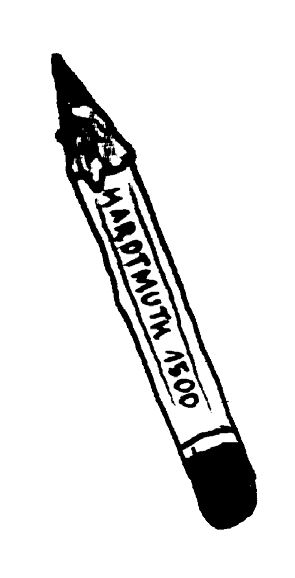
\includegraphics[height=0.3\textwidth]{images/chodz_pomaluj_moj_swiat.png}\vspace*{-0.305\textwidth}~~\\

  Trawy i drzewa są takie szare\\
  Barwę popiołu przybrały nieba\\
  W ciszy tak smutno szepcze zegarek\\
  O czasie, co mi go nie potrzeba\\

  \hspace*{4mm} Więc chodź, pomaluj mój świat\\
  \hspace*{4mm} Na żółto i na niebiesko\\
  \hspace*{4mm} Niech na niebie stanie tęcza\\
  \hspace*{4mm} Malowana twoją kredką\\
  \hspace*{4mm} Więc chodź, pomaluj mi życie\\
  \hspace*{4mm} Niech świat mój się zarumieni\\
  \hspace*{4mm} Niech mi zalśni w pełnym słońcu\\
  \hspace*{4mm} Kolorami całej Ziemi\\

  Za siódmą górą, za siódmą rzeką\\
  Moje sny zamieniasz na pejzaże\\
  Niebem się wlecze wyblakłe słońce\\
  Oświetla ludzkie, wyblakłe twarze\\

\end{minipage}
\begin{minipage}[t]{0.4\textwidth}
  a d \\
  G a \\
  C G \\
  d E a \\

  a d \\
  G a \\
  C G \\
  d E a \\

  C d\\
  F C\\
  C d\\
  F G\\
  C d\\
  F C\\
  C d\\
  F G\\

  a d \\
  G a \\
  C G \\
  d E a \\

\end{minipage}

\newpage
\section{Ciągle pada}\textcolor{lightgray}{\textit{Czerwone Gitary}}\\~\\
\begin{minipage}[t]{0.8\textwidth}
  Ciągle pada. Asfalt ulic jest dziś śliski jak brzuch ryby\\
  Mokre niebo się opuszcza coraz niżej\\
  Żeby przejrzeć się w zmarszczonej deszczem wodzie\\
  A ja? A ja chodzę, desperacko i na przekór wszystkim moknę\\
  Patrzę w niebo, chwytam w usta deszczu krople\\
  Patrzą na mnie rozpłaszczone twarze w oknie. To nic!\\
  \\
  \hspace*{3mm}Ciągle pada. Ludzie biegną, bo się bardzo boją deszczu\\
  \hspace*{3mm}Stają w bramie, ledwo się w tej bramie mieszcząc\\
  \hspace*{3mm}Ludzie skaczą przez kałuże na swej drodze\\
  \hspace*{3mm}A ja? A ja chodzę, nie przejmując się ulewą ani spiesząc\\
  \hspace*{3mm}Czując, jak mi krople deszczu usta pieszczą\\
  \hspace*{3mm}Ze złożonym parasolem idę pieszo. O tak!\\
  \\
  Ciągle pada. Alejkami już strumienie wody płyną\\
  Jakaś para się okryła peleryną\\
  Przyglądając się, jak mokną bzy w ogrodzie\\
  A ja? A ja chodzę w strugach wody, ale z czołem podniesionym\\
  Żadna siła mnie nie zmusza i nie goni\\
  Idę, niby zwiastun burzy, z kwiatem w dłoni. O tak!\\
  \\
  \hspace*{3mm}Ciągle pada. Nagle ogniem otworzyły się niebiosa\\
  \hspace*{3mm}Potem zaczął deszcz ulewny siec z ukosa\\
  \hspace*{3mm}Liście klonu się zatrzęsły w wielkiej trwodze\\
  \hspace*{3mm}A ja? A ja chodzę i nie straszna mi wichura ni ulewa\\
  \hspace*{3mm}Ani piorun, który trafił obok w drzewa\\
  \hspace*{3mm}Słucham wiatru, który wciąż inaczej śpiewa\\
\end{minipage}
\begin{minipage}[t]{0.2\textwidth}
  A fis\\
  fis D\\
  D E$^7$\\
  E$^7$ A fis\\
  fis D\\
  D E$^7$\\
  \\
  fis D\\
  D H\\
  H E\\
  fis D\\
  D H$^7$\\
  H$^7$ E\\

  A fis\\
  fis D\\
  D E$^7$\\
  E$^7$ A fis\\
  fis D\\
  D E$^7$\\
  \\
  fis D\\
  D H\\
  H E\\
  fis D\\
  D H$^7$\\
  H$^7$ E\\
\end{minipage}
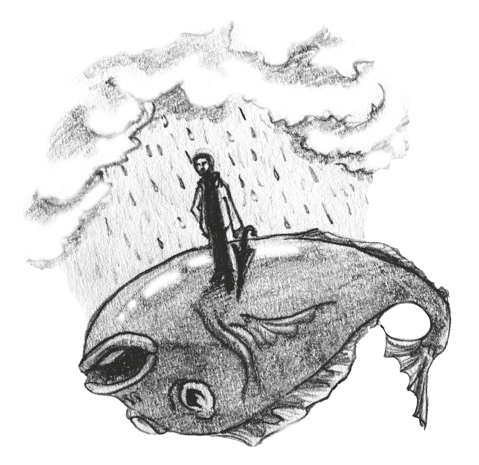
\includegraphics[height=0.4\textwidth,center]{images/ciagle_pada.png}\\

\newpage
\section{Country Roads}\textcolor{lightgray}{\textit{John Denver}}\\~\\
\begin{minipage}[t]{0.7\textwidth}
  Almost heaven, West Virginia\\
  Blue Ridge Mountains, Shenandoah River\\
  Life is old there, older than the trees\\
  Younger than the mountains, growin' like a breeze\\
  \\
  \hspace*{5mm}Country roads, take me home\\
  \hspace*{5mm}To the place I belong\\
  \hspace*{5mm}West Virginia, mountain mama\\
  \hspace*{5mm}Take me home, country roads\\
  \\
  All my memories gather 'round her\\
  Miner's lady, stranger to blue water\\
  Dark and dusty, painted on the sky\\
  Misty taste of moonshine, teardrop in my eye\\
  \\
  \hspace*{5mm}Country roads... \\
  \\
  I hear her voice in the mornin' hour, she calls me\\
  The radio reminds me of my home far away\\
  Drivin' down the road, I get a feelin'\\
  That I should've been home yesterday, yesterday\\
  \\
  \hspace*{5mm}Country roads... $\times$2\\
\end{minipage}
\begin{minipage}[t]{0.15\textwidth}
  G e\\
  D C G\\
  G e\\
  D C G\\

  G D\\
  e C\\
  G D\\
  C G\\

  G e\\
  D C G\\
  G e\\
  D C G\\

  ~\\

  e D G\\
  C G D\\
  e F C\\
  G D D$^7$\\

\end{minipage}
% \begin{minipage}[t]{0.15\textwidth}
% A fis\\
% E D A\\
% A fis\\
% E D A\\

% A E\\
% fis D\\
% A E\\
% D A\\

% A fis\\
% E D A\\
% A fis\\
% E D A\\

% ~\\

% fis E A\\
% D A E\\
% fis G D\\
% A E E$^7$\\
% \end{minipage}

\newpage
\section{Córka rybaka}\textcolor{lightgray}{\textit{Wały Jagiellońskie}}\\~\\
\begin{minipage}[t]{0.8\textwidth}
  Gdy księżyc świecił na niebie dla ciebie\\
  Poczułem miłość, co przyszła jak wiatr\\
  Me serce było w gorącej potrzebie\\
  Córką rybaka ty byłaś, ja - góral z Tatr\\
  Jelenie gdzieś nad jeziorem sennie ryczały\\
  Ryby w jeziorze już poszły dawno spać\\
  Rzekłaś wtedy do mnie: mój Mały\\
  Cóż ja ci mogę w tę parną, mazurską noc dać\\
  \\
  \hspace*{5mm}Córko rybaka, Mazura z Mazur\\
  \hspace*{5mm}Popatrz, jaki na jeziorze wody glazur\\
  \hspace*{5mm}Daj mi swe usta, weź mnie w ramiona\\
  \hspace*{5mm}Niech się przekonam, ile słodyczy jest w słowie\\
  \hspace*{5mm}Ilona\\
  \\
  Lato minęło, lecz uczucie ogniem płonie\\
  Choć dziś odległość tak wielka dzieli nas\\
  Wciąż jeszcze czuję na mym ciele twoje dwie dłon\\
  W uszach moich szumi woda, szemrze las\\
  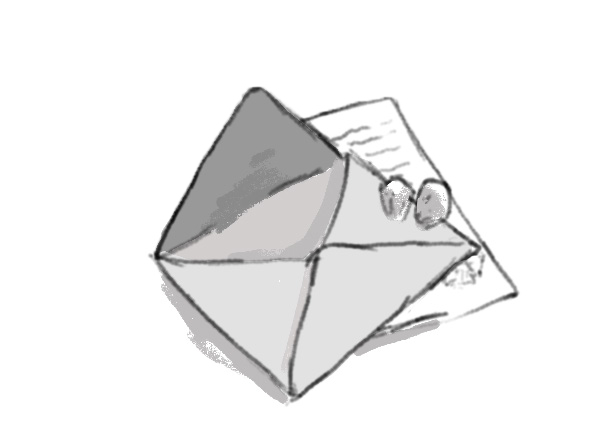
\includegraphics[height=2cm,right]{images/corka_rybaka.png}\vspace*{-21mm}\\
  Zakopane całe śniegiem zasypane\\
  A ty mi piszesz: na jeziorze gruba kra\\
  Przesyłasz całuski i dwie rybie łuski\\
  Zima przeminie, lato złączy serca dwa\\
\end{minipage}
\begin{minipage}[t]{0.2\textwidth}
  C G C\\
  C$^7$ G\\
  G F G$^7$\\
  G$^7$ G C\\
  C G C\\
  C$^7$ F\\
  F C a\\
  F G C\\
  \\
  C G\\
  G$^7$ C C$^7$\\
  F C a\\
  F G\\
  C\\

  C G C\\
  C$^7$ G\\
  G F G$^7$\\
  G$^7$ G C\\
  C G C\\
  C$^7$ F\\
  F C a\\
  F G C\\
\end{minipage}

\newpage
\section{Czarna stopa}\textcolor{lightgray}{\textit{Janusz Witkowski, Jakub Jugo; VII 2020}}\vspace*{1.5mm}\\
\begin{minipage}[t]{0.9\textwidth}
Był taki jeden co w Beskidy się pchał\\
Wszyscy myśleli że sandały tylko miał\\
Lecz nikomu wokół nie powiedział, że\\
Jeszcze ma w zanadrzu stopy dwie \vspace*{1.5mm}
\\
W Beskidzie Niskim mnóstwo błota jest\\
Nasz bohater zrobił w błocie butów chrzest\\
Cały dzień by błocił swe sandały, lecz\\
W końcu je przegonił "z nóg mi precz!" \vspace*{1.5mm}
\\
\hspace*{5mm}(Czarna Stopa $\times$16)\\
\hspace*{5mm}Będą śmiać się, będą szydzić, będą mówić Czarna Stopa\\
\hspace*{5mm}Gołe pięty, nagie palce, a na stopach kawał chłopa \vspace*{1.5mm}
\\
Dziwny to koleś, co tu więcej gadać\\
Ściąga ubrania gdy zaczyna padać\\
Kiedy brud narasta (Czarna Stopa $\times$2)\\
W strumyku myje się mydłem z błota \vspace*{1.5mm}
\\
\hspace*{5mm}(Czarna Stopa $\times$16)\\
\hspace*{5mm}Będą śmiać się, będą szydzić, będą mówić Czarna Stopa\\
\hspace*{5mm}Będą mieszać z błotem pomysł, bosa stopa - wielka wtopa \vspace*{1.5mm}
\\
Niestraszne mu zaostrzone kamienie\\
Super-Żuki, czy Pająki Skurwiele\\
Wyciek gazu go nie ruszy, kolego\\
Więc nie masz na co liczyć, barszczu sosnowskiego.\\
(Barszczu, barszczu sosnowskiego $\times$4) \vspace*{1.5mm}
\\
Może nie znał z sanitarnych wiadomości\\
Przykrych przypadłości (barszczu, barszczu sosnowskiego)\\
Każdego dnia narażać się na krach\\
By z okna samochodu patrzeć w dal \vspace*{1.5mm}
\\
\hspace*{5mm}(Czarna Stopa $\times$16)\\
\hspace*{5mm}Będą śmiać się, będą szydzić, będą mówić Czarna Stopa\\
\hspace*{5mm}Rzucą gościa w szosę, żeby Czarna Stopa złapał stopa \vspace*{1.5mm}
\\
Lecz gdy przychodzi do schroniska wbić\\
Buty turystom poczynają gnić\\
Można chyba rzec że są głupi fest\\
Czarna Stopa to więc jakiś mesjasz jest \vspace*{1.5mm}
\\
\hspace*{5mm}(Czarna Stopa $\times$32)\\
\hspace*{5mm}Będzie śmiał się, będzie szydził, będzie górą Czarna Stopa\\
\hspace*{5mm}Tych buciarzy czeka mycie bo nie wiedzą co to życie\\
\hspace*{5mm}Kiedy pierwsza śnieżka spadnie barany do miast powrócą\\
\hspace*{5mm}A Czarna Stopa machnie ręką i ucieknie przed północą \\
\hspace*{5mm}(Czarna Stopa $\times$5)\\
\end{minipage}
\begin{minipage}[t]{0.1\textwidth}
\end{minipage}

\newpage
\section{Czarny blues o czwartej nad ranem}\textcolor{lightgray}{\textit{SDM}}\\~\\
\begin{minipage}[t]{0.7\textwidth}

  \hspace*{4mm} Czwarta nad ranem, może sen przyjdzie\\
  \hspace*{4mm} Może mnie odwiedzisz\\
  \hspace*{4mm} Czwarta nad ranem, może sen przyjdzie\\
  \hspace*{4mm} Może mnie odwiedzisz\\

  Czemu cię nie ma na odległość ręki\\
  Czemu mówimy do siebie listami\\
  Gdy ci to śpiewam - u mnie pełnia lata\\
  Gdy to usłyszysz - będzie środek zimy\\

  Czemu się budzę o czwartej nad ranem\\
  I włosy twoje próbuję ugłaskać\\
  Lecz nigdzie nie ma twoich włosów\\
  Jest tylko blada nocna lampka\\
  Łysa śpiewaczka\\

  Śpiewamy bluesa, bo czwarta nad ranem\\
  Tak cicho, by nie zbudzić sąsiadów\\
  Czajnik z gwizdkiem świruje na gazie\\
  Myślałby kto, że rodem z Manhattanu\\

  \hspace*{4mm} Czwarta nad ranem ... \\

  Herbata czarna myśli rozjaśnia\\
  A list twój sam się czyta\\
  Że można go śpiewać - za oknem mruczą bluesa\\
  Topole z Krupniczej\\

  I jeszcze strażak wszedł na solo\\
  Ten z Mariackiej Wieży\\
  Jego trąbka jak księżyc biegnie nad topolą\\
  Nigdzie się jej nie spieszy\\

  \hspace*{4mm} Już piąta, może sen przyjdzie\\
  \hspace*{4mm} Może mnie odwiedzisz\\
  \hspace*{4mm} Już piąta, może sen przyjdzie\\
  \hspace*{4mm} Może mnie odwiedzisz\\

\end{minipage}
\begin{minipage}[t]{0.3\textwidth}
  A cis\\
  D A\\
  E fis\\
  D E A\\

  A E\\
  fis cis\\
  D A\\
  D E\\

  A E\\
  fis cis\\
  D A\\
  D E\\
  fis\\

  A E\\
  fis cis\\
  D A\\
  D E\\

  ~\\

  A E\\
  fis cis\\
  D A\\
  D E\\

  A E\\
  fis cis\\
  D A\\
  D E\\

  A cis \\
  D A \\
  E fis\\
  D E A\\
\end{minipage}

\newpage
\section{Czas mierzę niebem}\textcolor{lightgray}{\textit{Julia Błaszczyk (Julka Retro), Włodzimierz Mizia\\}}~\\
\begin{minipage}[t]{0.6\textwidth}
  Czas mierzę niebiem			\\
  Nad głową toczy błękit swój			\\
  Pytam obłoków o ciebie			\\
  Prastary nieboskłonu zwój		\\
  Inne obłoki nad tobą			\\
  Odpowiedź tak brzmi			\\
  Już inne chmury nad twoją głową			\\

  Głaszczę spód nieba\\
  Niebo grzbietem dotyka gwiazd\\
  Pytam nocy Czego Ci trzeba\\
  W studni nade mną szukam rad\\
  Te same gwiazdy nad nami\\
  Odpowiedź jej brzmi\\
  Te same gwiazdy nam nad głowami\\

  Jeśli z tych samych gwiazd		\\
  Błyszczy nam w oczach jeden blask\\
  I nocą pogłowie chodzą nam		\\
  Te same refleksy dalekich lat		\\
  Przyznaj, że możemy dalej razem iść\\
  Ramię w ramię i myśl w myśl				\\

  Podnoszę głowę				\\
  Błękit schyla do mnie swój pysk		\\
  Widzisz jego drugą połowę			\\
  Ten sam stary złoty dysk			\\
  To samo słońce zalewa nas		\\
  Inaczej nie może być			\\
  Jedno słońce daje nam czas				\\
\end{minipage}
\begin{minipage}[t]{0.4\textwidth}
  C\\
  F	\\
  C\\
  F\\
  D\\
  F\\
  C F\\

  C\\
  F	\\
  C\\
  F\\
  D\\
  F\\
  C F\\

  a\\
  F\\
  a\\
  F\\
  D\\
  F C\\

  C\\
  F	\\
  C	\\
  F\\
  D\\
  F\\
  C F C\\
\end{minipage}

\newpage
\section{Czerwony jak cegła}\textcolor{lightgray}{\textit{Dżem}}\\~\\
\begin{minipage}[t]{0.8\textwidth}
  Nie wiem jak mam to zrobić, ona zawstydza mnie\\
  Strach ma tak wielkie oczy, wokół ciemno jest\\
  Czuje się jak Beniamin i udaję, że śpię\\
  Może walnę kilka drinków, może nakręcą mnie\\
  Nakręcą mnie\\
  \\
  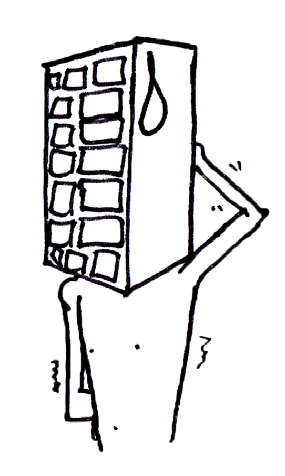
\includegraphics[height=5cm,right]{images/czerwony_jak_cegla.png}\vspace*{-51mm}\\
  Nie wiem jak mam to zrobić, by mężczyzną się stać\\
  I nie wypaść ze swej roli tego, co pierwszy raz\\
  Gładzę czule jej ciało, skradam się do jej ust\\
  Wiem, że to jeszcze za mało, aby ciebie mieć\\
  Aby mieć\\
  \\
  \hspace*{5mm}Czerwony jak cegła, rozgrzany jak piec\\
  \hspace*{5mm}Muszę mieć, muszę ją mieć\\
  \hspace*{5mm}Nie mogę tak odejść, gdy kusi mnie grzech\\
  \hspace*{5mm}Muszę mieć, muszę ją mieć\\
  \\
  Nie wiem jak to się stało, ona chyba już śpi\\
  Leżę obok pełen wstydu, krótki to był zryw\\
  Będzie lepiej, gdy pójdę, nie chcę patrzeć jej w twarz\\
  Może kiedyś da mi szansę spróbować jeszcze raz\\
  Jeszcze jeden, jeden raz\\
\end{minipage}
\begin{minipage}[t]{0.2\textwidth}
  E A E H$^7$\\
  E A E H\\
  E A E H$^7$\\
  E A H E\\
  (A) E H$^7$\\

  E A E H$^7$\\
  E A E H\\
  E A E H$^7$\\
  E A H E\\
  (A) E\\

  A\\
  E (A) E\\
  H (C) cis A\\
  E (A) E H$^7$\\
  \\
  E A E H$^7$\\
  E A E H\\
  E A E H$^7$\\
  E A H E\\
  (A) E\\

\end{minipage}

\newpage
\section{Człowiek jam niewdzięczny}\textcolor{lightgray}{\textit{Czesław Niemen}}\\~\\
\begin{minipage}[t]{0.6\textwidth}
  ~\\
  Dzień za dniem, jak wartki potok czas\\
  Zacieśnia krąg istnienia mego\\
  Dzień za dniem, uciekam dalej, dalej, dalej\\
  Mych złudnych pragnień splot upada\\
  \\
  \hspace*{5mm}A wokoło Wszechświat\\
  \hspace*{5mm}Bezgraniczny, niepojęty\\
  \hspace*{5mm}Nieskończony ogród żyzny\\
  \hspace*{5mm}Myśli wiecznej Arcydzieło\\
  \hspace*{5mm}Uszanować chciałbym Niebo\\
  \hspace*{5mm}Ziemi czoła skłonić\\
  \hspace*{5mm}Ale człowiek jam niewdzięczny\\
  \hspace*{5mm}Że niedoskonały\\
  \\
  ~\\
  Nonsensami karmią się nawzajem\\
  Spraw komicznych omotani, omotani siecią\\
  Wstyd mi za tych, co nie mając wstydu\\
  Zapomnieli, że u kresu groby nas zrównają\\
\end{minipage}
\begin{minipage}[t]{0.4\textwidth}
  (a (G) a)\\
  a G\\F (a(G)a)\\
  a G\\F a\\

  (G) C d\\F C\\C d\\F C\\
  C d\\F C\\C d\\F C\\

  (a (G) a)\\
  a G\\F (a(G)a)\\
  a G\\F a\\
\end{minipage}
\\
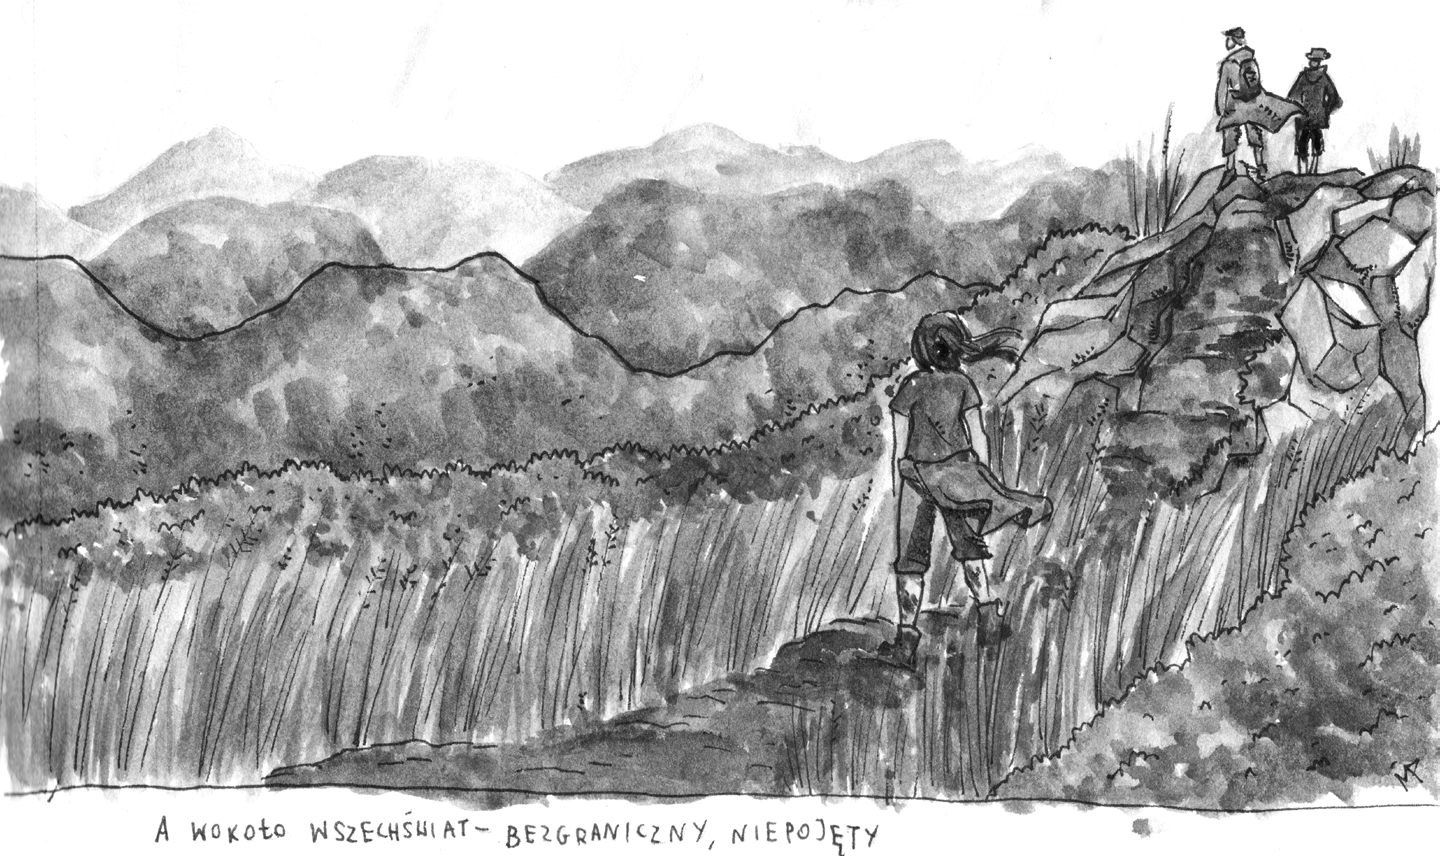
\includegraphics[width=\textwidth,center]{images/czlowiek_jam_niewdzieczny.png}\\

\newpage
\section{Człowiek z liściem}\textcolor{lightgray}{\textit{Elektryczne Gitary}}\\~\\
\begin{minipage}[t]{0.5\textwidth}
  Wsiadł do autobusu\\
  Człowiek z liściem na głowie\\
  Nikt go nie poratuje\\
  Nikt mu nic nie powie\\
  Tylko się każdy gapi\\
  Tylko się każdy gapi i nic\\
  \\
  Siedzi w autobusie\\
  Człowiek z liściem na głowie\\
  O liściu w swych rzadkich włosach\\
  Nieprędko się dowie\\
  Tylko się w okno gapi\\
  Tylko się w okno gapi i nic\\
  \\
  \hspace*{5mm}Uważaj, to nie chmury\\
  \hspace*{5mm}To Pałac Kultury\\
  \hspace*{5mm}Liście lecą z drzew\\
  \hspace*{5mm}Liście lecą z drzew\\
  \\
  I tak siedzi w autobusie\\
  Człowiek z liściem na głowie\\
  Nikt go nie poratuje\\
  Nikt mu nic nie powie\\
  Tylko się każdy gapi\\
  Tylko się każdy gapi i nic\\
  \\
  Wsiadł drugi podobny\\
  Nad człowiekiem się zlitował\\
  Tamten się pogłaskał w główkę\\
  Liścia sobie schował\\
  Bo ja, mówi, jestem z lasu\\
  Bo ja, mówi, jestem z lasu i już\\
  \\
  \hspace*{5mm}Uważaj, to nie chmury. . .\\
\end{minipage}
\begin{minipage}[t]{0.5\textwidth}
  a\\
  e\\
  G\\
  D\\
  F G\\
  C F C E\\
  \\
  a\\
  e\\
  G\\
  D\\
  F G\\
  C F C E\\
  \\
  d G\\
  C F C\\
  G\\
  F C F C E\\
  \\
  a\\
  e\\
  G\\
  D\\
  F G\\
  C F C E\\
  \\
  a\\
  e\\
  G\\
  D\\
  F G\\
  C F C E\\
\end{minipage}

\newpage
\section{Cztery piwka}\textcolor{lightgray}{\textit{Jerzy Porębski}}\\~\\
\begin{minipage}[t]{0.85\textwidth}
  Ze Świnoujścia do Walvis Bay droga nie była krótka\\
  A po dwóch dobach, albo mniej, już się skończyła wódka\\
  Do brydża!, krzyknął Siwy Flak i z miejsca rzekł Dwa piki\\
  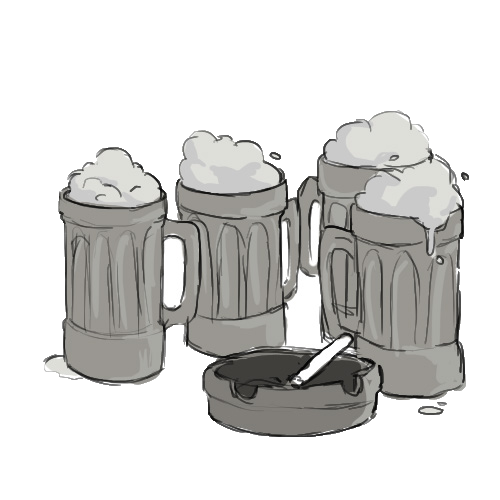
\includegraphics[height=35mm,right]{images/cztery_piwka.png}\vspace*{-36mm}\\
  A ochmistrz w telewizor wlał nie byle jakie siki\\
  \\
  \hspace*{5mm}Cztery piwka na stół, w popielniczkę pet\\
  \hspace*{5mm}Jakąś Damę roześmianą Król przytuli wnet\\
  \hspace*{5mm}Gdzieś między palcami sennie płynie czas\\
  \hspace*{5mm}Czwarta ręka, Króla bije As\\
  \\
  A w karcie tylko jeden As i nic poza tym nie ma\\
  Ale nie powiem przecież Pas, może zagrają szlema\\
  Kontra mu rzekłem, taki bluff, by nieco spuścił z tonu\\
  A Fred mu na to Cztery trefl!, przywalił bez pardonu\\
  \\
  A mój w dwa palce obtarł nos, to znaczy: nie ma nic\\
  I wtedy Flak, podnosząc głos, powiedział Cztery pik!\\
  I kiedy jeszcze cztery Króle pokazał mu jak trza\\
  To Fred z renonsem Siedem pik, powiedział Niech gra Flak!\\
  \\
  A ja mu Kontra, on mi Re, ja czuję pełen luz,\\
  Bo widzę w moich kartach, że jest atutowy tuz\\
  Więc strzelam! Kiedy karty Fred wyłożył mu na blat\\
  To każdy mógł zobaczyć, jak Siwego Flaka trafia szlag\\
  \\
  Już nie pamiętam, ile dni w miesiące złożył czas\\
  Morszczuki dosyć dobrze szły i grało się nie raz\\
  Lecz nigdy więcej Siwy Flak, klnę na jumprowe wszy\\
  Choćbyś go prosił tak, czy siak, nie zasiadł już do gry\\
  \\
  \hspace*{5mm}W popielniczkę pet, cztery piwka na stół\\
  \hspace*{5mm}Już tej Damy roześmianej nie przytuli Król\\
  \hspace*{5mm}Gdzieś nam się zapodział atutowy As\\
  \hspace*{5mm}Tego Szlema z nami wygrał czas\\
\end{minipage}
\begin{minipage}[t]{0.15\textwidth}
  e\\e\\e\\H$^7$\\

  E A\\
  H$^7$ E\\
  E$^7$ A\\
  H$^7$ e\\

  e\\e\\e\\H$^7$\\

  e\\e\\e\\H$^7$\\

  e\\e\\e\\H$^7$\\

  e\\e\\e\\H$^7$\\

  E A\\
  H$^7$ E\\
  E$^7$ A\\
  H$^7$ e\\

\end{minipage}

\newpage
\section{Czy ci ludzie mogą wsiadać?}\textcolor{lightgray}{\textit{Trójkowy Klub Artystycznych Dusz, XI 2018}}\\~\\
\begin{minipage}[t]{0.8\textwidth}
  A gdy już wsiądą, raz i drugi \\
  Kobiety po trasie, mężczyźni po przejściach \\
  Kąt wynajdują gdzieś w pociągu \\
  I łapią, i łapią trochę szczęścia \vspace*{1.5mm}\\
  \hspace*{4mm}Ludzie wsiadają, jest ich coraz więcej \\
  \hspace*{4mm}Już drzwi się nie domykają, konduktor wysiadł z pociągu \\
  \hspace*{4mm}Opadły mu nogi i ręce\\
  \hspace*{4mm}A gdy straci cierpliwość w uniformie ta postać \\
  \hspace*{4mm}Lepiej uciec, bo w ryj możesz dostać \\

  \hspace*{7mm}Czy ci ludzie mogą wsiadać? Chyba nie \\
  \hspace*{7mm}Czy się drzwi mogą wyłamać? Itp. \\
  \hspace*{7mm}Chyba dzisiaj wracasz sama... To był błąd \\
  \hspace*{7mm}Czy ci ludzie mogą wsiadać? Ależ skąd! \\

  A gdy się czasem usiąść uda\\
  Kobietom po przejściach, mężczyznom po trasie\\
  Żarcie wyjmują, począwszy od wafli\\
  A kończąc na suchej kiełbasie\vspace*{1.5mm}\\
  \hspace*{4mm}A na dodatek w ruch idzie gitara\\
  \hspace*{4mm}Piosenki niewyszukane, masa fałszywych dźwięków\\
  \hspace*{4mm}Och za co, och za co ta kara?!\\
  \hspace*{4mm}A gdy przyjdzie wybierać na peronie czy zostać\\
  \hspace*{4mm}Lepiej uciec, by z łokcia nie dostać\\

  \hspace*{7mm}Czy ci ludzie mogą wsiadać? Chyba nie\\
  \hspace*{7mm}Czy się drzwi mogą wyłamać? Itp.\\
  \hspace*{7mm}Chciałaś dzisiaj wracać sama... To był błąd\\
  \hspace*{7mm}Czy ci ludzie mogą wsiadać? Ależ skąd!\\
\end{minipage}
\begin{minipage}[t]{0.2\textwidth}
  d a\\
  E a\\
  d a\\
  E a (E a)\vspace*{1.5mm}\\
  d a\\
  d a d a\\
  E a (E a)\\
  d a\\
  E a (E a)\\

  d\\
  a\\
  E\\
  a (E a)\\

  d a\\
  E a\\
  d a\\
  E a (E a)\vspace*{1.5mm}\\
  d a\\
  d a d a\\
  E a (E a)\\
  d a\\
  E a (E a)\\
  \\
  d\\
  a\\
  E\\
  a (E a)\\
\end{minipage}
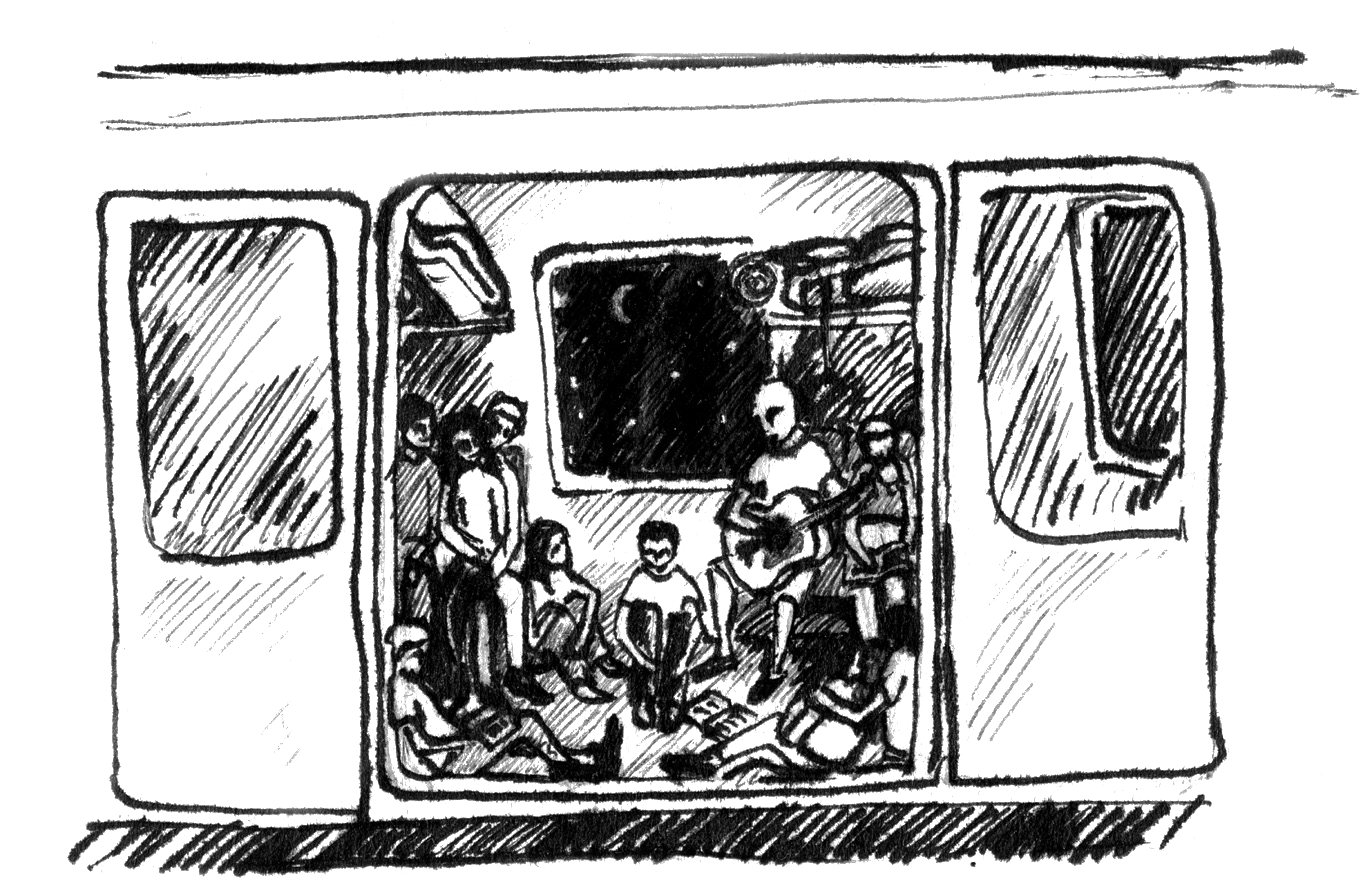
\includegraphics[height=5.2cm, center]{images/czy_ci_ludzie.png}

\newpage
\section{Czy te oczy mogą kłamać}\textcolor{lightgray}{\textit{Raz Dwa Trzy}}\\~\\
\begin{minipage}[t]{0.85\textwidth}
  A gdy się zejdą, raz i drugi\\
  Kobieta po przejściach, mężczyzna z przeszłością\\
  Bardzo się męczą, męczą przez czas długi\\
  Co zrobić, co zrobić z tą miłością\\

  \hspace*{1mm} On już je zna, już zna te dziewczyny\\
  \hspace*{1mm} Z poszarpanymi nerwami, co wracają nad ranem nie same\\
  \hspace*{1mm} On już słyszał o życiu złamanym\\

  \hspace*{1mm} Ona już wie, już zna tę historię\\
  \hspace*{1mm} Że żona go nie rozumie, że wcale ze sobą nie śpią\\
  \hspace*{1mm} Ona na pamięć to umie\\

  \hspace*{4mm} A gdy przyjdzie zapomnieć i w pamięci to zatrzeć\\
  \hspace*{4mm} Lepiej milczeć przytomnie i patrzeć\\
  \hspace*{6mm} Czy te oczy mogą kłamać? Chyba nie\\
  \hspace*{6mm} Czy ja mógłbym serce złamać? Itp.\\
  \hspace*{6mm} Kiedyś to zrozumiesz sama… To był błąd\\
  \hspace*{6mm} Czy te oczy mogą kłamać? Ależ skąd\\

  A gdy się czasem w życiu uda\\
  Kobiecie z przeszłością, mężczyźnie po przejściach\\
  Kąt wynajdują gdzieś u ludzi\\
  I łapią, i łapią trochę szczęścia\\

  \hspace*{1mm} On zapomina na rok te dziewczyny\\
  \hspace*{1mm} Z bardzo długimi nogami, co wracają nad ranem nie same\\
  \hspace*{1mm} Woli ciszę z radzieckim szampanem\\

  \hspace*{1mm} Ona już ma, już ma taką pewność\\
  \hspace*{1mm} O którą wszystkim wam chodzi, zasypia bez żadnych proszków\\
  \hspace*{1mm} Wino w lodówce się chłodzi\\

\end{minipage}
\begin{minipage}[t]{0.15\textwidth}
  d a\\
  E a\\
  d a\\
  E a (E a)\\

  d a\\
  d a d a\\
  E a (E a)\\

  d a\\
  d a\\
  E a (E a)\\

  d a\\
  E a (E a)\\
  d\\
  a\\
  E\\
  a (E a) \\

  d a\\
  E a\\
  d a\\
  E a (E a)\\

  d a\\
  d a d a\\
  E a (E a)\\

  d a\\
  d a\\
  E a (E a)\\

\end{minipage}

\newpage
\section{Debilna piosenka}\textcolor{lightgray}{\textit{Zioma}}\\~\\
\begin{minipage}[t]{0.85\textwidth}
  Debilna piosenka, sama się śpiewa, sama się pamięta\\
  Piosenka debila, którego cieszy w życiu każda chwila\\
  Gdy może z góry pod górę, z góry pod górę…\\
  \\
  Nucę ją w głowie, kiedy pod górę, gdy pod nią wchodzę sobie\\
  Szaleńczo ją śpiewam, gdy zaraz potem z tej góry zbiegam\\
  Potem z powrotem z potem, potem z powrotem z potem, tarararam\\
  \\
  Debilna piosenka, sama się śpiewa, sama się pamięta\\
  Piosenka wariata, który pionowo w kółko lata\\
  Bo jak inaczej nazwać idiotę, co pod górę wchodzi, by zaraz zejść z\\
  powrotem?\\
  To maniak jest bez wahania, opętała go mania wspinania\\
  Mania wspinania mania mania... mania czegoś do wspinania, tarararam\\
  \\
  I wszystko by było cacy, gdyby nie ten jego plecaczek\\
  A jest to około dwieście kilo, z którym na plecach miota się debilo\\
  (I tu debilo na wykrotach się miota\\
  I gdy pot mu oczy zalewa on i tak ją sobie śpiewa\\
  Ją czyli czą? No oczywiście…)\\
  \\
  Debilną piosenkę, która mu szlak wytycza przez tą mękę\\
  Nuci ją sobie tamtamtararamta, piosenkę nieszkodliwego palanta\\
  \\
  (A teraz wątek osobisty)\\
  I gdyby nawet mnie zamknęli w gąbką wykładanej celi\\
  Mało mnie to obchodzi, byle by tam było na co wchodzić\\
  A potem schodzić, a potem wchodzić, schodzić, wchodzić, schodzić\\
  \\
  Debilna piosenka, sama się śpiewa, sama się pamięta\\
  Piosenka szajbusa, co wchodzi na wszystko, co się nie rusza\\
  (A jak się rusza to i tak wchodzi, co mu szkodzi\\
  Pojedzie do Łodzi, najwyżej coś spłodzi)\\

  I kiedyś wielkim spychaczem, spychnę wszystkie góry świata w jeden placek\\
  Potem podrapię się w głowę i z tych gór wszystkich jedną wielką zrobię\\
  Każdy nieprzystosowany wejdzie na nią tylko raz\\
  I będziecie mieli z nami spokój już na cały czas, na cały czas, czasczas..\\
  \\

\end{minipage}
\begin{minipage}[t]{0.15\textwidth}
  C$^9$$\star$C$^9$G\\
  ~\\
  ~\\

  \chord{t}{n,n,p3,p2,p3,p3}{$\star$}
\end{minipage}
\newpage
\begin{minipage}[t]{0.9\textwidth}
  Debilom potakiwać trzeba, macie rację, niech sobie pośpiewam\\
  Pomyślcie lecz przez chwilę, kto z was jest jeszcze takim jak ja\\
  Na dół na dół, do góry do góry…\\
  \\
  Debilna piosenka, sama się śpiewa sama się pamięta\\
  Piosenka debila, którego cieszy w życiu każda chwila\\
  Debilna piosenka, sama się śpiewa, sama się pamięta\\
  Piosenka debila, któremu z pyska cieknie ślina\\
  Gdy może z góry pod górę, z góry pod górę…\\
  \\
  Debilna piosenka, sama się śpiewa, sama się pamięta\\
  Nienienienie opamięta\\
\end{minipage}
\begin{minipage}[t]{0.1\textwidth}
  C$^9$$\star$C$^9$G\\
\end{minipage}

% \newpage
\section{Dni, których jeszcze nie znamy}\textcolor{lightgray}{\textit{Marek Grechuta}}\\~\\
\begin{minipage}[t]{0.7\textwidth}
  Tyle było dni do utraty sił\\
  Do utraty tchu tyle było chwil\\
  Gdy żałujesz tych, z których nie masz nic\\
  Jedno warto znać, jedno tylko wiedz, że\\
  \\
  \hspace*{10mm}Ważne są tylko te dni\\
  \hspace*{10mm}Których jeszcze nie znamy\\
  \hspace*{10mm}Ważnych jest kilka tych chwil\\
  \hspace*{10mm}Tych na które czekamy\\
  \\
  Pewien znany ktoś, kto miał dom i sad\\
  Zgubił nagle sens i w złe kręgi wpadł\\
  Choć majątek prysł, on nie stoczył się\\
  Wytłumaczyć umiał sobie wtedy właśnie, że\\
  \\
  % \hspace*{5mm}Ważne są tylko. . . $\times $2\\
  % \\
  \hspace*{5mm}Jak rozpoznać ludzi, których już nie znamy?\\
  \hspace*{5mm}Jak pozbierać myśli z tych nieposkładanych?\\
  \hspace*{5mm}Jak oddzielić nagle serce od rozumu?\\
  \hspace*{5mm}Jak usłyszeć siebie pośród śpiewu tłumu?\vspace*{2mm}
  \\
  \hspace*{5mm}Jak rozpoznać ludzi, których już nie znamy?\\
  \hspace*{5mm}Jak pozbierać myśli z tych nieposkładanych?\\
  \hspace*{5mm}Jak odnaleźć nagle radość i nadzieję?\\
  \hspace*{5mm}Odpowiedzi szukaj, czasu jest tak wiele\\

  % \hspace*{5mm}Ważne są tylko. . . $\times $2\\
\end{minipage}
\begin{minipage}[t]{0.3\textwidth}
  a C G C\\
  d A C G\\
  a C G C\\
  d A C G\\

  F d G \\
  a F G C\\
  F d G \\
  a F G C\\

  a C G C\\
  d A C G\\
  a C G C\\
  d A C G\\

  % ~\\

  a e C G\\
  a e C G\\
  d a F C\\
  a e C G\vspace*{2mm}

  a e C G\\
  a e C G\\
  d a F C\\
  a e C G\\
\end{minipage}

\newpage
\section{Do kołyski}\textcolor{lightgray}{\textit{Dżem}}\\~\\
\begin{minipage}[t]{0.7\textwidth}
  Żyj z całych sił i uśmiechaj się do ludzi\\
  Bo nie jesteś sam\\
  Śpij, nocą śnij, niech zły sen Cię nigdy więcej nie obudzi\\
  Teraz śpij\\

  Niech dobry Bóg zawsze Cię za rękę trzyma\\
  Kiedy ciemny wiatr\\
  Porywa spokój, siejąc smutek i zwątpienie\\
  Pamiętaj, że...\\

  \hspace*{5mm}Jak na deszczu łza\\
  \hspace*{5mm}Cały ten świat nie znaczy nic\\
  \hspace*{5mm}A nic\\
  \hspace*{5mm}Chwila która trwa\\
  \hspace*{5mm}Może być najlepszą z Twoich chwil\\
  \hspace*{5mm}Najlepszą z Twoich chwil\\

  Idź własną drogą, bo w tym cały sens istnienia\\
  Żeby umieć żyć\\
  Bez znieczulenia, bez niepotrzebnych niespełnienia\\
  Myśli złych\\

  \hspace*{5mm}Jak na deszczu łza... $\times$2\\

\end{minipage}
\begin{minipage}[t]{0.3\textwidth}
  h\\
  (eA) h\\
  h\\
  (eA) h\\

  h\\
  (eA) h\\
  h\\
  (eA) D\\

  e A\\
  h e \\
  A (G)\\
  e A\\
  h e\\
  A\\

  h\\
  (eA) h\\
  h\\
  (eA) D\\
\end{minipage}

\newpage
\section{Do serca przytul psa}\textcolor{lightgray}{\textit{Jan Kaczmarek~~~~~~~~~~~~~~~~~~~~~~}} \vspace*{-0.06\textheight}\\
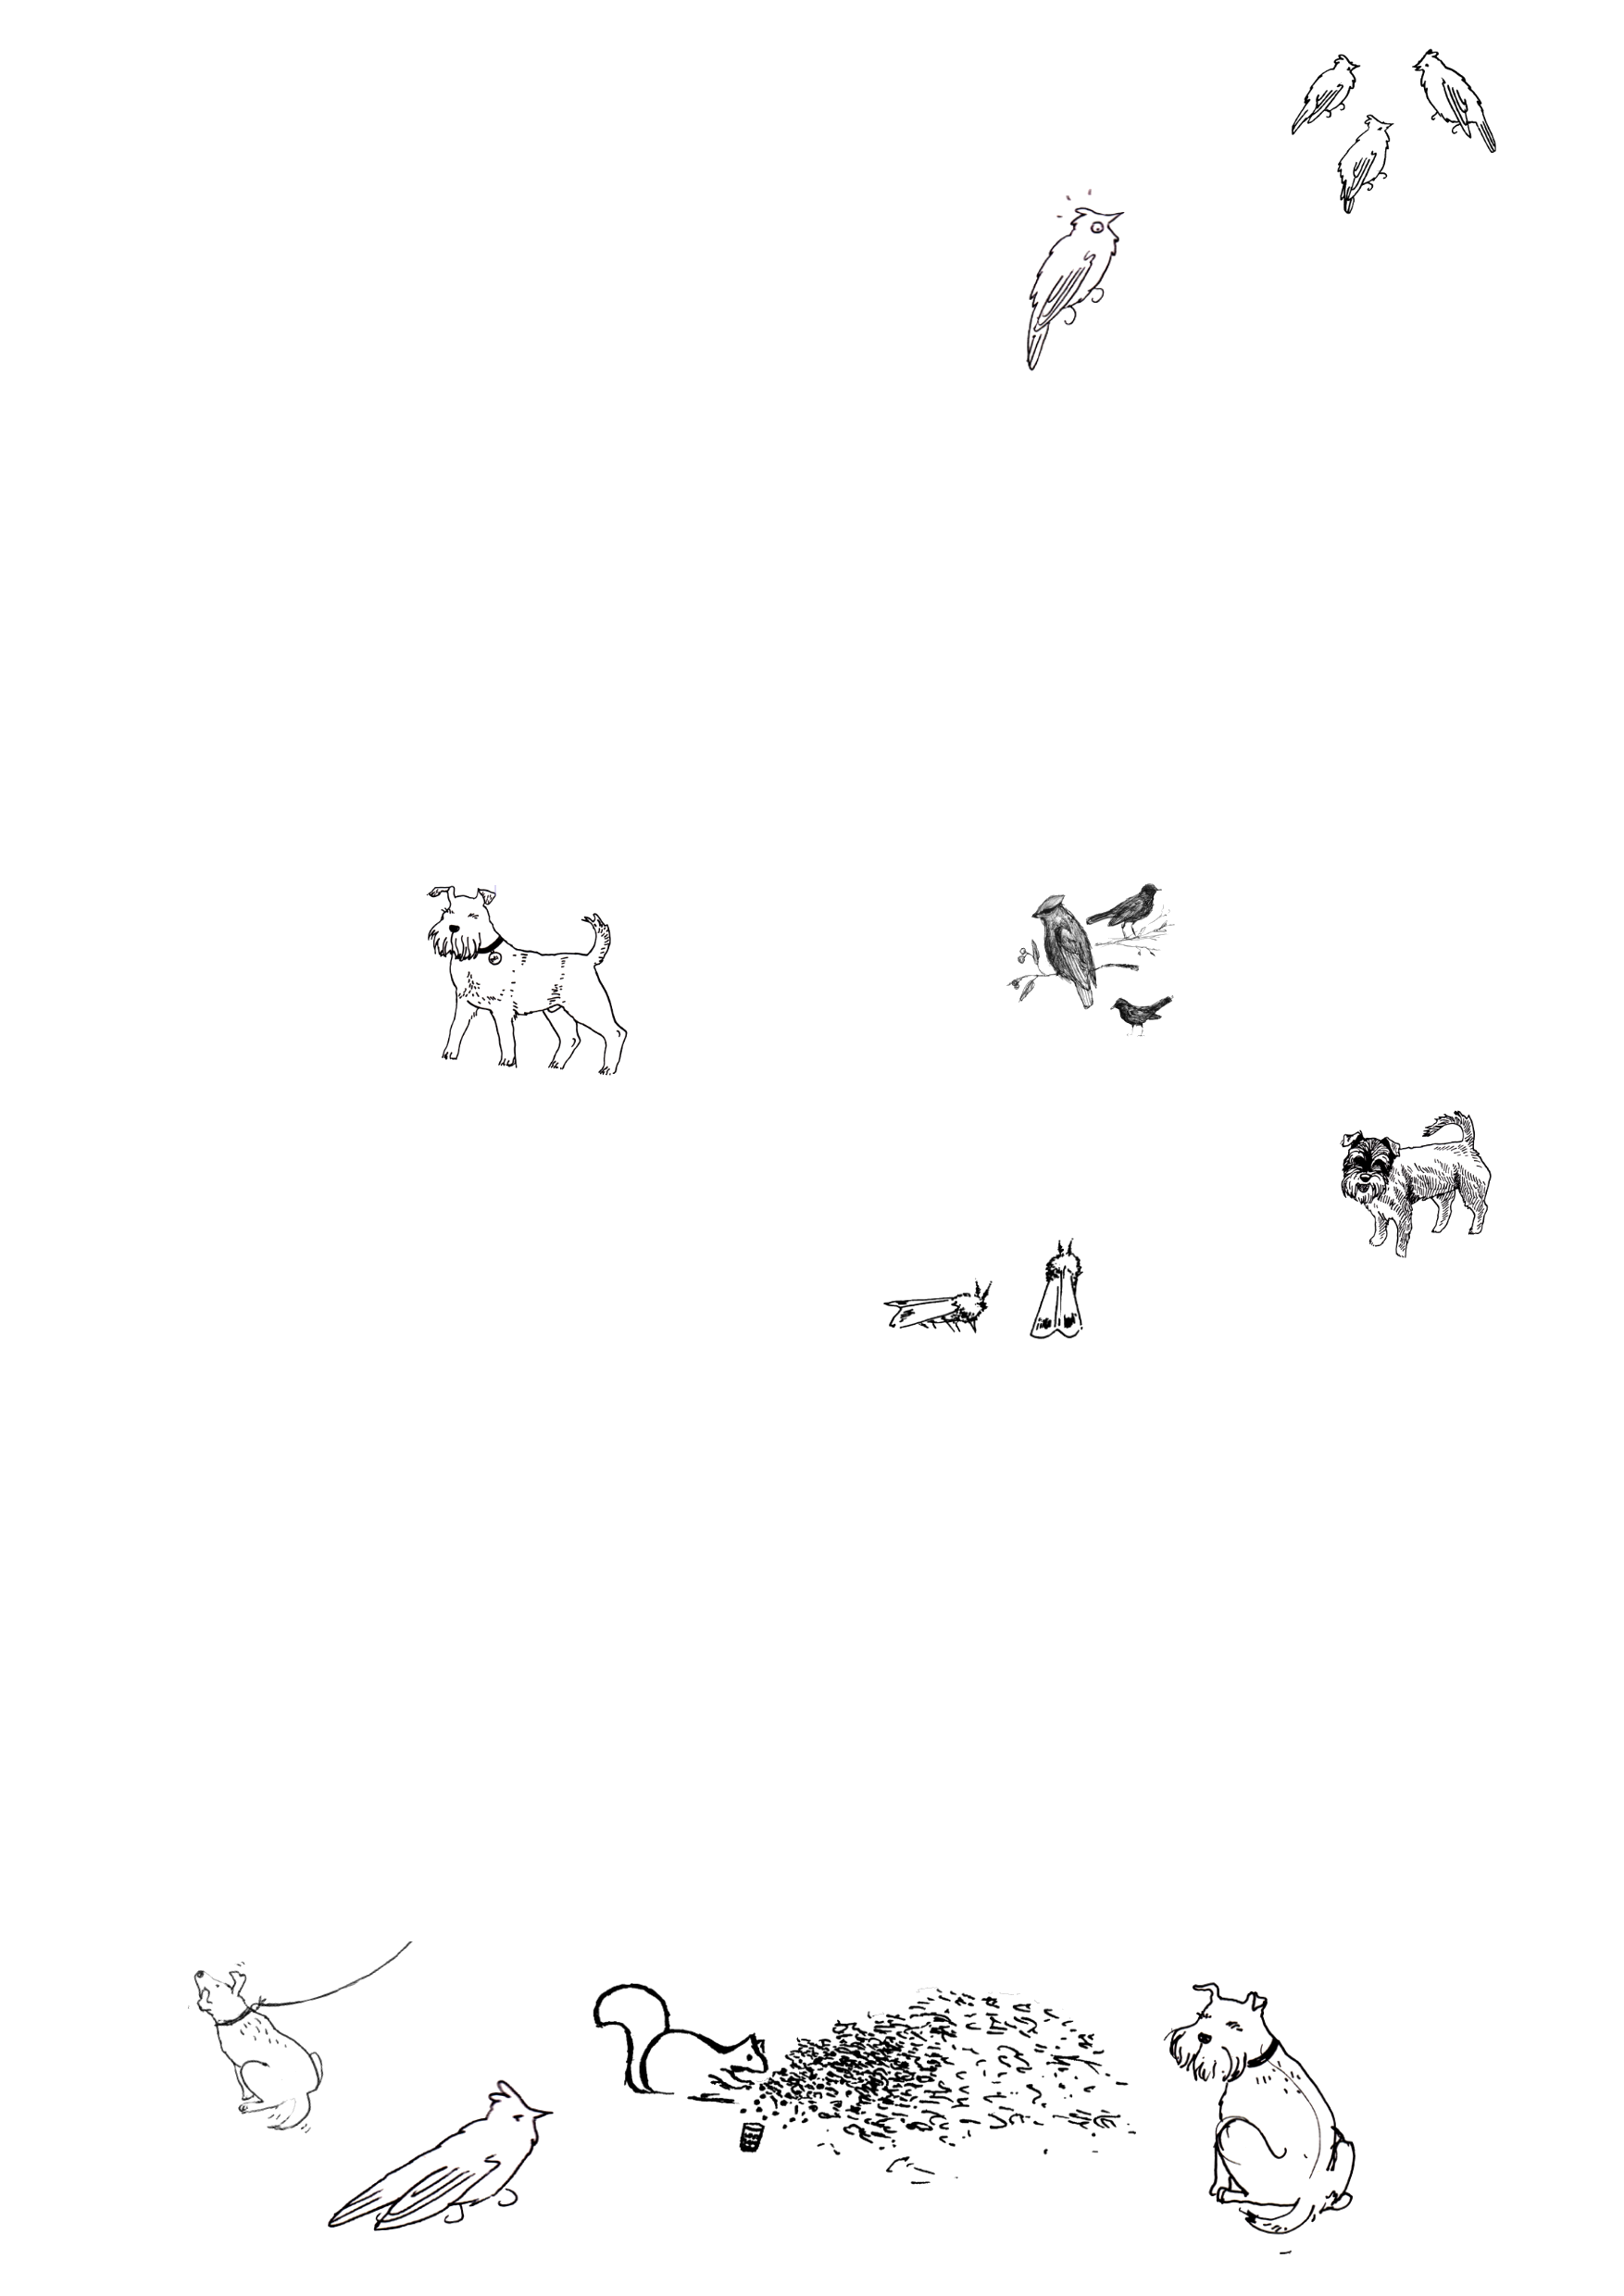
\includegraphics[height=1.05\textheight]{images/do_serca_przytul_psa_gimp.png}\vspace*{-0.98\textheight}\\
\begin{minipage}[t]{0.8\textwidth}
  Zanim zdechnie w oceanie struty ropą śledź ostatni\\
  A ostatniej trawy źdźbło przykryje pył\\
  Zanim w Leśniczówce Pranie gigantyczny motel stanie\\
  Zanim ciszę leśną zmąci jazgot pił\\

  Zanim zniknie pod betonem osiedlowych skwerków reszta\\
  A w piwnicy odda ducha szara mysz\\
  Zanim wszystko co zielone, co w pachnącej trawie mieszka\\
  Na podeszwach rozniesiemy wzdłuż i wszerz\\

  \hspace*{5mm}Do serca przytul psa, weź na kolana kota\\
  \hspace*{5mm}Weź lupę popatrz - pchła! Daj spokój, pchła to też istota\\
  \hspace*{5mm}Za oknem zasadź bluszcz, niech się gadzina wije\\
  \hspace*{5mm}A kiedy ciemno już i wszyscy śpią\\
  \hspace*{5mm}I matka śpi, ojciec śpi, babcia śpi, córka śpi, żona śpi -\\
  \hspace*{5mm}Zapylaj georginie\\
  \vspace*{10mm}\\
  Nim zatruje aerozol do cna życie morskim świnkom\\
  I przesłoni góry ciąg dymiących hałd\\
  Nim słowiki i skowronki stracą głosy i umilkną\\
  W metalicznym ryku rozwydrzonych aut\\

  Nim karmiona sztucznie krowa da zielone, chude mleko\\
  Zanim wzruszysz się wąchając sztuczny kwiat\\
  Zanim erzac naturalny w krew ci wejdzie tak daleko\\
  Że polubisz plastikowy, śmieszny świat\\

  \hspace*{5mm}Do serca przytul psa, weź na kolana kota\\
  \hspace*{5mm}Weź lupę, popatrz - pchła! Daj spokój, pchła to też istota\\
  \hspace*{5mm}W jeżyny nura daj lub usiądź na mrowisku\\
  \hspace*{5mm}To może nie jest raj, lecz trwaj tam, trwaj\\
  \hspace*{5mm}W jeżynach trwaj, wiosna, maj, a ty trwaj! A ty trwaj, a ty trwaj!\\
  \hspace*{5mm}Bo to jest w końcu - wszystko…\\
\end{minipage}
\begin{minipage}[t]{0.2\textwidth}
  a d\\
  G C\\
  d a\\
  H$^7$ E\\

  a d\\
  G C\\
  d a\\
  H$^7$ E\\

  a d\\
  G C (E)\\
  a d\\
  F E\\
  a (G C d) E\\
  a (a G F E)\\
  \vspace*{10mm}\\
  a d\\
  G C\\
  d a\\
  H$^7$ E\\

  a d\\
  G C\\
  d a\\
  H$^7$ E\\

  a d\\
  G C (E)\\
  a d\\
  F E\\
  a (G C d) E\\
  a \\
\end{minipage}

\newpage
\section{Dziś późno pójdę spać}\textcolor{lightgray}{\textit{Kwiat Jabłoni}}\\~\\
\begin{minipage}[t]{0.85\textwidth}
  Dziś późno pójdę spać, Gdy wszyscy będą w łóżkach\\
  Otwarte oczy mam, A głowa pełna i pusta\\
  I nie wiem o czym myśleć mam, Żeby mi się przyśnił taki świat\\
  W którym się nie boję spać, W którym się nie boję spać\\

  Już na mnie idzie tłum, I depcze wszystko po drodze\\
  Nie mogę uciec mu, On też przed sobą nie może\\
  Gwiazd już nie widać, no bo jak?, Kiedy łuna z ziemi bije tak\\
  Jak gdyby chciała zalać świat, Jak gdyby chciała zalać świat\\

  \hspace*{6mm} Choć nie chcę budzić się, Nie umiem spać\\
  \hspace*{6mm} Świat dziwny jest jak sen, A sen jak świat\\

  Nie mogę ruszyć w przód, Nogi sklejone taśmami\\
  Zaczynam spadać w dół, Spadam do góry nogami\\
  Myślę sobie, zaraz obudzę się, \\\hspace*{20mm}lecz im bardziej spadam, tym bardziej widzę, że\\
  To wszystko chyba nie jest sen, To wszystko chyba nie jest sen\\

\end{minipage}
\begin{minipage}[t]{0.15\textwidth}
  d a\\
  d a\\
  d a\\
  d a\\

  d a\\
  d a\\
  d a\\
  d a\\

  F g C d\\
  F g C d\\

  d a\\
  d a\\
  d a\\~\\
  d a\\

\end{minipage}

% \newpage
\section{El Condor Pasa (If I Could)}\textcolor{lightgray}{\textit{Simon \& Garfunkel}}\\~\\
\begin{minipage}[t]{0.8\textwidth}
  I'd rather be a sparrow than a snail\\
  Yes, I would, If I could, I surely would\\

  I'd rather be a hammer than a nail\\
  Yes, I would, If I only could, I surely would\\

  \hspace*{5mm}Away, I'd rather sail away\\
  \hspace*{5mm}Like a swan that's here and gone\\
  \hspace*{5mm}A man gets tied up to the ground\\
  \hspace*{5mm}He gives the world its saddest sound\\
  \hspace*{5mm}Its saddest sound\\

  I'd rather be a forest than a street\\
  Yes, I would, If I could, I surely would\\

  I'd rather feel the earth beneath my feet\\
  Yes, I would, If I only could, I surely would\\
\end{minipage}
\begin{minipage}[t]{0.2\textwidth}
  e G\\
  G e (G e)\\

  e G\\
  G e (G e)\\

  C\\
  G\\
  C\\
  G\\
  e G e (e G e)\\

  e G\\
  G e (G e)\\

  e G\\
  G e (G e)\\

\end{minipage}

\newpage
\section{Ela}\textcolor{lightgray}{\textit{Chłopcy z Placu Broni}}\vspace*{2mm}\\
\begin{minipage}[t]{0.8\textwidth}
  Byłaś naprawdę fajną dziewczyną\\
  I było nam razem naprawdę miło\\
  Lecz tamten to chłopak był bombowy\\
  Bo trafiał w dziesiątkę w strzelnicy sportowej\vspace*{2mm}
  \\
  Gdy rękę trzymałem na twoim kolanie\\
  To miałem o tobie wysokie mniemanie\\
  Lecz kiedy z nim w bramie piłaś wino\\
  Coś we mnie drgnęło, coś się zmieniło\\
  \\
  \hspace*{5mm}Och, Ela, straciłaś przyjaciela\\
  \hspace*{5mm}Musisz się wreszcie nauczyć\\
  \hspace*{5mm}Że miłości nie wolno odrzucić\\
  \\
  Pytałem, błagałem, ty nic nie mówiłaś\\
  Nie byłaś już dla mnie taka miła\\
  Patrzyłaś tylko z niewinna miną\\
  I zrozumiałem, że coś się skończyło\vspace*{2mm}
  \\
  Aż wreszcie poszedłem po rozum do głowy\\
  Kupiłem na targu nóż sprężynowy\\
  Po tamtym zostało tylko wspomnienie\\
  Czarne lakierki, co jeszcze - nie wiem\\
\end{minipage}
\begin{minipage}[t]{0.2\textwidth}
  C e\\
  C$^7$ a\\
  d F\\
  d F G\vspace*{2mm}
  \\
  C e\\
  C$^7$ a\\
  d F\\
  d F G (Fis)\\
  \\
  F G C a\\
  F G C a\\
  F G C a\\

  C e\\
  C$^7$ a\\
  d F\\
  d F G\vspace*{2mm}
  \\
  C e\\
  C$^7$ a\\
  d F\\
  d F G (Fis)\\
  \\
\end{minipage}

% \newpage
\section{Epitaph}\textcolor{lightgray}{\textit{King Crimson}}\vspace*{2mm}\\
\begin{minipage}[t]{0.83\textwidth}
  The wall on which the prophets wrote is cracking at the seams\\
  Upon the instruments of death the sunlight brightly gleams\\
  When every man is torn apart with nightmares and with dreams\\
  Will no one lay the laurel wreath, when silence drowns the screams\\

  \hspace*{5mm}Confusion will be my epitaph\\
  \hspace*{5mm}As I crawl a cracked and broken path\\
  \hspace*{5mm}If we make it, we can all sit back and laugh\\
  \hspace*{5mm}But I fear tomorrow I'll be crying\\
  \hspace*{5mm}Yes I fear tomorrow I'll be crying\\
  \hspace*{5mm}Yes I fear tomorrow I'll be crying, crying\\

  Between the iron gates of fate the seeds of time were sown\\
  And watered by the deeds of those who know and who are known\\
  Knowledge is a deadly friend, if no one sets the rules\\
  The fate of all mankind, I see, is in the hands of fools\\
\end{minipage}
\begin{minipage}[t]{0.17\textwidth}
  e D a H\\
  e D a H\\
  e D a H\\
  e D a H\\

  e h\\
  e h\\
  e h\\
  C a h\\
  C a h\\
  C H\\

  e D a H\\
  e D a H\\
  e D a H\\
  e D a H\\
\end{minipage}

\newpage
\section{Głowy Lenina}\textcolor{lightgray}{\textit{Elektryczne Gitary}}\\~\\
\begin{minipage}[t]{0.6\textwidth}
  Już miałem wstać i podejść do klawiszy\\
  Już się oparłem o poręcz fotela\\
  Siedziałem dość długo i jadłem czereśnie\\
  W moim pokoju równym jak cela\\

  \hspace*{5mm}Już miałem wstać i podejść do pianina\\
  \hspace*{5mm}Gdy nagle widzę sześć główek Lenina\\
  \hspace*{5mm}Głowy Lenina znad pianina\\
  \hspace*{5mm}Głowy Lenina znad pianina\\
  \hspace*{5mm}Głowy Lenina znad pianina\\
  \hspace*{5mm}Znad pianina\\
  \\
  Mrówki rozlazły się z kart partytury\\
  Nie zostawiwszy na nich żadnej nuty\\
  Nie mogłem już patrzeć na to robactwo\\
  Zniecierpliwiony włożyłem buty\\

  \hspace*{5mm}I już miałem wstać i podejść do pianina...\\
  \\
  Szuflady z bioder trawa spod pachy\\
  Sflaczały zegar suszy się na oknie\\
  Jajko smażone zwisa nad pustynią\\
  Pianino cieknie podłoga moknie\\

  \hspace*{5mm}Już miałem wstać bo trudno to wytrzymać...\\
\end{minipage}
\begin{minipage}[t]{0.4\textwidth}
  a D a D\\
  F C d E\\
  a D a D\\
  F C d E\\
  \\
  F C F C\\
  F C E E\\
  a G F G\\
  a G F G\\
  a G F C\\
  d E a\\

  a D a D\\
  F C d E\\
  a D a D\\
  F C d E\\

  ~\\

  a D a D\\
  F C d E\\
  a D a D\\
  F C d E\\

\end{minipage}

\newpage
\section{Golonka}\textcolor{lightgray}{\textit{Grzegorz Chodak, Piotr Narkiewicz}}\vspace*{2mm}\\
\begin{minipage}[t]{0.77\textwidth}
  Wczoraj w nocy znów o niej śniłem\\
  Czemu jej nie ma przy mnie, czy coś źle zrobiłem?\\
  Nie było nawet jednej krótkiej chwili\\
  Byśmy razem sam na sam byli\vspace*{2mm}
  \\
  A przecież tak bardzo chcę ją mieć blisko siebie,\\
  Bo kiedy jej nie ma przy mnie, coś się we mnie ...kolebie\\
  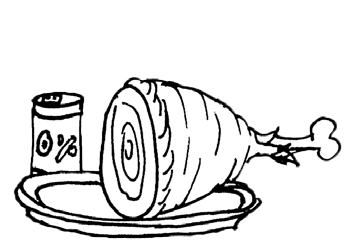
\includegraphics[height=20mm,right]{images/golonka.png}\vspace*{-21mm}\\
  Kolacja przy świecach - tylko ja i ona\\
  No może jeszcze polędwica smażona\\

  \hspace*{5mm}Golonka, golonka i piwo bezalkoholowe\\
  \\
  Nie mówię, że nie lubię klusek śląskich ze stekiem\\
  Ogórki kiszone zapijam kwaśnym mlekiem\\
  Ale gdy ona na boczku leży\\
  Wtedy gardzę nawet salcesonem świeżym\vspace*{2mm}
  \\
  Nie mówię, że nie lubię schabowych kotletów\\
  Albo na przykład rybnych filetów\\
  Lecz gdyby podano nawet grzyby ze śmietaną\\
  Albo kurczaki z rożna ja i tak z nią zostanę\\
\end{minipage}
\begin{minipage}[t]{0.13\textwidth}
  e a H$^7$\\
  e a H$^7$\\
  $\star$ e\\
  $\star$ H$^7$\vspace*{2mm}

  e a H$^7$\\
  e a H$^7$\\
  $\star$ e\\
  $\star$ H$^7$\\

  e a H$^7$\\

  e a H$^7$\\
  e a H$^7$\\
  $\star$ e\\
  $\star$ H$^7$\vspace*{2mm}

  e a H$^7$\\
  e a H$^7$\\
  $\star$ e\\
  $\star$ H$^7$\\

\end{minipage}
\begin{minipage}[t]{0.1\textwidth}
  ~\\
  \hspace*{-7mm} \chord{t}{n,p3,p4,p2,n,n}{$\star$}

\end{minipage}

% \newpage
\section{Goniąc kormorany}\textcolor{lightgray}{\textit{Piotr Szczepanik}}\vspace*{2mm}\\
\begin{minipage}[t]{0.78\textwidth}
  Dzień gaśnie w szarej mgle\\
  Wiatr strąca liście z drzew\\
  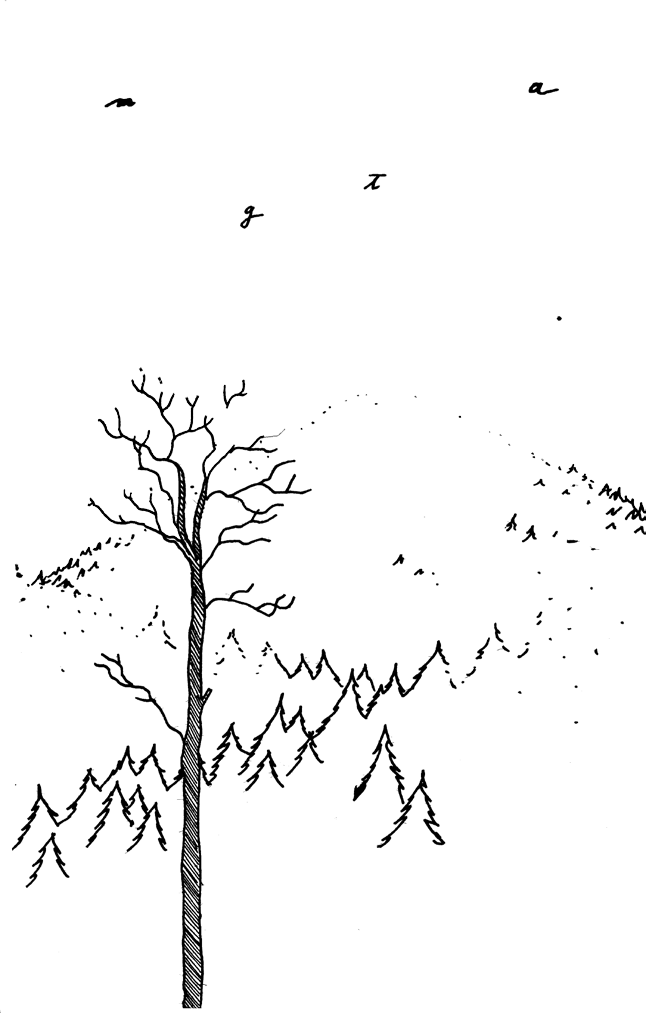
\includegraphics[height=72mm,right]{images/goniac_kormorany.png}\vspace*{-73mm}\\
  Sznur kormoranów w locie splątał się\\
  Pożegnał ciepły dzień\\
  Ostatni dzień w mazurskich stronach\\
  \hspace*{5mm}Zmierzch z jezior żagle zdjął\\
  \hspace*{5mm}Mgieł porozpinał splot\\
  \hspace*{5mm}Szmer tataraku jeszcze dobiegł nas\\
  \hspace*{5mm}Już wracać czas\\
  \\
  Noc się przybrała w czerń\\
  To smutny lata zmierzch\\
  Już kormorany odleciały stąd\\
  Poszukać ciepłych stron\\
  Powrócą z wiosną na jeziora\\
  \hspace*{5mm}Nikt nas nie żegna tu\\
  \hspace*{5mm}Dziś tak tu pusto już\\
  \hspace*{5mm}Mgły tylko ściga wśród sitowia wiatr\\
  \hspace*{5mm}Już wracać czas\\
\end{minipage}
\begin{minipage}[t]{0.22\textwidth}
  A h\\
  D E (EDEDE)\\
  A cis\\
  h\\
  A E\\
  A h\\
  D E (EDEDE)\\
  A cis\\
  h E A\\

  A h\\
  D E (EDEDE)\\
  A cis\\
  h\\
  A E\\
  A h\\
  D E (EDEDE)\\
  A cis\\
  h E A\\
\end{minipage}

\newpage
\section{Góralska opowieść}\textcolor{lightgray}{\textit{Babsztyl}}\\~\\
\begin{minipage}[t]{0.8\textwidth}
  Kiedy góral umiera, to góry z żalu sine\\
  Pochylają nad nim głowy, jak nad swoim synem\\
  Las w oddali szumi mu odwieczną pieśń bukową\\
  A on długo sposobi się przed najdalszą drogą\\
  \\
  Kiedy góral umiera, to nikt nad nim nie płacze\\
  Siedzi, czeka, aż kostucha w okno zakołacze\\
  Oczy jeszcze raz podniesie wysoko do nieba\\
  By pożegnać góry swoje, by im coś zaśpiewać\\

  \hspace*{5mm}Góry moje, wierchy moje, otwórzcie swe ramiona\\
  \hspace*{5mm}Niech na miękkim z mchu posłaniu cichuteńko skonam\\
  \hspace*{5mm}Ojcze mój, halny wietrze, powiej ku północy\\
  \hspace*{5mm}Ciepłą, drżącą swoją ręką zamknij zgasłe oczy\\
  \hspace*{5mm}Bym mógł w ziemię wrosnąć, strzelić potem\\
  \hspace*{5mm}Do słońca smreczyną\\
  \hspace*{5mm}I na zawsze szumieć już nad swoją dziedziną\\

  Kiedy góral umiera, to dzwony mu nie grają\\
  Cicho wspina się pod bramy góralskiego raju\\
  Tylko strumień na kamieniach żałobną nutę składa\\
  Tylko nocka chmurnooka górom opowiada\\

  A gdy góral już umrze, to nikt nie układa baśni\\
  Tylko w niebie roziskrzonym mała gwiazdka zgaśnie\\
  Ziemia twardą, szorstką ręką tuli go do siebie\\
  By na zawsze mógł już zostać pod góralskim niebem\\
\end{minipage}
\begin{minipage}[t]{0.2\textwidth}
  G G$^7$\\
  C G\\
  a C G\\
  a C G\\

  G G$^7$\\
  C G\\
  a C G\\
  a C G\\

  G a\\
  C G\\
  G a\\
  C G\\
  a\\
  C G\\
  a C G\\

  G G$^7$\\
  C G\\
  a C G\\
  a C G\\

  G G$^7$\\
  C G\\
  a C G\\
  a C G\\

\end{minipage}

\newpage
\section{Guaranteed}\textcolor{lightgray}{\textit{Eddie Vedder}}\\~\\
\begin{minipage}[t]{0.84\textwidth}
  On bended knee is no way to be free \\
  lifting up an empty cup I ask silently\\
  that all my destinations will accept the one that's me\\
  so I can breathe \\
  \\
  Circles they grow and they swallow people whole\\
  half their lives they say goodnight to wives they'll never know\\
  got a mind full of questions and a teacher in my soul \\
  so it goes... \\
  \\
  Don't come closer or I'll have to go\\
  Holding me like gravity are places that pull \\
  If ever there was someone to keep me at home \\
  It would be you...\\
  \\
  Everyone I come across in cages they bought\\
  they think of me and my wandering but I'm never what they thought \\
  got my indignation but I'm pure in all my thoughts \\
  I'm alive... \\
  \\
  Wind in my hair, I feel part of everywhere \\
  underneath my being is a road that disappeared \\
  late at night I hear the trees they're singing with the dead \\
  overhead... \\
  \\
  Leave it to me as I find a way to be \\
  consider me a satellite forever orbiting \\
  I knew all the rules but the rules did not know me \\
  guaranteed...\\
  \\

\end{minipage}
\begin{minipage}[t]{0.16\textwidth}
  G h\\
  G$^7$ C\\
  C G\\
  D (D$^2$D$^4$D$^5$)\\

  G h\\
  G$^7$ C\\
  C G\\
  D (D$^2$D$^4$D$^5$)\\

  G h\\
  G$^7$ C\\
  C G\\
  D (D$^2$D$^4$D$^5$)\\

  G h\\
  G$^7$ C\\
  C G\\
  D (D$^2$D$^4$D$^5$)\\

  G h\\
  G$^7$ C\\
  C G\\
  D (D$^2$D$^4$D$^5$)\\

  G h\\
  G$^7$ C\\
  C G\\
  D (D$^2$D$^4$D$^5$)\\
\end{minipage}

\newpage
\section{Hallelujah}\textcolor{lightgray}{\textit{Leonard Cohen}}\\~\\
\begin{minipage}[t]{0.8\textwidth}
  I've heard there was a secret chord\\
  That David played and it pleased the Lord\\
  But you don't really care for music, do you?\\
  It goes like this, the fourth, the fifth\\
  The minor fall, the major lift\\
  The baffled king composing Hallelujah\\
  \\
  \hspace*{6mm}Hallelujah (x4)\\
  \\
  Your faith was strong, but you needed proof\\
  You saw her bathing on the roof\\
  Her beauty in the moonlight overthrew you\\
  She tied you to a kitchen chair\\
  She broke your throne and she cut your hair\\
  And from your lips she drew the Hallelujah\\
  \\
  Baby I've been here before\\
  I know this room, I've walked this floor\\
  I used to live alone before I knew you\\
  I've seen your flag on the Marble Arch\\
  Love is not a victory march\\
  It's a cold and it's a broken Hallelujah\\
  \\
  There was a time you let me know\\
  What's really going on below\\
  But now you never show it to me, do you?\\
  I remember when I moved in you\\
  The holy dove was moving too\\
  And every breath we drew was Hallelujah\\
  \\
  Maybe there's a God above,\\
  And all I've ever learned from love\\
  Was how to shoot at someone who outdrew you\\
  It's not a cry you can hear at night\\
  It's not somebody who's seen the light\\
  It's a cold and it's a broken Hallelujah\\
  \\
  You say I took the name in vain\\
  I do not even know the name\\
  But if I did, well really, what's it to you?\\
  There's a blaze of light in every word\\
  It doesn't matter which you heard\\
  The holy or the broken Hallelujah\\
\end{minipage}
\begin{minipage}[t]{0.2\textwidth}
  A fis\\
  A fis\\
  D E A (E)\\
  A D E\\
  fis D\\
  E cis fis\\

  D fis D A E A (E)\\

  A fis\\
  A fis\\
  D E A (E)\\
  A D E\\
  fis D\\
  E cis fis\\

  A fis\\
  A fis\\
  D E A (E)\\
  A D E\\
  fis D\\
  E cis fis\\

  A fis\\
  A fis\\
  D E A (E)\\
  A D E\\
  fis D\\
  E cis fis\\

  A fis\\
  A fis\\
  D E A (E)\\
  A D E\\
  fis D\\
  E cis fis\\

  A fis\\
  A fis\\
  D E A (E)\\
  A D E\\
  fis D\\
  E cis fis\\
\end{minipage}
\newpage
\begin{minipage}[t]{0.8\textwidth}

  \hspace*{6mm}Hallelujah (x4)\\

  I did my best, it wasn't much\\
  I couldn't feel, so I tried to touch\\
  I've told the truth, I didn't come to fool you\\
  And even though it all went wrong\\
  I'll stand before the Lord of Song\\
  With nothing on my tongue but Hallelujah\\
\end{minipage}
\begin{minipage}[t]{0.2\textwidth}

  D fis D A E A (E)\\

  A fis\\
  A fis\\
  D E A (E)\\
  A D E\\
  fis D\\
  E cis fis\\
\end{minipage}

% \newpage
\section{Hanko}\textcolor{lightgray}{\textit{Stanisław Grzesiuk}}\\~\\
\begin{minipage}[t]{0.8\textwidth}
  Apaszem Staszek był, w krąg znały go ulice\\
  W spelunkach ciemnych, gdzie podłe życie wre\\
  Kochanką jego była zwykła ulicznica\\
  Co gdzieś na rogu sprzedawała ciało swe\\
  Pomimo to Stach kochał swoją Hankę\\
  Choć nieraz zbił, skatował aż do krwi\\
  Lecz kiedy znów przepraszał swą bogdankę\\
  No to tak do niej szeptał czułe słowa te\\
  \\
  \hspace*{5mm}Hanko, o tobie marzę wśród bezsennych nocy\\
  \hspace*{5mm}Hanko, ja bez ciebie nie potrafię żyć\\
  \hspace*{5mm}Wciąż bym się tylko wpatrywał w twoje oczy\\
  \hspace*{5mm}I przy twym boku ja tylko chciałbym być\\
  \\
  \hspace*{5mm}Hanko, twe ciało słodko pręży się, przegin\\
  \hspace*{5mm}Hanko, daj usta niech przeminie ból i żal\\
  \hspace*{5mm}Że w oczach łzy, to wiem, że moja wina\\
  \hspace*{5mm}Że życie płynie wśród tak burzliwych fal\\
  \\
  Gdy Stach dowiedział się, że Hanka go zdradziła\\
  To się roześmiał swym okrutnym ha, ha, ha\\
  W spelunkach, tam, gdzie granda wódkę piła\\
  I Staszek pił, choć serce z bólu łka\\
  Po roku znów Stach spotkał swoją Hankę\\
  I w ręku błysnął długi, ostry nóż\\
  I nożem w serce pchnął swoją bogdankę\\
  A nad jej trupem szeptał: Cóż jam zrobił, cóż?\\
\end{minipage}
\begin{minipage}[t]{0.2\textwidth}
  a E\\
  E a\\
  a E\\
  E a\\
  A d\\
  G  C (E)\\
  a E\\
  E  a (E a)\\
  \\
  a E\\
  E a\\
  a E\\
  E a\\

  a E\\
  E a\\
  a E\\
  E a\\

  a E\\
  E a\\
  a E\\
  E a\\
  A d\\
  G  C (E)\\
  a E\\
  E  a (E a)\\
\end{minipage}

\newpage
\section{Have you ever seen the rain}\textcolor{lightgray}{\textit{Creedence Clearwater Revival}}\\~\\
\begin{minipage}[t]{0.7\textwidth}
  Someone told me long ago\\
  There's a calm before the storm\\
  I know, it's been comin' for some time\\
  When it's over, so they say\\
  It'll rain on a sunny day\\
  I know, shining down like water\\
  \\
  I wanna know, have you ever seen the rain?\\
  I wanna know, have you ever seen the rain\\
  Comin' down on a sunny day?\\
  \\
  Yesterday and days before\\
  Sun is cold and rain is hard\\
  I know, been that way for all my time\\
  'Til forever on it goes\\
  Through the circle, fast and slow\\
  I know, it can't stop, I wonder\\
\end{minipage}
\begin{minipage}[t]{0.3\textwidth}
  C\\ C\\
  G C\\
  C\\ C\\
  G C\\

  F G C a\\
  F G C a\\
  F G C\\

  C\\ C\\
  G C\\
  C\\ C\\
  G C\\
\end{minipage}

% \newpage
\section{Hawiarska Koliba}\textcolor{lightgray}{\textit{Wiesław Witek}}\\~\\
\begin{minipage}[t]{0.8\textwidth}
  Już księżyc na niebo wychodzi\\
  Zapłoną dokoła ogniska\\
  I wkrótce popłynie z Hawiarskiej Koliby\\
  Melodia nam wszystkim tak bliska\\
  \\
  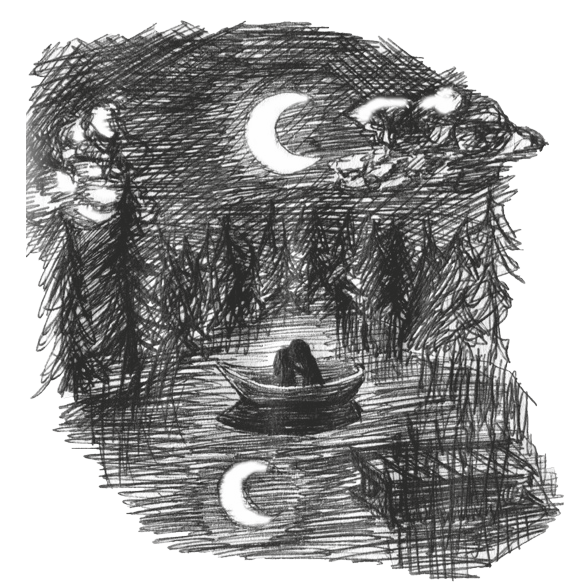
\includegraphics[width = 40mm, right]{images/hawiarska_koliba.png}\vspace*{-41.5mm}\\
  Usiadła już brać rozśpiewana\\
  Dokoła złotego ogniska\\
  Wiatr niesie melodię z Hawiarskiej Koliby\\
  Nad pola, nad lasy, nad urwiska\\
  \\
  Zaniesie wiatr naszą melodię\\
  Do domów Wołochów i Łemków\\
  Piosenkę rajdową z Hawiarskiej Koliby\\
  Piosenkę wrocławskich włóczęgów\\
  \\
  Już księżyc blednie na niebie\\
  I słońca promień już błyska\\
  Pogasły ogniska w Hawiarskiej Kolibie\\
  Do snu kładzie się cała izba\\
\end{minipage}
\begin{minipage}[t]{0.2\textwidth}
  C G C C$^7$\\
  F G C C$^7$\\
  F G C a\\
  F G C (C$^7$)\\

  C G C C$^7$\\
  F G C C$^7$\\
  F G C a\\
  F G C (C$^7$)\\

  C G C C$^7$\\
  F G C C$^7$\\
  F G C a\\
  F G C (C$^7$)\\

  C G C C$^7$\\
  F G C C$^7$\\
  F G C a\\
  F G C (C$^7$)\\
\end{minipage}
% ~\\~\\~\\


\newpage
\section{Hej przyjaciele}\textcolor{lightgray}{\textit{Babsztyl}}\\~\\
\begin{minipage}[t]{0.75\textwidth}
  Tam, dokąd chciałem, już nie dojdę, szkoda zdzierać nóg\\
  Już wędrówki naszej wspólnej nadchodzi kres\\
  Wy pójdziecie inną drogą, zostawicie mnie\\
  Odejdziecie, sam zostanę na rozstaju dróg\\
  \\
  \hspace*{5mm}Hej, przyjaciele, zostańcie ze mną\\
  \hspace*{5mm}Przecież wszystko to, co miałem, oddałem wam\\
  \hspace*{5mm}Hej, przyjaciele, choć chwilę jedną\\
  \hspace*{5mm}Znowu w życiu mi nie wyszło, znowu będę sam\\
  \\
  Znów spóźniłem się na pociąg i odjechał już\\
  Tylko jego mglisty koniec zamajaczył mi\\
  Stoję smutny na peronie z tą walizką jedną\\
  Tak jak człowiek, który zgubił od domu swego klucz\\
  \\
  Tam, dokąd chciałem, już nie dojdę, szkoda zdzierać nóg\\
  Już wędrówki naszej wspólnej nadchodzi kres\\
  Wy pójdziecie inną drogą, zostawicie mnie\\
  Zamazanych drogowskazów nie odczytam już\\
\end{minipage}
\begin{minipage}[t]{0.25\textwidth}
  C G F C\\
  C G F G C\\
  C G F C\\
  C G F G C\\

  C G (G/Fis/F) F C\\
  C G F G C\\
  C G (G/Fis/F) F C\\
  C G F G C\\

  C G F C\\
  C G F G C\\
  C G F C\\
  C G F G C\\

  C G F C\\
  C G F G C\\
  C G F C\\
  C G F G C\\

\end{minipage}

\newpage
\section{Hej w góry}\textcolor{lightgray}{\textit{}}\\~\\
\begin{minipage}[t]{0.9\textwidth}
  Zagrajcie nam, może się cofnie czas\\
  Do tamtych dni z naszych marzeń\\
  Do dni spędzonych pośród sennych skał\\
  Gdy czas upływał w pełni zdarzeń\\
  \\
  \hspace*{3mm}Hej w góry, w góry, w góry, popatrz, tam wstaje blady świt\\
  \hspace*{3mm}Jeszcze tak nieporadnie chce ominąć szczyt\\
  \hspace*{3mm}Hej, miły panie, czekaj, zaraz my też będziemy tam\\
  \hspace*{3mm}Nie będziesz musiał schodzić z połoniny sam, z połoniny sam\\
  \\
  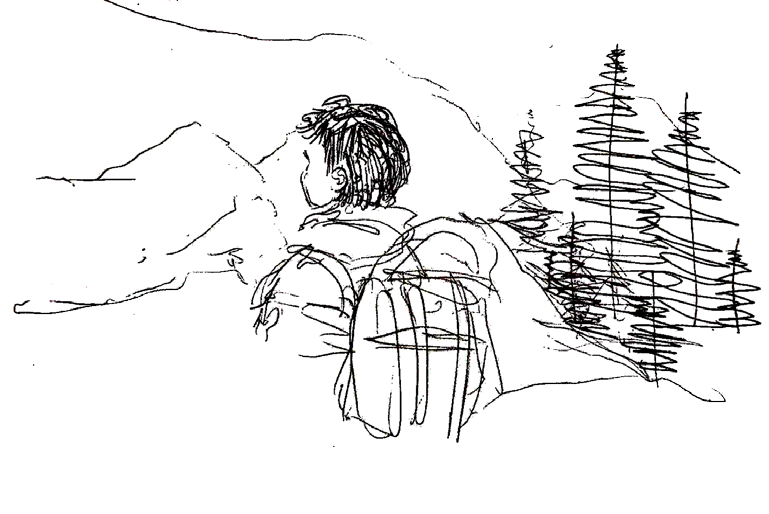
\includegraphics[height=40mm, right]{images/hej_w_gory.png}\vspace*{-40mm}\\
  Bywały dni, że słońca złoty blask\\
  W zawody szedł z sennym brzaskiem\\
  To dziwne więc, że dzisiaj skoro świt\\
  I wiatr, i deszcz razem tańczą\\
  \\
  Muzyka gór moją miłością jest\\
  Upaja mnie zapach lasu\\
  Potoków szum, leśnych ptaków śpiew\\
  Wspomnieniem są lepszych czasów\\
  \\
  Zagrajcie mi, może się spełni czas\\
  I znów poczuję dym ogniska\\
  Namiotów krąg ujrzę w oddali gdzieś\\
  I znów będziemy razem wszyscy\\
\end{minipage}
\begin{minipage}[t]{0.1\textwidth}
  C d\\
  F C G\\
  C d\\
  F C G\\

  C d\\
  F C G\\
  C d\\
  F C G\\

  C d\\
  F C G\\
  C d\\
  F C G\\

  C d\\
  F C G\\
  C d\\
  F C G\\

  C d\\
  F C G\\
  C d\\
  F C G\\
\end{minipage}

\newpage
\section{Hey Jude}\textcolor{lightgray}{\textit{The Beatles}}\\~\\
\begin{minipage}[t]{0.8\textwidth}
  Hey Jude, don't make it bad.\\
  Take a sad song and make it better.\\
  Remember to let her into your heart,\\
  Then you can start to make it better.\\
  \\
  Hey Jude, don't be afraid.\\
  You were made to go out and get her.\\
  The minute you let her under your skin,\\
  Then you begin to make it better.\\
  \\
  \hspace*{4mm}And anytime you feel the pain, hey Jude, refrain,\\
  \hspace*{4mm}Don't carry the world upon your shoulders.\\
  \hspace*{4mm}For well you know that it's a fool who plays it cool\\
  \hspace*{4mm}By making his world a little colder.\\
  \\
  Hey Jude, don't let me down.\\
  You have found her, now go and get her.\\
  Remember to let her into your heart,\\
  Then you can start to make it better.\\
  \\
  \hspace*{4mm}So let it out and let it in, hey Jude, begin,\\
  \hspace*{4mm}You're waiting for someone to perform with.\\
  \hspace*{4mm}And don't you know that it's just you, hey Jude, you'll do,\\
  \hspace*{4mm}The movement you need is on your shoulder.\\
  \\
  Hey Jude, don't make it bad.\\
  Take a sad song and make it better.\\
  Remember to let her under your skin,\\
  Then you'll begin to make it\\
  \\
  Better better better better better better, oh.\\
  Na na na nananana, nannana, hey Jude...\\
  \hspace*{23mm}\textit{\footnotesize(repeat X number of times, fade)}\\
\end{minipage}
\begin{minipage}[t]{0.2\textwidth}
  A E\\E$^7$ A\\D A\\E E$^7$ A\\

  A E\\E$^7$ A\\D A\\E E$^7$ A\\

  A$^7$ D fis h\\D E$^7$ A\\A$^7$ D fis h\\D E$^7$ A (A$^7$ E$^7$)\\

  A E\\E$^7$ A\\D A\\E E$^7$ A\\

  A$^7$ D fis h\\D E$^7$ A\\A$^7$ D fis h\\D E$^7$ A (A$^7$ E$^7$)\\

  A E\\E$^7$ A\\D A\\E E$^7$ A\\

  ~\\
  A G D A\\

\end{minipage}

\newpage
\section{Highway to hell}\textcolor{lightgray}{\textit{AC/DC}}\\~\\
\begin{minipage}[t]{0.8\textwidth}
  Living easy, living free, season ticket on a one-way ride\\
  Asking nothing, leave me be, taking everything in my stride\\
  Don't need reason, don't need rhyme, ain't nothing I would rather do\\
  Going down, party time, my friends are gonna be there too\\
  \\
  \hspace*{5mm}I'm on the highway to hell\hspace*{10mm}$/ \times$4\\
  \\
  No stop signs, speed limit, nobody's gonna slow me down\\
  Like a wheel, gonna spin it, nobody's gonna mess me around\\
  Hey Satan, paid my dues playing in a rocking band\\
  Hey mama, look at me, I'm on my way to the promised land\\

  \hspace*{10mm}Don't stop me
\end{minipage}
\begin{minipage}[t]{0.2\textwidth}
  A |D/fis G| A\\~\\~\\~\\
  (E)\\
  A D (G D)\\

  A |D/fis G| A\\~\\~\\~\\
  (E)\\
\end{minipage}
\vspace*{2cm}\\
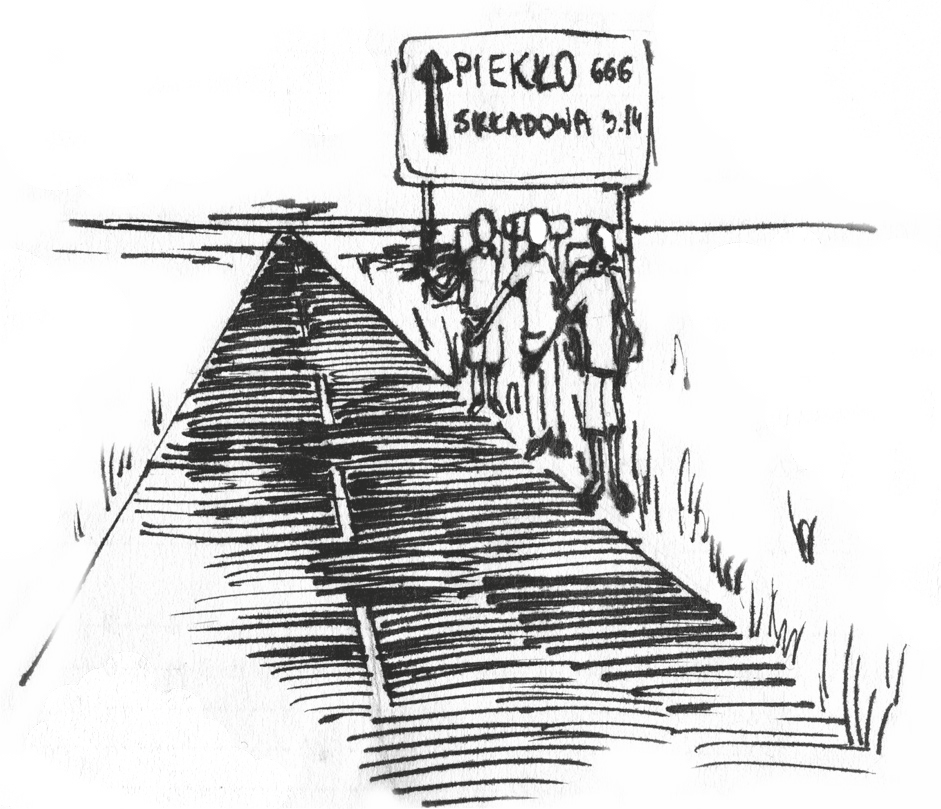
\includegraphics[width=0.7\textwidth, center]{images/highway_to_hell.png}\\

\newpage
\section{Historia jednej znajomości}\textcolor{lightgray}{\textit{Czerwone Gitary}}\\~\\
\begin{minipage}[t]{0.8\textwidth}
  Morza szum, ptaków śpiew, złota plaża pośród drzew\\
  Wszystko to w letnie dni przypomina Ciebie mi\\
  Przypomina Ciebie mi\\
  \\
  \hspace*{5mm}Sia la la la la…\\
  \\
  Szłaś przez skwer, z tyłu pies Głos Wybrzeża w pysku niósł\\
  Wtedy to pierwszy raz uśmiechnęłaś do mnie się\\
  Uśmiechnęłaś do mnie się\\
  \\
  Odtąd już dzień po dniu upływały razem nam\\
  Rano skwer, plaża lub molo, gdy zapada zmierzch\\
  Molo, gdy zapada zmierzch\\
  \\
  Płynął czas, letni czas, aż wakacji nadszedł kres\\
  Przyszedł dzień, w którym już rozstać musieliśmy się\\
  Rozstać musieliśmy się\\
\end{minipage}
\begin{minipage}[t]{0.2\textwidth}
  a F aEa\\
  C d\\
  a F E\\
  \\
  a d E\\

  a F aEa\\
  C d\\
  a F E\\

  a F aEa\\
  C d\\
  a F E\\

  a F aEa\\
  C d\\
  a F E\\
\end{minipage}
\vspace*{2cm}\\
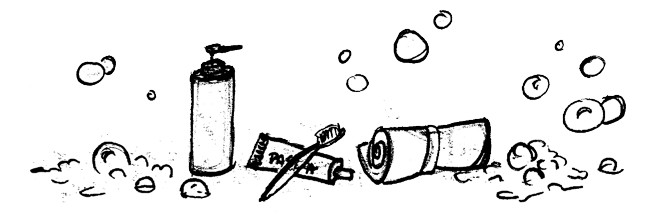
\includegraphics[width = 0.7\textwidth, center]{images/historia_jednej_znajomosci.png}\\

\newpage
\section{Hotel California}\textcolor{lightgray}{\textit{Eagles}}\vspace*{2mm}\\
\begin{minipage}[t]{0.9\textwidth}
  On a dark desert highway, cool wind in my hair\\
  Warm smell of colitas rising up through the air\\
  Up ahead in the distance I saw a shimmering light\\
  My head grew heavy and my sight grew dim\\
  I had to stop for the night\vspace*{2mm}\\
  There she stood in the doorway; I heard the mission bell\\
  And I was thinking to myself, This could be heaven or this could be hell\\
  Then she lit up a candle and she showed me the way\\
  There were voices down the corridor\\
  I thought I heard them say\vspace*{2mm}\\
  \hspace*{5mm}Welcome to the Hotel California\\
  \hspace*{5mm}Such a lovely place, such a lovely face\\
  \hspace*{5mm}Plenty of room at the Hotel California\\
  \hspace*{5mm}Any time of year you can find it here\vspace*{2mm}\\
  Her mind is Tiffany-twisted, she got the Mercedes-Benz\\
  She got a lot of pretty, pretty boys she calls friends\\
  How they dance in the courtyard, sweet summer sweat\\
  Some dance to remember\\
  Some dance to forget\vspace*{2mm}\\
  So I called up the captain, Please bring me my wine\\
  He said, We haven't had that spirit here since nineteen sixty nine\\
  And still those voices are calling from far away\\
  Wake you up in the middle of the night\\
  Just to hear them say\vspace*{2mm}\\
  \hspace*{5mm}Welcome to the Hotel California\\
  \hspace*{5mm}Such a lovely place such a lovely face\\
  \hspace*{5mm}They livin' it up at the Hotel California\\
  \hspace*{5mm}What a nice surprise bring your alibis\vspace*{2mm}\\
  Mirrors on the ceiling, the pink champagne on ice\\
  And she said, We are all just prisoners here, of our own device\\
  And in the master's chambers, they gathered for the feast\\
  They stab it with their steely knives\\
  But they just can't kill the beast\vspace*{2mm}\\
  Last thing I remember, I was running for the door\\
  I had to find the passage back to the place I was before\\
  Relax, said the night man, we're programmed to receive\\
  You can check-out any time you like\\
  But you can never leave!\\
\end{minipage}
\begin{minipage}[t]{0.2\textwidth}
  h Fis\\
  A E\\
  G D\\
  e\\
  Fis\vspace*{2mm}\\
  h Fis\\
  A E\\
  G D\\
  e\\
  Fis\vspace*{2mm}\\
  G D\\
  Fis h\\
  G D\\
  e Fis\vspace*{2mm}\\
  h Fis\\
  A E\\
  G D\\
  e\\
  Fis\vspace*{2mm}\\
  h Fis\\
  A E\\
  G D\\
  e\\
  Fis\vspace*{2mm}\\
  G D\\
  Fis h\\
  G D\\
  e Fis\vspace*{2mm}\\
  h Fis\\
  A E\\
  G D\\
  e\\
  Fis\vspace{1.5mm}\\
  h Fis\\
  A E\\
  G D\\
  e\\
  Fis\\
\end{minipage}

\newpage
\section{House of the Rising Sun}\textcolor{lightgray}{\textit{The Animals}}\\~\\
\begin{minipage}[t]{0.8\textwidth}
  There is a house in New Orleans\\
  They call the Rising Sun\\
  And it's been the ruin of many a poor boy\\
  And God I know I'm one\\
  \\
  My mother was a tailor\\
  She sewed my new blue jeans\\
  My father was a gamblin' man\\
  Down in New Orleans\\
  \\
  Now the only thing a gambler needs\\
  Is a suitcase and a trunk\\
  And the only time he'll be satisfied\\
  Is when he's all a-drunk\\
  \\
  Oh mother, tell your children\\
  Not to do what I have done\\
  Not to spend your lives in sin and misery\\
  In the house of the Rising Sun\\
  \\
  I've got one foot on the platform\\
  The other foot on the train\\
  I'm going back to New Orleans\\
  To wear that ball and chain\\

\end{minipage}
\begin{minipage}[t]{0.2\textwidth}
  a C D F\\
  a C E E$^7$\\
  a C D F\\
  a E a (E)\\

  a C D F\\
  a C E E$^7$\\
  a C D F\\
  a E a (E)\\

  a C D F\\
  a C E E$^7$\\
  a C D F\\
  a E a (E)\\

  a C D F\\
  a C E E$^7$\\
  a C D F\\
  a E a (E)\\

  a C D F\\
  a C E E$^7$\\
  a C D F\\
  a E a (E)\\
\end{minipage}

\newpage
\section{Huśtawki}\textcolor{lightgray}{\textit{Jacek Kleyff / Kwiat Jabłoni}}\vspace*{2mm}\\
\begin{minipage}[t]{0.85\textwidth}
  A czy przyroda, kolebka, myślała kiedyś dokładnie\\
  Na co jej wielkie mamuty? Ani wygląda to ładnie\\
  I ani z nich skóra na buty \vspace*{2mm}
  \\
  Nie ma co pytać, koledzy - robiła i tak jej wyszło\\
  Nikt nie wymyślał specjalnie, tego w czym żyć nam przyszło\\
  Uprzedzam o tym lojalnie\\
  \\
  \hspace*{5mm}Jeden jest rytm, jeden rytm, jeden jest wydech i wdech\\
  \hspace*{5mm}Nasyć się równym oddechem, nasyć się dzisiaj za trzech, bo\\
  \hspace*{5mm}Raz tylko dany Ci czas i ani on Twój ani czyj\\
  \hspace*{5mm}Z czasem się wszystko ustoi, więc żyj na huśtawce, żyj\\
  \\
  Nie skacz tak zaraz na szyny, jeszcze nie o tę grasz stawkę\\
  W wesołym miasteczku dziewczyny chcą z Tobą iść na huśtawkę\\
  Lepiej Ci będzie z nimi \vspace*{2mm}

  Pachnie tak mocno siano, kwiaty się gną od motyli\\
  Jeździ słonko po niebie, światło ucieka ślad myli\\
  Miasteczko czeka na Ciebie\\
  \\
  \hspace*{7mm}Jeden jest rytm, jeden rytm...\vspace*{2mm}
  \\
  \hspace*{5mm}I jeden jest rytm, jeden rytm, jeden jest węgiel i tlen\\
  \hspace*{5mm}Zwykłą losu koleją, praca, posiłek i sen\\
  \hspace*{5mm}I jeden przypada na dzień, świt jeden i jeden zmrok\\
  \hspace*{5mm}Pierwsi się łudzą nadzieją, a drudzy równają krok\\
\end{minipage}
\begin{minipage}[t]{0.15\textwidth}
  A E\\
  fis D\\
  A E \vspace*{2mm}

  A E\\
  fis D\\
  A E\\

  A E\\
  fis D\\
  A E\\
  fis D\\

  A E\\
  fis D\\
  A E \vspace*{2mm}

  A E\\
  fis D\\
  A E\\
  \\
  ~ \vspace*{2mm}
  \\
  A E\\
  fis D\\
  A E\\
  fis D\\
\end{minipage}
% \begin{minipage}[t]{0.2\textwidth}
% D A\\
% h G\\
% D A\\

% D A\\
% h G\\
% D A\\

% D A\\
% h G\\
% D A\\
% h G\\

% D A\\
% h G\\
% D A\\

% D A\\
% h G\\
% D A\\

% ~\\

% D A\\
% h G\\
% D A\\
% h G\\
% \end{minipage}

% \newpage
\section{I am sailing}\textcolor{lightgray}{\textit{Rod Stewart
  }}\vspace*{2mm}\\
\begin{minipage}[t]{0.80\textwidth}
  I am sailing, I am sailing home again 'cross the sea\\
  I am sailing stormy waters to be near you, to be free\vspace*{2mm}
  \\
  I am flying, I am flying like a bird 'cross the sky\\
  I am flying passing high clouds to be with you, to be free\\
  \\
  \hspace*{5mm}Can you hear me, can you hear me \\
  \hspace*{5mm}through the dark night far away?\\
  \hspace*{5mm}I am dying, forever crying \\
  \hspace*{5mm}to be with you, who can say\\
  \\
  We are sailing, we are sailing home again 'cross the sea\\
  We are sailing stormy waters to be near you, to be free\\
\end{minipage}
\begin{minipage}[t]{0.2\textwidth}
  C a F C\\
  d a d G C (G)\vspace*{2mm}

  C a F C\\
  d a d G C (G)\\

  C a\\ F C\\
  d a d\\ G C (G)\\

  C a F C\\
  d a d G C (G)\\
  G d C\\
\end{minipage}

\newpage
\section{I can't help falling in love}\textcolor{lightgray}{\textit{Elvis Presley}}\\~\\
\begin{minipage}[t]{0.8\textwidth}
  ~\\
  Wise men say, only fools rush in\\
  But I can't help falling in love with you\vspace*{1.8mm}

  Shall I stay, Would it be a sin\\
  If I can't help falling in love with you?\\

  \hspace*{5mm}Like a river flows\\
  \hspace*{5mm}Surely to the sea\\
  \hspace*{5mm}Darling, so it goes\\
  \hspace*{5mm}Some things are meant to be\\

  Take my hand, take my whole life, too\\
  For I can't help falling in love with you\\
  ~\\
  ~\\
\end{minipage}
\begin{minipage}[t]{0.2\textwidth}
  (C G C G)\\
  C e a a, F C G G\\
  F G a F, C G C C\vspace*{1.8mm}

  C e a a, F C G G\\
  F G a F, C G C C\\

  e H$^7$\\
  e H$^7$\\
  e H$^7$\\
  e A$^7$ d G\\

  C e a a, F C G G\\
  F G a F, C G C C\\

\end{minipage}

% \newpage
\section{I shall be released}\textcolor{lightgray}{\textit{Bob Dylan}}\\~\\
\begin{minipage}[t]{0.8\textwidth}
  They say everything can be replaced\\
  Yet every distance is not near\\
  So I remember every face\\
  Of every man who put me here\\
  \\
  \hspace*{5mm}I see my light come shining \\
  \hspace*{5mm}From the west unto the east\\
  \hspace*{5mm}Any day now, any day now\\
  \hspace*{5mm}I shall be released\\
  \\
  They say every man needs protection\\
  They say every man must fall\\
  Yet I swear I see my reflection\\
  Some place so high above this wall\\
  \\
  Standing next to me in this lonely crowd\\
  Is a man who swears he's not to blame\\
  All day long I hear him shout so loud\\
  Crying out that he's been framed\\
\end{minipage}
\begin{minipage}[t]{0.2\textwidth}
  A h\\
  (c) cis E A\\
  A h\\
  (c) cis E A\\

  A h\\
  (c) cis E A\\
  A h\\
  (c) cis E A\\

  A h\\
  (c) cis E A\\
  A h\\
  (c) cis E A\\

  A h\\
  (c) cis E A\\
  A h\\
  (c) cis E A\\

\end{minipage}

\newpage
\section{Imagine}\textcolor{lightgray}{\textit{John Lennon}}\\~\\
\begin{minipage}[t]{0.65\textwidth}
  Imagine there's no heaven\\
  It's easy if you try\\
  No hell below us\\
  Above us, only sky\\
  Imagine all the people\\
  Livin' for today\\
  \\
  Imagine there's no countries\\
  It isn't hard to do\\
  Nothing to kill or die for\\
  And no religion, too\\
  Imagine all the people\\
  Livin' life in peace\\
  \\
  \hspace*{5mm}You may say I'm a dreamer\\
  \hspace*{5mm}But I'm not the only one\\
  \hspace*{5mm}I hope someday you'll join us\\
  \hspace*{5mm}And the world will be as one\\

  Imagine no possessions\\
  I wonder if you can\\
  No need for greed or hunger\\
  A brotherhood of man\\
  Imagine all the people\\
  Sharing all the world\\
  \\
  \hspace*{5mm}You may say I'm a dreamer...\\
\end{minipage}
\begin{minipage}[t]{0.35\textwidth}
  C C$^{7+}$ F\\
  C C$^{7+}$ F\\
  C C$^{7+}$ F\\
  C C$^{7+}$ F\\
  F a d$^7$ d (d$^\star$)\\
  G G$^7$\\

  C C$^{7+}$ F\\
  C C$^{7+}$ F\\
  C C$^{7+}$ F\\
  C C$^{7+}$ F\\
  F a d$^7$ d (d$^\star$)\\
  G G$^7$\\

  F G C (C$^{7+}$) E$^7$\\
  F G C (C$^{7+}$) E$^7$\\
  F G C (C$^{7+}$) E$^7$\\
  F G C\\

  C C$^{7+}$ F\\
  C C$^{7+}$ F\\
  C C$^{7+}$ F\\
  C C$^{7+}$ F\\
  F a d$^7$ d (d$^\star$)\\
  G G$^7$\\
  \chords{
    \hspace*{-2cm}\vspace*{-2cm}
  \chord{t}{n,p3,p2,n,n,n}{{\small C$^{7+}$}} 
  \chord{t}{n,3,n,2,3,1}{{\small d$^\star$}}
  }
\end{minipage}

\newpage
\section{Ja mam tylko jeden świat}\textcolor{lightgray}{\textit{}}\\~\\
\begin{minipage}[t]{0.9\textwidth}
  Kiedy w piątek słońce świeci, serce mi do góry wzlata\\
  Bo w sobotę wezmę plecak w podróż do mojego świata\\
  \\
  \hspace*{5mm}Bo ja mam tylko jeden świat\\
  \hspace*{5mm}Słońce, góry, pola, wiatr (hej, pola, wiatr)\\
  \hspace*{5mm}I nic mnie więcej nie obchodzi\\
  \hspace*{5mm}Bom turystą się urodził\\
  \\
  Dla mnie w mieście jest za ciasno, wśród pojazdów, kurzu, spalin\\
  Ja w zieloną jadę ciszę, w ścieżki pełne słodkich malin\\
  \\
  Myślę, leżąc pośród kwiatów, czy w jęczmienia złotym łanie\\
  Czy przypadkiem za pół wieku coś z tym światem się nie stanie\\
  \\
  Chciałbym, żeby ten mój świat przetrwał jeszcze z tysiąc lat\\
  Żeby mogły nasze dzieci z tego świata też się cieszyć\\
\end{minipage}
\begin{minipage}[t]{0.2\textwidth}
  e A$^7$ D\\
\end{minipage}

% \newpage
\section{Jak malowany ptak}\textcolor{lightgray}{\textit{Dżem}}\\~\\
\begin{minipage}[t]{0.8\textwidth}
  Za oknem żywi ludzie, inny wymiar, inne życie\\
  Czy wiesz, jak ciężko jest walczyć z każdym nowym dniem?\\
  Każdej nocy modlić się o bezpieczny, spokojny sen\\
  Bez nadziei i bez szans spojrzeć w karty mówiąc, "Pas"\\

  \hspace*{5mm}Czy przyjmiesz mnie mój Boże\\
  \hspace*{5mm}Kiedy odejść przyjdzie czas?\\
  \hspace*{5mm}Czy podasz mi swą rękę?\\
  \hspace*{5mm}A może będziesz się bał\\
  \hspace*{5mm}Będziesz się bał\\

  Za oknem wrzeszczą ludzie, szybę stłukł rzucony kamień\\
  Czy wiesz, jak czuję się gdy w objęciach trzymam śmierć?\\
  Gdy wyrok napisany w lekarza oczach szklanych\\
  Gdy lecą, lecą tak, jak ten malowany ptak\\

  Czy przyjmiesz mnie, mój Boże...\\

\end{minipage}
\begin{minipage}[t]{0.2\textwidth}
  a C D$^7$ F$^{7+}$\\
  a C D$^7$ F$^{7+}$\\
  a C D$^7$ F$^{7+}$\\
  a C D$^7$ F$^{7+}$\\

  a e\\
  F$^{7+}$ G\\
  a e\\
  F$^{7+}$ G\\
  (a C D$^7$ F$^{7+}$)\\

  a C D$^7$ F$^{7+}$\\
  a C D$^7$ F$^{7+}$\\
  a C D$^7$ F$^{7+}$\\
  a C D$^7$ F$^{7+}$\\
\end{minipage}

\newpage
\section{Jaka jesteś}\textcolor{lightgray}{\textit{Tomasz Lewandowski}}\\~\\
\begin{minipage}[t]{0.7\textwidth}
  Jesteś bitwą moją nieskończoną\\
  W której ciągle o przyczółek walczę\\
  Jesteś drzwiami, które otworzyłem\\
  A potem przycięły mi palce\\

  \hspace*{5mm} Jesteś kartką z kalendarza\\
  \hspace*{5mm} Zagubioną gdzieś pomiędzy szufladami\\
  \hspace*{5mm} I ulicą, na której co dzień\\
  \hspace*{5mm} Uciekałem między latarniami\\

  Jesteś mgłą ogromną, niezmierzoną\\
  Ciszą w huku i łoskotem ciszy\\
  Jesteś piórem i wyblakłą kartką\\
  Którym i na której dzisiaj piszę\\

  Przyszłaś do mnie, a ja nie spostrzegłem\\
  Dziś już tylko mogę mówić - byłaś\\
  Nie wiem, czy na jawie wzięłaś mnie za rękę\\
  Czy, jak wszystko, ty się tylko śniłaś\\

\end{minipage}
\begin{minipage}[t]{0.3\textwidth}
  G a\\
  C D G (a C D) \\
  G a\\
  C D G (a C D) \\

  G a\\
  C D G (a C D) \\
  G a\\
  C D G (a C D) \\

  G a\\
  C D G (a C D) \\
  G a\\
  C D G (a C D) \\

  G a\\
  C D G (a C D) \\
  G a\\
  C D G (a C D) \\

\end{minipage}

% \newpage
\section{Jaki był ten dzień}\textcolor{lightgray}{\textit{Turbo}}\\~\\
\begin{minipage}[t]{0.7\textwidth}
  Późno już, otwiera się noc\\
  Sen podchodzi pod drzwi na palcach jak kot\\
  Nadchodzi czas ucieczki na aut\\
  Gdy kolejny mój dzień wspomnieniem się stał\\
  \\
  \hspace*{5mm}Jaki był ten dzień, co darował, co wziął\\
  \hspace*{5mm}Czy mnie wyniósł pod niebo, czy rzucił na dno\\
  \hspace*{5mm}Jaki był ten dzień, czy coś zmienił, czy nie\\
  \hspace*{5mm}Czy był tylko nadzieją na dobre i złe\\
  \\
  Łagodny mrok zasłania mi twarz\\
  Jakby przeczuł, że chcę być sobą choć raz\\
  Nie skarżę się, że mam to, co mam\\
  Że przegrałem coś znowu i jestem tu sam\\
  \\
  Miliony gwiazd do snu tulą cię\\
  Swe promienie ci ślą, więc chciej przyjąć je\\
  Miniony dzień złóż u nieba wrót\\
  Niech popłynie melodia z księżycowych nut\\

\end{minipage}
\begin{minipage}[t]{0.3\textwidth}
  d B C a\\
  B F g A\\
  d B C a\\
  B F g A\\

  d B C a\\
  B F g A\\
  d B C a\\
  B F g A\\

  d B C a\\
  B F g A\\
  d B C a\\
  B F g A\\

  d B C a\\
  B F g A\\
  d B C a\\
  B F g A\\
\end{minipage}

\newpage
\section{Jak}\textcolor{lightgray}{\textit{SDM}}\\~\\
\begin{minipage}[t]{0.75\textwidth}
  Jak po nocnym niebie sunące, białe obłoki nad lasem\\
  Jak na szyi wędrowca apaszka, szamotana wiatrem\\
  Jak wyciągnięte tam powyżej gwiaździste ramiona wasze\\
  A tu są nasze, a tu są nasze\\

  Jak suchy szloch w tę dżdżystą noc\\
  Jak winny - li - niewinny sumienia wyrzut\\
  Że się żyje, gdy umarło tylu, tylu, tylu\\
  \\
  Jak suchy szloch w tę dżdżystą noc\\
  Jak lizać rany celnie zadane\\
  Jak lepić serce w proch potrzaskane\\
  \\
  % 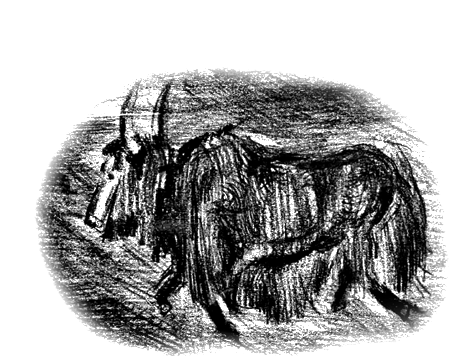
\includegraphics[height=3cm,right]{images/jak.png}\vspace*{-3.05cm}\\
  Jak suchy szloch w tę dżdżystą noc\\
  Pudowy kamień, pudowy kamień\\
  Ja na nim stanę, on na mnie stanie\\
  On na mnie stanie, spod niego wstanę\\
  Jak suchy szloch w tę dżdżystą noc\\
  Jak złota kula nad wodami\\
  Jak świt pod spuchniętymi powiekami\\
  \\
  Jak zorze miłe, śliczne polany\\
  Jak słońca pierś, jak garb swój nieść\\
  Jak do was, siostry mgławicowe, ten zawodzący śpiew\\
  \\
  Jak biec do końca, potem odpoczniesz\\
  Potem odpoczniesz, cudne manowce\\
  Cudne manowce, cudne, cudne manowce\\
\end{minipage}
\begin{minipage}[t]{0.25\textwidth}
  A E D A\\
  h D A (A$^4$)\\
  A E D A\\
  h D A (A$^4$)\\

  A E\\
  D A\\
  h D A (A$^4$)\\

  A E\\
  D A\\
  h D A (A$^4$)\\

  A E\\
  D A\\
  h D\\
  A A$^4$\\
  A E\\
  D A\\
  h D A (A$^4$)\\

  A E\\
  D A\\
  h D A (A$^4$)\\

  A E\\
  D A\\
  h D A (A$^4$)\\
\end{minipage}
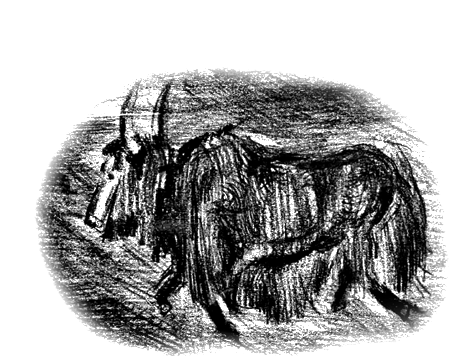
\includegraphics[width=0.5\textwidth,center]{images/jak.png}\\


\newpage
\section{Jaskółka uwięziona}\textcolor{lightgray}{\textit{Stan Borys}}\\~\\
\begin{minipage}[t]{0.8\textwidth}
  Jaskółka, czarny sztylet wydarty z piersi wiatru\\
  Nagła smutku kotwica z niewidzialnego jachtu\\
  Katedra ją złowiła w sklepienia sieć wysoką\\
  Jak śmierć - kamienna bryła, jak wyrok - naw prostokąt\\
  Jaskółka, błyskawica w kościele obumarłym\\
  Tnie, jak czarne nożyce lęk, który ją ogarnia\\

  \hspace*{5mm}Jaskółka, siostra burzy, żałoba fruwająca\\
  \hspace*{5mm}Ponad głowami ludzi, w których się troska błąka\\
  \hspace*{5mm}Jaskółka, znak podniebny, jak symbol nieuchwytna\\
  \hspace*{5mm}Zwabiona w chłód katedry, przestroga i modlitwa\\

  Nie przetnie białej ciszy pod chmurą ołowianą\\
  Lotu swego nie zniży nad łąki złotą plamą\\
  Przeraża mnie ta chwila, która jej wolność skradła\\
  Jaskółka, czarny brylant wrzucony tu przez diabła\\

  Na wieczne wirowanie, na bezszelestną mękę\\
  Na gniazda niezaznanie, na przeklinanie piękna\\
\end{minipage}
\begin{minipage}[t]{0.2\textwidth}
  h A e Fis\\h A e Fis\\h A e Fis\\h A e Fis\\h A e Fis\\h A e Fis\\

  h D fis, A (fis) h\\
  h D fis, A (fis) h\\
  h D fis, A (fis) h\\
  h D fis, A E\\

  h A e Fis\\h A e Fis\\h A e Fis\\h A e Fis\\

  h A e Fis\\h A e Fis\\
\end{minipage}

% TODO Jednego serca - Czesław Niemen
% \section{Jednego serca}\textcolor{lightgray}{\textit{Czesław Niemen}}\\~\\

\newpage
\section{Jesienne wino}\textcolor{lightgray}{\textit{Koczewski, Bogdański}}\\~\\
\begin{minipage}[t]{0.8\textwidth}
  Z brzękiem ostróg wjechałem do miasta\\
  Pod jesień było, czas złotych liści nastał\\
  W kieszeni worek srebra, czas do domu\\
  Wtem za plecami woła głos:\\
  \\
  \hspace*{5mm}Usiądź razem ze mną\\
  \hspace*{5mm}Spróbuj mego wina\\
  \hspace*{5mm}Z czereśni, wiśni, resztek lata\\
  \hspace*{5mm}Choć jesień się zaczyna\\
  \hspace*{5mm}Tyle tej jesieni\\
  \hspace*{5mm}Jeszcze jest przed nami\\
  \hspace*{5mm}Zdążysz wrócić do domu\\
  \hspace*{5mm}Nim noc zawita nad drogami\\
  ~\\
  \\
  Słońce stało w zenicie, bił południowy żar\\
  A w gardle kurz przebytych dróg\\
  Co tam, spocznę chwilę, przecież nie zaszkodzi\\
  Do przejścia niedaleką jeszcze drogę mam.\\
  A ona kusi:\\
  \\
  Zbudziłem się w czerwieniach zachodu\\
  Pod starą karczmą, co rynek zamyka\\
  Zabrała moje srebro, duszę i ostrogi\\
  Zostało pragnienie i tępy głowy ból.\\
  I pamięć jej słów:\\
\end{minipage}
\begin{minipage}[t]{0.2\textwidth}
  a G a G\\
  a G C C\\
  d C G a\\
  G F a G a G\\
  \\
  a C\\
  G C\\
  d C\\
  G F\\
  a C\\
  G C\\
  d C\\
  G F\\
  (a G a G)\\

  a G a G\\
  a G C C\\
  d C G a\\
  G F a G\\
  a G\\
  ~\\
  a G a G\\
  a G C C\\
  d C G a\\
  G F a G\\
  a G\\
\end{minipage}

\newpage
\section{Jesień idzie}\textcolor{lightgray}{\textit{Andrzej Waligórski}}\\~\\
\begin{minipage}[t]{0.6\textwidth}
  Raz staruszek, spacerując w lesie\\
  Ujrzał listek przywiędły i blady\\
  I pomyślał: Znowu idzie jesień\\
  Jesień idzie, nie ma na to rady\\

  \hspace*{4mm}I podreptał do chaty po dróżce\\
  \hspace*{4mm}I oznajmił, stanąwszy przed chatą\\
  \hspace*{4mm}Swojej żonie, tak samo staruszce\\
  \hspace*{4mm}Jesień idzie, nie ma rady na to\\
  \\
  Zaś staruszka zmartwiła się szczerze\\
  Zamachnęła rękami obiema\\
  Musisz zacząć chodzić w pulowerze\\
  Jesień idzie, rady na to nie ma\\

  \hspace*{4mm}Może zrobić się chłodno już jutro\\
  \hspace*{4mm}Lub pojutrze, a może za tydzień\\
  \hspace*{4mm}Trzeba będzie wyjąć z kufra futro\\
  \hspace*{4mm}Nie ma rady. Jesień, jesień idzie\\
  \\
  A był sierpień, pogoda prześliczna\\
  Wszystko w złocie trwało i w zieleni\\
  Prócz staruszków nikt chyba nie myślał\\
  O mającej nastąpić jesieni\\

  \hspace*{4mm}Ale cóż, oni żyli najdłużej\\
  \hspace*{4mm}Mieli swoje staruszkowie zasady\\
  \hspace*{4mm}I wiedzieli, że prędzej czy później\\
  \hspace*{4mm}Jesień przyjdzie. Nie ma na to rady\\
\end{minipage}
\begin{minipage}[t]{0.4\textwidth}
  e A$^7$ e A$^7$\\
  e A$^7$ H$^7$\\
  e A$^7$ e A$^7$\\
  C H$^7$ e A$^7$\\

  C D G e\\
  C D G e\\
  C D G e\\
  C H$^7$\\

  e A$^7$ e A$^7$\\
  e A$^7$ H$^7$\\
  e A$^7$ e A$^7$\\
  C H$^7$ e A$^7$\\

  C D G e\\
  C D G e\\
  C D G e\\
  C H$^7$\\

  e A$^7$ e A$^7$\\
  e A$^7$ H$^7$\\
  e A$^7$ e A$^7$\\
  C H$^7$ e A$^7$\\

  C D G e\\
  C D G e\\
  C D G e\\
  C H$^7$\\
\end{minipage}

\newpage
\section{Jest już za późno}\textcolor{lightgray}{\textit{SDM}}\\~\\
\begin{minipage}[t]{0.8\textwidth}
  Jeszcze zdążymy w dżungli ludzkości siebie odnaleźć\\
  Tęskność zawrotna przybliża nas\\
  Zbiegną się wreszcie tory sieroce naszych dwóch planet\\
  Cudnie spokrewnią się ciała nam\\
  \\
  \hspace*{5mm}Jest już za późno! (Nie jest za późno!)\\
  \hspace*{5mm}Jest już za późno! (Nie jest za późno!)\\
  \hspace*{5mm}Jest już za późno! (Nie jest za późno!)\\
  \\
  Jeszcze zdążymy tanio wynająć małą mansardę\\
  Z oknem na rzekę lub też na park\\
  Z łożem szerokim, piecem wysokim, ściennym zegarem\\
  Schodzić będziemy codziennie w świat\\
  \\
  Jeszcze zdążymy naszą miłością siebie zachwycić\\
  Siebie zachwycić i wszystko w krąg\\
  Wojna to będzie straszna, bo czas nas będzie chciał zniszczyć\\
  Lecz nam się uda zachwycić go\\

\end{minipage}
\begin{minipage}[t]{0.2\textwidth}
  G a G (C G)\\
  C G a D$^7$\\
  G a G (C G)\\
  C G a D$^7$\\

  h C\\
  h C\\
  h C a$^7$ D$^7$\\

  G a G (C G)\\
  C G a D$^7$\\
  G a G (C G)\\
  C G a D$^7$\\

  G a G (C G)\\
  C G a D$^7$\\
  G a G (C G)\\
  C G a D$^7$\\
\end{minipage}

\newpage
\section{Jeżeli kochać to nie indywidualnie}\textcolor{lightgray}{\textit{Kabaret starszych panów}}\\~\\
\begin{minipage}[t]{0.8\textwidth}
  \hspace*{4mm}Jeżeli kochać, jeżeli kochać, jeżeli kochać…\\
  \\
  Jeżeli kochać, to nie indywidualnie\\
  Jak się zakochać, to tylko we dwóch\\
  Czy platonicznie pragniesz jej, czy już sypialnie\\
  Niech w uczuciu wspiera wierny cię druh\\
  \\
  
\includegraphics[height=2cm, right]{images/jezeli_kochac.png}\vspace*{-20.5mm}\\
  Bo pojedynczo się z dziewczyną nie upora\\
  Ni dyplomata, ni mędrzec, ni wódz\\
  Więc ty drugiego sobie dobierz amatora\\
  I wespół w zespół, by żądz moc móc zmóc\\
  \\
  \hspace*{8mm}I wespół w zespół, wespół w zespół\\
  \hspace*{8mm}By żądz moc (!) móc zmóc\\
  \\
  Bo kiedy sam w zmysłów trwasz zawierusze\\
  To wszystek czas ci pochłonie i zdrowie\\
  Lecz gdy z oddanym kolegą, to tuszę\\
  Że tylko w połowie\\
  \\
  \hspace*{4mm}Wniosek?\\
  \hspace*{4mm}Jeżeli kochać, jeżeli kochać, jeżeli kochać…\\
  \\
  Jeżeli kochać, to dlaczego nie z kolegą?\\
  Dziewczynę wespół uwielbiać jest lżej\\
  Co niebezpieczne dla mężczyzny samotnego\\
  To z kolegą niebezpiecznym jest mniej\\
  \\
  Jeżeli kochać, to nie indywidualnie\\
  Jak się zakochać, to tylko we dwóch\\
  Czy platonicznie pragniesz jej, czy już sypialnie\\
  Niech w uczuciu wspiera wierny cię druh\\
  \\
  \hspace*{8mm}I wespół w zespół, wespół w zespół\\
  \hspace*{8mm}By żądz moc (!) móc zmóc\\
  \\
  A kiedy rzuci cię w szczęścia południe\\
  Kobieta z pięknym bezdusznym obliczem\\
  Dla samotnego to cios - aż zadudni\\
  Dla dwóch zaś, to prztyczek!\\

  \hspace*{4mm}Wniosek?\\
  \hspace*{4mm}Jeżeli kochać, jeżeli kochać, jeżeli kochać… \\
\end{minipage}
\begin{minipage}[t]{0.2\textwidth}
  f b G$^7$ C$^7$\\

  f b\\
  Dis Gis\\
  f G$^7$\\
  C$^7$ f\\

  f b\\
  Dis Gis\\
  f G$^7$\\
  C$^7$ f\\

  b f\\
  C$^7$ f\\

  f C$^7$\\
  C$^7$ f\\
  F$^7$ b\\
  G$^7$ C$^7$\\
  \\
  \\
  f b G$^7$ C$^7$\\

  f b\\
  Dis Gis\\
  f G$^7$\\
  C$^7$ f\\

  f b\\
  Dis Gis\\
  f G$^7$\\
  C$^7$ f\\

  b f\\
  C$^7$ f\\

  f b\\
  Dis Gis\\
  f G$^7$\\
  C$^7$ f\\
  \\
  \\
  f b G$^7$ C$^7$\\
\end{minipage}

\newpage
\section{Jeżożabki}\textcolor{lightgray}{\textit{Andrzej Rosiewicz}}\\~\\
\begin{minipage}[t]{0.8\textwidth}
  Na dużym, żółtym liściu w czasie dżdżu\\
  Siedziała żaba, czemu właśnie tu?\\
  Nie wiedział nikt i żaba chyba też\\
  Nie wiedziała. Siedząc żuła perz\\
  Kontemplowała deszcz, przeżuwając perz\\
  \\
  A nieopodal żaby kucnął jeż\\
  Dla towarzystwa żabie żuł coś też\\
  W jeżynach nagle żaba rzekła mu\\
  Ja cię żetem, mój żużu\\
  Naprawdę żetem, chcę cię teraz tu\\
  \\
  \hspace*{5mm}I w żabie wzięła go ramiona \\
  \hspace*{5mm}Kochanka-żaba, żaba-żona \\
  \hspace*{5mm}Spod żabich rzęs kapały żabie szczęścia łzy\\
  \hspace*{5mm}I tuli żabią twarz do jeża\\
  \hspace*{5mm}Jak hełm się tuli do żołnierza \\
  \hspace*{5mm}I tłumiąc łzy rzecze mu: only ty\\
  \\
  Czy w szczęściu nie przeszkodzi różna płeć?\\
  Zażenowany jeż chciał żabie rzec \\
  Nie zdążył, bo go żaba znów żetem\\
  I pieści dłoń, mami snem \\
  Pasjanse składa mu z samych żabich serc\\
  \\
  \hspace*{5mm}I szepcze mu: Mój mały książę\\
  \hspace*{5mm}Jeżeli kiedyś zajdę w ciążę \\
  \hspace*{5mm}Potomstwo mieć - to w życiu najpiękniejsza rzecz\\
  \hspace*{5mm}Urodzę tobie jeżożabki\\
  \hspace*{5mm}Tak trochę z ojca, trochę z matki\\
  \hspace*{5mm}Tak, jedno tę, drugie tę, pół na pół\\
  \\
  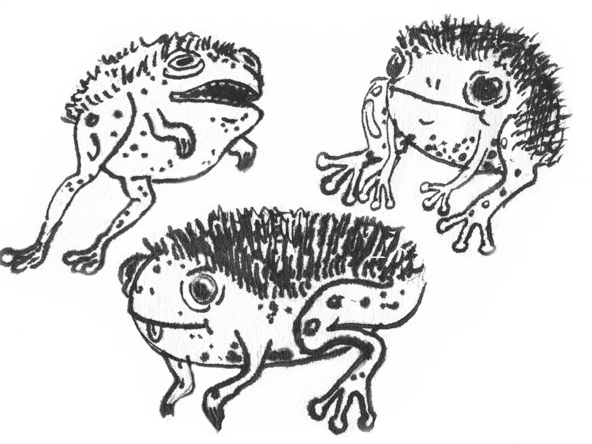
\includegraphics[height=3.4cm, right]{images/jezozabki.png}\vspace*{-3.4cm}\\
  Tak w życiu bywa, żabę kocha jeż\\
  Więc pomyśl ile szczęścia mógłbyś też\\
  Przy żabie znaleźć, gdybyś jeżem był\\
  Więc proszę cię z całych sił\\
  Mój drogi Jerzy, kochaj żabkę swą\\
  \\
  Byś i ty, mógł ronić szczęścia łzy\\
\end{minipage}
\begin{minipage}[t]{0.2\textwidth}
  e E$^7$\\
  a D$^7$\\
  G C\\
  G$^0$ a\\
  e H$^7$ e (H$^7$)\\

  e E$^7$\\
  a D$^7$\\
  G C\\
  G$^0$ a\\
  e H$^7$ e (E$^7$)\\

  a$^7$ D$^7$\\
  G C\\
  F$^7$ H$^7$ e (E$^7$)\\
  a$^7$ D$^7$\\
  G C\\
  F$^7$ H$^7$\\

  e E$^7$\\
  a D$^7$\\
  G C\\
  G$^0$ a\\
  e H$^7$ e (E$^7$)\\

  a$^7$ D$^7$\\
  G C\\
  F$^7$ H$^7$ e (E$^7$)\\
  a$^7$ D$^7$\\
  G C\\
  F$^7$ H$^7$\\

  e E$^7$\\
  a D$^7$\\
  G C\\
  G$^0$ a\\
  e H$^7$ e (E$^7$)\\

  F$^7$ e\\
\end{minipage}

\newpage
\section{Jolka, Jolka}\textcolor{lightgray}{\textit{Budka Suflera}}\\~\\
\begin{minipage}[t]{0.6\textwidth}
  Jolka, Jolka, pamiętasz lato ze snu\\
  Gdy pisałaś: tak mi źle!\\
  Urwij się choćby zaraz, coś ze mną zrób\\
  Nie zostawiaj tu samej, o nie\\

  Żebrząc wciąż o benzynę gnałem przez noc\\
  Silnik rzęził ostatkiem sił\\
  Aby być znowu w tobie, śmiać się i kląć\\
  Wszystko było tak proste w te dni\\

  Dziecko spało za ścianą czujne jak ptak\\
  Niechaj Bóg wyprostuje mu sny!\\
  Powiedziałaś, że nigdy, że nigdy aż tak\\
  Słodkie były jak krew twoje łzy\\

  \hspace*{6mm}Emigrowałem z objęć twych nad ranem\\
  \hspace*{6mm}Dzień mnie wyganiał, nocą znów wracałem\\
  \hspace*{6mm}Dane nam było słońca zaćmienie\\
  \hspace*{6mm}Następne będzie może za sto lat\\

  Plażą szły zakonnice, a słońce w dół\\
  Wciąż spadało nie mogąc spaść\\
  Mąż tam w świecie za funtem odkładał funt\\
  Na Toyotę przepiękną, aż strach\\

  Mąż twój wielbił porządek i pełne szkło\\
  Narzeczoną miał kiedyś jak sen\\
  Z autobusem Arabów zdradziła go\\
  Nigdy nie był już sobą, o nie\\
  \\
  \hspace*{6mm}Emigrowałem . . .\\
  \\
  W wielkiej żyliśmy wannie i rzadko tak\\
  Wypełzaliśmy na suchy ląd\\
  Czarodziejka gorzałka tańczyła w nas\\
  Meta była o dwa kroki stąd\\

  Nie wiem ciągle dlaczego zaczęło się tak\\
  Czemu zgasło też nie wie nikt\\
  Są wciąż różne koło mnie, nie budzę się sam\\
  Ale nic nie jest proste w te dni\\

\end{minipage}
\begin{minipage}[t]{0.4\textwidth}
  D A h\\
  D A h\\
  D A e h\\
  D A G\\

  D A h\\
  D A h\\
  D A e h\\
  D A G\\

  D A h\\
  D A h\\
  D A e h\\
  D A G\\

  \hspace*{3mm} e G D e G D\\
  \hspace*{3mm} e G D e G A\\
  \hspace*{3mm} e G D e G D\\
  \hspace*{3mm} e G D e G A\\

  D A h\\
  D A h\\
  D A e h\\
  D A G\\

  D A h\\
  D A h\\
  D A e h\\
  D A G\\
  ~\\~\\~\\
  D A h\\
  D A h\\
  D A e h\\
  D A G\\

  D A h\\
  D A h\\
  D A e h\\
  D A G\\
\end{minipage}

\newpage
\section{Justysia}\textcolor{lightgray}{\textit{Milano}}\\~\\
\begin{minipage}[t]{0.75\textwidth}
  Na Justysię czekałem przy studni\\
  Już myślałem, że przeminął wiek\\
  Nagle krok Justysi zadudnił\\
  Na mosteczku co wisiał w poprzek\\
  \\
  \hspace*{5mm}Sia la la, sia la la… a wieczór taki upojny\\
  \hspace*{5mm}Sia la la, sia la la… najważniejsze, że jestem przystojny\\
  \\
  Wreszcie jesteś, Justysiu ty ma\\
  Moja jedna, jedyna kochana\\
  Popatrz, księżyc na chmurkę się pcha\\
  A ty byś pewnie chciała na siano\\
  \\
  Na gałązce siadł sobie ptak\\
  Pewnie gałąź się pod nim nie złamie\\
  Bo by ptak wtedy upadł na wznak\\
  A ty byś pewnie chciała na sianie\\
  \\
  Ty byś chciała i ja też bym chciał\\
  Wrócić kiedyś do naszego zadupia\\
  Lecz nas los na poniewierkę skazał\\
  Bo tak chciał, czego ryczysz głupia\\
  \\
  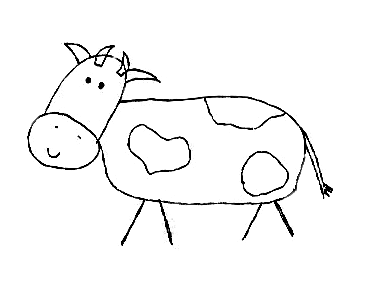
\includegraphics[height=4cm, angle=10, right]{images/justysia.png}\vspace*{-4.9cm}\\
  Raz zagroda spłonęła nam cała\\
  I chałupa też kryta dachówką\\
  Tyś mi jedna, Justysiu, została\\
  Holenderskiej rasy jałówko\\
  \\
\end{minipage}
\begin{minipage}[t]{0.25\textwidth}
  C\\
  C G\\
  G G$^7$\\
  G C (C$^7$)\\

  F C G (G$^7$) C C$^7$\\
  F C a G C (G C)\\
  \\
  \\
  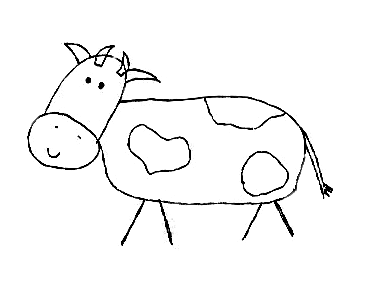
\includegraphics[width=\textwidth, angle=-15]{images/justysia.png}\\
\end{minipage}

\newpage
\section{Kakao}\textcolor{lightgray}{\textit{Mumio}}\\~\\
\begin{minipage}[t]{0.8\textwidth}
  Skończyła się już noc, żaluzje się rozjechały\\
  Na głowę naciągam koc, jest na mnie za mały\\
  Nogi wystają mi\\
  Jest mi zimno w nie\\
  (Prawdopodobnie) Nie kocham już ciebie\\

  Coś się musiało między nami\\
  Skomplikować\\
  Miłość\\
  Nie ma jej\\
  \\
  \hspace*{5mm}Jak to, jak to się stało\\
  \hspace*{5mm}Że mi wypiłaś moje kakao\\
  \hspace*{5mm}Przecież to mój kubeczek\\
  \hspace*{5mm}To mój kubeczek z wiewiórką jest\\

  ---\\

  \hspace*{5mm}Jak to, jak to się stało\\
  \hspace*{5mm}Że mi się tutaj przyjechać chciało\\
  \hspace*{5mm}Przecież tam był mój domek\\
  \hspace*{5mm}I ciepłe łóżko, i prysznic też\\
\end{minipage}
\begin{minipage}[t]{0.2\textwidth}
  (h$^{7-5}$) E a\\
  \\
  \\
  \chord{t}{n,p2,p3,p2,p3,n}{{\small h$^{7-5}$}}\\
\end{minipage}
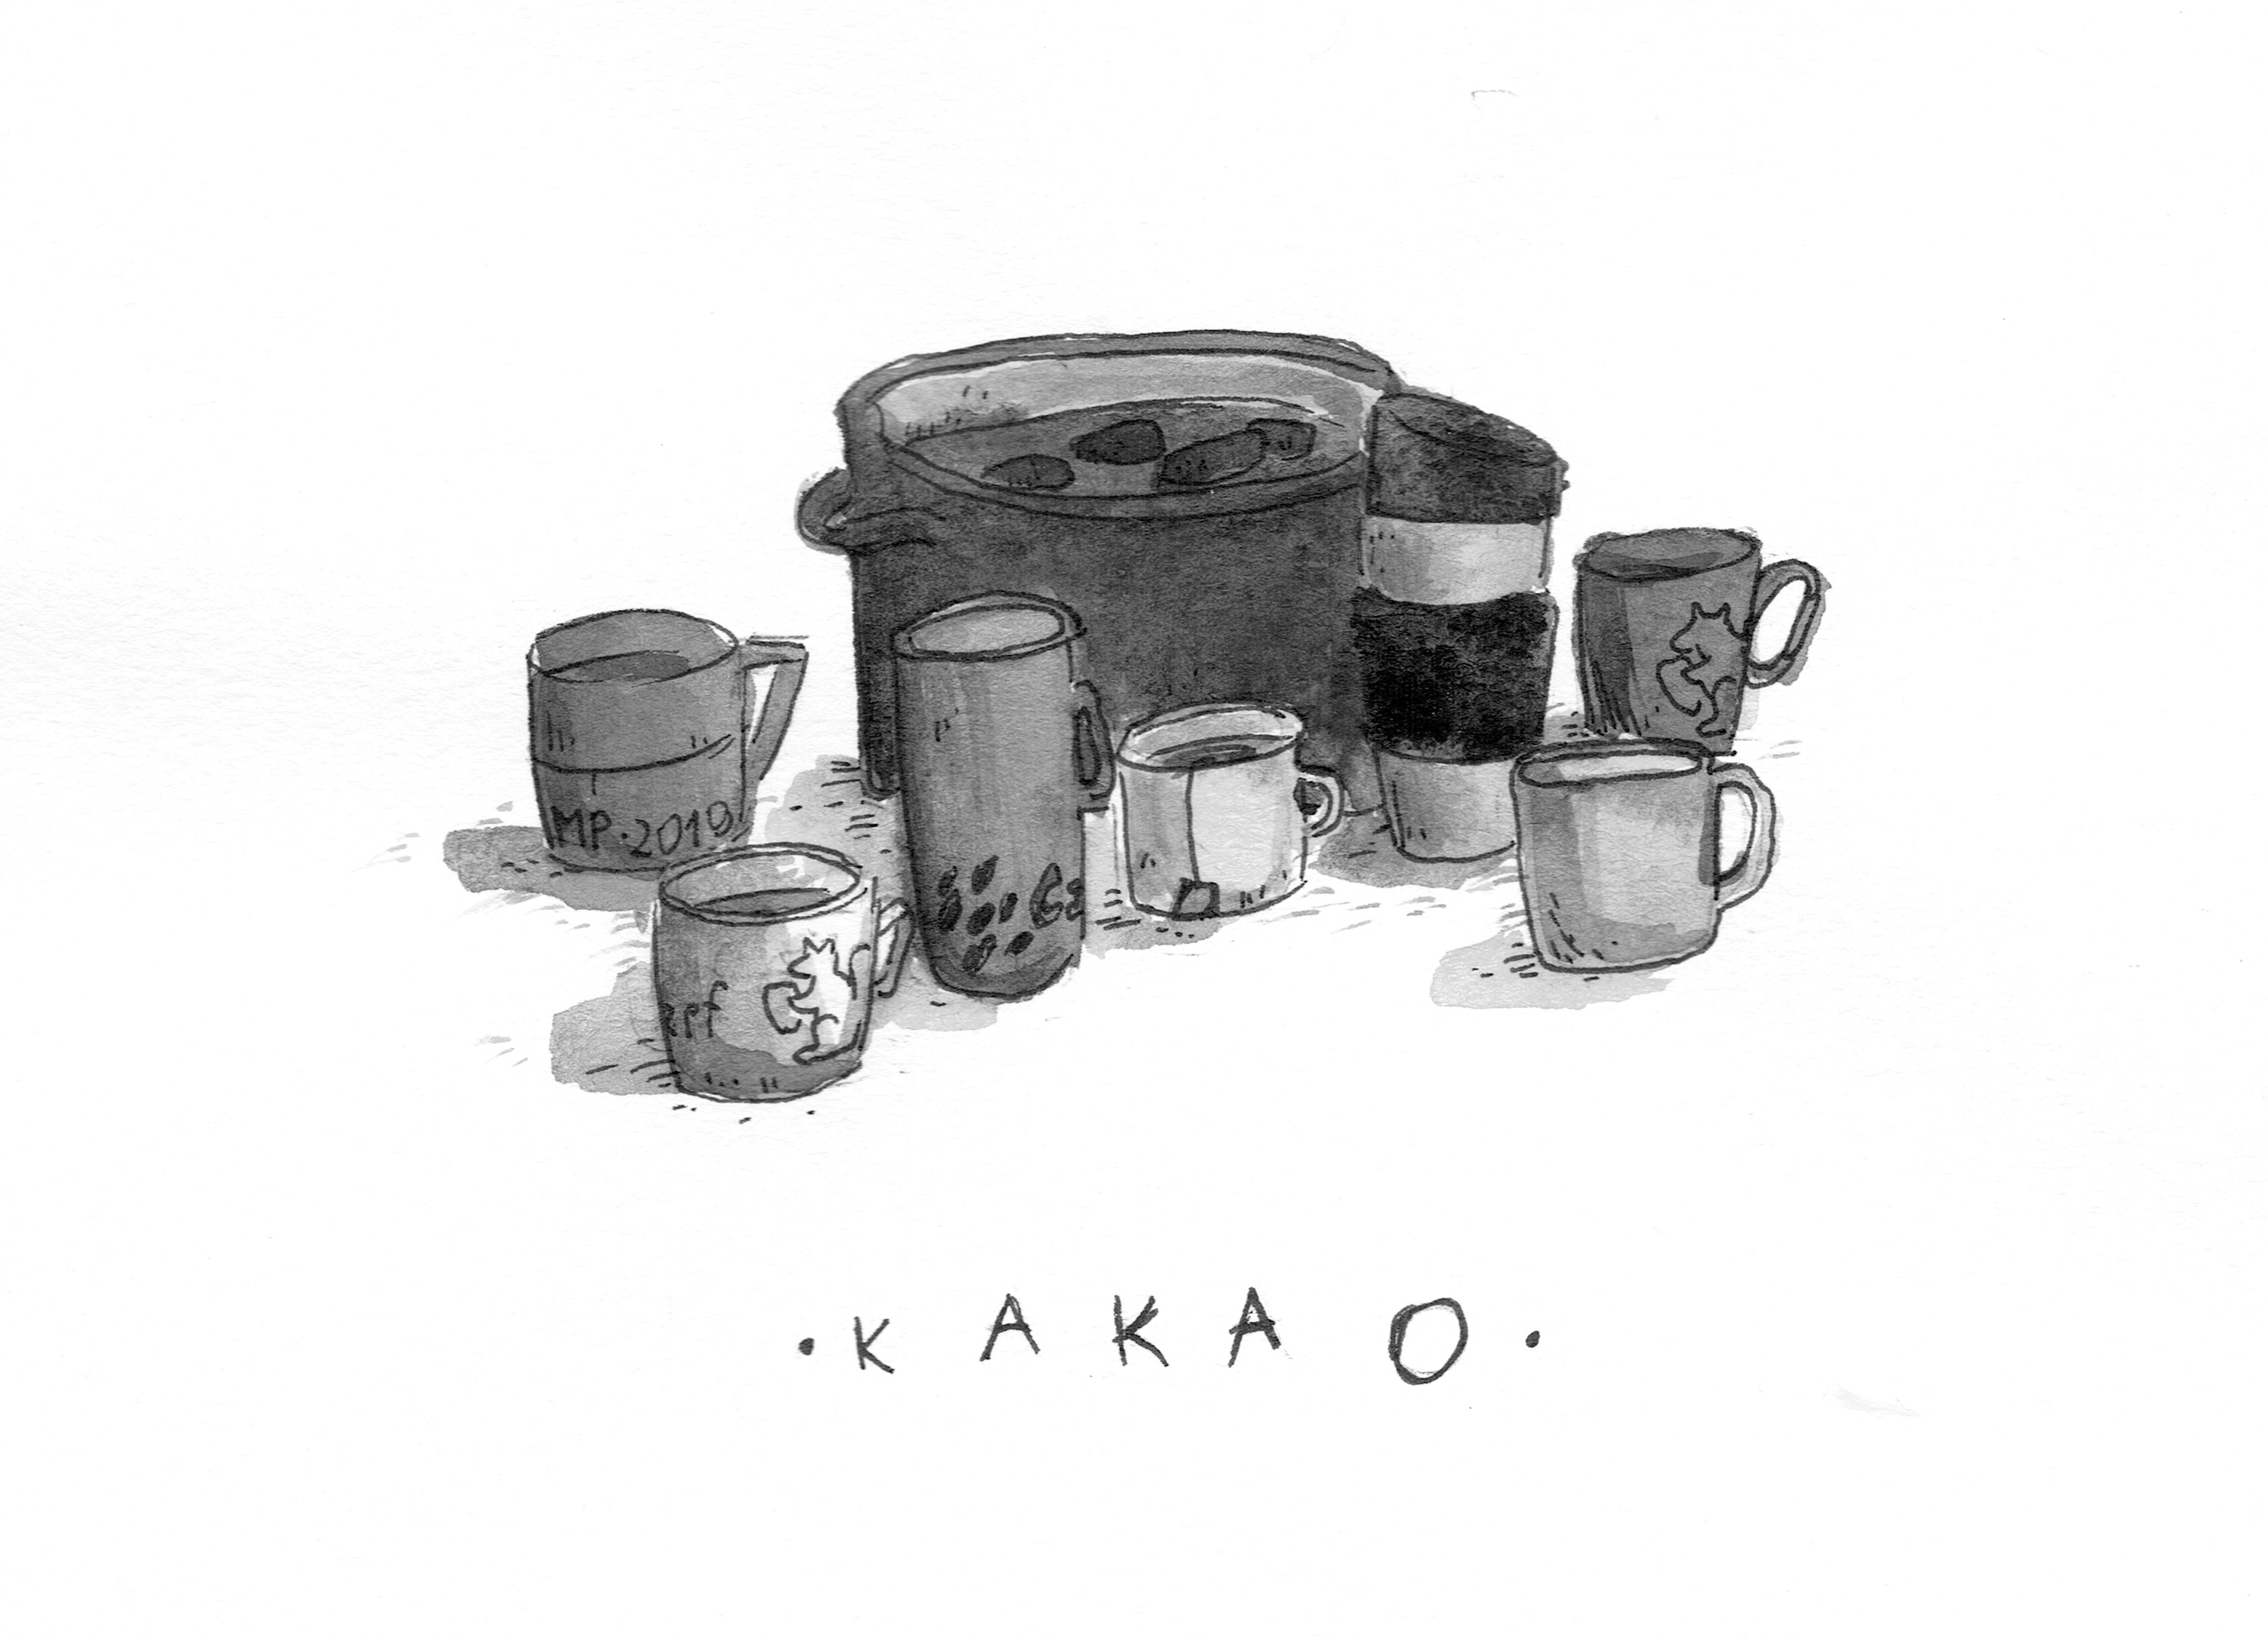
\includegraphics[width=0.85\textwidth, center]{images/kakao.png}\\

\newpage
\section{Kantyczka z lotu ptaka}\textcolor{lightgray}{\textit{Kaczmarski, Gintrowski, Łapiński}}\\~\\
\begin{minipage}[t]{0.82\textwidth}
  Patrz mój dobrotliwy Boże na swój ulubiony ludek,\\
  Jak wychodzi rano w zboże zginać harde karki z trudem.\\
  Patrz, jak schyla się nad pracą, jak pokornie klęski znosi\\
  I nie pyta - Po co? Za co? Czasem o coś Cię poprosi:\\
  \\
  \hspace*{3mm}Ujmij trochę łaski nieba! Daj spokoju w zamian, chleba!\\
  \hspace*{3mm}Innym udziel swej miłości! Nam - sprawiedliwości!\\
  \\
  Smuć się, Chryste Panie w chmurze widząc, jak się naród bawi,\\
  Znowu chciałby być przedmurzem i w pogańskiej krwi się pławić.\\
  Dymią kuźnie i warsztaty, lecz nie pracą a - skargami,\\
  Że nie taka, jak przed laty łaska Twoja nad hufcami:\\
  \\
  \hspace*{3mm}Siły grożą Ci nieczyste daj nam wsławić się, o Chryste!\\
  \hspace*{3mm}Kalwin, Litwin nam ubliża! Dźwigniem ciężar Krzyża!\\
  \\
  Załam ręce Matko Boska, upadają obyczaje,\\
  Nie pomogła modłom chłosta - młodzież w szranki ciała staje.\\
  W nędzy gzi się krew gorąca bez sumienia, bez oddechu,\\
  Po czym z własnych trzewi strząsa niedojrzały owoc grzechu.\\
  \\
  \hspace*{3mm}- Co zbawienie nam, czy piekło! Byle życie nie uciekło!\\
  \hspace*{3mm}Jeszcze będzie czas umierać! Żyjmy tu i teraz!\\
  \\
  Grzmijcie gniewem Wszyscy Święci, handel lud zalewa boży\\
  Obce kupce i klienci w złote wabią go obroże.\\
  Liczy chciwy Żyd i Niemiec dziś po ile polska czystość;\\
  Kupi dusze, kupi ziemie i zostawi pośmiewisko...\\
  \\
  \hspace*{3mm}Co nam hańba, gdy talary, Mają lepszy kurs od wiary!\\
  \hspace*{3mm}Wymienimy na walutę, Honor i pokutę!\\
  \\
  Jeden naród, tyle kwestii! Wszystkich naraz nie wysłuchasz!\\
  Zadumali się Niebiescy w imię Ojca, Syna, Ducha...\\
  Co nam hańba, gdy talary...\\
\end{minipage}
\begin{minipage}[t]{0.25\textwidth}
  a C\\
  G E$^7$\\
  a C\\
  G E$^7$\\

  a E$^7$ a, C G\\
  E$^7$ a, F aE$^7$\\

  a C\\
  G E$^7$\\
  a C\\
  G E$^7$\\

  a E$^7$ a, C G\\
  E$^7$ a, F aE$^7$\\

  a C\\
  G E$^7$\\
  a C\\
  G E$^7$\\

  a E$^7$ a, C G\\
  E$^7$ a, F aE$^7$\\

  a C\\
  G E$^7$\\
  a C\\
  G E$^7$\\

  a E$^7$ a, C G\\
  E$^7$ a, F aE$^7$\\

  a C\\
  G E$^7$\\
\end{minipage}

\newpage
\section{Każdego dnia}\textcolor{lightgray}{\textit{Ola Kwaśniewska, VII 2015}}\\~\\
\begin{minipage}[t]{0.8\textwidth}
  \hspace*{5mm}Każdego dnia nad horyzontem słońce wznosi dłoń		\\
  \hspace*{5mm}By ciepłym jej dotknięciem ziemię w posiadanie wziąć	\\
  \hspace*{5mm}Każdego dnia przez szum podniebnych sosen wiedzie szlak\\
  \hspace*{5mm}I pragnę, by już zawsze było tak\\
  \\
  Wszystko w naturze położenie swoje zmienia\\
  Bezruchu znieść nie może nasza stara Ziemia\\
  I w ludzkich snach też pojawiają się marzenia\\
  O choć chwilowej zmianie punktu odniesienia\\
  Więc wyruszamy, porzucając wytarty ślad\\
  Rysując nowe ścieżki w zieleni łąk\\
  Łagodny wiatr nad oceanem rozgrzanych traw\\
  Unosi myśli bardzo daleko stąd\\
  \\
  Już cały czas chciałabym tak wędrować razem z wami\\
  Czuć niebo ponad sobą i kamienie pod stopami\\
  Słuchać chóru waszych głosów wieczorami\\
  Takich wspomnień nie wymieniłabym na nic\\
  Lecz trzeba nam w nurt codzienności włączyć się znów\\
  Ze stóp zmęczonych zetrzeć pył wielu dróg\\
  Pod powiekami zostaną kształty wysokich chmur\\
  A w głowie myśli, którym nie potrzeba słów\\
\end{minipage}
\begin{minipage}[t]{0.2\textwidth}
  d g\\
  C d\\
\end{minipage}

\newpage
\section{Kebab w cienkim cieście}\textcolor{lightgray}{\textit{Zacier}}\\~\\
\begin{minipage}[t]{0.8\textwidth}
  Wyszedłem dzisiaj z roboty, gdyż nie miałem co robić\\
  W robocie (hey yeah)\\
  Poszedłem do Turka na rogu i mówię mu: daj mi proszę\\
  Kebab w cienkim cieście (oh yeah)\\
  A on mi na to, że niestety zabrakło baraniny (oh no)\\
  \\
  \hspace*{5mm}Kebab w cienkim cieście\\
  \hspace*{5mm}Po nocach mi się śni, po nocach mi się śni\\
  \hspace*{5mm}Kebab w cienkim cieście\\
  \hspace*{5mm}O dajcież dzisiaj mi, och dajcież mi, dajcież mi\\

  \hspace*{5mm}Kebab w cienkim cieście\\
  \hspace*{5mm}Po nocach mi się śni, tib tibi dibidi\\
  \hspace*{5mm}Kebab w cienkim cieście\\
  \hspace*{5mm}Dajcież mi\\
  \\
  Odszedłem niepocieszony i do nocy włóczyłem się\\
  Po moim mieście (oh yeah)\\
  Lecz na zawsze zapadną w mej pamięci te słowa, jakże okrutne\\
  I złowieszcze (hey yeah)\\
  Bo to dzisiaj, właśnie dzisiaj zabrakło baraniny (oh no)\\
  \\
  Już nigdy nie pójdę na kebab i do śmierci będę żywił się\\
  Jajecznicą (oh no)\\
  Lecz czasem serce me zadrży i zaskowyczę, niczym hiena\\
  Nad Pilicą (oh yeah)\\
  Bo to dzisiaj, właśnie dzisiaj zabrakło baraniny (oh no)\\
\end{minipage}
\begin{minipage}[t]{0.2\textwidth}
  cis A fis\\
  cis A H A\\
  cis A fis\\
  cis A H A\\
  D E fis (E fis)\\

  fis\\
  D\\
  E cis\\
  fis (E fis)\\

  fis\\
  D\\
  E cis\\
  fis (E fis)\\

  cis A fis\\
  cis A H A\\
  cis A fis\\
  cis A H A\\
  D E fis (E fis)\\

  cis A fis\\
  cis A H A\\
  cis A fis\\
  cis A H A\\
  D E fis (E fis)\\
\end{minipage}

\newpage
\section{Kiler}\textcolor{lightgray}{\textit{Elektryczne gitary}}\\~\\
\begin{minipage}[t]{0.7\textwidth}
  To, co się dzieje, naprawdę nie istnieje\\
  Więc nie warto mieć niczego, tylko karmić zmysły\\
  Będzie, co ma być, już wiem, że stąd nie zwieję\\
  Poczekam i popatrzę, nie cofnę kijem Wisły\\
  \\
  \hspace*{6mm}Już tylko Kiler, o sobie tylko tyle\\
  \hspace*{6mm}Wiem co za ile, nie muszę dbać o bilet\\
  \hspace*{6mm}Mam wszystko w tyle, są czasem takie chwile\\
  \hspace*{6mm}Że się nie mylę, choć wcale nie wiem ile\\
  \\
  Nie kiwnąłem nawet palcem\\
  By się znaleźć w takiej walce\\
  Teraz w pace swe ostatnie resztki imidżu tracę\\
  \hspace*{3mm}(tuturuturututu...)\\
  Co się ze mną dzieje, naprawdę nie istnieję\\
  Więc nie warto tak się bronić, tylko lecieć z wiatrem\\
  Poczekam, popatrzę, zrozumiem więcej\\
  I wtedy wreszcie sam też włączę się do akcji\\
  \\
  \hspace*{6mm}Już tylko Kiler. . .\\
  \hspace*{3mm}(tuturuturututu...)\\
  Już tylko Kiler, podniosłem bilę\\
  Wracam za chwilę, nie dbam o bagaż, nie dbam o bilet\\
  Już tylko Kiler, nie, nie, ooo\\
  Mam wszystko w tyle, wiem co za ile, może się mylę\\
  To chyba thriller, ajajajajajajajaj\\

\end{minipage}
\begin{minipage}[t]{0.3\textwidth}
  D\\
  e A D\\
  D\\
  e A D\\

  h fis e A\\
  h fis e A\\
  h fis e A\\
  h fis e A\\

  G\\
  D A\\
  G D A\\
  (G D A G D A)\\
  D\\
  e A D\\
  D\\
  e A D\\

  ~\\
  (G D A G D A)\\
  h fis\\
  e A\\
  h fis e A\\
  h fis e A\\
  h fis e A\\
\end{minipage}

\newpage
\section{Killing me softly}\textcolor{lightgray}{\textit{Roberta Flack}}\\~\\
\begin{minipage}[t]{0.75\textwidth}
  \hspace*{5mm}Strumming my pain with his fingers \\
  \hspace*{5mm}Singing my life with his words\\
  \hspace*{5mm}Killing me softly with his song, \\
  \hspace*{5mm}Killing me softly with his song \\
  \hspace*{5mm}Telling my whole life with his words \\
  \hspace*{5mm}Killing me softly with his song\\
  \\
  I heard he sang a good song I heard he had a style\\
  And so I came to see him to listen for a while\\
  And there he was this young boy, a stranger to my eyes\\
  \\
  I felt all flushed with fever embarrassed by the crowd\\
  I felt he found my letters and read each one out loud\\
  I prayed that he would finish, but he just kept right on\\
  \\
  He sang as if he knew me in all my dark despair \\
  And then he looked right through me As if I wasn't there \\
  And he just kept on singing singing clear and strong \\

\end{minipage}
\begin{minipage}[t]{0.25\textwidth}
  e a\\
  D$^7$ G\\
  e A\\
  D C\\
  G C\\
  F E$^4$E\\

  a$^7$ D G C\\
  a$^7$ D e\\
  a$^7$ D$^7$ G H$^7$\\

  a$^7$ D G C\\
  a$^7$ D e\\
  a$^7$ D$^7$ G H$^7$\\

  a$^7$ D G C\\
  a$^7$ D e\\
  a$^7$ D$^7$ G H$^7$\\
\end{minipage}

% \newpage
\section{Kim właściwie była ta piękna pani}\textcolor{lightgray}{\textit{SDM}}\\~\\
\begin{minipage}[t]{0.8\textwidth}
  Nikt nie zna ścieżek gwiazd, wybrańcem - kto wśród nas\\
  Zapukał ktoś - to do mnie gość?\\
  Włóczyłem się jak cień, czekałem na ten dzień\\
  Już stoisz w drzwiach jak dziwny ptak\\
  \hspace*{5mm} Więc bardzo proszę, wejdź, tu siadaj, rozgość się\\
  \hspace*{5mm} I zdradź mi, kim tyś jest, Madame?\\
  \hspace*{5mm} Albo nie zdradzaj mi, lepiej nie mówmy nic\\
  \hspace*{5mm} Lepiej nie mówmy nic\\
  \\
  Nieśmiało sunie brzask, zatrzymać chciałbym czas\\
  Inaczej jest - czas musi biec\\
  Gdzieś w dali zapiał kur, niemodny wdziewasz strój\\
  Już stoisz w drzwiach jak dziwny ptak\\
  \hspace*{5mm}Więc jednak musisz pójść, posyłasz mi przez próg\\
  \hspace*{5mm}Ulotny uśmiech twój, Madame\\
  \hspace*{5mm}Lecz będę czekać, przyjdź! Gdy tylko zechcesz, przyjdź\\
  \hspace*{5mm}Będziemy razem żyć\\

\end{minipage}
\begin{minipage}[t]{0.2\textwidth}
  a G e a\\
  d C G \\
  a G e a\\
  d C G \\
  F G e a\\
  F G \\
  e a G \\
  F C \\

  a G e a\\
  d C G \\
  a G e a\\
  d C G \\
  F G e a\\
  F G \\
  e a G \\
  F C \\
\end{minipage}

% \section{Klosz} % TODO


\newpage
\section{Knockin' on the heaven's door}\textcolor{lightgray}{\textit{Bob Dylan}}\\~\\
\begin{minipage}[t]{0.7\textwidth}
  Mama, take this badge from me				\\
  I can't use it anymore		\\
  It's gettin' dark, too dark to see\\
  Feels like I'm knockin' on heaven's door\\
  \\
  \hspace*{5mm}Knock, knock, knockin' on heaven's door ~~~~~~$\times$4\\
  \\
  Mama, put my guns in the ground\\
  I can't shoot them anymore\\
  That long black cloud is comin' down\\
  I feel like I'm knockin' on heaven's door\\
  \\
  Baby stay right here with me\\
  'Cause I can't see you anymore\\
  This ain't the way it's supposed to be\\
  I feel I'm knocking on heaven's door\\
  \\
  Son, won't you remember me?\\
  I can't be with you anymore\\
  A lawman's life is never free\\
  I feel I'm knocking on heaven's door\\
\end{minipage}
\begin{minipage}[t]{0.3\textwidth}
  G D a$^7$\\
  G D C\\
  G D a$^7$\\
  G D C\\

  G D a$^7$ / G D C $\times$2\\

  G D a$^7$\\
  G D C\\
  G D a$^7$\\
  G D C\\

  G D a$^7$\\
  G D C\\
  G D a$^7$\\
  G D C\\

  G D a$^7$\\
  G D C\\
  G D a$^7$\\
  G D C\\

\end{minipage}

\newpage
\section{Kochałem cię dziś rano}\textcolor{lightgray}{\textit{Paweł Orkisz}}\\~\\
\begin{minipage}[t]{0.8\textwidth}
  Kochałem cię dziś rano, ust naszych ciepła słodycz\\
  Jak senna złota burza nade mną Twoje włosy\\
  Przed nami na tym świecie już inni się kochali\\
  I w mieście albo w lesie też tak się uśmiechali\\
  A teraz trzeba zacząć rozłączać się po trochu\\
  \\
  \hspace*{5mm}Twe oczy posmutniały\\
  \hspace*{5mm}Maleńka, nie wolno się żegnać\\
  \hspace*{5mm}W ten sposób\\
  \\
  Na pewno cię nie zdradzę, odprowadź mnie do rogu\\
  Ty wiesz, że nasze kroki zrymują się ze sobą\\
  Twa miłość pójdzie ze mną, a moja tu zostanie\\
  I będą się zmieniały jak brzeg i morskie fale\\
  Czy miłość to kajdany? Nie mówmy lepiej o tym\\
\end{minipage}
\begin{minipage}[t]{0.2\textwidth}
  A\\
  fis\\
  D\\
  A\\
  fis\\

  D\\
  E\\
  A E\\

  A\\
  fis\\
  D\\
  A\\
  fis\\
\end{minipage}

% \newpage
\section{Kolorowe jarmarki}\textcolor{lightgray}{\textit{Janusz Laskowski
  }}\\~\\
\begin{minipage}[b]{0.82\textwidth}
  Kiedy patrzę hen za siebie, w tamte lata co minęły\\
  Czasem myślę, co przegrałam, ile diabli wzięli\\
  Co straciłam z własnej woli, a co przeciw sobie\\
  Co wyliczę, to wyliczę, ale zawsze wtedy powiem\\
  Że najbardziej mi żal\\
  \\
  \hspace*{4mm}Kolorowych jarmarków, blaszanych zegarków\\
  \hspace*{4mm}Pierzastych kogucików, baloników na druciku\\
  \hspace*{4mm}Motyli drewnianych, koników bujanych\\
  \hspace*{4mm}Cukrowej waty i z piernika chaty\\
  \\
  Gdy w dzieciństwa wracam strony, dobre chwile przypominam\\
  Mego miasta słyszę strony, czy ktoś czas zatrzymał\\
  I gdy pytam cicho siebie: Czego żal dziś tobie\\
  Co wyliczę to wyliczę, ale zawsze wtedy powiem\\
  Że najbardziej mi żal\\
\end{minipage}
\begin{minipage}[b]{0.18\textwidth}
  a d \\
  G   C E$^7$\\
  d G C a\\
  E   E$^7$\\
  a\\
  \\
  d G C a\\
  d E$^7$ a A$^7$\\
  d G C a\\
  d E$^7$ a\\

  a d \\
  G C E$^7$\\
  d G C a\\
  E   E$^7$\\
  a \\
\end{minipage}

\newpage
\section{Kolorowy wiatr}\textcolor{lightgray}{\textit{Edyta Górniak}}\vspace*{1.5mm}\\
\begin{minipage}[t]{0.8\textwidth}
  \hspace*{3mm}Masz mnie za głupią dzikuskę\\
  \hspace*{3mm}Lecz choć cały świat zwiedziłeś\\
  \hspace*{3mm}Zjeździłeś wzdłuż i wszerz\\
  \hspace*{3mm}I mądry jesteś tak, że aż słów podziwu brak\\
  \hspace*{3mm}Dlaczego, powiedz mi, tak mało wiesz?\\
  \hspace*{3mm}Mało wiesz\\
  \\
  Na lądzie, gdy rozglądasz się lądując\\
  Chcesz wszystko mieć na własność, nawet głaz\\
  A ja wiem, że ten głaz ma także duszę\\
  Imię ma i zaklęty w sobie czas\vspace*{1.5mm}\\
  Ty myślisz, że są ludźmi tylko ludzie\\
  Których ludźmi nazywać chce twój świat\\
  Lecz jeśli pójdziesz tropem moich braci \\
  Dowiesz się największych prawd, najświętszych prawd \\
  \\
  \hspace*{5mm}Czy wiesz, czemu wilk tak wyje w księżycową noc?\\
  \hspace*{5mm}I czemu ryś tak zęby szczerzy rad?\\
  \hspace*{5mm}Czy powtórzysz tę melodię, co z gór płynie?\\
  \hspace*{5mm}Barwy, które kolorowy niesie wiatr\\
  \hspace*{5mm}Barwy, które kolorowy niesie wiatr\\
  \\
  Pobiegnij za mną leśnych duktów szlakiem\\
  Spróbujmy jagód w pełne słońca dni\\
  Zanurzmy się w tych skarbach niezmierzonych\\
  I choć raz o ich cenach nie mów nic\vspace*{1.5mm}\\
  Ulewa jest mą siostrą, strumień bratem\\
  A każde z żywych stworzeń to mój druh\\
  Jesteśmy połączonym z sobą światem\\
  A natura ten krąg życia wprawia w ruch\\
  \\
  \hspace*{8mm}Do chmur każde drzewo się pnie \\
  \hspace*{8mm}Skąd to wiedzieć masz, skoro ścinasz je?\vspace*{1.5mm}\\
  \hspace*{5mm}To nie tobie ptak się zwierza w księżycową noc\\
  \hspace*{5mm}Lecz ludziom wszelkich ras i wszelkich wiar\\
  \hspace*{5mm}Więc zanućmy tę melodię, co z gór płynie\\
  \hspace*{5mm}Barwy, które kolorowy niesie wiatr\vspace*{1.5mm}\\
  \hspace*{8mm}Możesz zdobyć świat\\
  \hspace*{8mm}Lecz to będzie tylko świat\\
  \hspace*{8mm}Tylko świat \\
  \hspace*{8mm}Nie barwy, które niesie wiatr \\

\end{minipage}
\begin{minipage}[t]{0.2\textwidth}
  c B\\
  c\\
  g\\
  c g c B\\
  c B G\\
  g C\\
  \\
  C a\\
  C e\\
  F e d\\
  d e a\vspace*{1.5mm}\\
  C a\\
  C e\\
  F e d\\
  d G C\\

  a e F\\
  a e\\
  F G C\\
  d F G\\
  d F C\\

  C a\\
  C e\\
  F e d\\
  d e a\vspace*{1.5mm}\\
  C a\\
  C e\\
  F e d\\
  d G C\\

  F e a\\
  d G\vspace*{1.5mm}\\
  a e F\\
  a e\\
  F G C\\
  d F G\vspace*{1.5mm}\\
  d G\\
  e F\\
  a\\
  e F G C\\
\end{minipage}

\newpage
\section{Kołysanka dla nieznajomej}\textcolor{lightgray}{\textit{Perfect}}\\~\\
\begin{minipage}[t]{0.7\textwidth}
  Gdy nie bawi cię już\\
  Świat zabawek mechanicznych\\
  Kiedy dręczy cię ból\\
  Niefizyczny\\
  Zamiast słuchać bzdur\\
  Głupich telefonicznych wróżek zza siedmiu mórz\\
  Spytaj siebie czego pragniesz\\
  Dlaczego kłamiesz, że miałaś wszystko\\

  Gdy udając że śpisz\\
  W głowie tropisz bajki z gazet\\
  Kiedy nie chcesz już śnić\\
  Cudzych marzeń\\
  Bosa do mnie przyjdź\\
  I od progu bezwstydnie powiedz mi czego chcesz\\
  Słuchaj jak dwa serca biją\\
  Co ludzie myślą to nieistotne\\

  \hspace*{5mm}Kochaj mnie   \hspace*{8mm} $\times$2\\
  \hspace*{5mm}Kochaj mnie nieprzytomnie\\
  \hspace*{5mm}Jak zapalniczka płomień\\
  \hspace*{5mm}Jak sucha studnia wodę\\
  \hspace*{5mm}Kochaj mnie namiętnie tak\\
  \hspace*{5mm}Jakby świat się skończyć miał\\

  Swoje miejsce znajdź\\
  I nie pytaj czy taki układ ma jakiś sens\\
  Słuchaj co twe ciało mówi\\
  W miłosnej studni już nie utoniesz\\

  \hspace*{5mm}Kochaj mnie  \hspace*{8mm} $\times$2\\
  \hspace*{5mm}Kochaj mnie nieprzytomnie\\
  \hspace*{5mm}Jak zapalniczka płomień\\
  \hspace*{5mm}Jak sucha studnia wodę\\

  \hspace*{5mm}Kochaj mnie  \hspace*{8mm} $\times$2\\
  \hspace*{5mm}Kochaj mnie nieprzytomnie\\
  \hspace*{5mm}Jak księżyc w oknie śmiej się i płacz\\
  \hspace*{5mm}Na linie nad przepaścią tańcz\\
  \hspace*{5mm}Aż w jedną krótką chwilę\\
  \hspace*{5mm}Pojmiesz po co żyjesz\\
\end{minipage}
\begin{minipage}[t]{0.3\textwidth}
  C a\\
  F (G)\\
  C a\\
  F (G)\\
  C\\
  a e F\\
  G a\\
  F G\\
  \\
  C a\\
  F (G)\\
  C a\\
  F (G)\\
  C\\
  a e F\\
  G a\\
  F G\\
  \\
  C G$^7$ a$^7$ G  \hspace*{5mm}$\times$2\\
  C G$^7$ a$^7$\\
  e\\
  F G F\\
  F G a F\\
  G C\\

  C\\
  a e F\\
  G a\\
  F G\\

  C G$^7$ a$^7$ G  \hspace*{5mm}$\times$2\\
  C G$^7$ a$^7$\\
  e\\
  F G F\\

  C G$^7$ a$^7$ G  \hspace*{5mm}$\times$2\\
  C G$^7$ a$^7$\\
  e\\
  F G F\\
  G a\\
  F G\\

\end{minipage}

\newpage
\section{Krajka}\textcolor{lightgray}{\textit{WBH}}\vspace*{2mm}\\
\begin{minipage}[t]{0.87\textwidth}
  Chorałem dzwonków dzień rozkwita, jeszcze od rosy rzęsy mokre \\
  We mgle turkoce pierwsza bryka, słońce wyrusza na włóczęgę\\
  Drogą pylistą, drogą polną, jak kolorowa panny krajka\\
  Słońce się wznosi nad stodołą, będzie tańczyć walca\\

  \hspace*{5mm}A ja mam swą gitarę, spodnie wytarte i buty stare\\
  \hspace*{5mm}Wiatry niosą mnie na skrzydłach\\
  \hspace*{5mm}A ja mam swą gitarę, spodnie wytarte i buty stare\\
  \hspace*{5mm}Wiatry niosą mnie nie wiadomo gdzie\\
  \vspace*{5mm}\\
  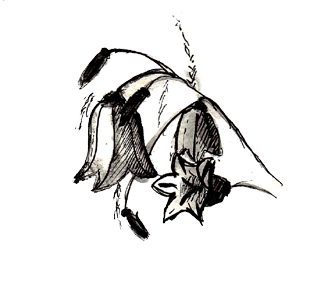
\includegraphics[height=2cm, right]{images/krajka.png}\vspace*{-2.55cm}\\
  Zmoknięte świerszcze stroją skrzypce, żuraw się wsparł o cembrowinę\\
  Wiele nanosi wody jeszcze, wielu się ludzi z niej napije\\
  Drogą pylistą, drogą polną, jak kolorowa panny krajka\\
  Słońce się wznosi nad stodołą, będzie tańczyć walca\\
\end{minipage}
\begin{minipage}[t]{0.13\textwidth}
  a d E a F G\\
  C d E E$^7$\\
  a d E a F G\\
  C d E E$^7$\\

  F G C a\\
  d E a A$^7$\\
  F G C a\\
  d E a E a\\

  a d E a F G\\
  C d E E$^7$\\
  a d E a F G\\
  C d E E$^7$\\
\end{minipage}

% \newpage
\section{Kto powie mi jak}\textcolor{lightgray}{\textit{Kwiat Jabłoni}}\vspace*{2mm}\\
\begin{minipage}[t]{0.8\textwidth}
  Stoję gdzieś pod niebem, pod nogami piach\\
  Mam podobno iść przed siebie\\
  Chociaż nie wiem jak, oj nie wiem\\
  Robię pierwszy krok, muszę więc gdzieś dojść\\
  Góra wielka, droga kręta\\
  Trudno czasem iść, nie stękać\\
  Chcę od razu wiedzieć na czym stoi świat\\
  Jak poznawać siebie lepiej\\
  Jak nie potknąć się o ciebie\\
  Idąc byle jak\vspace*{1.9mm}

  \hspace*{5mm}Więc kto powie mi jak radzić sobie mam \\
  \hspace*{5mm}Taki wielki świat nade mną mam \\
  \hspace*{5mm}Ileś tam lat, lecz to niewiele da\\
  \hspace*{5mm}Doświadczenia (ciągle) brak\\
  \\
  Będziesz w pocie czoła walczyć o swój świat\\
  Będziesz wodą żyć i chlebem\\
  Myśleć będziesz nad swym celem\\
  Tak podobno mówił On człowiekowi co\\
  Zbłądził jedząc owoc wiedzy\\
  Bo chciał wiedzieć co miał wiedzieć\\
  Tak już w życiu bywa od zarania lat\\
  Że ktoś winny musi być\\
  Ten winny będzie choćby nie wiem jak\\
  Starał się sam\\
\end{minipage}
\begin{minipage}[t]{0.2\textwidth}
  d F\\
  d\\
  g C\\
  d F\\
  d\\
  g C\\
  d F\\
  d\\
  g C  d\\
  A\vspace*{1.9mm}

  d B F\\
  C d\\
  B F\\
  C (d)\\
  (d B F C)\\
  d F\\
  d\\
  g C\\
  d F\\
  d\\
  g C\\
  d F\\
  d\\
  g C  d\\
  A\\
\end{minipage}

\newpage
\section{Lady in black}\textcolor{lightgray}{\textit{Uriah Heep}}\\~\\
\begin{minipage}[t]{0.9\textwidth}
  She came to me one morning, one lonely Sunday morning\\
  Her long hair flowing in the midwinter wind\\
  I know not how she found me for in darkness I was walking\\
  And destruction lay around me from a fight I could not win\\

  \hspace*{5mm} Na nana nanana nanana\\
  \hspace*{5mm} Na nanana nanana\\

  She asked me name my foe then, I said the need within some men\\
  To fight and kill their brothers without thought of love or God\\
  And I begged her, give me horses to trample down my enemies\\
  So eager was my passion to devour this waste of life\\

  But she wouldn't think of battle that reduces men to animals\\
  So easy to begin and yet impossible to end\\
  For she's the mother of all men, who counselled me so wisely then\\
  I feared to walk alone again and asked if she would stay\\

  Oh lady lend your hand outright and let me rest here at your side\\
  Have faith and trust in peace, she said and filled my heart with lif\\
  There is no strength in numbers, have no such misconception\\
  But when you need me, be assured I won't be far away\\

  Thus having spoke she turned away and though I found no words to say\\
  I stood and watched until I saw her black coat disappear\\
  My labour is no easier, but now I know I'm not alone\\
  I find new heart each time I think upon that windy day\\

  And if one day she comes to you, drink deeply from her words so wise\\
  Take courage from her as your prize and say hello from me\\
  \\
\end{minipage}
\begin{minipage}[t]{0.1\textwidth}
  a a\\
  G a\\
  ~\\
  ~\\

  aaGa \\ aGa\\

\end{minipage}

\newpage
\section{Lato z ptakami odchodzi}\textcolor{lightgray}{\textit{}}\\~\\
\begin{minipage}[t]{0.8\textwidth}
  Lato z ptakami odchodzi, wiatr skręca liście w warkocze\\
  Dywanem pokrywa szlaki, szkarłaty wiesza na zboczach\\
  Przyobleka myśli w kolory, w liści złoto, buków purpurę\\
  Palę w ogniu letnie wspomnienia, idę, wymachując kosturem\\
  \\
  \hspace*{5mm}Idę w góry cieszyć się życiem\\
  \hspace*{5mm}Oddać dłoniom halnego włosy\\
  \hspace*{5mm}W szelest liści wsłuchać się pragnę\\
  \hspace*{5mm}W odlatujących ptaków głosy\\

  Słony smak czuję w ustach, dzień spracowany ucieka\\
  Anioł zapala gwiazdy, oświetla drogę człowieka\\
  Już niedługo rozpalę ogień na rozległej, górskiej polanie\\
  Już niedługo szałas przytulny wśród dostojnych buków powstanie\\

\end{minipage}
\begin{minipage}[t]{0.2\textwidth}
  a C d C d C E a\\
  a C d C d C E a\\
  d G C a \\
  d G C a \\
  \\
  d G\\
  C a\\
  d E\\
  a E a\\

  a C d C d C E a\\
  a C d C d C E a\\
  d G C a \\
  d G C a \\
\end{minipage}

% \newpage
\section{Layla}\textcolor{lightgray}{\textit{ Eric Clapton}}\\~\\
\begin{minipage}[t]{0.7\textwidth}
  What'll you do when you get lonely\\
  And nobody's waiting by your side?\\
  You've been running and hiding much too long\\
  You know it's just your foolish pride\\

  \hspace*{2mm} Layla, you've got me on my knees\\
  \hspace*{2mm} Layla, I'm begging, darling please\\
  \hspace*{2mm} Layla, darling won't you ease my worried mind\\

  I tried to give you consolation\\
  When your old man had let you down\\
  Like a fool, I fell in love with you\\
  You turned my whole world upside down\\

  Make the best of the situation\\
  Before I finally go insane\\
  Please don't say we'll never find a way\\
  And tell me all my love's in vain\\

\end{minipage}
\begin{minipage}[t]{0.3\textwidth}
  cis$^7$  Gis$^7$  \\
  cis$^7$  C  D  E/E$^7$  \\
  fis  H  E  A  \\
  fis  H  E  A  \\

  d B C d\\
  d B C d\\
  d B C d (a C)\\

  cis$^7$  Gis$^7$  \\
  cis$^7$  C  D  E/E$^7$  \\
  fis  H  E  A  \\
  fis  H  E  A  \\

  cis$^7$  Gis$^7$  \\
  cis$^7$  C  D  E/E$^7$  \\
  fis  H  E  A  \\
  fis  H  E  A  \\

\end{minipage}

\newpage
\section{Lekcja historii klasycznej}\textcolor{lightgray}{\textit{Jacek Kaczmarski}}\\~\\
\begin{minipage}[t]{0.8\textwidth}
  \hspace*{5mm}Gallia est omnis divisa in partes tres\\
  \hspace*{5mm}Quarum unam incolunt Belgae aliam Aquitani\\
  \hspace*{5mm}Tertiam qui ipsorum lingua Celtae nostra Galli appellantur\\
  \hspace*{5mm}Ave Caesar morituri te salutant\\
  \\
  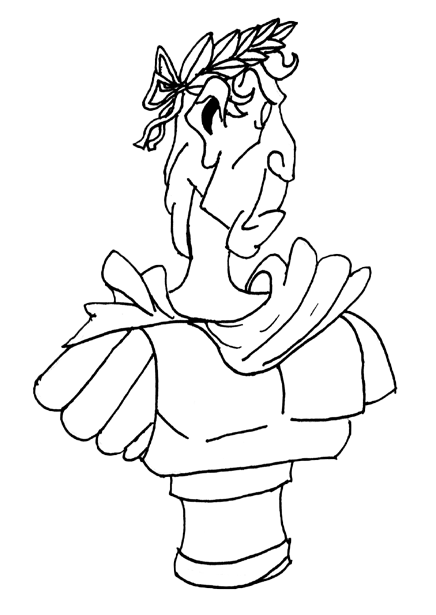
\includegraphics[height=5cm, right]{images/lekcja_historii_klasycznej.png}\vspace*{-5.05cm}\\
  Nad Europą twardy krok legionów grzmi\\
  Nieunikniony wróży koniec republiki\\
  Gniją wzgórza galijskie w pomieszanej krwi\\
  A Juliusz Cezar pisze swoje pamiętniki\\
  \\
  Pozwól, Cezarze, gdy zdobędziemy cały świat\\
  Gwałcić, rabować, sycić wszelkie pożądania\\
  Proste prośby żołnierzy te same są od lat\\
  A Juliusz Cezar milcząc, zabaw nie zabrania\\
  \\
  Cywilizuje podbite narody w nowy ład\\
  Rosną krzyże przy drogach od Renu do Nilu\\
  Skargą, krzykiem i płaczem rozbrzmiewa cały świat\\
  A Juliusz Cezar ćwiczy lapidarność stylu\\
\end{minipage}
\begin{minipage}[t]{0.2\textwidth}
  E H\\
  fis Gis\\
  cis A\\
  E H (E A E H)\\

  E H\\
  fis Gis\\
  cis A\\
  E H (E A E H)\\

  E H\\
  fis Gis\\
  cis A\\
  E H (E A E H)\\

  E H\\
  fis Gis\\
  cis A\\
  E H (E A E H)\\
\end{minipage}

\newpage
\section{Lemon tree}\textcolor{lightgray}{\textit{Fool's Garden}}\\~\\
\begin{minipage}[t]{0.8\textwidth}
  I'm sitting here, in a boring room \\
  It's just another rainy sunday afternoon\\
  I'm wasting my time, I got nothing to do\\
  I'm hanging around, I'm waiting for you\\
  But nothing ever happens - and I wonder\\

  I'm driving around in my car\\
  I'm driving too fast, I'm driving too far\\
  I'd like to change my point of view\\
  I feel so lonely, I'm waiting for you\\
  But nothing ever happens - and I wonder\\

  \hspace*{5mm}I wonder how, I wonder why\\
  \hspace*{5mm}Yesterday you told me 'bout the blue blue sky \\
  \hspace*{5mm}And all that I can see is just a yellow lemon tree\\

  \hspace*{5mm}I'm turning my head up and down\\
  \hspace*{5mm}I'm turning turning turning turning turning around\\
  \hspace*{5mm}And all that I can see is just another lemon tree\\

  I'm sitting here, I miss the power \\
  I'd like to go out, taking a shower\\
  But there's heavy cloud inside my head\\
  I feel so tired, put myself into bed\\
  Where nothing ever happens - and I wonder \\

  \hspace*{3mm}Isolation is not good for me\\
  \hspace*{3mm}Isolation, I don't want to sit on a lemon tree \\

  I'm steppin' around in a desert of joy\\
  Baby, anyhow I'll get another toy\\
  And everything will happen - and you'll wonder\\

\end{minipage}
\begin{minipage}[t]{0.2\textwidth}
  fis cis\\
  fis cis\\
  fis cis\\
  fis cis\\
  h cis fis\\

  fis cis\\
  fis cis\\
  fis cis\\
  fis cis\\
  h cis fis\\

  A E\\
  fis cis\\
  D E A (E)\\

  A E\\
  fis cis\\
  D H7 E\\

  fis cis\\
  fis cis\\
  fis cis\\
  fis cis\\
  h cis fis\\


  Cis fis\\
  E A Cis\\

  fis cis\\
  fis cis\\
  h cis fis\\


\end{minipage}

\newpage
\section{Locomotive Breath}\textcolor{lightgray}{\textit{Jethro Tull}}\\~\\
\begin{minipage}[t]{0.8\textwidth}
  In the shuffling madness\\
  Of the locomotive breath\\
  Runs the all-time loser\\
  Headlong to his death\\
  Oh, he feels the piston scraping\\
  Steam breaking on his brow\\
  Old Charlie stole the handle\\
  And the train it won't stop\\
  Oh no way to slow down\\

  He sees his children jumping off\\
  At the stations one by one\\
  His woman and his best friend\\
  In bed and having fun\\
  Oh, he's crawling down the corridor\\
  On his hands and knees\\
  Old Charlie stole the handle\\
  And the train it won't stop going\\
  No way to slow down\\

  He hears the silence howling\\
  Catches angels as they fall\\
  And the all-time winner\\
  Has got him by the balls\\
  Oh, he picks up Gideons bible\\
  Open at page one\\
  I think God he stole the handle\\
  And the train it won't stop going\\
  No way to slow down\\

  No way to slow down \hspace*{10mm}$\times$8\\
\end{minipage}
\begin{minipage}[t]{0.2\textwidth}
  e G D e\\
  e G D e\\
  e D G H\\
  H H D e\\
  e G D e\\
  e G D\\
  G A\\
  H\\
  H H D e\\

  e G D e\\
  e G D e\\
  e D G H\\
  H H D e\\
  e G D e\\
  e G D\\
  G A\\
  H\\
  H H D e\\

  e G D e\\
  e G D e\\
  e D G H\\
  H H D e\\
  e G D e\\
  e G D\\
  G A\\
  H\\
  H H D e\\
\end{minipage}

\newpage
\section{Long as I can see the light}\textcolor{lightgray}{\textit{Creedence Clearwater Revival}}\\~\\
\begin{minipage}[t]{0.8\textwidth}
  Put a candle in the window\\
  ‘Cause I feel I've got to move\\
  Though I'm going, going, I'll be coming home soon\\
  'Long as I can see the light\\
  \\
  Pack my bag and let's get movin'\\
  ‘Cause I'm bound to drift a while\\
  When I'm gone, gone, you don't have to worry long\\
  'Long as I can see the light.\\
  \\
  Guess I've got that old trav'lin' bone\\
  ‘Cause this feelin' won't leave me alone\\
  But I won't, won't be losin' my way, no, no\\
  'Long as I can see the light\\
\end{minipage}
\begin{minipage}[t]{0.2\textwidth}
  H Fis H\\
  H gis H Fis\\
  H Fis E\\
  H Fis H\\

  H Fis H\\
  H gis H Fis\\
  H Fis E\\
  H Fis H\\

  H Fis H\\
  H gis H Fis\\
  H Fis E\\
  H Fis H\\
\end{minipage}
\vfill
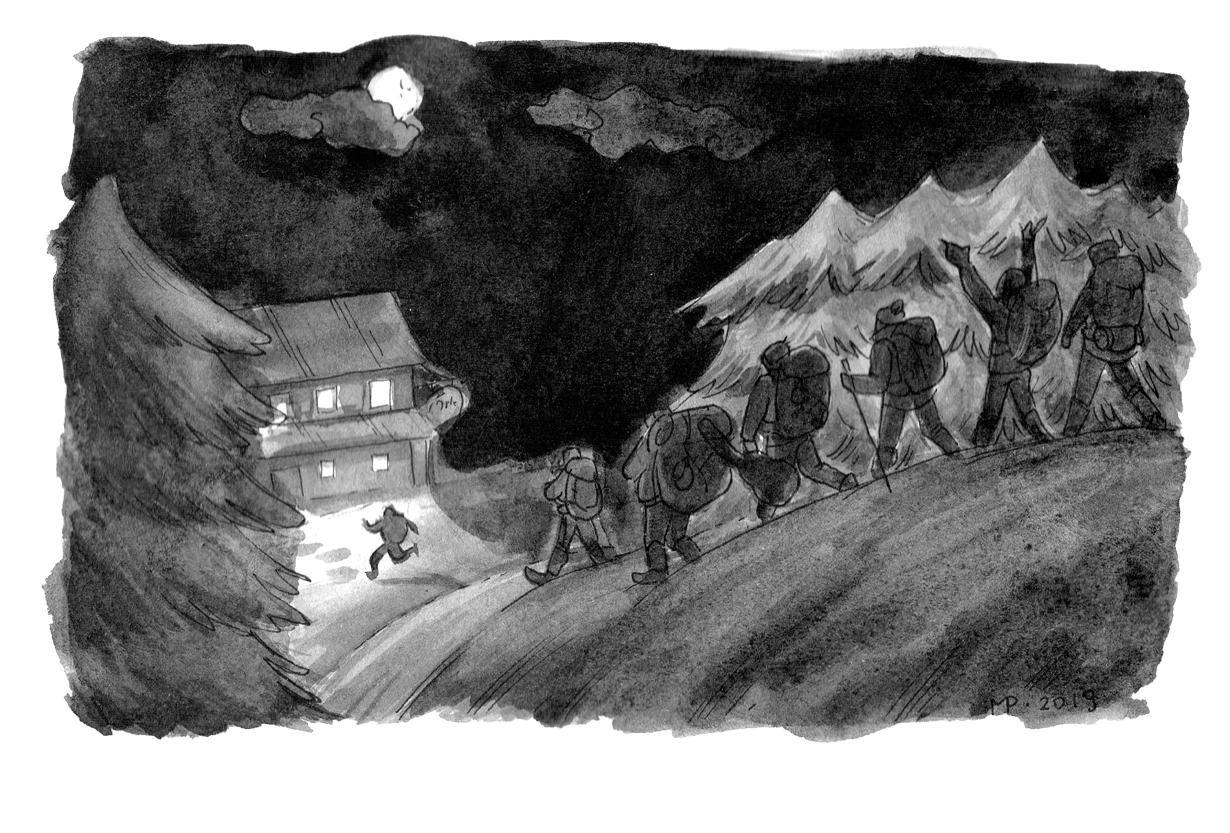
\includegraphics[width=\textwidth, center]{images/long_as_i_can_see_the_light.png}\\

\newpage
\section{Lornetka}\textcolor{lightgray}{\textit{Golec uOrkiestra}}\\~\\
\begin{minipage}[t]{0.75\textwidth}
  Kupiłek lornetke, by podglondać Bernadetke\\
  Ale w łoknak żaluzje mo zasłonięte\\
  Księżyc wisi na niebie a jo wciąs nie widzem ciebie\\
  Marzem, coby ryntgenem być w takiej chwili\\
  \\
  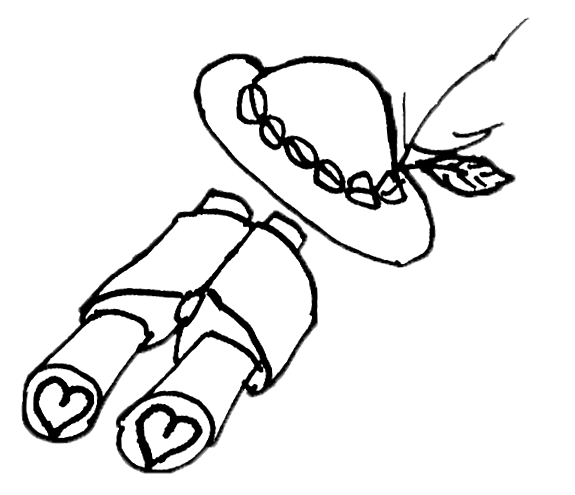
\includegraphics[height=2cm, right]{images/lornetka.png}\vspace*{-2.05cm}\\
  \hspace*{5mm}Tak bardzo, bardzo kochom jom\\
  \hspace*{5mm}Że w nocy, kiedy wszyscy śpiom\\
  \hspace*{5mm}Jo nie śpie, kombinując jak być z niom\\
  \\
  Cekołbyk do rana, lec matuś zdenerwowana\\
  Krzycy: znowu nie wstanies na piyrsom zmiane\\
  Ale matuś nie wie o tym, że kierownik mnie z roboty\\
  Wyloł, bo miołek problemy wciąs z koncentrancjom.\\
  \\
  Wcoraj wpod mi do głowy pomysł cołkiem łodlotowy\\
  Że jej wyślem miłosny list anonimowy\\
  Myślem sobie łokradkiem: może kasik psypadkiem\\
  Biegnąc psepadnie, wpadając wprost w me ramiona\\
\end{minipage}
\begin{minipage}[t]{0.25\textwidth}
  C E E$^7$ F d\\
  B G$^7$ C E$^7$\\
  C E E$^7$ F d\\
  B G$^7$ C E$^7$\\

  F G\\
  C a\\
  F d G C (E$^7$)\\
  \\
  C E E$^7$ F d\\
  B G$^7$ C E$^7$\\
  C E E$^7$ F d\\
  B G$^7$ C E$^7$\\

  C E E$^7$ F d\\
  B G$^7$ C E$^7$\\
  C E E$^7$ F d\\
  B G$^7$ C E$^7$\\

\end{minipage}
\vfill
% \newpage
\section{Lubię mówić z tobą}\textcolor{lightgray}{\textit{Akurat}}\\~\\
\begin{minipage}[t]{0.8\textwidth}
  Kiedy z serca płyną słowa, uderzają z wielką mocą\\
  Krążą blisko wśród nas, ot tak, dając chętnym szczere złoto\\
  \\
  \hspace*{5mm}I dlatego lubię mówić z tobą\\
  \\
  Każdy myśli to co myśli, myśli sobie moja głowa\\
  Może w końcu mi się uda wypowiedzieć proste słowa\\
\end{minipage}
\begin{minipage}[t]{0.2\textwidth}
  cis E H cis\\
  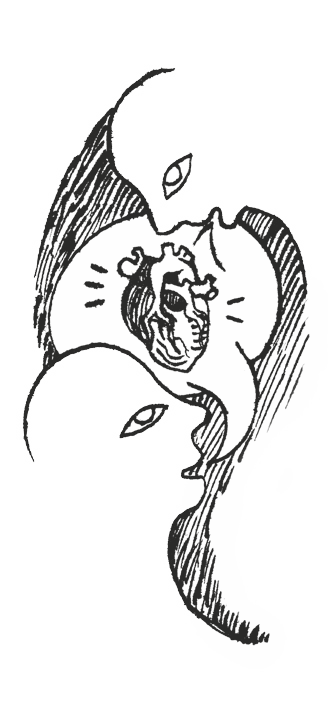
\includegraphics[width=0.9\textwidth]{images/lubie_mowic_z_toba.png}\\

\end{minipage}

\newpage
\section{Majster Bieda}\textcolor{lightgray}{\textit{WGB}}\\~\\
\begin{minipage}[t]{0.7\textwidth}
  ~\\
  Skąd przychodził, kto go znał\\
  Kto mu rękę podał, kiedy\\
  Nad rowem siadał, wyjmował chleb\\
  Serem przekładał i dzielił się z psem\\
  Tyle wszystkiego, co z sobą miał\\
  Majster Bieda\\
  \\
  Czapkę z głowy ściągał, gdy\\
  Wiatr gałęzie chylił drzewom\\
  Śmiał się do słońca i śpiewał do gwiazd\\
  Drogę bez końca co przed nim szła\\
  Znał jak pięć palców, jak szeląg zły\\
  Majster Bieda\\
  \\
  Nikt nie pytał, skąd się wziął\\
  Gdy do ognia się przysiadał\\
  Wtulał się w krąg ciepła, jak w kożuch\\
  Znużony drogą wędrowiec boży\\
  Zasypiał długo gapiąc się w noc\\
  Majster Bieda\\
  \\
  Aż nastąpił taki rok\\
  Smutny rok, tak widać trzeba\\
  Nie przyszedł Bieda zieloną wiosną\\
  Miejsce, gdzie siadał, zielskiem zarosło\\
  I choć niejeden wytężał wzrok\\
  Choć lato pustym gościńcem przeszło\\
  Z rudymi liśćmi, jesieni schedą\\
  Wiatrem niesiony popłynął w przeszłość\\
  Majster Bieda\\
\end{minipage}
\begin{minipage}[t]{0.3\textwidth}
  (D G fis e A D)\\
  D G\\
  D G A\\
  D A\\
  fis h\\
  A G (fis e)\\
  A D\\

  D G\\
  D G A\\
  D A\\
  fis h\\
  A G (fis e)\\
  A D\\

  D G\\
  D G A\\
  D A\\
  fis h\\
  A G (fis e)\\
  A D\\

  D G\\
  D D$^7$ G A\\
  D A\\
  fis h\\
  A G\\
  A G\\
  A G\\
  A G (A)\\
  D G fis e A D\\
\end{minipage}

\newpage
\section{Małgośka}\textcolor{lightgray}{\textit{Maryla Rodowicz}}\\~\\
\begin{minipage}[t]{0.85\textwidth}
  To był maj, pachniała Saska Kępa szalonym zielonym bzem\\
  To był maj, gotowa była ta sukienka i noc się stawała dniem\\
  Już zapisani byliśmy w urzędzie, białe koszule na sznurze schły\\
  Nie wiedziałam, co ze mną będzie\\
  Gdy tamtą dziewczynę pod rękę ujrzałam z nim\\
  \\
  \hspace*{6mm}Małgośka, mówią mi, on nie wart jednej łzy\\
  \hspace*{6mm}On nie jest wart jednej łzy (oj, głupia!)\\
  \hspace*{6mm}Małgośka, wróżą z kart, on nie jest grosza wart\\
  \hspace*{6mm}Ach, weź go czart, weź go czart\\

  \hspace*{6mm}Małgośka, tańcz i pij, a z niego sobie kpij\\
  \hspace*{6mm}A z niego kpij sobie, kpij (oj, głupia!)\\
  \hspace*{6mm}Jak wróci, powiedz: nie, niech zginie gdzieś na dnie\\
  \hspace*{6mm}Ej, głupia ty, głupia ty, głupia ty\\
  \\
  Jesień już, już pachną chwasty w sadach i pachnie zielony dym\\
  Jesień już, gdy zajrzę do sąsiada, pytają mnie, czy jestem z nim\\
  Widziałam biały ślub, idą święta, nie słyszałam z daleka słów\\
  Może rosną im już pisklęta\\
  A suknia tej młodej uszyta jest z moich snów\\
  \\
\end{minipage}
\begin{minipage}[t]{0.15\textwidth}
  a\\
  F a\\
  E a\\
  F a\\
  D$^7$ G G$^7$\\

  C a\\
  C G\\
  a F\\
  a  D$^7$\\

  C a\\
  C G\\
  a F\\
  a  D$^7$\\

  a\\
  F a\\
  E a\\
  F a\\
  D$^7$ G G$^7$\\
\end{minipage}

% \newpage
\section{Marchewkowe Pole}\textcolor{lightgray}{\textit{Lady Pank}}\\~\\
\begin{minipage}[t]{0.7\textwidth}
  Marchewkowe pole rośnie wokół mnie \\
  W marchewkowym polu jak warzywo tkwię \\
  Głową na dół zakopany niczym struś \\
  Chcesz mnie spotkać, głowę obok w ziemię wpuść \\
  \\
  \hspace*{5mm}Wszystko się może zdarzyć \hspace*{10mm} $\times$2\\
  \\
  Marchewkowe o ogrodzie miewam sny \\
  W marchewkowym stanie jest najlepiej mi \\
  Rosnę sobie dołem głowa górą nać \\
  Kto mi powie co się jeszcze może stać\\

  \hspace*{5mm}Wszystko się może zdarzyć \hspace*{10mm} $\times$4\\
\end{minipage}
\begin{minipage}[t]{0.3\textwidth}
  D A F G D\\
  D A F G D\\
  D A F G D\\
  D A F G D\\

  D A e F G\\

  D A F G D\\
  D A F G D\\
  D A F G D\\
  D A F G D\\

  D A e F G\\
\end{minipage}

\newpage
\section{Mgła}\textcolor{lightgray}{\textit{}}\\~\\
\begin{minipage}[t]{0.8\textwidth}
  Mgła okryła domy i ulice\\
  Wpełzła w szpary między okiennice\\
  Ja w pokoju siedzę, a za oknem\\
  Dzieją się tam rzeczy przeokropne\\
  \\
  Mgła... $\times$4\\
  \\
  Patrzę, a tam przy cmentarnej bramie\\
  Kat jakiegoś gościa kołem łamie\\
  Kat nad gościem męczy się i poci\\
  Ludzie patrzą, czyżby kat robotę sknocił?\\
  Kat straszliwe śruby swe dokręca\\
  Już nad gościem nie ma siły się znęcać\\
  Nagle w tłumie słychać skargę gościa\\
  Jejku, jak mnie dzisiaj łamie w kościach\\
  \\
  Patrzę, a tam zaraz za zakrętem\\
  Wampir jakąś babkę dusi prętem\\
  Taka kolej rzeczy już być musi\\
  Wampir jedną babkę w roku musi zdusić\\
  Czemu dzisiaj babkę tę przypierasz?\\
  Pytam grzecznie damskiego wampira\\
  Czemu dzisiaj brudzisz swe paluszki?\\
  Jak to? Przecież właśnie dzisiaj są Zaduszki\\
  \\
  Tam na plantach, tuż obok cmentarza\\
  Mąż żonie wrzątkiem gębę wyparza\\
  Chyba pójdę tam ze swoją żoną\\
  Ona także gębę ma niewyparzoną\\
  \\
  Jedna baba drugiej takiej babie\\
  Wsadziła do torby grabie\\
  A poza tym całkiem jeszcze nową\\
  Wsadziła jej w torbę bombę atomową\\
  Teraz zaś niejaki pan Drakula\\
  Babkę z bombą w torbie gdzieś przytula\\
  Wampir wiele kobiet ma w rezerwie\\
  Lecz ta babka świetnie przecież go rozerwie\\
\end{minipage}
\begin{minipage}[t]{0.2\textwidth}
  a F E\\
\end{minipage}

\newpage
\section{Mijają cztery pory roku}\textcolor{lightgray}{\textit{Janusz Laskowski}}\\~\\
\begin{minipage}[t]{0.8\textwidth}
  Była jesień, przyszła w ciemnej sukience\\
  Jeden uśmiech, jak wspomnienie lata\\
  \hspace*{5mm}Szła z walizką, stanęła na piętrze\\
  \hspace*{5mm}Był jej domem akademik stary\\
  \\
  Przyszła zima i były zawieje\\
  Płatki śniegu nosiła we włosach\\
  \hspace*{5mm}Był sylwester spędzany we dwoje\\
  \hspace*{5mm}Strzał szampana obudził nadzieję\\
  \\
  Potem wiosna i inne nastroje\\
  Nowy semestr, wspólne plany były\\
  \hspace*{5mm}Mały pokój znalazłem na mieście\\
  \hspace*{5mm}I śpiewaniem żywiłem nas dwoje\\
  \\
  Wreszcie lato, kwiatami pachniało\\
  Zabrał rzeczy przepełniony pociąg\\
  \hspace*{5mm}Potem cisza, tylko radio grało\\
  \hspace*{5mm}I wspomnienie tej jesieni zostało\\
\end{minipage}
\begin{minipage}[t]{0.2\textwidth}
  E a \\
  G a \\
  d G C\\
  E a \\

  E a \\
  G a \\
  d G C\\
  E a \\

  E a \\
  G a \\
  d G C\\
  E a \\

  E a \\
  G a \\
  d G C\\
  E a \\
\end{minipage}

\newpage
\section{Milczenie owiec}\textcolor{lightgray}{\textit{Zioma}}\\~\\
\begin{minipage}[t]{0.8\textwidth}
  Za lasem, za górą - Za górą, za lasem\\
  Żyli se we dwoje, w chałupie oboje\\
  Dziewucha z juhasem\\
  \\
  On roz łowiecki wziął - On wziął łowiecki roz\\
  I pedział jej chmurnie: Idę ja na turnie\\
  Będę ci owce posł\\
  \\
  A ledwie wzeszła noc - A ledwie noc wzeszła\\
  Owieczkę se wybroł, do naga ostrzygnął\\
  I wziął do szałasa\\
  \\
  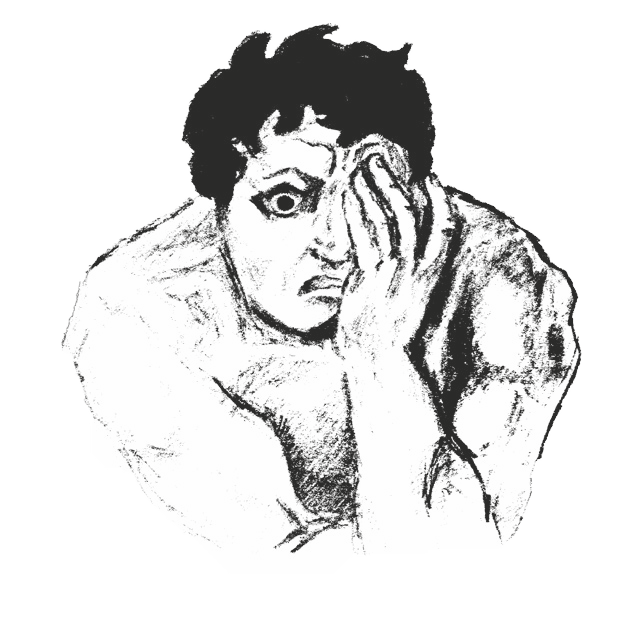
\includegraphics[height=3cm, right]{images/milczenie_owiec.png}\vspace*{-3.05cm}\\
  A dziewczyna jego - A jego dziewczyna\\
  W samym środku nocy otwarła swe oczy\\
  Przeczuciem targniona\\
  \\
  Chuścinę wzięła swą - Chuścinę swą wzięła\\
  Przez percie wysokie, wądoły głębokie\\
  Za chłopem pognała\\
  \\
  Przecudny świt wstowoł - Przecudny wstowoł świt\\
  Gdy wyjszła spod lasa, wtargła do szałasa\\
  I rozległ się jej krzyk (aaa!)\\
  \\
  O ty sodomito - O sodomito ty\\
  Już dość tych igraszek, wnet zmilknie twój ptaszek\\
  Zapłacisz za me łzy\\
  \\
  I bierze fest kozik - I bierze kozik fest\\
  Ptok frunie na ziemię, krew tryska strumieniem\\
  I horror, fajno jest\\
  \\
  A morał taki z tej straszliwej ballady\\
  Potwierdzić to mogę, trza kochać przyrodę\\
  Ale bez przesady\\
\end{minipage}
\begin{minipage}[t]{0.2\textwidth}
  a e a e $/\times$2\\
  a e a d\\
  a e a e\\

  a e a e $/\times$2\\
  a e a d\\
  a e a e\\

  a e a e $/\times$2\\
  a e a d\\
  a e a e\\

  a e a e $/\times$2\\
  a e a d\\
  a e a e\\

  a e a e $/\times$2\\
  a e a d\\
  a e a e\\

  a e a e $/\times$2\\
  a e a d\\
  a e a e\\

  a e a e $/\times$2\\
  a e a d\\
  a e a e\\

  a e a e $/\times$2\\
  a e a d\\
  a e a e\\

  a e a e $/\times$2\\
  a e a d\\
  a e a e\\
\end{minipage}

\newpage
\section{Mniej niż zero}\textcolor{lightgray}{\textit{Lady Pank}}\\~\\
\begin{minipage}[t]{0.8\textwidth}
  O o o o $\times 4$\\
  \\
  Myślisz może, że więcej coś znaczysz\\
  Bo masz rozum, dwie ręce i chęć\\
  Twoje miejsce na Ziemi tłumaczy\\
  Zaliczona matura na pięć\\
  Są tacy - to nie żart\\
  Dla których jesteś wart\\
  \\
  Mniej niż zero $\times 4$\\
  O o o o $\times 4$\\
  \\
  Zawodowi macherzy od losu\\
  Specjaliści od śpiewu i mas\\
  Choćbyś nie chciał i tak znajdą sposób\\
  Na swej wadze położą nie raz\\
  Choć to fizyce wbrew\\
  Wskazówka cofa się\\
  \\
  Myślisz może, że więcej coś znaczysz\\
  Bo masz rozum, dwie ręce i chęć\\
  Twoje miejsce na Ziemi tłumaczy\\
  Zaliczona matura na pięć\\
  Są tacy - to nie żart\\
  Dla których jesteś wart\\
\end{minipage}
\begin{minipage}[t]{0.2\textwidth}
  DDDe\\~\\e D\\e D\\e D\\e D\\C D\\C D\\
  ~\\e D\\
  DDDe\\~\\
  e D\\e D\\e D\\e D\\C D\\C D\\

  e D\\e D\\e D\\e D\\C D\\C D\\
\end{minipage}

\newpage
\section{Moja i twoja nadzieja}\textcolor{lightgray}{\textit{Hey}}\\~\\
\begin{minipage}[t]{0.8\textwidth}
  Spróbuj powiedzieć to, nim uwierzysz, że\\
  Nie warto mówić kocham\\
  Spróbuj uczynić gest, nim uwierzysz, że\\
  Nic nie warto robić\\

  \hspace*{7mm}Nic, naprawdę nic nie pomoże\\
  \hspace*{7mm}Jeśli ty nie pomożesz dziś miłości\\
  \\
  Musisz odnaleźć nadzieję i nieważne, że\\
  Nazwą ciebie głupcem\\
  Musisz pozwolić, by sny\\
  Sprawiły byś pamiętał, że\\

  \hspace*{3mm}Moja i twoja nadzieja\\
  \hspace*{3mm}Uczyni realnym krok w chmurach\\
  \hspace*{3mm}Moja i twoja nadzieja\\
  \hspace*{3mm}Pozwoli uczynić dziś cuda\\
\end{minipage}
\begin{minipage}[t]{0.2\textwidth}
  a G d a G\\
  d\\
  a G d a G\\
  d\\

  a G d\\
  a G d\\

  a G d a G\\
  d\\
  a G d a G\\
  d\\

  a G F G\\
  a G F G\\
  a G F G\\
  a G F G\\

\end{minipage}

\newpage
\section{Moja litania}\textcolor{lightgray}{\textit{Leszek Wójtowicz}}\\~\\
\begin{minipage}[t]{0.8\textwidth}
  Jaki jeszcze mi numer wytniesz\\
  W którą ślepą skierujesz ulicę\\
  Ile razy palce sobie przytnę\\
  Nim się wreszcie klamki uchwycę\\
  By otworzyć drzwi do Twego serca\\
  Które przeszło już tyle zawałów\\
  Czy nikogo więcej nie obudzą\\
  W Twym imieniu oddane wystrzały\\
  \\
  \hspace*{5mm}Nie pragnę wcale, byś była wielka\\
  \hspace*{5mm}Zbrojna po zęby od morza do morza\\
  \hspace*{5mm}I nie chcę także, by Cię uważano\\
  \hspace*{5mm}Za perłę świata i wybrankę Boga\\
  \hspace*{5mm}Chcę tylko domu w Twoich granicach\\
  \hspace*{5mm}Bez lokatorów stukających w ściany\\
  \hspace*{5mm}Gdy ktoś chce trochę głośniej zaśpiewać\\
  \hspace*{5mm}O sprawach, które wszyscy dobrze znamy\\
  \\
  Jakim ludziom jeszcze pozwolisz\\
  By Twym mózgiem byli i sumieniem\\
  Kto z przyjaciół pokaże mi blachy\\
  Kładąc rękę na moim ramieniu\\
  Czy Twój język nadal pozostanie\\
  Arcyszyfrem nie do rozwiązania\\
  Czy naprawdę zaczęłaś odpowiadać\\
  Na najprostsze zadane pytania\\
  \\
  Ile razy swoją twarz ukryjesz\\
  Za zasłoną flag i transparentów\\
  Ile lat będziesz mi przypominać\\
  Rozpędzony burzą wrak okrętu\\
  Tą litanią się do Ciebie modlę\\
  Bardzo bliska jesteś i daleka\\
  Ale jest coś takiego w Tobie\\
  Że pomimo wszystko wierzę, czekam\\
\end{minipage}
\begin{minipage}[t]{0.2\textwidth}
  a\\
  d\\
  G\\
  C E\\
  a\\
  d\\
  G\\
  C E\\

  a d\\
  G C E\\
  a d\\
  G C E\\
  a d\\
  G C E\\
  a d\\
  G C E\\

  a\\
  d\\
  G\\
  C E\\
  a\\
  d\\
  G\\
  C E\\

  a\\
  d\\
  G\\
  C E\\
  a\\
  d\\
  G\\
  C E\\
\end{minipage}

\newpage
\section{Mój jest ten kawałek podłogi}\textcolor{lightgray}{\textit{Mr Zoob}}\\~\\
\begin{minipage}[t]{0.6\textwidth}
  Znowu ktoś mnie podgląda\\
  Lekko skrobie do drzwi\\
  Strasznym okiem cyklopa\\
  Radzi, gromi i drwi!\\

  \hspace*{5mm}Mój jest ten kawałek podłogi\\
  \hspace*{5mm}Nie mówcie mi więc, co mam robić!\\

  Meble już połamałem\\
  Nowy ład zrobić chcę\\
  Tynk ze ścian już zdrapałem\\
  Zamurować czas drzwi!\\

  Wielkie dzieło skończyłem\\
  But do wyjścia mnie pcha\\
  Prężę się i napinam\\
  Lecz mur stoi jak stał\\

\end{minipage}
\begin{minipage}[t]{0.4\textwidth}
  h G A (h)\\
  \\
  \\
  \\
  \\
  D A h G\\
  \\
  (A)\\
  h G A (h)\\
  \\
  \\
  \\
  \\
  h G A (h)\\
  \\
  \\
  \\
  \\
\end{minipage}

\newpage
\section{Mój przyjacielu}\textcolor{lightgray}{\textit{Krzysztof Krawczyk}}\\~\\
\begin{minipage}[t]{0.7\textwidth}
  Mój przyjacielu, byłeś mi naprawdę bliski\\
  Mój przyjacielu, wiesz, że byłeś mi, jak brat\\
  Dałem Ci wiarę, dałem Ci spokój\\
  Dałem gitarę, dałem samochód\\
  I dach nad głową, a do sypialni wszedłeś sam\\

  Mój przyjacielu, przyprowadziłem Cię z ulicy\\
  Nakarmiłem i odziałem Cię, jak brat\\
  Dałem Ci wiarę, dałem Ci spokój\\
  Dałem gitarę, dałem samochód\\
  Żony nie dałem, żonę wziąłeś sobie sam\\

  \hspace*{3mm}Teraz pijesz wino, pijesz aż do dna\\
  \hspace*{3mm}Późna już godzina, próżno czekasz dnia\\
  \hspace*{3mm}Chciałbyś się rozpłynąć, uciec, gdzie się da\\
  \hspace*{3mm}Proszę zostań na noc, przyjaźń swoje prawa ma\\

  \hspace*{3mm}Teraz pijesz wino, pijesz aż do dna\\
  \hspace*{3mm}Późna już godzina, próżno czekasz dnia\\
  \hspace*{3mm}Chciałbyś się rozpłynąć, uciec, gdzie się da\\
  \hspace*{3mm}Może spać spokojnie, kto przyjaźni prawa zna\\

  Mój przyjacielu, jak wyrazić to, co czuję\\
  Jak wytłumaczyć, czym jest dla mnie przyjaźń Twa\\
  Dałem Ci wiarę, dałem Ci spokój\\
  Dałem gitarę, dałem samochód\\
  Żony nie dałem, żonę wziąłeś sobie sam\\
\end{minipage}
\begin{minipage}[t]{0.3\textwidth}
  a E$^7$ a\\
  C G C\\
  F C\\
  F C\\
  E (E$^7$) a\\

  a E$^7$ a\\
  C G C\\
  F C\\
  F C\\
  E (E$^7$) a\\

  G G$^7$ C\\
  G G$^7$ C\\
  G F C\\
  E a\\

  G G$^7$ C\\
  G G$^7$ C\\
  G F C\\
  E a\\

  a E$^7$ a\\
  C G C\\
  F C\\
  F C\\
  E (E$^7$) a
\end{minipage}
\includegraphics[width=0.5\textwidth, center]{images/moj_przyjacielu.png}\\

\newpage
\section{Muszka Plujka}\textcolor{lightgray}{\textit{Wały Jagiellońskie}}\\~\\
\begin{minipage}[t]{0.8\textwidth}
  Muszka plujka i żuczek gnojarek 					\\
  Stanowili razem dość dobraną parę					\\
  Ona była plujka, a on zwykły żuk					\\
  I żyli szczęśliwie, choć mu brakło nóg				\\
  \\
  Muszka plujka i żuczek gnojarek\\
  Co dzień rano wokół krowiej kupki odprawiali bale\\
  Ona była plujka, a on nie miał wujka\\
  A na dodatek nie miał nóg ten żuk\\
  \\
  Muszka plujka i gnojarek żuczek\\
  Ona była wierna, on miał jeszcze parę innych suczek\\
  Miłosnej euforii szybko mijał czas\\
  Lecz trwało to krótko, bo zabił ich gaz\\
  \\
  Taka to historia, smutna, lecz prawdziwa\\
  Ona była plujka, a on stary dziwak\\
  Lecz skąd gaz, pytacie, cień się plujki błąka\\
  Tak, to słoń zawinił, bo drań… bo drań\\
\end{minipage}
\begin{minipage}[t]{0.2\textwidth}
  a E \\
  E a \\
  a d \\
  a E a\\

  a E \\
  E a \\
  a d \\
  a E a\\

  a E \\
  E a \\
  a d \\
  a E a\\

  a E \\
  E a \\
  a d \\
  a E a\\
\end{minipage}

\newpage
\section{My cyganie}\textcolor{lightgray}{\textit{Krzysztof Krawczyk}}\\~\\
\begin{minipage}[t]{0.7\textwidth}
  My, Cyganie, co pędzimy z wiatrem\\
  My, Cyganie, znamy cały świat\\
  My, Cyganie, wszystkim gramy\\
  A śpiewamy sobie tak\\
  \\
  \hspace*{6mm}Ore, ore, szabadabada amore\\
  \hspace*{6mm}Hej, amore szabadabada\\
  \hspace*{6mm}O muriaty, o szagriaty\\
  \hspace*{6mm}Hajda trojka na mienia\\
  \\
  Kiedy tańczę, niebo tańczy razem ze mną\\
  Kiedy gwiżdżę, gwiżdże ze mną wiatr\\
  Zamknę oczy, liście więdną\\
  Kiedy milknę, milczy świat\\
  \\
  Gdy śpiewamy, słucha cała Ziemia\\
  Gdy śpiewamy, słucha cały świat\\
  Niechaj każdy z nami śpiewa\\
  Niech rozbrzmiewa piosnka ta\\
  \\
  Będzie prościej, będzie jaśniej\\
  Całą radość damy wam\\
  Będzie prościej, będzie jaśniej\\
  Gdy zaśpiewa każdy z was\\
\end{minipage}
\begin{minipage}[t]{0.3\textwidth}
  F C\\
  d a\\
  d a\\
  E$^7$ a A\\

  F C\\
  d a\\
  d a\\
  E$^7$ a A\\

  F C\\
  d a\\
  d a\\
  E$^7$ a A\\

  F C\\
  d a\\
  d a\\
  E$^7$ a A\\

  F C\\
  d a\\
  d a\\
  E$^7$ a A\\
\end{minipage}

% \newpage
\section{Na jednej z dzikich plaż}\textcolor{lightgray}{\textit{Rotary}}\\~\\
\begin{minipage}[t]{0.8\textwidth}
  Samochód w deszczu stał\\
  Radio przestało grać\\
  Dotknąłem kolan twych\\
  Nie liczyliśmy gwiazd.\\
  \\
  \hspace*{5mm}Lubiła tańczyć pełna radości tak ciągle goniła wiatr\\
  \hspace*{5mm}Spragniona życia wciąż zawsze gubiła coś nie chciała nic\\
  \hspace*{5mm}Nie rozumiałem kiedy mówiła mi: "Dzisiaj ostatni raz\\
  \hspace*{5mm}Zatańczmy proszę tak jak gdyby umarł czas." Mówiła mi\\
  \\
  Mieliśmy wiecznie trwać\\
  Na jednej z dzikich plaż\\
  Chciałem ze wszystkich sił\\
  Pozostać z Tobą tam\\
\end{minipage}
\begin{minipage}[t]{0.2\textwidth}
  C a\\
  ~\\
  ~\\
  ~\\
  ~\\
  F G e a\\
\end{minipage}

\newpage
\section{Na włóczęgę}\textcolor{lightgray}{\textit{Bułat Okudżawa}}\\~\\
\begin{minipage}[t]{0.82\textwidth}
  Na włóczęgę już wyruszyć przyszła pora\\
  Las nas woła śpiewem ptaków, szumem drzew\\
  I wołają nas już pola i jeziora\\
  Zeszłoroczny nasz, wesoły pomnąc śpiew\\
  \hspace*{5mm}Ludzie mają swoje prace, ludzie lubią się bogacić\\
  \hspace*{5mm}Pełne brzuchy mają, chcą mieć pełen trzos\\
  A ja gonię, a ja gonię swe marzenia\\
  Szczęścia szukam, gdzie kaczeńce i gdzie wrzos\\
  \\
  Tym, co iść nie lubią, mówię: Do widzenia\\
  Za dni kilka pewnie znów powrócę tu\\
  Idę w świat, by tam dogonić swe marzenia\\
  Aby spełnić kilka moich złotych snów\\
  \hspace*{5mm}Więc z dziewczyną swą pod rękę i z gitarą i z piosenką\\
  \hspace*{5mm}Precz mi smutki, precz przykrości - słońce, świeć!\\
  Idę gonić, idę gonić swe marzenia\\
  I spokoju szukać pośród starych drzew\\
  \\
  Tak to proste, że i gadać szkoda czasu\\
  Tylko plecak wziąć i iść przed siebie wprost\\
  Szukać wiatru i zapachu szukać lasu\\
  Jak najdalej zadymionych wielkich miast\\
  \hspace*{5mm}Zrozum, bracie, to tak trzeba - łóżkiem trawa, dachem drzewa\\
  \hspace*{5mm}Z wiatrem biegać i z ptakami śpiewać w głos\\
  Trzeba gonić, trzeba gonić swe marzenia\\
  A nie czekać, ile trosk przyniesie los\\
  \\

\end{minipage}
\begin{minipage}[t]{0.18\textwidth}
  e a\\
  H$^7$ e (H$^7$)\\
  e a\\
  H$^7$ e\\
  E a\\
  D$^7$ G H$^7$\\
  e a\\
  H$^7$ e (H$^7$)\\

  e a\\
  H$^7$ e (H$^7$)\\
  e a\\
  H$^7$ e\\
  E a\\
  D$^7$ G H$^7$\\
  e a\\
  H$^7$ e (H$^7$)\\

  e a\\
  H$^7$ e (H$^7$)\\
  e a\\
  H$^7$ e\\
  E a\\
  D$^7$ G H$^7$\\
  e a\\
  H$^7$ e (H$^7$)\\
\end{minipage}

\newpage
\section{Nadzieja / Sweet home Alabama}~\\~\\
\begin{minipage}[t]{0.8\textwidth}
  Możesz masz w głowie myśli bardziej szalone niż ja\\
  Może masz skrzydła, których by tobie pozazdrościł ptak\\
  Może masz serce całe ze szlachetnego szkła\\
  Może masz kogoś, a może właśnie kogoś ci brak\\
  \\
  \hspace*{5mm}Nie ma nikt takiej nadziei, jak ja\\
  \hspace*{5mm}Nie ma nikt takiej wiary w ludzi i cały ten świat\\
  \hspace*{5mm}Nie ma nikt tylu zmarnowanych lat\\
  \hspace*{5mm}Nie ma nikt, bo któż to wszystko mieć by chciał\\
  \\
  Może masz oczy, w których nie gościł dotąd strach\\
  Może masz w sobie niechęć do wojny i brudnych spraw\\
  Może masz litość, a może uczuć już w tobie brak\\
  Może masz wszystko, lecz nie masz tego co mam ja\\
  \\
  \hspace*{5mm}Nie ma nikt takiej ekipy, jak ja\\
  \hspace*{5mm}Nie ma nikt takich zgranych ludzi zbieranych od lat\\
  \hspace*{5mm}Nie ma nikt tylu pęcherzy i łat\\
  \hspace*{5mm}Z uśmiechem idziemy przed siebie, zdobywać świat\\

  ~\\
  ~\\
  ---\\
  ~\\
  ~\\
  Big wheels keep on turning\\
  Carry me home to see my kin\\
  Singing songs about the Southland\\
  I miss Alabamy once again, and I think it's a sin, yeah\\
  \\
  I heard mister Young sing about her\\
  I heard O'Neil put her down\\
  I hope Neil Young will remember\\
  A Southern man don't need him around anyhow\\
  \\
  \hspace*{5mm}Sweet home Alabama\\
  \hspace*{5mm}Where the skies are so blue\\
  \hspace*{5mm}Sweet Home Alabama\\
  \hspace*{5mm}Lord, I'm coming home to you\\
  \\
\end{minipage}
\begin{minipage}[t]{0.2\textwidth}
  D C G (C)\\
\end{minipage}
\newpage
\begin{minipage}[t]{0.8\textwidth}
  In Birmingham they love the governor\\
  Now we all did what we could do\\
  Now Watergate does not bother me\\
  Does your conscience bother you? Now tell the truth\\
  \\
  Now Muscle Shoals has got the Swampers\\
  And they've been known to pick a song or two\\
  Lord they get me off so much\\
  They pick me up when I'm feeling blue, now how about you?\\

  \hspace*{6mm}Beskid Niski i Bieszczady\\
  \hspace*{6mm}Sto kilosów dzień po dniu\\
  \hspace*{6mm}Jeśliś mięczak, nie dasz rady\\
  \hspace*{6mm}Kiedyś znów powrócę tu\\
  \\
  \hspace*{6mm}Tygodniowy obóz w górach\\
  \hspace*{6mm}Mamy w nogach drogi szmat\\
  \hspace*{6mm}Milion kroków z głową w chmurach\\
  \hspace*{6mm}Z Beskidami za pan brat\\
  \\
  \\
\end{minipage}
\begin{minipage}[t]{0.2\textwidth}
  D C G (C)\\
\end{minipage}


% \newpage
\section{Naiwne pytania}\textcolor{lightgray}{\textit{Dżem}}\\~\\
\begin{minipage}[t]{0.8\textwidth}
  Kiedy byłem mały\\
  Zawsze chciałem dojść na koniec świata\\
  Kiedy byłem mały, pytałem gdzie\\
  I czy w ogóle kończy się ten świat\\
  Pytałem gdzie i czya\\
  \\
  Kiedy byłem mały\\
  Pytałem, co to życie\\
  Pytałem: co to jest życie, mamo?\\
  Widzisz - życie to ja i ty\\
  Ten ptak, to drzewo i kwiat\\
  Odpowiadała mi\\
  \\
  \hspace*{5mm}W życiu piękne są tylko chwile\\

  Teraz jestem duży i wiem\\
  Że w życiu piękne są tylko chwile\\
  Dlatego czasem warto żyć\\
\end{minipage}
\begin{minipage}[t]{0.2\textwidth}
  a\\
  d a\\
  a d a\\
  a d\\
  a d\\
  \\
  a\\
  d\\
  a d\\
  a d\\
  d a\\
  d (G)\\
  \\
  C a G\\

  a d\\
  a d\\
  a d / a d (G)\\
\end{minipage}

\newpage
\section{Nasza Klasa}\textcolor{lightgray}{\textit{Jacek Kaczmarski}}\\~\\
\begin{minipage}[t]{0.85\textwidth}
  Co się stało z naszą klasą? Pyta Adam w Tel-Avivie\\
  Ciężko sprostać takim czasom, ciężko w ogóle żyć uczciwie\\
  Co się stało z naszą klasą? Wojtek w Szwecji w porno-klubie\\
  Pisze: dobrze mi tu płacą za to, co i tak wszak lubię \\
  \\
  Kaśka z Piotrkiem są w Kanadzie, bo tam mają perspektywy\\
  Staszek w Stanach sobie radzi, Paweł do Paryża przywykł\\
  Gośka z Przemkiem ledwie przędą - w maju będzie trzeci bachor\\
  Próżno skarżą się urzędom, że też chcieliby na zachód \\
  \\
  Za to Magda jest w Madrycie i wychodzi za Hiszpana\\
  Maciek w grudniu stracił życie, gdy chodzili po mieszkaniach\\
  Janusz, ten co zawiść budził, że go każda fala niesie\\
  Jest chirurgiem - leczy ludzi, ale brat mu się powiesił \\
  \\
  Marek siedzi za odmowę, bo nie strzelał do Michała\\
  A ja piszę ich historię - i to już jest klasa cała\\
  Jeszcze Filip - fizyk w Moskwie, dziś nagrody różne zbiera\\
  Jeździ kiedy chce do Polski, był przyjęty przez premiera \\
  \\
  Odnalazłem klasę całą na wygnaniu, w kraju, w grobie\\
  Ale coś się pozmieniało: każdy sobie żywot skrobie\\
  Odnalazłem całą klasę wyrośniętą i dojrzałą\\
  Rozdrapałem młodość naszą, lecz za bardzo nie bolało \\
  \\
  Już nie chłopcy, lecz mężczyźni. Już kobiety, nie dziewczyny\\
  Młodość szybko się zabliźni, nie ma w tym niczyjej winy\\
  Wszyscy są odpowiedzialni, wszyscy mają w życiu cele\\
  Wszyscy w miarę są normalni, ale przecież to niewiele \\
  \\
  Nie wiem sam, co mi się marzy, jaka z gwiazd nade mną świeci\\
  Gdy wśród tych nieobcych twarzy szukam ciągle twarzy dzieci\\
  Czemu wciąż przez ramię zerkam, choć nie woła nikt: Kolego!\\
  Że ktoś ze mną zagra w berka, lub przynajmniej w chowanego \\
  \\
  Własne pędy, własne liście zapuszczamy każdy sobie\\
  I korzenie oczywiście na wygnaniu, w kraju, w grobie\\
  W dół, na boki, wzwyż, ku słońcu, na stracenie, w prawo, w lewo\\
  Kto pamięta, że to w końcu jedno i to samo drzewo. . . \\
\end{minipage}
\begin{minipage}[t]{0.15\textwidth}
  d A$^4$\\
  d A$^4$\\
  F g\\
  dA$^4$/A$^4$gA$^7$d\\
  \\
  d A$^4$\\
  d A$^4$\\
  F g\\
  dA$^4$/A$^4$gA$^7$d\\

  d A$^4$\\
  d A$^4$\\
  F g\\
  dA$^4$/A$^4$gA$^7$d\\

  d A$^4$\\
  d A$^4$\\
  F g\\
  dA$^4$/A$^4$gA$^7$d\\

  d A$^4$\\
  d A$^4$\\
  F g\\
  dA$^4$/A$^4$gA$^7$d\\

  d A$^4$\\
  d A$^4$\\
  F g\\
  dA$^4$/A$^4$gA$^7$d\\

  d A$^4$\\
  d A$^4$\\
  F g\\
  dA$^4$/A$^4$gA$^7$d\\

  d A$^4$\\
  d A$^4$\\
  F g\\
  dA$^4$/A$^4$gA$^7$d\\
\end{minipage}

\newpage
\section{Nawet nie wiesz}\textcolor{lightgray}{\textit{Włodzimierz Mizia}}\\~\\
\begin{minipage}[t]{0.7\textwidth}
  Ja rozumiem, że można się wściec		\\
Słysząc to samo w kółko każdego dnia	\\
 	Przyjmij cierpliwie kilka tych prostych słów	\\
Ponieważ jutro usłyszysz je znów			\\
\\
\hspace*{5mm}Że nawet nie wiesz $\times$ 3		\\
\hspace*{5mm}Jak bardzo cię kocham\\
\hspace*{12mm}$\times$ 2\\
\\
Gdy ciebie nie ma, czuję jakbym był sam		\\
Choćby tysięczny otaczał mnie tłum\\
Gdy jesteś przy mnie niknie w tle cały świat\\
I wtedy pragnę zaśpiewać ci znów\\
\\
A gdyby jednak stało się tak,\\
Że nie usłyszysz tego dziś z moich ust\\
Serce podpowie, wszak dobrze już zna\\
To najważniejsze z wszystkich w świecie słów\\

\end{minipage}
\begin{minipage}[t]{0.3\textwidth}
  A D \\
  A D \\
A D \\
E \\
 
D A E\\
D A \\
\\
\\
A D \\
A D \\
A D \\
E \\

A D \\
A D \\
A D \\
E \\
\end{minipage}

% \newpage
% \section{Nie, nie, nie}\textcolor{lightgray}{\textit{T.Love}}\\~\\
% \begin{minipage}[t]{0.6\textwidth}
% Połóż pistolet na stół\\
% I uprzedzenia wyrzuć w kąt\\
% Na całym świecie są faszyści,\\
% Którzy nienawidzą innych rąk\\
% Nie, nie, nie...\\
% Nie wszystkich możesz zabić\\
% To niemożliwe - uwierz mi\\
% Nie, nie, nie...\\
% Za dużo możesz stracić,\\
% Bo takie krótkie są nasze dni\\
% \\
% \hspace*{5mm}Tylko nie mów tego mi\\
% \hspace*{5mm}Nigdy nie mów tego mi\\
% \hspace*{5mm}Tylko nie mów tego, że\\
% \hspace*{5mm}Nienawidzisz...\\
% \hspace*{5mm}Tylko nie mów tego mi\\
% \hspace*{5mm}Tylko nie mów tego mi\\
% \hspace*{5mm}Nigdy nie mów tego, że\\
% \hspace*{5mm}Nienawidzisz mnie\\
% \\
% Więc pomyśl o tym, co Cię boli\\
% O wszystkich wojnach, które znasz\\
% To najtrudniejsze zawsze jest\\
% Powiedzieć "nie", gdy mówią "tak"\\
% Nie, nie, nie...\\
% Bądź pozytywnym wojownikiem\\
% Kiedy na ringu zostajesz sam\\
% Tak, tak, tak...\\
% Za dużo dzieci nie ma już\\
% Swoich tatusiów i swoich mam\\
% \end{minipage}
% \begin{minipage}[t]{0.4\textwidth}
% e a\\
% C G (D)\\
% e a\\
% C G\\
% D\\
% e a\\
% C G\\
% D\\
% e a\\
% C G (D)\\

% e a C\\
% C G D e\\
% e a C\\
% C G D (e)\\
% e a C\\
% C G D e\\
% e a C\\
% C G D\\

% e a\\
% C G (D)\\
% e a\\
% C G\\
% D\\
% e a\\
% C G\\
% D\\
% e a\\
% C G (D)\\

% \textcolor{red}{TODO}\\
% \end{minipage}

% \newpage
\section{Nie płacz Ewka}\textcolor{lightgray}{\textit{Perfect}}\\~\\
\begin{minipage}[t]{0.8\textwidth}
  Nie płacz Ewka, bo tu miejsca brak na twe babskie łzy\\
  Po ulicy miłość, hula wiatr wśród rozbitych szyb\\
  Patrz, poeci śliczni prawdy sens roztrwonili w grach\\
  W półlitrówkach pustych SOS wysyłają w świat\\
  \\
  \hspace*{5mm}Żegnam was, już wiem\\
  \hspace*{5mm}Nie załatwię wszystkich pilnych spraw\\
  \hspace*{5mm}Idę sam właśnie tam, gdzie czekają mnie\\
  \hspace*{5mm}Tam przyjaciół kilku mam od lat\\
  \hspace*{5mm}Dla nich zawsze śpiewam, dla nich gram\\
  \hspace*{5mm}Jeszcze raz żegnam was, nie spotkamy się\\
  \\
  Proza życia to przyjaźni kat, pęka cienka nić\\
  Telewizor, meble, Mały Fiat, oto marzeń szczyt\\
  Hej, prorocy moi z gniewnych lat, obrastacie w tłuszcz\\
  Już was w swoje szpony dopadł szmal, zdrada płynie z ust\\
\end{minipage}
\begin{minipage}[t]{0.2\textwidth}
  C a G\\
  C a G\\
  C a G\\
  C a G\\

  d F \\
  C G a\\
  G F C\\
  d F \\
  C G a\\
  G F C\\

  C a G\\
  C a G\\
  C a G\\
  C a G\\
\end{minipage}

\newpage
\section{Nie pojadę na tekat}\textcolor{lightgray}{\textit{Zuzanna Klara Bardian, Jagoda Hanuszewicz,\\ \hspace*{\fill} Piotr Jażdżyk, Martyna Frankowicz; VII 2018}}\\
\begin{minipage}[t]{0.8\textwidth}
  Miałam spokojne życie przez tak wiele dni	\\
  Pewnego razu tak Szef mówi mi	\\
  Na obóz w Bieszczadach zabrać cię chcę 	\\
  A ja, głupia, zgodziłam się	\\

  \hspace*{5mm}Nie pojadę na Tekat nigdy więcej, o nie!		\\
  \hspace*{5mm}Wreszcie koniec męczarni, na pewno to wiem	\\

  Już pierwszego dnia deszcz zaczął lać 		\\
  Nie skończył do końca obozu padać\\
  Nasze ubrania przeszły strasznym smrodem 	\\
  Nie doschły do końca już nigdy potem\\

  Kiedy szłam pod górę, błoto dopadło mnie 	\\
  Powiedziałabym więcej, lecz wystarczy że…\\

  Od zasięgu odcięta zostałam zaraz 		\\
  I rodzina się martwi cała naraz	\\
  Szukając choć kreski biegałam w las 		\\
  Traciłam na to cały mój czas	\\

  Przez cały nasz obóz marzyłam by		\\
  Zobaczyć te sławetne połoniny	\\
  Gdy wyszliśmy na górę, okazało się że		\\
  Cholera, w chmurze znaleźliśmy się\\

  Szef obiecał mi następnego dnia		\\
  Że zobaczę z Caryńskiej co tylko się da\\
  Oczywiście, gdy weszłam, zaszły już mgły 	\\
  Zobaczyłam tylko swe brudne buty\\

  Jakby tego wszystkiego było za mało 		\\
  Piosenki od nas im się zachciało	\\
  Legenda, limeryk, czego jeszcze?		\\
  A niech wam będzie, ssące kleszcze!\\

  Lecz gdy spojrzałam na ludzi, tych wokół mnie 	\\
  Uśmiech na twarzy pojawił mi się\\
  Kocham was, typy, co tu gadać			\\
  Muszę z wami znowu jechać	\\

  \hspace*{5mm}Więc pojadę na Tekat jeszcze niejeden raz 	\\
  \hspace*{5mm}I znów będzie wspaniale, tak jak teraz		\\
\end{minipage}
\begin{minipage}[t]{0.2\textwidth}
  D A D G	\\
  D A D\\
  D A D G\\
  D A D\\
  \\
  A A D G\\
  D G A D\\

  D A D G\\
  D A D\\
  D A D G\\
  D A D\\

  D A D G\\
  D A D\\
  \\
  D A D G\\
  D A D\\
  D A D G\\
  D A D\\
  \\
  D A D G\\
  D A D\\
  D A D G\\
  D A D\\
  \\
  D A D G\\
  D A D\\
  D A D G\\
  D A D\\
  \\
  D A D G\\
  D A D\\
  D A D G\\
  D A D\\
  \\
  D A D G\\
  D A D\\
  D A D G\\
  D A D\\
  \\
  A A D G\\
  D G A D\\
\end{minipage}

\newpage
\section{Niebo do wynajęcia}\textcolor{lightgray}{\textit{Robert Kasprzycki}}\\~\\
\begin{minipage}[t]{0.8\textwidth}
  Na tablicy ogłoszeń, pod hasłem lokale\\
  Przeczytałem przedwczoraj ogłoszenie ciekawe\\
  Na tablicy ogłoszeń, fioletowym flamastrem\\
  Ktoś nabazgrał słów kilka, dziwna była ich treść\\
  \hspace*{6cm}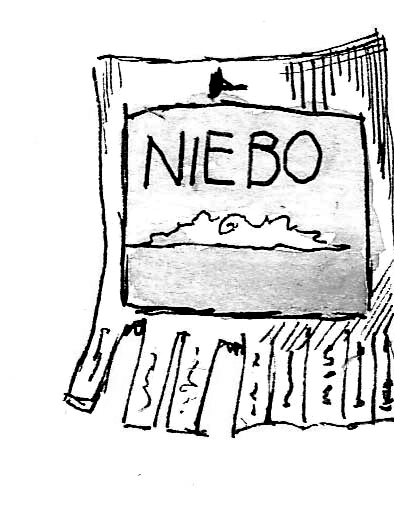
\includegraphics[height=3.6cm]{images/niebo.png}\vspace*{-3.65cm}\\
  \\
  \hspace*{5mm}Niebo do wynajęcia\\
  \hspace*{5mm}Niebo z widokiem na raj\\
  \hspace*{5mm}Tam gdzie spokój jest święty\\
  \hspace*{5mm}No i święci są pańscy\\
  \hspace*{5mm}Szklanką ciepłej herbaty\\
  \hspace*{5mm}Poczęstuje cię Pan\\
  \\
  Pomyślałem: to świetnie, takie niebo na ziemi\\
  Grzechów nikt nie przelicza, nikt nie szpera w szufladzie\\
  Pomyślałem: to świetnie, i spojrzałem na adres\\
  Lecz deszcz rozmył litery i już nie wiem gdzie jest\\
  \\
  Gdy wróciłem do domu, gdzie się błękit z betonem splata\\
  W Babel wysoki sięgający do chmur\\
  Zaparzyłem herbatę w swym pokoju nad światem\\
  Myśląc: nic nie straciłem, pewnie tak jest i tam\\
  \\
  \hspace*{5mm}W niebie do wynajęcia...\\
\end{minipage}
\begin{minipage}[t]{0.2\textwidth}
  a\\
  a\\
  d\\
  a\\

  G d a\\~\\~\\~\\~\\~\\

  a\\
  a\\
  d\\
  a\\

  a\\
  a\\
  d\\
  a\\
\end{minipage}

\newpage
\section{Niech żyje bal}\textcolor{lightgray}{\textit{Maryla Rodowicz}}\\~\\
\begin{minipage}[t]{0.8\textwidth}
  Życie, kochanie, trwa tyle, co taniec\\
  Fandango, bolero, be-bop\\
  Manna, hosanna, różaniec i szaniec\\
  I jazda i basta i stop\\
  Bal to najdłuższy na jaki nas proszą\\
  Nie grają na bis, chociaż żal\\
  Zanim więc serca upadłość ogłoszą\\
  Na bal, marsz na bal\\
  \\
  Szalejcie aorty, ja idę na korty\\
  Roboto, ty w rękach się pal\\
  Miasta nieczułe mijajcie jak porty\\
  Bo życie, bo życie to bal\\
  Bufet jak bufet zaopatrzony\\
  Zależy, czy tu, czy gdzieś tam\\
  Tańcz, póki żyjesz i śmiej się do żony\\
  I pij zdrowie dam\\
  \\
  \hspace*{5mm}Niech żyje bal! Bo to życie to bal jest nad bale\\
  \hspace*{5mm}Niech żyje bal! Drugi raz nie zaproszą nas wcale\\
  \hspace*{5mm}Orkiestra gra! Jeszcze tańczą i drzwi są otwarte\\
  \hspace*{5mm}Dzień wart jest dnia! A to życie zachodu jest warte\\
  \\
  Chłopo-robotnik jak boa grzechotnik\\
  Z niebytu wynurza się fal\\
  Wiedzie swa mamę i tatę i żonkę\\
  I rusza, wyrusza na bal\\
  Sucha kostucha - ta Miss Wykidajło\\
  Wyłączy nam prąd w środku dnia\\
  Pchajmy wiec taczki obłędu, jak Byron\\
  Bo raz mamy bal\\
\end{minipage}
\begin{minipage}[t]{0.2\textwidth}
  e\\
  H\\
  H$^7$\\
  e\\
  G\\
  D\\
  C\\
  H$^7$\\

  e\\
  H\\
  H$^7$\\
  e\\
  G\\
  D\\
  C\\
  H$^7$\\

  e H\\
  H$^7$ e\\
  e H\\
  H$^7$ e\\

  e\\
  H\\
  H$^7$\\
  e\\
  G\\
  D\\
  C\\
  H$^7$\\
\end{minipage}

\newpage
\section{Niewiele ci mogę dać}\textcolor{lightgray}{\textit{Perfect}}\\~\\
\begin{minipage}[t]{0.7\textwidth}
  Sto gorących słów gdy na dworze mróz\\
  W niewyspaną noc jeden koc\\
  Solo moich ust gitarowy blues\\
  Kilka dróg na skrót parę stów\\

  \hspace*{5mm}Nie mogę Ci wiele dać\\
  \hspace*{5mm}Nie mogę Ci wiele dać\\
  \hspace*{5mm}Bo sam niewiele mam\\
  \hspace*{5mm}Nie mogę dać wiele Ci\\
  \hspace*{5mm}Nie mogę dać wiele Ci\\
  \hspace*{5mm}Przykro mi\\

  Osiem znanych nut McCartneya but\\
  Kilka niezłych płyt jeden kicz\\
  Siedem chudych lat talię zgranych kart\\
  Południowy głód kurz i brud\\

  \hspace*{5mm}Nie mogę Ci wiele dać... $\times 2$\\

  Nadgryziony wdzięk pustej szklanki brzęk\\
  Niespełniony sen itp\\
  Podzielony świat myśli warte krat\\
  Zaleczony lęk weź co chcesz\\
\end{minipage}
\begin{minipage}[t]{0.3\textwidth}
  C a a$^7$\\
  d d$^7$ C (FC)\\
  C a a$^7$\\
  d d$^7$ C (BCF)\\

  F\\
  F$^{add9}$ G\\
  C ... BCBC\\
  F\\
  F$^{add9}$ G\\
  C ... (F C, C)\\

  C a a$^7$\\
  d d$^7$ C (FC)\\
  C a a$^7$\\
  d d$^7$ C (BCF)\\

  ~\\

  C a a$^7$\\
  d d$^7$ C (FC)\\
  C a a$^7$\\
  d d$^7$ C (BCF)\\
  \hspace*{-0.4cm} \vspace*{-1.4cm}
  \chord{t}{x,x,p3,p2,p1,p3}{{\small F$^{add9}$}}
\end{minipage}

\newpage
\section{Ona}\textcolor{lightgray}{\textit{Krzysztof Radzimski}}\\~\\
\begin{minipage}[t]{0.8\textwidth}
  Gdy ujrzała go, był maj, pachniały bzy\\
  W twarz uderzył wiatr, stanęły w oczach łzy\\
  On uśmiechnął się, podniósł dłoń, spojrzeniem przywołał ją\\
  Do siebie, ujęła jego dłoń, ścisnęła mocno\\
  Gdzieś w oddali ptak wzniósł pieśń radosną\\
  Czy to wiosny czar, czy miłosny żar sprawiły to\\
  \\
  \hspace*{5mm}Że ona robi loda mu, bo umi\\
  \hspace*{5mm}Robi loda mu, bo lubi to on\\
  \hspace*{5mm}Robi loda mu, jakie to piękne jest\\
  \hspace*{5mm}Że ona robi loda mu, bo umi\\
  \hspace*{5mm}Robi loda mu, bo lubi to on\\
  \hspace*{5mm}Robi loda mu, a wokół kwitną bzy\\

  Ciepłem swoich warg ogrzała go całego\\
  On palce w jej włosy wplótł i spojrzał w niebo\\
  W welurze jego ud znalazła schronienie swe\\
  I radość - przed końcem drogi tej nie czuł już lęku wcale\\
  Cytować zaczął więc Goethego w oryginale\\
  Po chwili białym bzem udekorował włosy jej\\

\end{minipage}
\begin{minipage}[t]{0.2\textwidth}
  a\\
  G\\
  F E\\
\end{minipage}

\newpage
\section{Opadły mgły}\textcolor{lightgray}{\textit{SDM}}\\~\\
\begin{minipage}[t]{0.7\textwidth}
  Opadły mgły i miasto ze snu się budzi\\
  Górą czmycha już noc\\
  Ktoś tam cicho czeka, by ktoś powrócił\\
  Do gwiazd jest bliżej niż krok\\
  Pies się włóczy popod murami bezdomny\\
  Niesie się tęsknota czyjaś na świata cztery strony\\

  A ziemia toczy, toczy swój garb uroczy\\
  Toczy, toczy się los
  \hspace*{5mm} $\times $2\\

  Ty, co płaczesz, ażeby śmiać mógł się ktoś\\
  Już dość! Już dość! Już dość!\\
  Odpędź czarne myśli, dość już twoich łez\\
  Niech to wszystko przepadnie we mgle\\

  Bo nowy dzień wstaje, bo nowy dzień wstaje\\
  Nowy dzień \hspace*{16mm} $\times $2\\
  Wstaje nowy dzień\\

  Z dusznego snu już miasto się wynurza\\
  Słońce wschodzi gdzieś tam\\
  Tramwaj na przystanku zakwitł jak róża\\
  Uchodzą cienie do bram\\
  Ciągną swoje wózki dwukółki mleczarze\\
  Nad dachami snują się sny podlotków pełne marzeń\\

  A ziemia toczy, toczy swój garb uroczy\\
  Toczy, toczy się los
  \hspace*{5mm} $\times $2\\

  Ty, co płaczesz, ażeby śmiać mógł się ktoś\\
  Już dość! Już dość! Już dość!\\
  Odpędź czarne myśli, porzuć błędny wzrok\\
  Niech to wszystko zabierze już noc\\

  Bo nowy dzień wstaje, bo nowy dzień wstaje\\
  Nowy dzień \hspace*{15mm} $\times $2\\
  Wstaje nowy dzień\\
\end{minipage}
\begin{minipage}[t]{0.3\textwidth}
  C F\\
  C G\\
  C F\\
  C G\\
  C F\\
  C G\\ C\\
  C F\\
  C G\\

  C F\\
  C G\\
  C F\\
  C G\\

  C F\\
  C G\\
  C\\

  C F\\
  C G\\
  C F\\
  C G\\
  C F\\
  C G\\
  C\\
  C F\\
  C G\\

  C F\\
  C G\\
  C F\\
  C G\\

  C F\\
  C G\\
  C\\

\end{minipage}

\newpage
\section{Oprócz błękitnego nieba}\textcolor{lightgray}{\textit{Marek Jackowski}}\\~\\
\begin{minipage}[t]{0.8\textwidth}
  Kiedy jestem sam\\
  Przyjaciele są daleko, daleko, ode mnie, ode mnie\\
  (...)~\\
  Gdy mam wreszcie czas dla siebie\\

  Wtedy sobie wspominam\\
  Dawne, dobre czasy\\
  Czuję się jakoś dziwnie\\
  Dzisiaj noc jest czarniejsza\\

  \hspace*{5mm}Oprócz błękitnego nieba\\
  \hspace*{5mm}Nic mi dzisiaj nie potrzeba\\

  Gdzie są wszystkie dziewczęta\\
  Które kiedyś tak bardzo, tak bardzo kochałem, kochałem\\
  Kto z przyjaciół pamięta\\
  Ile razy dla nich przegrałem?\\

  W gardle zaschło mi\\
  I butelka zupełnie, zupełnie, już pusta, już pusta\\
  (...)\\
  Nikt do drzwi już dzisiaj nie zastuka\\

  \hspace*{5mm}Oprócz błękitnego nieba...\\

  \hspace*{5mm}Oprócz drogi szerokiej, oprócz góry wysokiej\\
  \hspace*{5mm}Oprócz kawałka chleba, oprócz błękitu nieba\\
  \hspace*{5mm}Oprócz błękitnego nieba\\
  \hspace*{5mm}Nic mi dzisiaj nie potrzeba\\

\end{minipage}
\begin{minipage}[t]{0.2\textwidth}
  d C\\
  A$^7$ B C\\
  (A$^7$)\\
  A$^7$ d\\

  d C\\
  A$^7$ B C\\
  A$^7$\\
  A$^7$ d\\

  B C d\\
  B C d\\

  d C\\
  A$^7$ B C\\
  A$^7$\\
  A$^7$ d\\

  d C\\
  A$^7$ B C\\
  (A$^7$)\\
  A$^7$ d\\

  ~\\~\\
  B C d\\
  B C d\\
  B C d\\
  B C d\\
\end{minipage}

\newpage
\section{Orawa}\textcolor{lightgray}{\textit{Andrzej Wierzbicki}}\\~\\
\begin{minipage}[t]{0.8\textwidth}
  Z mego okna widać chmury na skalistych grzędach\\
  Przetrę szybę ciepłą dłonią, razem z nimi siędę	\\
  I będą mi grały wiatry na organach turni\\
  Kiedy pójdę zbójnikować nad dachami równin		\\
  /Moje życie tylko w górach, nad dachami równin/\\
  \\
  Z mego okna widać potok doliną, doliną\\
  Dumnych smreków las szeroki, mgły w kosodrzewinach\\
  I będą mi grały watry w zaklętych kolebach\\
  Noc krzesanym się zatańczy po niebach, po niebach\\
  \\
  \hspace*{5mm}Orawo, wiatrem malowany dach				\\
  \hspace*{5mm}Ciupagami wysrebrzony na smrekowych pniach\\
  \hspace*{5mm}Orawo, wiatrem malowany dom				\\
  \hspace*{5mm}Gdzie zbójnickie śpiewogrania po kolebach śpią\\

\end{minipage}
\begin{minipage}[t]{0.2\textwidth}
  a C d  E\\
  a C d E (E$^7$)\\
  F C d  E\\
  a C d E a\\
  \\
  \\
  a C d  E\\
  a C d E (E$^7$)\\
  F C d  E\\
  a C d E a\\
  \\
  F C d E\\
  C G H$^7$ E (E$^7$)\\
  F C d  E\\
  F E \\
\end{minipage}

\newpage
\section{Ośmiominutówka}\textcolor{lightgray}{\textit{}}\\~\\
\begin{minipage}[t]{0.82\textwidth}
  Mimozami jesień się zaczyna, złotawa, krucha i miła\\
  To ty, to ty jesteś ta dziewczyna, która do mnie na ulicę wychodziła\\
  \\
  Oh please, stand by me, Diana!\\
  \\
  Komu bliski bajek świat, kto u wróżek szuka rad\\
  Temu opowiedzieć chcę o wspaniałym moim śnie\\
  \\
  Pogasły ogniska w Hawiarskiej Kolibie\\
  Do snu kładzie się cała izba\\
  \\
  Już teraz wiem, że dni są tylko po to\\
  By do ciebie wracać każdą nocą złotą\\
  Nie znam słów, co mają jakiś większy sens\\
  Jeśli tylko jedno, jedno tylko wiem\\
  Być tam, zawsze tam, gdzie ty\\
  \\
  O, Majka, nie jestem ciebie wart\\
  O, Majka, zmieniłbym dla ciebie cały świat\\
  \\
  Dziewczyno, dziewczyno, zamień słotę na lato\\
  Widziałem na ulicy, jak szłaś, szłaś z innym\\
  \\
  Jeśli zobaczę cię z tym żołnierzem\\
  Naszej miłości nic nie ocali\\
  \\
  Nie płacz, kiedy odjadę\\
  Sercem będę przy tobie\\
  Więc nie płacz, kiedy odjadę\\
  Zostawię ci tę melodię\\
  \\
  Odpowie ci wiatr wiejący przez świat\\
  Odpowie ci bracie tylko\\
  \\
  Anna Maria smutną ma twarz\\
  Anna Maria wciąż patrzy w dal\\
  \\
  Więc bardzo proszę, wejdź, tu siadaj, rozgość się\\
  I zdradź mi, kim tyś jest, Madame\\

\end{minipage}
\begin{minipage}[t]{0.18\textwidth}
  C a F G $/\times$2\\
  C a F G $/\times$2\\

  C a F G\\

  C a F G\\
  C a F G\\

  F G C a\\
  F G C a\\

  F G\\
  C a\\
  F G\\
  C a\\
  F G\\

  C a F G $/\times$2\\
  C a F G\\

  C a F G\\
  C a F G\\

  F G\\
  C a\\

  C a \\
  F G C a\\
  F G C a\\
  F G \\

  F G C a\\
  F G\\

  C a F G\\
  C a F G\\

  F G C a\\
  F G\\
\end{minipage}

\newpage
\begin{minipage}[t]{0.8\textwidth}
  {\large KRYSTYNA CZYCZA!}\\

  Zadzwoniłem do dziewczyny, rozmawiałem dwie godziny\\
  A ona powiedziała, że od dawna już nie kocha mnie\\
  Ej, dziewczyno niedobra, serce masz jak wąż kobra\\
  Och, jak bardzo jest mi źle, chyba włosy wyrwę se\\
  Ej, dziewczyno moja zła, serce chyba masz ze szkła\\
  Cóżeś mi uczyniła, włosów mnie pozbawiła\\
  Ej, dziewczyno dość głupia, nie chcesz pójść w me ramiona\\
  Me ramiona fajne są, wszystkie dziewczyny to wią\\

  Loly pop, loly pop, u loly loly pop\\

  Always look on the bright side of life\\
  {\small \textit{(impro)}}\\
  (…Nobody expects the Spanish Inquisition!)\\

  So, always look on the bright side of death\\
  Just before you draw your terminal breath\\
  \\
  Pieski małe dwa chciały przejść przez rzeczkę\\
  Nie wiedziały jak, znalazły kładeczkę\\
  Kładka była zła, skąpały się pieski dwa\\
  Sibon sibon sia la la la la\\
  \\
  Pieski małe dwa poszły więc na łączkę\\
  Zobaczyły tam odrąbaną rączkę\\
  No a rączka ta sześć małych paluszków ma\\
  Sibon sibon sia la la la la\\

  {\small \textit{(solo)}}

\end{minipage}
\begin{minipage}[t]{0.2\textwidth}
  C a F G\\

  F G C a\\
  F G C a\\
  F G C a\\
  F G C a\\
  F G C a\\
  F G C a\\
  F G C a\\
  F G C a\\

  C a F G\\

  C a F G\\
  \\
  \\
  \\
  C a F G\\
  C a F G\\

  C a F G\\
  C a F G\\
  C a F G\\
  C a F G\\

  C a F G\\
  C a F G\\
  C a F G\\
  C a F G\\

\end{minipage}

% \newpage
% \section{Parostatek}\textcolor{lightgray}{\textit{Krzysztof Krawczyk}}\\~\\
% \begin{minipage}[t]{0.8\textwidth}
% W starym albumie u mego dziadka\\
% Jest takie zdjęcie, istny cud\\
% Płynacy w falach, wsród mewek stadka\\
% Statek na parę sprzed lat stu\\

% Tłum marynarzy pokład mu zdobi\\
% Słonce na górze pięknie lśni\\
% Dobry fotograf to zdjecie zrobił\\
% Wszystko jak żywe, aż się cni\\

% \hspace*{5mm}Parostatkiem w piękny rejs, statkiem na parę w piękny rejs\\
% \hspace*{5mm}Przy wtórze klątw bosmana, głośnych krzyków aż od rana\\
% \hspace*{5mm}Tak śpiewnie dusza łka\\

% \hspace*{5mm}Kąpielowy kostium włóż i na pokładzie ciało złóż\\
% \hspace*{5mm}Bo tutaj szum maszyny, bo tutaj głosem dziewczyny\\
% \hspace*{5mm}Tak cudnie sruba gra\\

% Dziadek bosmanem był na tym statku\\
% Wsród majtków wzbudzał wiecznie strach\\
% Krzyczał, aż drżały na brzegach kwiatki\\
% Cała załoga stała we łzach\\

% Lecz kiedy dziadek fajkę zapalił\\
% Tytoń mu zaczął płuca grzać\\
% Dziadek coś nucił, tytoń się palił\\
% Marzył, by wieki mogł tam trwać\\

% \hspace*{5mm}Parostatkiem w piękny rejs...\\

% \hspace*{5mm}La la la la la la la...\\
% \end{minipage}
% \begin{minipage}[t]{0.2\textwidth}
% \textcolor{red}{TODO}\\
% \end{minipage}

\newpage
\section{Pejzaże harasymowiczowskie}\textcolor{lightgray}{\textit{WGB}}\\~\\
\begin{minipage}[t]{0.8\textwidth}
  Kiedy stałem w przedświcie, a Synaj\\
  Prawdę głosił przez trąby wiatru\\
  Zasmreczyły się chmury igliwiem\\
  Bure świerki o góry wsparte\\
  I na niebie byłem ja jeden\\
  Plotąc pieśni w warkocze bukowe\\
  I schodziłem na ziemię za kwestą\\
  Przez skrzydlącą się bramę Lackowej\\
  \\
  \hspace*{5mm}I był Beskid i były słowa\\
  \hspace*{5mm}Zanurzone po pępki w cerkwi baniach\\
  \hspace*{5mm}Rozłożyście złotych\\
  \hspace*{5mm}Smagających się wiatrem do krwi\\
  \\
  Moje myśli biegały końmi\\
  Po niebieskich, mokrych połoninach\\
  I modliłem się, złożywszy dłonie\\
  Do gór, do Madonny brunatnolicej\\
  A gdy serce kroplami tęsknoty\\
  Jęło spadać na góry sine\\
  Czarodziejskim kwiatem paproci\\
  Rozgwieździła się Bukowina\\
\end{minipage}
\begin{minipage}[t]{0.2\textwidth}
  G D \\
  C e \\
  G D \\
  e C D\\
  G D \\
  C e \\
  G D \\
  e C D\\

  G  C G\\
  G C D\\
  D \\
  C D G\\

  G  D \\
  C e G\\
  G D \\
  e C D\\
  G D \\
  C e \\
  G D \\
  e C D\\
\end{minipage}

\newpage
\section{Piechotą do lata}\textcolor{lightgray}{\textit{Bajm}}\\~\\
\begin{minipage}[t]{0.7\textwidth}
  Znów przyjdzie maj, a z majem bzy\\
  I czekać mam na lepsze dni\\
  Znów przyjdzie mi nosić przykrótkie sny\\

  \hspace*{6mm}Do lata, do lata, do lata\\
  \hspace*{6mm}Piechotą będę szła\\
  \\
  \\
  Znów kupisz mi coś na imieniny\\
  Hmm, ja to wiem i czuję, że\\
  Znów przyjdzie mi nosić przykrótkie sny\\
  \\
  \\
  \hspace*{2mm}Przykrótkie sny nie w porę, zbyt lekko się ubiorę\\
  \hspace*{2mm}Noc długa świt w szronach i wiosna spóźniona\\
  \hspace*{2mm}I Twoje słowa zimne, że nie ma drogi innej\\
  \hspace*{2mm}Do lata, do lata, do lata tak dłuży się czas\\
  \hspace*{2mm}(Gdybyś tylko chciał)\\
  \\
  To byłoby to lato już\\
  I słońce, i szaleństwo burz\\
  Lecz dajesz mi tylko przykrótkie sny\\
\end{minipage}
\begin{minipage}[t]{0.3\textwidth}
  C a d$^7$ G$^7$\\
  C a d$^7$ G$^7$\\
  C E$^7$ a D$^7$\\

  C a d$^7$\\
  G$^7$ C\\
  \\
  (a d$^7$ G)\\
  C a d$^7$ G$^7$\\
  C a d$^7$ G$^7$\\
  C E$^7$ a D$^7$\\

  (F C C$^7$)\\
  F Gis\\
  C C$^7$\\
  D$^7$\\
  G Gis G\\
  \\
  \\
  C a d$^7$ G$^7$\\
  C a d$^7$ G$^7$\\
  C E$^7$ a D$^7$\\

\end{minipage}

\newpage
\section{Pieśń o przyjacielu}\textcolor{lightgray}{\textit{Włodzimierz Wysocki}}\\~\\
\begin{minipage}[t]{0.5\textwidth}
  ~\\
  Gdy w twym życiu się zjawił ktoś\\
  Kto wygląda jak równy gość\\
  Ale nie wiesz, czy szczery jest\\
  Czy na pokaz ma gest\\
  \hspace*{5mm}Weź go w góry na stromy stok\\
  \hspace*{5mm}Nie odstępuj go tam na krok\\
  \hspace*{5mm}Jedna lina niech łączy was\\
  \hspace*{5mm}Dla was dwóch to w sam raz\\
  \\
  Jeśli w górach się bał i drżał\\
  Jeśli zmiękł i się pluł - chcę w dół\\
  A gdy dłoń skaleczoną miał\\
  Wniebogłosy się darł\\
  \hspace*{5mm}Lepiej pogoń go precz raz-dwa\\
  \hspace*{5mm}Nie na wiele się taki zda\\
  \hspace*{5mm}Taki w biedzie zawiedzie też\\
  \hspace*{5mm}I nie o nim ta pieśń\\
  \\
  Jeśli druh twój przez całe dnie\\
  Ani razu nie skarżył się\\
  A gdy spadłeś, to właśnie on\\
  Zaraz podał ci dłoń\\
  \hspace*{5mm}Jeśli dzielnie przy tobie trwał\\
  \hspace*{5mm}Jak do boju na szczyt się rwał\\
  \hspace*{5mm}Wiedz, że odtąd przez cały czas\\
  \hspace*{5mm}Przyjaciela w nim masz\\
\end{minipage}
\begin{minipage}[t]{0.5\textwidth}
  (a)\\
  E\\
  E$^7$ a\\
  A d\\
  d E\\
  d\\
  a\\
  E\\
  a\\

  E\\
  E$^7$ a\\
  A d\\
  d E\\
  d\\
  a\\
  E\\
  a\\

  E\\
  E$^7$ a\\
  A d\\
  d E\\
  d\\
  a\\
  E\\
  a\\
\end{minipage}

\newpage
\section{Piła}\textcolor{lightgray}{\textit{Zioma}}\\~\\
\begin{minipage}[t]{0.85\textwidth}
  Piła ucięła chuja wuja (ho hohoho)\\
  Drze wuju ryja, ała, ała (ho hohoho)\\
  \\
  \hspace*{3mm}Piła ucięła chuja wuja, o, piła ucięła chuja wuja, o\\
  \hspace*{3mm}Chuja wuja, o, chuja wuja, o, chuja wuja a-a…\\
  \hspace*{3mm}Lecz\\
  \\
  \hspace*{6mm}Jaja ma, łołoło jaja ma, łołoło jaja ma, łołoło jaja ma\\
  \hspace*{6mm}Łołoło jaja ma, łołoło jaja ma, łołoło jaja ma, łołoło\\

  I wije się wujek po trawniku (ho hohoho)\\
  Posoka sika, siku-siku (ho hohoho)\\
  \\
  I kumple mu mówią, widząc ptaka (ho hohoho)\\
  E, to nie taka wielka strata (ho hohoho)\\

  A wuj se z tego nie robi nic (ho hohoho)\\
  Zrywa się na równe nogi i (ho hohoho)\\

  \hspace*{3mm}I krzyczy wolność, hura hura, i krzyczy wolność, hura hura\\
  \hspace*{3mm}Hura hura, hura hura, hura a-a…\\

  \hspace*{6mm}Żegnajcie, łołoło żegnajcie, łołoło żegnajcie, łołoło żegnajcie \\
  \hspace*{6mm}Żegnajcie, kwiatki, bombonierki i tym podobne duperele\\
  \hspace*{6mm}Upominki, Walentynki i kwaśne minki z powodu złamanej szminki\\
  \hspace*{6mm}I żegnaj wreszcie i ty, niezgodności nauki kościoła katolickiego\\
  \hspace*{6mm}Z naturalną potrzebą człowieka do używania lateksu profilakcyjnego\\
  \hspace*{6mm}Fridom!\\
\end{minipage}
\begin{minipage}[t]{0.2\textwidth}
  C G F C\\
  C G F C\\

  a A$^{sus2}$ $/ \times$4\\
  (G)\\
  G$^7$\\

  C F C G C\\
  C F C G C\\

  C G F C\\
  C G F C\\

  C G F C\\
  C G F C\\

  C G F C\\
  C G F C\\

  a A$^{sus2}$ $/ \times$4\\
  G G$^7$\\

  C F C G C\\
\end{minipage}
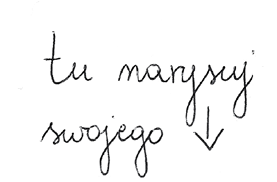
\includegraphics[width=0.15\textwidth, center]{images/pila.png}\\

\newpage
\section{Piosenka kontrowersyjna}\textcolor{lightgray}{\textit{Zioma}}\\
\begin{minipage}[t]{0.8\textwidth}
  ~\\
  \hspace*{6.5cm}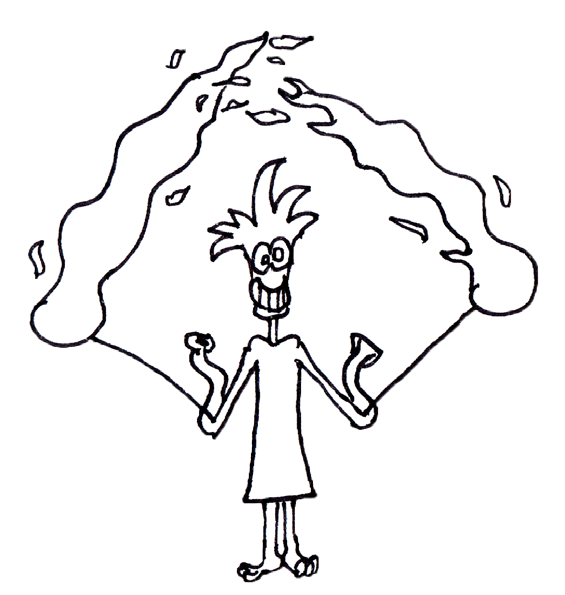
\includegraphics[height=3.9cm,left]{images/piosenka_kontrowersyjna.png}\vspace*{-3.91cm}\\
  Matka ateistka							\\
  Teściowa wierzy w Boga\\
  \\
  \hspace*{4mm}Jestem pojebany, jestem pojebany\\
  \hspace*{4mm}Z tej prostej przyczyny\\
  \hspace*{8mm}Że wierzę w dziewczyny\\
  \hspace*{8mm}Że kocham dziewczyny\\
  \hspace*{8mm}Że się biją dziewczyny\\
  \\
  A teraz pozdrowienia dla dziewczyn z całego świata przesyłam z miasta\\
  Łodzi, bo stąd fala się rozchodzi!\\
  \\
  Jestem pojebany, jestem pojebany				\\
  Muszę iść do mamy, idę już do mamy\\
\end{minipage}
\begin{minipage}[t]{0.2\textwidth}
  ~\\
  C a F G\\
\end{minipage}

% \newpage
\section{Piosenka wiosenna}\textcolor{lightgray}{\textit{WGB}}\\~\\
\begin{minipage}[t]{0.8\textwidth}
  ~\\~\\
  Zagram dla ciebie na każdej gitarze świata\\
  Na ulic fletach, na nitkach babiego lata\\
  Wyśpiewam, jak potrafię, księżyce na rozstajach\\
  I wrześnie, i stycznie, i maje\\
  I zagubione dźwięki i barwy na płótnach Vlamincka\\
  I słońce wędrujące promienia ścieżynką\\
  \\
  \hspace*{5mm}Graj nam, graj, pieśni skrzydlata\\
  \hspace*{5mm}Wiosna taniec nasz niesie po łąkach\\
  \hspace*{5mm}Zatańczymy się w sobie do lata\\
  \hspace*{5mm}Zatańczymy się w siebie bez końca\\
  \\
  A blask, co oświetla me ręce, gdy piszę\\
  Nabrzmiał potrzebą rozerwania ciszy\\
  Przez okno wyciekł, pełna go teraz chmara wronia\\
  Dziobie się w dziobów końcach, a w ogonach ogoni\\
  A pieśń moja to niknie, to wraca\\
  I nie wiem, co bym zrobił, gdybym ją utracił\\
\end{minipage}
\begin{minipage}[t]{0.2\textwidth}
  (C G F C $/ \times $2)\\(e)\\
  a e F G\\
  a e F G\\
  C G C F\\
  e F d G\\
  e e d G\\
  e F d G\\

  C G F C\\
  e F d G\\
  C F C G F\\
  C G F G C\\

  a e F G\\
  a e F G\\
  C G C F\\
  e F d G\\
  e e d G\\
  e F d G\\

\end{minipage}

% \newpage
% \section{Płachta nieba}\textcolor{lightgray}{\textit{Jacek Kleyff / Kwiat Jabłoni}}\\~\\
% \begin{minipage}[t]{0.8\textwidth}
% \hspace*{5mm}Rozpostarta płachta nieba\\
% \hspace*{5mm}Zawsze daje to, co trzeba\\
% \hspace*{5mm}Przez tę płachtę, pod sam kręgosłup\\
% \hspace*{5mm}Prześwituje sama wiedza\\
% \hspace*{5mm}Kiedy zbieram z niej bez wahań\\
% \hspace*{5mm}Zwykle trafiam w to, co czuję\\
% \hspace*{5mm}Jeśli mniej premedytuję\\
% \hspace*{5mm}Jeśli mniej kalkuluję\\

% Nie muszę tu być; Lecz cieszę się\\
% Gdy czasem jestem; Gdy czasem jestem\\
% Chociaż nie muszę stąd iść (póki co); Też cieszę się\\
% Gdy coś potrafię; Coś potrafię\\
% Kiedy nie muszę nic - potrafię musieć; Żyć na jawie\\
% Żyć na jawie; I uczyć się kochać\\

% \hspace*{5mm}Tę płachtę nieba...\\

% \hspace*{10mm}W przymusie żyć\\
% \hspace*{10mm}To być skazanym\\
% \hspace*{10mm}Na marzenia\\

% Gdy zmuszam kogoś do czegoś; To chyba właśnie chcę\\
% Przed własnym lękiem uciec; Ale gdzie?\\
% Ale gdzie tu zwiewać; No gdzie?\\
% Na tym świecie; I w tym ciele\\

% \hspace*{5mm}Rozpostarta płachta nieba... \hspace{5mm}$/\times$2\\

% Gdy muszę kpić; To chyba znak\\
% Że na to z czego kpię; Sił już nie mam\\
% Sił mi brak; Ja chyba muszę\\
% Nie musieć nic; I wtedy wiem\\
% Co naprawdę muszę; A czego nie\\
% \end{minipage}
% \begin{minipage}[t]{0.2\textwidth}
%   d \\
%   C \\
%   g \\
%   d C\\
%   d \\
%   C \\
%   g \\
%   d C\\

%   d C \\
%   g dC\\
%   d C \\
%   g dC\\
%   d C \\
%   g dC\\

%  % d d C C g g d C

% \textcolor{red}{TODO}\\
% \end{minipage}

\newpage
\section{Pocztówka z Beskidu}\textcolor{lightgray}{\textit{Wołosatki}}\\~\\
\begin{minipage}[t]{0.8\textwidth}
  Po Beskidzie błądzi jesień, wypłakuje deszczu łzy\\
  Na zgarbionych plecach niesie worek siwej mgły\\
  Pastelowe cienie kładzie, zdobiąc rozczochrany las\\
  Nocą rwie w brzemiennym sadzie grona słodkich gwiazd\\
  Złotych gwiazd\\
  \\
  \hspace*{5mm}Jesienią góry są najszczersze\\
  \hspace*{5mm}Żurawim kluczem otwierają drzwi\\
  \hspace*{5mm}Jesienią smutne piszę wiersze\\
  \hspace*{5mm}Smutne piosenki śpiewam ci\\
  \\
  Po Beskidzie błądzą ludzie, kare konie w chmurach rżą\\
  Święci pańscy zamiast w niebie po kapliczkach śpią\\
  Kowal w kuźni klepie biedę, czarci wydeptują trakt\\
  W pustej cerkwi, co niedzielę, rzewnie śpiewa wiatr\\
  Pobożny wiatr\\
  \\
  \hspace*{5mm}W Beskidzie zostawiłem serce\\
  \hspace*{5mm}Tu każde pasmo ma swój własny styl\\
  \hspace*{5mm}Tu z wami chcę wędrować wiecznie\\
  \hspace*{5mm}Bez tego smutno będzie mi\\
\end{minipage}
\begin{minipage}[t]{0.2\textwidth}
  G D e h$^7$\\
  C G a$^7$ D\\
  G D e h$^7$\\
  C G a$^7$ D\\
  G G$^7$\\

  C D G C\\
  C D G G$^7$\\
  C D G C\\
  C D G\\

  G D e h$^7$\\
  C G a$^7$ D\\
  G D e h$^7$\\
  C G a$^7$ D\\
  G G$^7$\\

  C D G C\\
  C D G G$^7$\\
  C D G C\\
  C D G\\
\end{minipage}

\newpage
\section{Polej jabole}\textcolor{lightgray}{\textit{Zioma}}\\~\\
\begin{minipage}[t]{0.8\textwidth}
  Polej jabole, Borys, polewaj jabole\\
  Jadą za meliną gieroje morowe\\
  Aby nabyć wina owocowe\\
  \\
  Wsjie ubieżają, bo gieroje czadu dają\\
  Skrzynka bełta na zakrętach się kołysze\\
  Ale będzie ubaw, towarzysze\\
  \\
  Dziewuszki placzut, już gieroji nie zobaczą\\
  Skosili znak „Zakaz wjazdu” JEB maluchem\\
  I upili milicjantów uchem\\
\end{minipage}
\begin{minipage}[t]{0.2\textwidth}
  d a d a\\
  B A\\
  B A\\

  d a d a\\
  B A\\
  B A\\

  d a d a\\
  B A\\
  B A\\
\end{minipage}

% \newpage
\section{Połoniny niebieskie}\textcolor{lightgray}{\textit{Adam Drąg}}\\~\\
\begin{minipage}[t]{0.8\textwidth}
  Gdy nie zostanie po mnie nic\\
  Oprócz pożółkłych fotografii\\
  Błękitny mnie przywita świt\\
  W miejscu, co nie ma go na mapie\\
  \\
  A kiedy sypną na mnie piach\\
  Gdy mnie okują cztery deski\\
  To pójdę tam, gdzie wiedzie szlak\\
  Na połoniny, na niebieskie\\
  \\
  Powiedzie mnie błękitny wóz\\
  Ciągnięty przez błękitne konie\\
  Przez świat błękitny będzie wiózł\\
  Aż zaniebieszczy w dali błonie\\
  \\
  Od zmartwień wolny i od trosk\\
  Pójdę wygrzewać się na trawie\\
  A czasem, gdy mi przyjdzie chęć\\
  Z góry na ziemię się pogapię\\
  \\
  Popatrzę jak wśród smukłych malw\\
  Wiatr w przedwieczornej ciszy kona\\
  Trochę mi tylko będzie żal\\
  Że trawa u was tak zielona\\
\end{minipage}
\begin{minipage}[t]{0.2\textwidth}
  C F C F\\
  C F C G\\
  e F C G\\
  C F C F\\

  C F C F\\
  C F C G\\
  e F C G\\
  C F C F\\

  C F C F\\
  C F C G\\
  e F C G\\
  C F C F\\

  C F C F\\
  C F C G\\
  e F C G\\
  C F C F\\

  C F C F\\
  C F C G\\
  e F C G\\
  C F C F\\

\end{minipage}

\newpage
\section{Pożegnalny ton}\textcolor{lightgray}{\textit{Mechanicy Shanty}}\\~\\
\begin{minipage}[t]{0.75\textwidth}
  Chyba dobrze wiesz już, jaką z dróg\\
  Popłyniesz, kiedy serce rośnie ci nadzieją\\
  Że jeszcze są schowane gdzieś\\
  Nieznane lądy, które szczęście twe odmienią\\
  \\
  Chyba dobrze wiesz już, jaką z dróg\\
  Wśród białej fali piany statek twój popłynie\\
  A jeśli tak, spotkamy się\\
  Na jakiejś łajbie, którą szczęście swe odkryjesz\\

  \hspace*{5mm}Morza i Oceany grzmią\\
  \hspace*{5mm}Pieśni pożegnalny ton\\
  \hspace*{5mm}Jeszcze nieraz zobaczymy się\\
  \hspace*{5mm}A teraz czas stawiać żagle i z portu wyruszać nam w rejs\\
  \\
  W kolorowych światłach keja lśni\\
  A główki portu sennie mruczą: do widzenia\\
  A jutro, gdy nastanie świt\\
  W rejs wyruszymy, by odkrywać swe marzenia\\

  Nim ostatni akord wybrzmi już\\
  Na pustej scenie nieme staną mikrofony\\
  Ostatni raz śpiewamy dziś\\
  Na pożegnanie wszystkim morzem urzeczonym\\
\end{minipage}
\begin{minipage}[t]{0.25\textwidth}
  D fis\\
  e G A\\
  G Fis$^7$ h G\\
  D G A D\\
  \\
  D fis\\
  e G A\\
  G Fis$^7$ h G\\
  D G A D\\
  \\
  D A h G\\
  D G A D\\
  D A h G\\
  D A D\\
  \\
  D fis\\
  e G A\\
  G Fis$^7$ h G\\
  D G A D\\
  \\
  D fis\\
  e G A\\
  G Fis$^7$ h G\\
  D G A D\\
\end{minipage}

\newpage
\section{Pożegnanie gór}\textcolor{lightgray}{\textit{Ireneusz Lament}}\\~\\
\begin{minipage}[t]{0.8\textwidth}
  Słońca dysk zaginął już w konarach	\\
  Na polanę spłynął szary mrok		\\
  Smętnie zadzwoniła gdzieś gitara	\\
  W ciemnej ciszy czyjś zamiera krok	\\
  \\
  Przy ognisku wędrowców gromada\\
  W blasku iskier zamarł cieni krąg\\
  Wysłuchują struny opowiadań\\
  Zasłyszanych gdzieś daleko stąd\\
  \\
  Pięciolinią wyznaczonym szlakiem				\\
  Błądzi zapomniany, wieczny cień				\\
  A w swych troskach smętnie zadumany			\\
  Żegna świątek odchodzący dzień			\\
  \\
  Znika w dali kalejdoskop twarzy\\
  Zgasłych ognisk dym już sięga chmur\\
  Pomyśl, ile niespełnionych marzeń\\
  Łączy z sobą pożegnanie gór\\
  \\
  Już nie znikną góry z twoich wspomnień\\
  Oczy ikon, nieprzebyty szlak\\
  Szumu jodeł nie da się zapomnieć\\
  Będziesz do nich wracał w swoich snach\\
\end{minipage}
\begin{minipage}[t]{0.2\textwidth}
  a d a A$^7$\\
  d G C A$^7$\\
  d G C a\\
  d E a (A$^7$)\\

  a d a A$^7$\\
  d G C A$^7$\\
  d G C a\\
  d E a (A$^7$)\\

  a d a A$^7$\\
  d G C A$^7$\\
  d G C a\\
  d E a (A$^7$)\\

  a d a A$^7$\\
  d G C A$^7$\\
  d G C a\\
  d E a (A$^7$)\\

  a d a A$^7$\\
  d G C A$^7$\\
  d G C a\\
  d E a (A$^7$)\\
\end{minipage}

\newpage
\section{Pożegnanie z górami}\textcolor{lightgray}{\textit{Włodzimierz Wysocki}}\\~\\
\begin{minipage}[t]{0.8\textwidth}
  W rozgwar ogromnych miast, w światła ulic, mrok bram\\
  Powracamy, lecz tam też za mało nam miejsca\\
  Dziś zdobyliśmy szczyt, ale smutno jest nam\\
  Pozostały wśród gór, pozostały wśród gór\\
  Nasze serca\\
  \\
  \hspace*{3mm}Więc przestańcie już gadać o bzdurach\\
  \hspace*{3mm}Zrozumiałem i łatwiej mi żyć\\
  \hspace*{3mm}Piękniej niż w górach jest tylko w tych górach\\
  \hspace*{3mm}Gdzie nie byłem i gdzie muszę być\\
  \\
  Kto by chciał w chwili złej zostać naprawdę sam?\\
  Kto by szczęściu dał spać, jeśli obok tuż drzemie?\\
  Dziś zdobyliśmy szczyt, ale smutno jest nam\\
  Przecież nawet i Bóg, przecież nawet i Bóg\\
  Musiał zejść na tę ziemię\\
  \\
  Co ocalić się da z naszych szlaków i tras\\
  Czasem złoży się w wiersz lub piosenkę zanuci\\
  Dziś zdobyliśmy szczyt, może ostatni raz\\
  Lecz na pewno za rok, lecz na pewno za rok\\
  Ktoś tu znowu powróci\\
  \\
  \foreignlanguage{russian}{
    \hspace*{5mm} Так оставьте ненужные споры!\\
    \hspace*{5mm} Я себе уже всё доказал -\\
    \hspace*{5mm} Лучше гор могут быть только горы,\\
    \hspace*{5mm} На которых еще не бывал.\\
  }
\end{minipage}
\begin{minipage}[t]{0.2\textwidth}
  a\\
  A d\\
  d a\\
  E\\
  a\\

  a d \\
  d a \\
  A d \\
  d E / E a\\

  a\\
  A d\\
  d a\\
  E\\
  a\\

  a\\
  A d\\
  d a\\
  E\\
  a\\

  a d \\
  d a \\
  A d \\
  d E / E a\\

\end{minipage}

\newpage
\section{Praca}\textcolor{lightgray}{\textit{Zioma}}\\
\begin{minipage}[t]{0.8\textwidth}
  Na ni ni ni ni na ni na nej nej…\vspace*{1.6mm}

  Tato, co mam robić, pytam się swojego taty\\
  Tato na to: nie pracuj, bo będziesz garbaty\\
  Bo praca, bo praca jest gorsza od kaca\\
  Kwiat świata od życia ta praca odwraca\\
  \hspace*{5mm}Odpręż się\\
  \hspace*{5mm}Praca gorsza jest od kaca, hehehe\vspace*{1.6mm}

  No to co mam robić, pytam się swojego taty\\
  Tato na to: Synek, idź powąchać kwiaty\\
  Są też inne podniety, pety, kobiety\\
  Alkohole, przyjaciele, ele mele, jesteś cielę\\
  \hspace*{5mm}Odpręż się\\
  \hspace*{5mm}W zdrowym ciele zdrowe cielę, hehehe\vspace*{1.6mm}

  Ale tato, jak to sobie wyobrażasz szczegółowo\\
  Tato na to: Synek, musisz ruszyć głową\\
  Weź bandę od rozwałki i ruszaj na działki\\
  Zapal, nalej i zaszalej i pamiętaj, że\\
  \hspace*{5mm}Odpręż się\\
  \hspace*{5mm}Zapal, nalej i zaszalej, hehehe\vspace*{1.6mm}

  Dum da di di da dida dej…\vspace*{1.6mm}

  Tato, co ty na to, mówię do swojego taty\\
  Odpręzyłem się totalnie i jestem scerbaty\\
  Zapalałem i nalałem, nie wylałem nic za siebie\\
  Zobacyłem ją psy dzewie, pocułem się jak w niebie\\
  \hspace*{5mm}Odpręzyłem się\\
  \hspace*{5mm}I pocułem się jak w niebie, hehehe\vspace*{1.6mm}

  No i z rykiem, stolikiem, ktoś zaatakował mnie\\
  Usta zdejm z niej ty typie\\
  Moja to dziewoja, kawał gnoja jesteś ty\\
  Gwiazdy zabłysły i posły kły\\
  \hspace*{5mm}Posły kły\\
  \hspace*{5mm}Gwiazdy zabłysły i posły kły\vspace*{1.6mm}

  A morał, a morał w tym momencie dotyka\\
  Tego pana terrorystę od stolika\\
  Niepotrzebnie tak nerwowo uniósł się\\
  Chyba nikt mu nie powiedział w porę, że\\
  \hspace*{5mm}Odpręż się\\
  \hspace*{5mm}Nikt mu nie powiedział w porę\vspace*{1.6mm}

  \hspace*{3mm}Tyl Tyl tylko wycieczki\\
  \hspace*{3mm}Powodują, że nie mam cieczki\\
\end{minipage}
\begin{minipage}[t]{0.2\textwidth}
  a e G D\vspace*{2mm}

  a e\\
  G D\\
\end{minipage}

\newpage
\section{Preluduim dla Leonarda}\textcolor{lightgray}{\textit{Leonard Luther}}\\~\\
\begin{minipage}[t]{0.81\textwidth}
  Na parterze w mojej chacie mieszkał kiedyś taki facet\\
  Który dnia pewnego cicho do mnie rzekł\\
  Gdy zachwycisz się dziewczyną, nie podrywaj jej na kino\\
  Ale patrząc prosto w oczy, szepnij słowa te\\

  \hspace*{4mm}Jestem taki samotny, jak palec albo pies\\
  \hspace*{4mm}Kocham wiersze Stachury i stary dobry jazz\\
  \hspace*{4mm}Szczęścia w życiu nie miałem, rzucały mnie dziewczyny\\
  \hspace*{4mm}Szukam cichego portu, gdzie okręt mój zawinie\\

  Po tych słowach, z miłosierdzia, padła już niejedna twierdza\\
  I niejedna cnota chyżo poszła w las\\
  Ryba bierze na robaki, a panienka na tekst taki\\
  Który zawsze mówię, patrząc prosto w twarz\\

  Gdy szał pierwszych zrywów minął, zakochałem się w dziewczynie \\
  Z którą się na całe życie zostać chce\\
  Chciałem rzec: będziemy razem, zrozumiała mnie od razu\\
  I jak echo wyszeptała słowa te\\

  \hspace*{4mm}Jesteś taki samotny...\\

  \hspace*{4mm}Jestem taka samotna, jak palec albo miotła\\
  \hspace*{4mm}Kocham wiersze Leśmiana i szaleć aż do rana\\
  \hspace*{4mm}Szczęścia w życiu nie miałam, chłopaków olewałam\\
  \hspace*{4mm}Szukam cichego portu do uprawiania sportu\\
\end{minipage}
\begin{minipage}[t]{0.19\textwidth}
  D  G D\\
  C  G D\\
  C G D A\\
  C  G D\\

  h G D A\\
  C G D \\
  h G D A\\
  C G D \\

  D G D \\
  C G D \\
  C G D A\\
  C G D \\

  D G D \\
  C G D \\
  C G D A\\
  C G D \\

  ~\\~\\
  h G D A\\
  C G D \\
  h G D A\\
  C G D \\
\end{minipage}

\newpage
\section{Prosektorium}\textcolor{lightgray}{\textit{Piotr Narkiewicz}}\\~\\
\begin{minipage}[t]{0.75\textwidth}
  Leży na stole głowa, jaka piękna połowa\\
  Obok świeża i miękka leży jakaś ręka\\
  \\
  \hspace*{5mm}A ty stoisz i się temu przyglądasz\\
  \hspace*{5mm}Lecz uśmiechnij się, bo za chwilę czeka cię twoje ulubione\\
  \hspace*{5mm}Prosektorium\\
  \\
  \hspace*{7cm}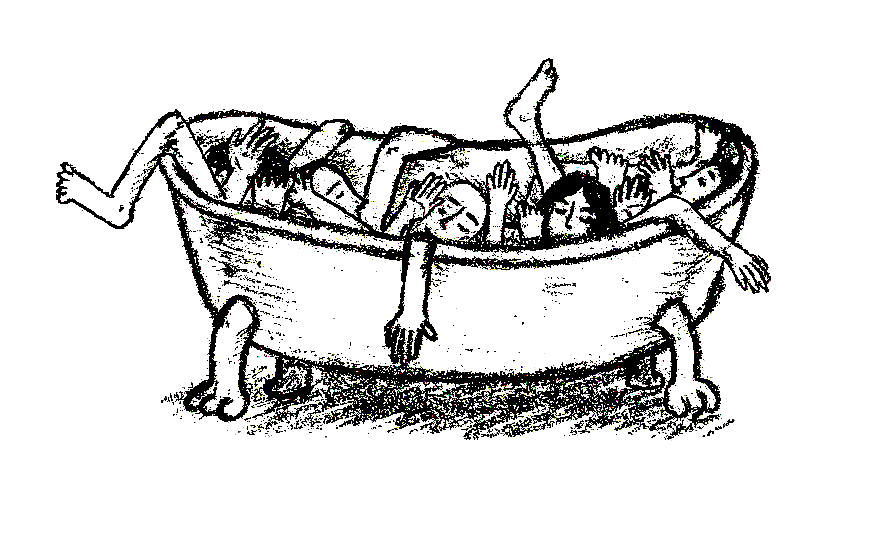
\includegraphics[height=3cm]{images/prosektorium.png}\vspace*{-3.05cm}\\
  Na półce, wysoko, patrzy jedno oko\\
  A w ciemnej głuszy nasłuchują uszy\\
  \\
  Pływają w wanience nogi, głowy i ręce\\
  Wszystko się kotłuje, zaraz zwymiotuję\\
  \\
  Można tutaj znaleźć każdą cząstkę ciała\\
  Tylko duszy nie ma, dusza uleciała\\
\end{minipage}
\begin{minipage}[t]{0.25\textwidth}
  C\\
  \\
  \\
  F C\\
  Gis B\\
  C\\
  \\
\end{minipage}

% \newpage
\section{Przeżyj to sam}\textcolor{lightgray}{\textit{Lombard}}\\~\\
\begin{minipage}[t]{0.75\textwidth}
  Na życie patrzysz bez emocji\\
  Na przekór czasom i ludziom wbrew\\
  Gdziekolwiek jesteś, w dzień czy w nocy\\
  Oczyma widza oglądasz grę\\
  Ktoś inny zmienia świat za ciebie\\
  Nadstawia głowę, podnosi krzyk\\
  A ty z daleka, bo tak lepiej\\
  I w razie czego nie tracisz nic\\

  \hspace*{5mm}Przeżyj to sam, przeżyj to sam\\
  \hspace*{5mm}Nie zamieniaj serca w twardy głaz\\
  \hspace*{5mm}Póki jeszcze serce masz\\

  Widziałeś wczoraj znów w dzienniku\\
  Zmęczonych ludzi wzburzony tłum\\
  I jeden szczegół wzrok twój przykuł\\
  Ogromne morze ludzkich głów\\
  A spiker cedził ostre słowa\\
  Od których nagła wzbierała złość\\
  I począł w tobie gniew kiełkować\\
  Aż pomyślałeś: milczenia dość\\
\end{minipage}
\begin{minipage}[t]{0.25\textwidth}
  C E$^7$ a\\
  d d$^7$ G G$^7$\\
  C E$^7$ a\\
  d d$^7$ G G$^7$\\C E$^7$ a\\
  d d$^7$ G G$^7$\\C E$^7$ a\\
  d d$^7$ G G$^7$\\

  C E a d d$^7$ G G$^7$\\
  C E$^7$ a\\
  d d$^7$ G G$^7$\\

  C E$^7$ a\\
  d d$^7$ G G$^7$\\
  C E$^7$ a\\
  d d$^7$ G G$^7$\\
  C E$^7$ a\\
  d d$^7$ G G$^7$\\
  C E$^7$ a\\
  d d$^7$ G G$^7$\\
\end{minipage}

\newpage
\section{Przyszedłem po to}\textcolor{lightgray}{\textit{Piotr Narkiewicz}}\\~\\
\begin{minipage}[t]{0.8\textwidth}
  Nie umiem mówić wielkich słów\\
  Więc ci nie powiem, po co tu przyszedłem\\
  Zgubiłem drogę albo padał deszcz\\
  Przechodziłem, więc wszedłem\\

  \hspace*{5mm}Przyszedłem po to, by uśmiechnąć się do ciebie\\

  Tyle rzeczy wydarzyło się\\
  Może zbyt wiele, lecz nie jestem przecież w biedzie\\
  Przyszedłem dzisiaj po to, by\\
  Zapytać, jak ci się wiedzie\\
  \\
  Sam dobrze nie wiem, po co tu przyszedłem\\
  Może po prostu chciałem cię zobaczyć\\
  Jak dziś wyglądasz i co robisz dziś wieczorem\\
  Jaki płaszcz ubierasz na spacer\\
  \\
  A może spytać, jak ci minął dzień\\
  Albo, jak kiedyś, trochę z drogi zboczyć\\
  By kolejny raz przekonać się\\
  Jakie masz śliczne, brązowe oczy\\
  \\
  Pytasz, co robię, przecież sama dobrze wiesz\\
  Pracuję, chodzę i znam trochę nowych osób\\
  Dzisiaj przyszedłem po to, by\\
  Po prostu posłuchać twojego głosu\\

  A może chciałem tylko przyjść\\
  Zobaczyć, co u ciebie słychać\\
  I móc posiedzieć u twych stóp\\
  \hspace*{1.4cm}\ldots I o nic już nie pytać\\
\end{minipage}
\begin{minipage}[t]{0.2\textwidth}
  a h E\\~\\~\\~\\~\\
  d E a\\

\end{minipage}

\newpage
\section{Rawhide}\textcolor{lightgray}{\textit{The Blues Brothers}}\\~\\
\begin{minipage}[t]{0.8\textwidth}
  ~\\
  \hspace*{5cm}
\includegraphics[height=1.5cm, angle=-10]{images/rawhide.png}\vspace*{-1.84cm}\\
  Rollin', rollin', rollin' /x4\\
  Rawhide\\
  \\
  \\
  Rollin', rollin', rollin', though the streams are swollen\\
  Keep them doggies rollin', rawhide\\
  Through rain an' wind an' weather, hell bent for leather\\
  Wishin' my gal was by my side\\
  All the things I'm missin', Good vittles, love an' kissin'\\
  Are waitin' at the end of my ride\\
  \\
  Move 'em on (head 'em up), head 'em up (move 'em on) \\
  Move 'em on (head 'em up), rawhide\\
  Cut 'em out (ride 'em in), ride 'em in (cut 'em out)\\
  Cut 'em out, ride 'em in, rawhide\\

  Keep movin', movin', movin', though they're disapprovin'\\
  Keep them doggies movin', rawhide\\
  Don't try to understand 'em, just rope, throw an' brand 'em\\
  Soon we'll be livin' high an' wide\\
  My heart's calculatin', my true love will be waitin'\\
  Be waitin' at the end of my ride\\
\end{minipage}
\begin{minipage}[t]{0.2\textwidth}
  ~\\
  a\\
  \\
  \\
  \\
  a C\\
  E\\
  a G a\\
  G F E E$^7$\\
  a G a\\
  G a G a\\
  \\
  a E \\
  a E \\
  a E\\
  a F E a\\

  a C\\
  E\\
  a G a\\
  G F E E$^7$\\
  a G a\\
  G a G a\\
\end{minipage}

\includegraphics[width=0.5\textwidth,angle=-30, center]{images/rawhide.png}\\

\newpage
\section{Róża Czerwono}\textcolor{lightgray}{\textit{Andrzej Żarnecki}}\\~\\
\begin{minipage}[t]{0.7\textwidth}
  To nic, że długi jest marsz\\
  Słońce osuszy twarz\\
  Idziesz i liczysz naboje - ostatnie trzy\\
  I nie chybisz już - to wiesz\\

  \hspace*{5mm}Róża czerwono, biało kwitnie bez\\
  \hspace*{5mm}Nikt z nas nie pęka, chociaż krucho jest\\
  \hspace*{5mm}Wzgórza przejdziemy, wodą popijmy\\
  \hspace*{5mm}Kuchnie polowe diabli wiedzą gdzie\\
  \hspace*{5mm}Kto by się martwił, że na drodze kurz\\
  \hspace*{5mm}I śnieg, i deszcz - to znamy już\\
  \hspace*{5mm}Wzgórza przejdziemy, wodą popijemy\\
  \hspace*{5mm}Woda po walce ma jak wino smak\\
  \hspace*{5mm}Róża czerwono, biało kwitnie bez\\
  \hspace*{5mm}Dojdziesz bracie, choć krucho jest\\

  Stary karabin, twój brat\\
  Jeszcze zadziwi świat\\
  Będą znów piękne dziewczyny za wojskiem szły\\
  A że w oczy deszcz to nic\\

  \hspace*{5mm}Róża czerwono, biało kwitnie bez\\
  \hspace*{5mm}Nikt z nas nie pęka, chociaż krucho jest\\
  \hspace*{5mm}Wzgórza przejdziemy, wodą popijemy\\
  \hspace*{5mm}Kuchnie polowe diabli wiedzą gdzie\\
  \hspace*{5mm}Kto by się martwił, że na drodze kurz\\
  \hspace*{5mm}I śnieg, i deszcz - to znamy już\\
  \hspace*{5mm}Wzgórza przejdziemy, wodą popijemy\\
  \hspace*{5mm}Woda po walce ma jak wino smak\\
  \hspace*{5mm}Róża czerwono, biało kwitnie bez\\
  \hspace*{5mm}Dojdziesz bracie, choć krucho jest\\
\end{minipage}
\begin{minipage}[t]{0.3\textwidth}
  C C F C\\
  C C F G\\
  C C F G a a\\
  C G C C\\

  C C F C\\
  C C F C\\
  a a e e\\
  a a D$^7$ G\\
  C C F C\\
  F C G G\\
  a a e e\\
  a a D$^7$ G\\
  C C F C\\
  F G C C\\

  C C F C\\
  C C F G\\
  C C F G a a\\
  C G C C\\

  C C F C\\
  C C F C\\
  a a e e\\
  a a D$^7$ G\\
  C C F C\\
  F C G G\\
  a a e e\\
  a a D$^7$ G\\
  C C F C\\
  F G C C\\

\end{minipage}

\newpage
\section{Rzeka}\textcolor{lightgray}{\textit{WGB}}\\~\\
\begin{minipage}[t]{0.75\textwidth}
  Wsłuchany w twą cichą piosenkę\\
  Wyszedłem na brzeg pierwszy raz\\
  Wiedziałem już rzeko, że kocham cię, rzeko\\
  Że odtąd pójdę z tobą\\
  \\
  \hspace*{5mm}O, dobra rzeko, o mądra wodo\\
  \hspace*{5mm}Wiedziałaś, gdzie stopy znużone prowadzić\\
  \hspace*{5mm}Gdy sił już było brak (było brak)\\
  \\
  Wieże miast, łuny świateł\\
  Ich oczy zszarzałe nie raz\\
  Witały mnie pustką, żegnały milczeniem\\
  Gdym stał się twoim nurtem\\
  \\
  Po dziś dzień z tobą rzeko\\
  Gdzież począł, gdzie kres dał ci Bóg\\
  Ach, życia mi braknie, by szlak twój przemierzyć\\
  By poznać twą melodię\\
\end{minipage}
\begin{minipage}[t]{0.25\textwidth}
  C F C F\\
  C F e a\\
  F G e a \\
  F e d G\\

  C F C F C F e a \\
  F G e a \\
  F e d G \\

  C F C F\\
  C F e a\\
  F G e a \\
  F e d G\\

  C F C F\\
  C F e a\\
  F G e a \\
  F e d G\\
\end{minipage}

% \newpage
\section{Sail away}\textcolor{lightgray}{\textit{Deep Purple}}\\~\\
\begin{minipage}[t]{0.8\textwidth}
  If you're driftin' on an empty ocean\\
  With no wind to fill your sail\\
  The future, your horizon\\
  It's like searchin' for the Holy Grail\\
  You feel there's no tomorrow\\
  As you look into the water below\\
  It's only your reflection\\
  And you still ain't got no place to go\\
  \\
  \hspace*{5mm}Time will show - When, I don't know\\
  \hspace*{5mm}Sail away tomorrow, Sailin' far away\\
  \hspace*{5mm}To find it steal or borrow, I'll be there someday\\
  \\
  Oh woman, I keep returnin'\\
  To sing the same old song\\
  The story's been told, now I'm gettin' old\\
  Tell me, where do I belong?\\
  Feel like I'm goin' to surrender\\
  Hard times I've had enough\\
  If I could find a place, to hide my face\\
  I believe, I could get back up\\
\end{minipage}
\begin{minipage}[t]{0.2\textwidth}
  e
\end{minipage}

\newpage
\section{Saint James Infarmary}\textcolor{lightgray}{\textit{Cab Calloway}}\\~\\
\begin{minipage}[t]{0.8\textwidth}
  I went down to old Joe's barroom\\
  On the corner by the square\\
  They were serving the drinks as usual\\
  And the usual crowd was there\\
  \\
  On my left stood old Joe McKennedy\\
  And his eyes were bloodshot red\\
  And he turned his face to the people\\
  These are the very words he said\\
  \\
  I went down to St. James Infirmary\\
  To see my baby there\\
  She was stretched out on a long white table\\
  So fine, so cold, so fair\\
  \\
  Let her go, let her go, God bless her\\
  Wherever she may be\\
  She may search the wide world over\\
  Never find another man like me\\
  \\
  There are sixteen cold black horses\\
  Hitched to her rubber tired hack\\
  There are seven women goin' to the graveyard\\
  And only six of 'em are coming back\\
  \\
  Now that you have heard my story\\
  Pour me one more shot of booze\\
  And if anyone should ever ask you\\
  Tell 'em I got Saint James Infirmary Blues\\
\end{minipage}
\begin{minipage}[t]{0.2\textwidth}
  a E a\\
  F E E$^7$\\
  a E a\\
  F E a (E)\\

  a E a\\
  F E E$^7$\\
  a E a\\
  F E a (E)\\

  a E a\\
  F E E$^7$\\
  a E a\\
  F E a (E)\\

  a E a\\
  F E E$^7$\\
  a E a\\
  F E a (E)\\

  a E a\\
  F E E$^7$\\
  a E a\\
  F E a (E)\\

  a E a\\
  F E E$^7$\\
  a E a\\
  F E a (E)\\

\end{minipage}

\newpage
\section{\foreignlanguage{russian}{Сало}}\textcolor{lightgray}{\textit{Paweł Jacyk, VIII 2019}}\\~\\
\begin{minipage}[t]{0.8\textwidth}
  W milionowym miasteczku ze starówką i lwami	\\
  W kamienicy z drabiną - lokal „Bączek” z \\bączkami
  Chłodny kwasior do picia, nastrój dopełnia \foreignlanguage{russian}{джaз}\\
  A na deser w papierku zjesz też...\\
  \\
  \hspace*{6.5cm}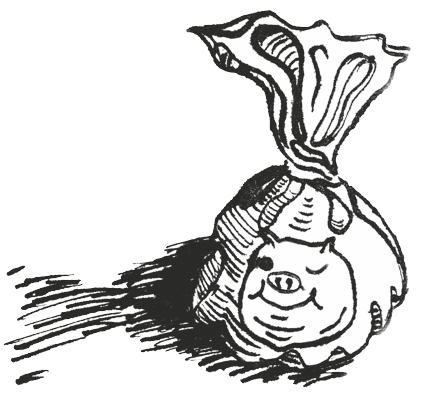
\includegraphics[height=2.2cm]{images/salo.png}\vspace*{-2.21cm}\\
  \hspace*{5mm}Świńskie sadło zatopione w czekoladzie	\\
  \hspace*{5mm}Nie odejdziesz nim spróbujesz			\\
  \hspace*{5mm}Musisz zjeść co najmniej pół			\\
  \hspace*{5mm}Za to w domu zasyp nimi cały stół		\\

  Jakie podać sadełko? Kusi morze wariacji\\
  Wybierz mądrze nadzienie, zrezygnujesz z kolacji\\
  Śliwki, orzech czy chilli, może wolisz sauté\\
  Albo piękną kelnerkę - Olgę!\\
  \\
  Spacerując po bruku z sadłem w swoich kieszeniach\\
  Skoncentrujesz na sobie wygłodniałe spojrzenia\\
  Wnet cię apasz dopadnie; zbity padniesz bez sił\\
  Warknie czule do ucha: E, chcesz w ryj?\\
\end{minipage}
\begin{minipage}[t]{0.2\textwidth}
  a G\\
  F E\\
  a G\\
  F E\\

  a G\\
  F E\\
  F E\\
  F E\\

  a G\\
  F E\\
  a G\\
  F E\\

  a G\\
  F E\\
  a G\\
  F E\\
\end{minipage}

% \newpage
\section{Scenariusz dla moich sąsiadów}\textcolor{lightgray}{\textit{Myslovitz}}\\~\\
\begin{minipage}[t]{0.8\textwidth}
  Kiedy powrócisz już ja będę czekał\\
  Ulicą pójdę wzdłuż kupię gazetę\\
  Zabiorę z sobą psa usiądę na ławce\\
  Skończę scenariusz by gotowy był\\
  Wieczorem...\\
  \\
  \hspace*{5mm}Wieczorem przed mym domem\\
  \hspace*{5mm}Wystawię ekran i wyświetlę film\\
  \hspace*{5mm}Coś o mnie i o tobie\\
  \hspace*{5mm}Będę leczył chore sąsiadów sny\\

  \hspace*{8mm}O oo o o o o...\\
  \\
  Z nieba przyleciał mój wielki przyjaciel\\
  Kiedy lądował ja jadłem kanapkę\\
  Wyśnił że chyba jest chorym człowiekiem\\
  Usiądź wygodnie i nie martw się bo wieczorem\\
\end{minipage}
\begin{minipage}[t]{0.2\textwidth}
  A cis G F E\\
  A cis G F E\\
  A cis G F E\\
  A cis G F E\\

  ~\\
  C E\\
  F F\\
  C E\\
  F F (C E)\\

  A cis G F E $/ \times$2\\

  A cis G F E\\
  A cis G F E\\
  A cis G F E\\
  A cis G F E\\

\end{minipage}

\newpage
\section{Sen Katarzyny II}\textcolor{lightgray}{\textit{Jacek Kaczmarski}}\\~\\
\begin{minipage}[t]{0.85\textwidth}
  Na smyczy trzymam filozofów Europy\\
  Podparłam armią marmurowe Piotra stropy\\
  Mam psy, sokoły, konie - kocham łów szalenie\\
  A wokół same zające i jelenie\\
  \hspace*{6cm}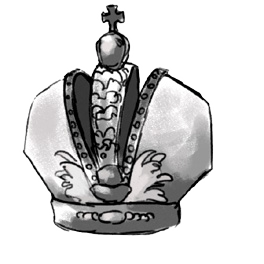
\includegraphics[height=1.5cm]{images/sen_katarzyny_1.png}\vspace*{-1.6cm}\\
  Pałace stawiam, głowy ścinam\\
  Kiedy mi przyjdzie na to chęć\\
  Mam biografów, portrecistów\\
  I jeszcze jedno pragnę mieć\\
  \\
  \hspace*{5mm}Stój Katarzyno! Koronę Carów\\
  \hspace*{5mm}Sen taki jak ten może ci z głowy zdjąć\\
  \\
  Kobietą jestem ponad miarę swoich czasów\\
  Nie bawią mnie umizgi bladych lowelasów\\
  Ich miękkich palców dotyk budzi obrzydzenie\\
  Już wolę łowić zające i jelenie\\
  Ze wstydu potem ten i ów\\
  \hspace*{6cm}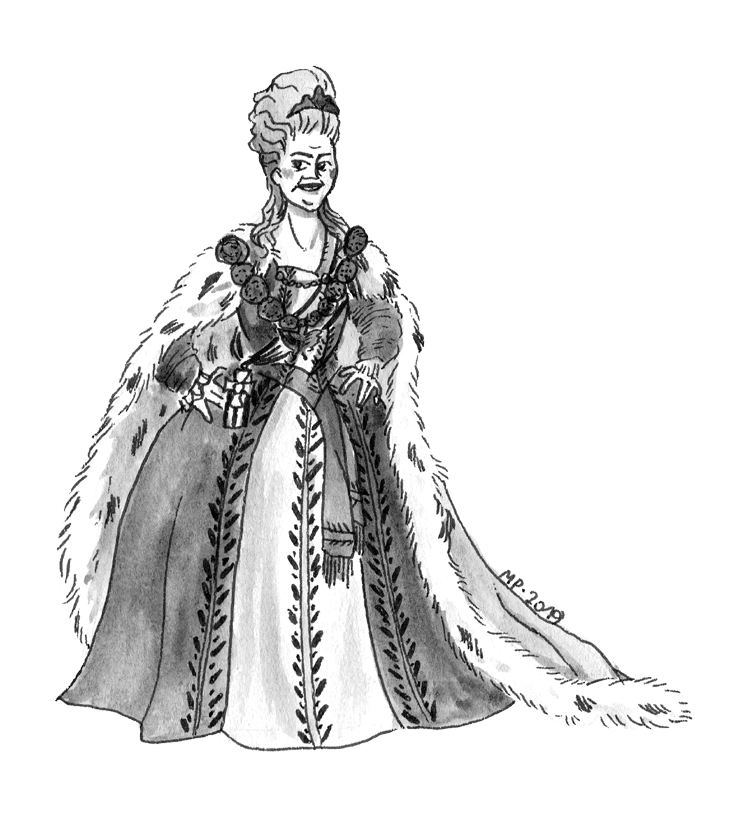
\includegraphics[height=6cm]{images/sen_katarzyny_2.png}\vspace*{-6.1cm}\\
  Rzekł o mnie: niewyżyta niemra!\\
  I pod batogiem nago biegł\\
  Po śniegu, dookoła Kremla\\
  \\
  Kochanka trzeba mi takiego, jak imperium\\
  Co by mnie brał tak jak ja daję - całą pełnią\\
  Co by i władcy i poddańca był wcieleniem\\
  I mi zastąpił zające i jelenie\\
  Co by zrozumiał tak jak ja\\
  Ten głupi dwór rozdanych ról\\
  I pośród pochylonych głów\\
  Dawał mi rozkosz albo ból\\

  \hspace*{5mm}Gdyby się taki kochanek kiedyś znalazł\\
  \hspace*{5mm}Wiem, sama wiem! Kazałabym go ściąć\\

  \hspace*{3mm}Wstań Katarzyno! Pojedź na tekat\\
  \hspace*{3mm}My, tak jak i ty, nienawidzimy gór\\

\end{minipage}
\begin{minipage}[t]{0.15\textwidth}
  G D G\\
  G D e\\
  C D e\\
  C D G\\
  fis   h\\
  fis G   D\\
  C D e\\
  C D G\\

  e H e H\\
  e a C D G\\

  G D G\\
  G D e\\
  C D e\\
  C D G\\
  fis   h\\
  fis G   D\\
  C D e\\
  C D G\\

  G D G\\
  G D e\\
  C D e\\
  C D G\\
  fis   h\\
  fis G   D\\
  C D e\\
  C D G\\

  e H e H\\
  e a C D G\\

  e H e H\\
  e a C D G\\
\end{minipage}

\newpage
\section{Sielanka o domu}\textcolor{lightgray}{\textit{WGB}}\\~\\
\begin{minipage}[t]{0.65\textwidth}
  A jeśli dom będę miał\\
  To będzie bukowy koniecznie\\
  Pachnący i słoneczny\\
  Wieczorem usiądę - wiatr gra\\
  A zegar na ścianie gwarzy\\
  Dobrze się idzie, panie zegarze?\\
  Tik, tak... tik, tak... tik, tak...\\
  Świeca skwierczy i mruga przewrotnie\\
  Więc puszczam oko do niej\\
  Dobry humor dziś pani ma\\
  Dobry humor dziś pani ma\\
  \\
  \hspace*{6mm}Szukam, szukania mi trzeba\\
  \hspace*{6mm}Domu gitarą i piórem\\
  \hspace*{6mm}A góry nade mną, jak niebo\\
  \hspace*{5.5cm}\includegraphics[height=6.5cm]{images/sielanka_o_domu.png}\vspace*{-6.6cm}\\
  \hspace*{6mm}A niebo nade mną, jak góry\\
  \\
  Gdy głosy usłyszę u drzwi\\
  Czyjekolwiek- wejdźcie, poproszę\\
  Jestem zbieraczem głosów\\
  A dom mój bardzo lubi, gdy\\
  Śmiech ściany mu rozjaśnia\\
  I gędźby lubi i pieśni\\
  Wpadnijcie na parę chwil\\
  Kiedy los was zawiedzie w te strony\\
  Bo dom mój otworem stoi\\
  Dla takich jak my\\ dla takich jak wy\\
  \\
  Zaproszę dzień i noc\\
  Zaproszę cztery wiatry\\
  Dla wszystkich drzwi otwarte\\
  Ktoś poda pierwszy ton\\
  Zagramy na góry koncert\\
  Buków porą pachnącą\\
  Nasiąkną ściany grą\\
  A zmęczonym wędrownikom\\
  Odpocząć pozwolą muzyką\\
  Bo taki będzie mój dom $\times 3$\\

\end{minipage}
\begin{minipage}[t]{0.35\textwidth}
  A h$^7$ cis$^7$ A$^7$\\
  D E$^7$ A\\
  h$^7$ E$^7$ cis$^7$ A$^7$\\
  D E E$^7$\\
  A D E\\
  A h$^7$ cis$^7$\\
  h$^7$ E$^7$ A A$^7$\\
  D E E$^7$\\
  A h$^7$ cis$^7$\\
  h$^7$ E cis$^7$ \\
  h$^7$ E A\\

  A E \\
  G D A\\
  A E \\
  G D (d) A\\

  ~\\
  ~\\
  ~\\
  ~\\
  ~\\
  ~\\
  ~\\
  ~\\
  ~\\
  ~\\
  ~\\

  A h$^7$ cis$^7$ A$^7$\\
  D E$^7$ A\\
  h$^7$ E$^7$ cis$^7$ A$^7$\\
  D E E$^7$\\
  A D E\\
  A h$^7$ cis$^7$\\
  h$^7$ E$^7$ A A$^7$\\
  D E E$^7$\\
  A h$^7$ cis$^7$\\
  h$^7$ E cis$^7$, h$^7$ E cis$^7$, h$^7$ E A\\
\end{minipage}

\newpage
\section{Smoke on the water}\textcolor{lightgray}{\textit{Deep Purple}}\\~\\
\begin{minipage}[t]{1\textwidth}
  We all came out to Montreux on the Lake Geneva shoreline\hfill e\\
  To make records with a mobile, we didn't have much time\\
  Frank Zappa and the Mothers were at the best place around\\
  But some stupid with a flare gun burned the place to the ground\\

  \hspace*{5mm}Smoke on the water, fire in the sky\\
  \hspace*{5mm}Smoke on the water\\

  They burned down the gambling house, it died with an awful sound\\
  Funky Claude was running in and out, pulling kids out the ground\\
  When it all was over, we had to find another place\\
  But Swiss time was running out, it seemed that we would lose the race\\

  We ended up at the Grand hotel, it was empty cold and bare\\
  But with the Rolling truck Stones thing just outside, making our music there\\
  With a few red lights and a few old beds, we make a place to sweat\\
  No matter what we get out of this, I know we'll never forget\\
\end{minipage}
\begin{minipage}[t]{0\textwidth}
\end{minipage}

\newpage
\section{Society}\textcolor{lightgray}{\textit{Eddie Vedder}}\\~\\
\begin{minipage}[t]{0.9\textwidth}
  It's a mystery to me \\
  We have a greed with which we have agreed\\
  And you think you have to want more than you need \\
  Until you have it all, you won't be free\\
  \\
  \hspace*{5mm}Society, you're crazy breed \\
  \hspace*{5mm}I hope you're not lonely without me\\
  \\
  When you want more than you have, you think you need\\
  And when you think more than you want, your thoughts begin to bleed\\
  I think I need to find a bigger place\\
  Cause when you have more than you think, you need more space\\
  \\
  \hspace*{5mm}Society, you're crazy breed\\
  \hspace*{5mm}I hope you're not lonely without me\\
  \hspace*{5mm}Society, crazy indeed\\
  \hspace*{5mm}Hope you're not lonely without me\\
  \\
  There's those thinking more or less, less is more\\
  But if less is more, how you keepin' score?\\
  Means for every point you make your level drops\\
  Kinda like you're startin' from the top\\
  And you can't do that\\
  \\
  \hspace*{5mm}Society, you're a crazy breed\\
  \hspace*{5mm}I hope you're not lonely without me\\
  \hspace*{5mm}Society, crazy indeed\\
  \hspace*{5mm}I hope you're not lonely without me\\
  \hspace*{5mm}Society, have mercy on me\\
  \hspace*{5mm}I hope you're not angry if I disagree\\
  \hspace*{5mm}Society, you're crazy indeed\\
  \hspace*{5mm}I hope you're not lonely without me\\
\end{minipage}
\begin{minipage}[t]{0.1\textwidth}
  G D G\\
  G C D\\
  C D e\\
  C D e\\

  C G\\
  D e\\

  G D G\\
  G C D\\
  C D e\\
  C D e\\

  C G\\
  D e\\
  C G\\
  D e\\

  G D G\\
  G C D\\
  C D e\\
  C D e\\
  \\
  \\
  C G\\
  D e\\
  C G\\
  D e\\
  C G\\
  D e\\
  C G\\
  D e\\

\end{minipage}

\newpage
\section{Somewhere over the rainbow}\textcolor{lightgray}{\textit{Israel Kamakawiwo'ole}}\\~\\
\begin{minipage}[t]{0.7\textwidth}
  ~\\~\\
  Somewhere over the rainbow\\
  Way up high\\
  And the dreams that you dreamed of\\
  Once in a lullaby\\

  Oh, somewhere over the rainbow\\
  Blue birds fly\\
  And the dreams that you dreamed of\\
  Dreams really do come true, ooh-ooh\\

  \hspace*{5mm}Someday I'll wish upon a star\\
  \hspace*{5mm}Wake up where the clouds are far behind \\
  \hspace*{5mm}me\\
  \hspace*{5mm}Where trouble melts like lemon drops\\
  \hspace*{5mm}High above the chimney tops, that's where\\
  \hspace*{5mm}You'll find me\\

  Oh, somewhere over the rainbow\\
  Blue birds fly\\
  And the dream that you dare to\\
  Oh, why, oh, why can't I?\\
\end{minipage}
\begin{minipage}[t]{0.3\textwidth}
  C e F C\\
  F E$^7$ a F\\
  C e\\
  F C\\
  F C\\
  G a F\\

  C e\\
  F C\\
  F C\\
  G a F\\

  C\\
  e a\\
  F\\
  C\\
  e a\\
  F\\

  C e\\
  F C\\
  F C\\
  G a F\\
\end{minipage}

\newpage
\section{Stand by me / Every breath you take / I just called to say I love you}\textcolor{lightgray}{\textit{}}\\~\\
\begin{minipage}[t]{0.85\textwidth}
  When the night has come and the land is dark\\
  And the moon is the only light we'll see\\
  No, I won't be afraid, no, I won't be afraid\\
  Just as long as you stand, stand by me\\
  \\
  \hspace*{5mm}So, darling, darling, stand by me, oh, stand by me\\
  \hspace*{5mm}Stand by me, stand by me, stand by me\\
  \hspace*{5mm}Whenever something's going wrong / you're in trouble won't you\\
  \hspace*{5mm}Stand by me, oh, stand by me\\
  \hspace*{5mm}Stand by me, stand by me, stand by me\\

  If the sky that we look upon should tumble and fall\\
  Or the mountain should crumble in the sea\\
  I won't cry, I won't cry, no, I won't shed a tear\\
  Just as long as you stand, stand by me\\

  ---\\

  Every breath you take, every move you make\\
  Every bond you break, every step you take				\\
  I'll be watching you							\\
  Every single day, every word you say\\
  Every game you play, every night you stay\\
  I'll be watching you\\
  \hspace*{5mm}Oh, can't you see, you belong to me				\\
  \hspace*{5mm}How my poor heart aches with every step you take	\\

  Every move you make, every vow you break\\
  Every smile you fake, every claim you stake\\
  I'll be watching you\\

\end{minipage}
\begin{minipage}[t]{0.15\textwidth}
  C a\\
  F G C\\
  C a\\
  F G C\\

  C a\\
  F G C\\
  C\\
  C a\\
  F G C\\

  C a\\
  F G C\\
  C a\\
  F G C\\

  ~\\

  C a\\
  F G\\
  a\\
  C a\\
  F G\\
  a\\
  F C\\
  D G\\

  C a\\
  F G\\
  a\\

\end{minipage}
\newpage
\begin{minipage}[t]{0.75\textwidth}
  ---\\

  No New Year's Day to celebrate 					\\
  No chocolate covered candy hearts to give away 			\\
  No first of spring, no song to sing 				\\
  In fact here's just another ordinary day\\
  No April rain, no flowers bloom\\
  No wedding Saturday within the month of June\\
  But what it is, is something true\\
  Made up of these three words that I must say to you\\
  \hspace*{7.4cm}\includegraphics[height=2.5cm]{images/stand_by_me.png}\vspace*{-2.6cm}\\
  \\
  \hspace*{5mm}I just called to say I love you 		\\
  \hspace*{5mm}I just called to say how much I care\\
  \hspace*{5mm}I just called to say I love you 		\\
  \hspace*{5mm}And I mean it from the bottom of my heart\\
  \\
  No summer's high, no warm July 				\\
  No harvest moon to light one tender August night 		\\
  No autumn breeze, no falling leaves 			\\
  Not even time for birds to fly to southern skies\\
  No Libra sun, no Halloween\\
  No giving thanks for all the Christmas joy you bring\\
  But what it is, though old so new\\
  To fill your heart like no three words could ever do\\
\end{minipage}
\begin{minipage}[t]{0.25\textwidth}
  ~\\~\\
  C\\
  C d\\
  d d$^{7+}$ d$^7$ d$^{7+}$\\
  d G C\\
  C\\
  C d\\
  d d$^{7+}$ d$^7$ d$^{7+}$\\
  d G C\\

  F G C\\
  F G a\\
  F G a\\
  F G C\\

  C\\
  C d\\
  d d$^{7+}$ d$^7$ d$^{7+}$\\
  d G C\\
  C\\
  C d\\
  d d$^{7+}$ d$^7$ d$^{7+}$\\
  d G C\\
\end{minipage}

% \newpage
\section{Stand by your man}\textcolor{lightgray}{\textit{Tammy Wynette / The Blues Brothers}}\\~\\
\begin{minipage}[t]{0.7\textwidth}
  Sometimes it's hard to be a woman\\
  Giving all your love to just one man\\
  And if you love him, oh, be proud of him\\
  'Cause after all he's just a man\\
  \\
  \hspace*{5mm}Stand by your man\\
  \hspace*{5mm}Give him two arms to cling to\\
  \hspace*{5mm}And something warm to come to\\
  \hspace*{5mm}When nights are cold and lonely\\
  \hspace*{5mm}Stand by your man\\
  \hspace*{5mm}And tell the world you love him\\
  \hspace*{5mm}Keep givin' all the love you can\\
  \hspace*{5mm}Baby, stand by your man\\
\end{minipage}
\begin{minipage}[t]{0.3\textwidth}
  C G\\
  d G$^7$ C C$^7$\\
  F C a\\
  d G$^7$ C (F C G)\\

  C E$^7$\\
  F\\
  C A$^7$\\
  D$^7$ G$^7$\\
  C E$^7$\\
  F\\
  C G$^7$ E$^7$ A$^7$\\
  F G C\\
\end{minipage}

\newpage
\section{Starless}\textcolor{lightgray}{\textit{King Crimson}}\\~\\
\begin{minipage}[t]{0.65\textwidth}
  Sundown dazzling day\\
  Gold through my eyes\\
  But my eyes turned within, only see\\
  Starless and bible black\\
  \\
  Old friend charity\\
  Cruel twisted smile\\
  And the smile signals emptiness for me\\
  Starless and bible black\\
  \\
  Ice blue, silver sky\\
  Fades into grey\\
  To a grey hope that oh yearns to be\\
  Starless and bible black\\
\end{minipage}
\begin{minipage}[t]{0.35\textwidth}
  a E \\
  E a \\
  C G a\\
  a E a\\

  a E \\
  E a \\
  C G a\\
  a E a\\

  a E \\
  E a \\
  C G a\\
  a E a\\
\end{minipage}
~\\~\\~\\~\\~\\
\includegraphics[width = \textwidth, center]{starless.png}\\

\newpage
\section{Szczęśliwej drogi już czas}\textcolor{lightgray}{\textit{Ryszard Rynkowski}}\\~\\
\begin{minipage}[t]{0.8\textwidth}
  Los cię w drogę pchnął i ukradkiem drwiąc się, śmiał\\
  Bo nadzieję dając ci, fałszywy klejnot dał\\
  A ty, idąc w świat, patrzysz w klejnot ten co dnia\\
  Chociaż rozpacz już od lat wyziera z jego dna\\
  Uuuuuu… z jego dna\\
  \\
  Na rozstaju dróg, gdzie przydrożny Chrystus stał\\
  Zapytałeś, dokąd iść, frasobliwą minę miał\\
  Przystanąłeś więc z płaczem brzóz sprzymierrzyć się\\
  I uronić pierwszy raz w czerwone wino łzę\\
  ~\\
  \\
  \hspace*{5mm}Szczęśliwej drogi już czas\\
  \hspace*{5mm}Mapę życia w sercu masz\\
  \hspace*{5mm}Jesteś jak młody ptak\\
  \hspace*{5mm}Głuchy jest los\\
  \hspace*{5mm}Nadaremnie wzywasz go\\
  \hspace*{5mm}Bo twój głos\\
  \\
  Idziesz wiecznie sam i już nic nie zmieni się\\
  Poza tym, że raz jest za, raz przed tobą jest twój cień\\
  Los cię w drogę pchnął i ukradkiem drwiąc się, śmiał\\
  Bo nadzieję dając ci, fałszywy klejnot dał\\
  ~\\
\end{minipage}
\begin{minipage}[t]{0.2\textwidth}
  a E\\
  F E\\
  a E\\
  F E\\
  G d a\\

  a E\\
  F E\\
  a E\\
  F E\\
  G d a\\

  C\\
  G\\
  d a\\
  C\\
  G\\
  d\\

  a E\\
  F E\\
  a E\\
  F E\\
  G d a\\
\end{minipage}

% \newpage
\section{Świtezianka}\textcolor{lightgray}{\textit{Mumio}}\\~\\
\begin{minipage}[t]{0.8\textwidth}
  Cóż to za chłopak piękny i młody? Cóż to za obok dziewica?\\
  Tu, nad brzegami Świtezi wody, gonią się po ulicach\\
  Ona mu z kosza daje ostrężyny, a on jej kwiaty do wianka\\
  \vspace*{10mm}\hspace*{10cm}\includegraphics[height=2.8cm]{switezianka.png}\vspace*{-3.2cm}\\
  Pewnie kochankiem jest tej dziewczyny, pewnie to jego nałożnica\\
  \hspace*{8.5cm}\includegraphics[height=3cm]{switezianka2.png}\vspace*{-3.1cm}\\
  \\
  \hspace*{5mm}Ucha ucha, taniec brzucha, ucha ucha Świtezianka\\
\end{minipage}
\begin{minipage}[t]{0.2\textwidth}
  A$^7$ D$^7$\\

\end{minipage}

\newpage
\section{Take me as i am}\textcolor{lightgray}{\textit{Tedeschi Trucks Band}}\\~\\
\begin{minipage}[t]{0.8\textwidth}
  Take me as I am, for I am just like you\\
  We're made from the same hand, born of the same land\\
  Take me as I am. I haven't said a word\\
  The dreams I have are real, no matter how absurd\\

  \hspace*{5mm}Life is just a wish, some of us hold dear\\
  \hspace*{5mm}Tethered by a thread, held back by our fears\\
  \hspace*{5mm}No matter where you're from, all that you can do\\
  \hspace*{5mm}Is live in love - that's enough\\

  Take me as I am, I feel you in my heart\\
  We fill the same space, no matter how far apart\\
  Take me as I am, for I am just like you\\
  You're a part of me and I'm a part of you\\

  \hspace*{5mm}Oh, why can't we share this world?\\
  \hspace*{5mm}There is always room for those who dare to love\\
  \hspace*{5mm}Meet me with a smile and I will be your friend\\
  \hspace*{5mm}And care for you 'til the end\\

  Take me as I am, for I am just like you\\
  You're a part of me, I'm a part of you\\
  Oh, don't take away my life, 'cause we're made from the same sky\\
  We've shared a trail of tears way too many years\\

  You're a part of me, I'm a part of you\\
  You're a part of me, take me as I am\\

\end{minipage}
\begin{minipage}[t]{0.2\textwidth}
  G h$^7$\\
  a$^7$ e D\\
  G h$^7$\\
  a$^7$ C e D\\

  a$^7$ D\\
  G C\\
  a$^7$ F\\
  C  D \\

  G D\\
  a$^7$ e D\\
  G D\\
  a$^7$ C e D\\

  a$^7$ D\\
  G C\\
  a$^7$ F\\
  C  D \\

  G D\\
  a$^7$ e D\\
  G D\\
  a$^7$ C e D\\

  D\\
\end{minipage}

\newpage
\section{Takie tango}\textcolor{lightgray}{\textit{Budka Suflera}}\\~\\
\begin{minipage}[t]{0.8\textwidth}
  Na sali wielkiej i błyszczącej tak jak nocne Buenos Aires\\
  Które nie chce spać \\
  Orkiestra stroi instrumenty, daje znak i zaraz zacznie\\
  Nowe tango grać\\
  Siedzimy obok obojętni wobec siebie jak turyści\\
  Wystukując rytm\\
  Nie będzie tanga między nami, choćby nawet cud się ziścił\\
  Nie pomoże nic\\
  \\
  \hspace*{3mm}Chociaż płyną ostre nuty, w żyłach płonie krew \\
  \hspace*{3mm}Nigdy żadne z nas do tańca nie poderwie się\\
  \\
  \hspace*{6mm}Bo do tanga trzeba dwojga zgodnych ciał i chętnych serc\\
  \hspace*{6mm}Bo do tanga trzeba dwojga, tak ten świat złożony jest\\
  \\
  \\
  Zaleje w końcu Buenos Aires noc tak gęsta jak atrament\\
  A gdy przyjdzie brzask\\
  Co było w naszych sercach kiedyś, kiedyś jak świecący diament\\
  Cały straci blask\\
  \\
  \hspace*{3mm}I choć będą znowu grali, Bóg to jeden wie\\
  \hspace*{3mm}Nigdy razem na tej sali nie spotkamy się\\
\end{minipage}
\begin{minipage}[t]{0.2\textwidth}
  d\\
  B A d\\
  d\\
  B A d\\
  d\\
  B A d\\
  d\\
  B A d\\
  \\
  g F C\\
  g F C\\
  (A)\\
  d A | $\times$4\\
  d A | $\times$3\\
  (d B d A d) x2\\

  d\\
  B A d\\
  d\\
  B A d\\
  \\
  g F C\\
  g F C\\
\end{minipage}
~\\
~\\
\includegraphics[height=7cm, center]{takie_tango.png}\\

\newpage
\section{Tears in heaven}\textcolor{lightgray}{\textit{Eric Clapton}}\\~\\
\begin{minipage}[t]{0.7\textwidth}
  Would you know my name?\\
  If I saw you in heaven\\
  Would it be the same?\\
  If I saw you in heaven\\
  \hspace*{3mm}I must be strong\\
  \hspace*{3mm}And carry on\\
  \hspace*{3mm}'Cause I know I don't belong\\
  \hspace*{3mm}Here in heaven\\

  Would you hold my hand?\\
  If I saw you in heaven\\
  Would you help me stand?\\
  If I saw you in heaven\\
  \hspace*{3mm}I'll find my way\\
  \hspace*{3mm}Through night and day\\
  \hspace*{3mm}'Cause I know I just can't stay\\
  \hspace*{3mm}Here in heaven\\

  \hspace*{8mm}Time can bring you down\\
  \hspace*{8mm}Time can bend your knees\\
  \hspace*{8mm}Time can break your heart\\
  \hspace*{8mm}Have you begging please\\
  \hspace*{8mm}Begging please\\

  \hspace*{3mm}Beyond the door\\
  \hspace*{3mm}There's peace, I'm sure\\
  \hspace*{3mm}And I know there'll be no more\\
  \hspace*{3mm}Tears in heaven\\

\end{minipage}
\begin{minipage}[t]{0.3\textwidth}
  A E fis A\\
  D A E\\
  A E fis A\\
  D A E\\
  fis Cis\\
  A$^7$ fis$^7$\\
  h$^7$\\
  A\\

  A E fis A\\
  D A E\\
  A E fis A\\
  D A E\\
  fis Cis\\
  A$^7$ fis$^7$\\
  h$^7$\\
  A\\

  C $\star$ a$^7$\\
  D G D e DG\\
  C $\star$ a$^7$\\
  D G D \\
  E\\
  (A E fis A D A E $\times 2$)\\
  fis Cis\\
  A$^7$ fis$^7$\\
  h$^7$\\
  A\\
\hspace*{-0.4cm}\vspace*{-1.4cm}
  \chord{t}{x,p2,n,n,p3,x}{$\star$}
\end{minipage}

\newpage
\section{Teksański}\textcolor{lightgray}{\textit{Hey}}\\~\\
\begin{minipage}[t]{0.7\textwidth}
  ~\\ % pusta linia jeśli jest intro
  Herbata stygnie, zapada zmrok,\\
  a pod piórem ciągle nic\\
  Obowiązek obowiązkiem jest,\\
  piosenka musi posiadać tekst\\
  Gdyby chociaż mucha zjawia się,\\
  mogłabym ją zabić\\
  A później to opisać\\
  \includegraphics[height = 2cm,right]{teksanski.png}\vspace*{-2.1cm}\\
  \\
  W moich słowach słoma czai się,\\
  nie znaczą nic\\
  Jeśli szukasz sensu, prawdy w nich -\\
  zawiedziesz się\\
  \\
  A może zmienić zasady gry?\\
  Chcesz usłyszeć słowa,\\
  to sam je sobie wymyśl\\
  \\
  Nabij diabla, chmurę śmierci weź -\\
  pomoże Ci \\
  Wnet twe myśli w słowa zmienią się,\\
  wyśpiewasz je sam.\\

\end{minipage}
\begin{minipage}[t]{0.3\textwidth}
  D G A   \\ % intro
  D G A \\
  D G A \\
  D G A \\
  D G A \\
  D G A \\
  D G A \\
  D G A \\
  \\
  G A D \\
  G A D \\
  G A D \\
  G A \\
  \\
  D G A \\
  D G A \\
  D G A \\
  \\
  G A D \\
  G A D \\
  G A D \\
  G A \\
  (D G A) \\

\end{minipage}

\newpage
\section{The sound of silence}\textcolor{lightgray}{\textit{Simon \& Garfunkel}}\\~\\
\begin{minipage}[t]{0.7\textwidth}
  ~\\
  Hello darkness, my old friend\\
  I've come to talk with you again\\
  Because a vision softly creeping\\
  Left its seeds while I was sleeping\\
  And the vision that was planted in my brain\\
  Still remains\\
  Within the sound of silence\\
  \\
  In restless dreams I walked alone\\
  Narrow streets of cobblestone\\
  `Neath the halo of a street lamp\\
  I turned my collar to the cold and damp\\
  When my eyes were stabbed by the flash of a neon light\\
  That split the night\\
  And touched the sound of silence\\
  \\
  And in the naked light I saw\\
  Ten thousand people, maybe more\\
  People talking without speaking\\
  People hearing without listening\\
  People writing songs that voices never share\\
  No one dared\\
  Disturb the sound of silence\\
  \\
  ``Fools'' said I, ``You do not know\\
  Silence like a cancer grows\\
  Hear my words that I might teach you\\
  Take my arms that I might reach you''\\
  But my words like silent raindrops fell\\
  And echoed in the wells of silence\\
  \\
  And the people bowed and prayed\\
  To the neon god they made\\
  And the sign flashed out its warning\\
  In the words that it was forming\\
  And the sign said, ``The words of the prophets\\
  Are written on the subway walls\\
  And tenement halls\\
  And whispered in the sounds of silence''\\
\end{minipage}
\begin{minipage}[t]{0.15\textwidth}
  (E$^2$)\\
  e D\\
  D e\\
  e CG\\
  G CG (G)\\
  C C G\\
  Ge (G)\\
  D e e\\

  D\\
  D e\\
  e CG\\
  G CG (G)\\
  C C G\\
  Ge (G)\\
  D e e\\

  D\\
  D e\\
  e CG\\
  G CG (G)\\
  C C G\\
  Ge (G)\\
  D e e\\

  D\\
  D e\\
  e CG\\
  G CG (G)\\
  C C G (Ge)\\
  G D e e\\

  D\\
  D e\\
  e CG\\
  G CG\\
  G C\\
  C G\\
  Ge\\
  G D e e\\
\end{minipage}
\begin{minipage}[t]{0.15\textwidth}
  (A$^2$) {\scriptsize \textit{[capo 6]}}\\
  A$^2$ G \\
  G a\\
  a FC\\
  C FC (C)\\
  F F C\\
  Ca (C)\\
  G a a\\

  G \\
  G a\\
  a FC\\
  C FC (C)\\
  F F C\\
  Ca (C)\\
  G a a\\

  G \\
  G a\\
  a FC\\
  C FC (C)\\
  F F C\\
  Ca (C)\\
  G a a\\

  G \\
  G a\\
  a FC\\
  C FC (C)\\
  F F C (Ca)\\
  C G a a\\

  G \\
  G a\\
  a FC\\
  C FC\\
  C F\\
  F C\\
  Ca\\
  C G a a\\

\end{minipage}

\newpage
\section{TNT}\textcolor{lightgray}{\textit{AC/DC}}\\~\\
\begin{minipage}[t]{0.7\textwidth}
  See me ride out of the sunset on your color TV screen\\
  Out for all that I can get - if you know what I mean\\
  Women to the left of me, women to the right\\
  Ain't got no gun, ain't got no knife, don't you start no fight\\
  \\
  \hspace*{5mm}'Cause I'm TNT - I'm dynamite \\
  \hspace*{5mm}TNT - and I'll win the fight\\
  \hspace*{5mm}TNT - I'm a power load\\
  \hspace*{5mm}TNT - watch me explode\\
  \\
  I'm dirty, mean and mighty unclean, I'm a wanted man\\
  Public enemy number one - Understand\\
  So lock up your daughter, lock up your wife\\
  Lock up your back door and run for your life\\
  The man is back in town, don't you mess me 'round\\
\end{minipage}
\begin{minipage}[t]{0.3\textwidth}
  E G A (G A G) | $\times$2\\
  \\
  \\
  \\
  \\
  A G E G A
\end{minipage}

\newpage
\section{Tolerancja}\textcolor{lightgray}{\textit{Stanisław Soyka}}\\~\\
\begin{minipage}[t]{0.75\textwidth}
  Dlaczego nie mówimy o tym co nas boli otwarcie\\
  Budować ściany wokół siebie marna sztuka\\
  Wrażliwe słowo czuły dotyk wystarczą\\
  Czasami tylko tego pragnę tego szukam\\

  \hspace*{5mm}Na miły Bóg\\
  \hspace*{5mm}Życie nie tylko po to jest by brać\\
  \hspace*{5mm}Życie nie po to by bezczynnie trwać\\
  \hspace*{5mm}I aby żyć siebie samego trzeba dać\\

  Problemy twoje moje nasze boje polityka\\
  A przecież każdy włos jak nasze lata policzony\\
  Kto jest bez winy niechaj pierwszy rzuci kamień niech rzuci\\
  Daleko raj gdy na człowieka się zamykam\\

\end{minipage}
\begin{minipage}[t]{0.25\textwidth}
  D A\\
  A D\\
  D A\\
  D G A D A D\\

  A\\
  D G A\\
  D G A\\
  D G A\\

  D A\\
  A D\\
  D A\\
  D G A D A D\\

\end{minipage}

% \newpage
\section{Tyle słońca w całym mieście}\textcolor{lightgray}{\textit{Anna Jantar}}\\~\\
\begin{minipage}[t]{0.8\textwidth}
  Dzień - wspomnienie lata, dzień - słoneczne ćmy, a-a!\\
  Nagle w tłumie, w samym środku miasta\\
  Ty, po prostu ty\\
  \\
  Dzień - godzina zwierzeń, dzień - przy twarzy twarz, a-a!\\
  Szuka pamięć poplątanych ścieżek\\
  Lecz czy znajdzie nas?\\
  \\
  Tyle słońca w całym mieście, nie widziałeś tego jeszcze\\
  Popatrz, o, popatrz!\\
  Szerokimi ulicami niosą szczęście zakochani\\
  Popatrz, o, popatrz!\\
  Wiatr porywa ich spojrzenia, biegnie światłem w smugę cienia\\
  Popatrz, o, popatrz!\\
  Łączy serca, wiąże dłonie, może nam zawróci w głowie też\\
  \\
  Dzień - powrotna podróż, dzień - podanie rąk, a-a!\\
  Ale niebo całe jeszcze w ogniu\\
  Chcę zatrzymać wzrok\\
\end{minipage}
\begin{minipage}[t]{0.2\textwidth}
  d A$^7$ d D$^7$\\
  g d\\
  E$^7$ A$^7$\\

  d A$^7$ d D$^7$\\
  g d\\
  E$^7$ A$^7$\\
  \\
  d\\
  g\\
  A$^7$\\
  d\\
  D$^7$\\
  g\\
  A$^7$ d\\

  d A$^7$ d D$^7$\\
  g d\\
  E$^7$ A$^7$\\

\end{minipage}

\newpage
\section{Uciekaj moje serce}\textcolor{lightgray}{\textit{Seweryn Krajewski
  }}\\~\\
\begin{minipage}[t]{0.8\textwidth}
  Gdzieś w hotelowym korytarzu krótka chwila\\
  Splecione ręce, gdzieś na plaży oczu błysk\\
  Wysłany w biegu krótki list, stokrotka śniegu, dobra myśl\\
  To wciąż za mało, moje serce, żeby żyć\\
  \\
  \hspace*{5mm}Uciekaj skoro świt, bo potem będzie wstyd\\
  \hspace*{5mm}I nie wybaczy nikt chłodu ust, braku słów \\
  \hspace*{5mm}Uciekaj skoro świt, bo potem będzie wstyd\\
  \hspace*{5mm}I nie wybaczy nikt chłodu ust twych\\
  \\
  Burzliwe wtorki, które przyjdą po niedzielach\\
  Kropelka żalu, której winien jesteś ty\\
  Nieprawda, że tak miało być, że warto w byle pustkę iść\\
  To wciąż za mało, moje serce, żeby żyć\\
  \\
  Odloty nagłe i wstydliwe, niezabawne\\
  Nic niewiedzący, a zdradzony pies, czy miś\\
  Żałośnie chuda kwiatów kiść i nowa złuda, nowa nić\\
  To wciąż za mało, moje serce, żeby żyć\\
\end{minipage}
\begin{minipage}[t]{0.2\textwidth}
  a E a\\
  G C\\
  A$^7$ d\\
  G C\\

  d a\\
  E a (A)\\
  d a\\
  E a\\

  a E a\\
  G C\\
  A$^7$ d\\
  G C\\

  a E a\\
  G C\\
  A$^7$ d\\
  G C\\
\end{minipage}

% \newpage
\section{Ukaraj mnie}\textcolor{lightgray}{\textit{Tymon \& Transistors}}\\~\\
\begin{minipage}[t]{0.7\textwidth}
  ~\\
  Wiem, że byłem podły całe życie swe\\
  Wszystko, co robiłem, było podłe i złe\\
  Dzisiaj jestem gotów oddać członki swe\\
  Na wymyślną pastwę zemsty twej\\
  \\
  \hspace*{2mm}Chcę być brudnym mopem u twych drobnych stóp\\
  \hspace*{2mm}Zetrzyj mnie na papkę oraz wygól rów\\
  \hspace*{2mm}Poniżenia łaknę z twoich miłych rąk\\
  \hspace*{2mm}Opij się mą stęchłą krwią jak bąk\\

  \hspace*{6mm}Ukaraj mnie (smyczą, kablem)\\
  \hspace*{6mm}Ukaraj mnie (tego pragnę)\\
  \hspace*{6mm}Ukaraj mnie (odbierz godność)\\
  \hspace*{6mm}Ukaraj mnie (wbij się w mąkość)\\
  \\
  Chcę by dzisiaj wreszcie wydarzyło się\\
  Coś tak potwornego, że aż staje dech\\
  Coś tak straszliwego, że aż czeźnie krew\\
  Rozszarp mnie jak Baskerville'ów pies\\
\end{minipage}
\begin{minipage}[t]{0.13\textwidth}
  ~\\
  a E\\
  E a\\
  a E\\
  E a\\

  a E\\
  E a\\
  a E\\
  E a\\

  d\\
  a\\
  d\\
  E\\

  a E\\
  E a\\
  a E\\
  E a\\
\end{minipage}
\begin{minipage}[t]{0.17\textwidth}
  \textcolor{gray}{\footnotesize [w bieszczadach]}\\
  e a\\
  D G H$^7$\\
  e a\\
  D G H$^7$\\

  G C D G\\
  G C D G\\
  G C D G\\
  G C D G\\(H$^7$)\\

  ~\\~\\~\\

  e a\\
  D G H$^7$\\
  e a\\
  D G H$^7$\\
\end{minipage}

\newpage
\section{Uśmiech śmierci}\textcolor{lightgray}{\textit{Dżem}}\\~\\
\begin{minipage}[t]{0.7\textwidth}
  Gdy o łzę uderza łza, znowu widzę\\
  Twoich ust tak piękny kształt\\
  Jestem teraz, teraz sam, ucichł wokół szum i gwar\\
  Wszyscy ze swoimi lub do swoich poszli żon\\
  \hspace*{4mm}Kto pomoże teraz, kto\\
  \hspace*{4mm}Znaleźć mi w tej ciszy twarz\\
  \hspace*{4mm}Mojej małej, którą dawno już\\
  \hspace*{4mm}Śmierć okrutna zabrała mi\\
  \\
  Pamiętam, pamiętam dobrze ją\\
  Jak weszła przez zamknięte drzwi\\
  Nie mogłem w to uwierzyć, lecz ty wiedziałaś już\\
  Że to śmierć odwiedziła nasz dom\\
  \hspace*{4mm}I krzyczałem: Nie zabieraj jej\\
  \hspace*{4mm}Zostaw małą, zostaw, proszę cię\\
  \hspace*{4mm}Ale ona tylko uśmiechnęła się\\
  \hspace*{4mm}Mówiąc: Ma już tylko mnie\\
  \\
  Siedziałem na twym łóżku, ściskając twoją dłoń\\
  Lecz ona chłodna była już\\
  Potem tylko przez chwilę widziałem taniec twój\\
  Taniec twój ze straszną śmiercią\\
  \hspace*{4mm}Wiem, że ona do wszystkich, do mnie też\\
  \hspace*{4mm}Wejdzie dumnie przez zamknięte drzwi\\
  \hspace*{4mm}I do tańca mnie zaprosi, bym\\
  \hspace*{4mm}Moją małą spotkać mógł\\
\end{minipage}
\begin{minipage}[t]{0.3\textwidth}
  A A$^4$\\
  D D$^4$ A\\
  A A$^4$\\
  D D$^4$ A\\
  fis D\\
  fis D\\
  fis D\\
  G D A\\

  A A$^4$\\
  D D$^4$ A\\
  A A$^4$\\
  D D$^4$ A\\
  fis D\\
  fis D\\
  fis D\\
  G D A\\

  A A$^4$\\
  D D$^4$ A\\
  A A$^4$\\
  D D$^4$ A\\
  fis D\\
  fis D\\
  fis D\\
  G D A\\
\end{minipage}

\newpage
\section{W góry swe jadę}\textcolor{lightgray}{\textit{Paweł Jacyk, Filip Marcinek}}\\~\\
\begin{minipage}[t]{0.6\textwidth}
  W góry swe jadę życia koleją\\
  Przez gęstą mgłę, nie widząc nic wkoło\\
  Uciekam z miasta, gdzie w oczy wieją\\
  Wiatry fortuny, a myśli bolą\\
  \\
  Tam o kamienie się wciąż potykam\\
  Wypełnią miejsce plecaka mego\\
  Z takim bagażem w podróż wyruszam\\
  W górach nie trzeba mi nic innego\\
  \\
  Wchodzę na szczyt, to cel oczywisty\\
  Mojej góry, do której praw nie mam\\
  Świat pozostawiam za sobą mglisty\\
  Gdy na szczyt duszy przez lasy zmierzam\\
  \\
  W końcu docieram tam, gdzie jest cicho\\
  Wyżej nie wejdę, spoglądam w dół\\
  Szczęście to nigdy mi się nie śniło\\
  Żeby swą dłonią dosięgnąć aż chmur\\
  \\
  Jak każda chwila, ta szybko minie\\
  Idę już na dół, plecak zgubiłem\\
  Miłość w mym sercu nigdy nie zginie\\
  Do góry, którą już opuściłem\\
  \\
  \hspace*{4mm}Przecież ty znowu, górski człowieku\\
  \hspace*{4mm}Wracasz do miasta z przepięknych swych gór\\
  \hspace*{4mm}Dlaczego znowu, górski człowieku\\
  \hspace*{4mm}Wracasz do miasta z bezdusznych swych gór\\
  \\
  Wracam, by zebrać nowych kamieni\\
  Znów się poślizgnąć, ale nie upaść\\
  Wzlecieć jak liść na wietrze jesieni\\
  Zmierzając z wolna w rutyny przepaść\\

\end{minipage}
\begin{minipage}[t]{0.4\textwidth}
  d a\\
  F C\\
  B F\\
  B A\\
  \\
  d a\\
  F C\\
  B A\\
  B C d \\

  d a\\
  F C\\
  B F\\
  B A\\
  \\
  d a\\
  F C\\
  B A\\
  B C d \\

  d a  \\
  F C  \\
  B C  \\
  B C F C\\

  F C a d \\
  F C a d \\
  F C a d \\
  F C d a d\\

  d a  \\
  F C  \\
  B C  \\
  B C F C\\
\end{minipage}

\newpage
\section{We wtorek po sezonie}\textcolor{lightgray}{\textit{Wołosatki}}\\~\\
\begin{minipage}[t]{0.7\textwidth}
  Złotym kobiercem wymoszczone góry\\
  Jesień w doliny przyszła dziś nad ranem\\
  Buki czerwienią zabarwiły chmury\\
  Z latem się złotym właśnie pożegnałem\\
  \\
  \hspace*{5mm}We wtorek w schronisku po sezonie\\
  \hspace*{5mm}W doliny wczoraj zszedł ostatni gość\\
  \hspace*{5mm}Za oknem plucha i kubek parzy w dłonie\\
  \includegraphics[height=2cm, right]{we_wtorek_po_sezonie.png}\vspace*{-2.1cm}\\
  \hspace*{5mm}I tej herbaty i tych gór mam dość\\
  \\
  Szaruga niebo powoli zasnuwa\\
  Wiatr już gałęzie pootrząsał z liści\\
  Pod wiatr, pod górę znowu sam zasuwam\\
  Może w schronisku spotkam kogoś z bliskich\\
  \\
  Ludzie tak wiele spraw muszą załatwić\\
  A czas sobie płynie wolno, panta rhei\\
  Do siebie tylko już nie umiem trafić\\
  Kochać, to więcej z siebie dać, czy mniej?\\
\end{minipage}
\begin{minipage}[t]{0.3\textwidth}
  D G D\\
  fis G A A$^7$\\
  D G (fis) Fis$^7$ h\\
  G A D\\

  D G A D\\
  fis G A A$^7$\\
  D G (fis) Fis$^7$ h\\
  G A D\\

  D G D\\
  fis G A A$^7$\\
  D G (fis) Fis$^7$ h\\
  G A D\\

  D G D\\
  fis G A A$^7$\\
  D G (fis) Fis$^7$ h\\
  G A D\\
\end{minipage}

\newpage
\section{Wehikuł czasu}\textcolor{lightgray}{\textit{Dżem}}\\~\\
\begin{minipage}[t]{0.7\textwidth}
  Pamiętam dobrze ideał swój\\
  Marzeniami żyłem jak król\\
  Siódma rano, to dla mnie noc\\
  Pracować nie chciałem, włóczyłem się\\
  Za to do puszki zamykano mnie\\
  Za to zwykle zamykano mnie\\
  Po knajpach grywałem za piwko i chleb\\
  Na szyciu bluesa tak mijał mi dzień\\
  \\
  \hspace*{5mm}Tylko nocą do klubu Puls\\
  \hspace*{5mm}Jam session do rana, tam królował blues\\
  \hspace*{5mm}To już minęło, ten klimat, ten luz\\
  \hspace*{5mm}Ci wspaniali ludzie Nie powrócą, nie powrócą już\\
  \\
  Lecz we mnie zostało coś z tamtych lat\\
  Mój mały, intymny, muzyczny świat\\
  Gdy tak wspominam ten miniony czas\\
  Wiem jedno, że to nie poszło w las\\
  Dużo bym dał, by przeżyć to znów\\
  Wehikuł czasu to byłby cud\\
  Mam jeszcze wiarę, odmieni się los\\
  Znów kwiatek do lufy wetknie mi ktoś\\

\end{minipage}
\begin{minipage}[t]{0.3\textwidth}
  A E fis D\\
  A E D A\\
  A E fis D\\
  A E D A\\
  A E fis D\\
  A E D A\\
  A E fis D\\
  A E D A\\

  E fis D A\\
  E fis D A\\
  E fis D A\\
  E fis D\\

  A E fis D\\
  A E D A\\
  A E fis D\\
  A E D A\\
  A E fis D\\
  A E D A\\
  A E fis D\\
  A E D A\\
\end{minipage}

\newpage
\section{What a wonderful world}\textcolor{lightgray}{\textit{Louis Armstrong}}\\~\\
\begin{minipage}[t]{0.8\textwidth}
  I see trees of green, red roses too\\
  I see them bloom for me and you\\
  And I think to myself - What a wonderful world \\
  \\
  I see skies of blue and clouds of white\\
  The bright blessed day, the dark sacred night\\
  And I think to myself - What a wonderful world\\
  \\
  \hspace*{5mm}The colors of the rainbow so pretty in the sky\\
  \hspace*{5mm}Are also on the faces of people going by\\
  \hspace*{5mm}I see friends shaking hands, saying How do you do \\
  \hspace*{5mm}They're really saying I love you \\
  \\
  I hear babies crying, I watch them grow\\
  They'll learn much more than I'll ever know\\
  And I think to myself - What a wonderful world\\
\end{minipage}
\begin{minipage}[t]{0.2\textwidth}
  C e a e\\
  d C E$^7$ a\\
  F d G C (G)\\
  \\
  C e a e\\
  d C E$^7$ a\\
  F d G C\\
  \\
  G C\\
  G C\\
  a e a e\\
  a e d C G\\

  C e a e\\
  d C E$^7$ a\\
  F d G C\\
\end{minipage}

% \newpage
\section{When a blind man cries}\textcolor{lightgray}{\textit{Deep Purple}}\\~\\
\begin{minipage}[t]{0.8\textwidth}
  If you're leaving close the door\\
  I'm not expecting people anymore\\
  Hear me grieving, lying on the floor\\
  Whether I'm drunk or dead I really ain't too sure\\
  \\
  \hspace*{5mm}I'm a blind man, I'm a blind man and my world is pale\\
  \hspace*{5mm}When a blind man cries, lord, you know\\
  \hspace*{5mm}There ain't a sadder tale\\
  \\
  Had a friend once in a room\\
  Had a good time but it ended much too soon\\
  In a cold month in that room\\
  We found a reason for the things we had to do\\
  \\
  \hspace*{5mm}I'm a blind man, I'm a blind man, now my room is cold\\
  \hspace*{5mm}When a blind man cries, lord, you know\\
  \hspace*{5mm}He feels it from his soul\\
\end{minipage}
\begin{minipage}[t]{0.2\textwidth}
  a (G) a\\
  G a (G)\\
  a (G) a\\
  G a (G)\\
  \\
  a C F d\\
  a C\\
  F d a\\
  \\
  a (G) a\\
  G a (G)\\
  a (G) a\\
  G a (G)\\
  \\
  a C F d\\
  a C\\
  F d a\\
\end{minipage}

\newpage
\section{Whisky}\textcolor{lightgray}{\textit{Dżem}}\\~\\
\begin{minipage}[t]{0.8\textwidth}
  Mówią o mnie w mieście: Co z niego za typ?\\
  Wciąż chodzi pijany, pewno nie wie co to wstyd\\
  Brudny, niedomytek, w stajni ciągle śpi\\
  Czego szuka w naszym mieście?\\
  Idź do diabła - mówią ludzie\\
  Ludzie pełni cnót, ludzie pełni cnót\\
  \\
  Chciałem kiedyś zmądrzeć, po ich stronie być\\
  Spać w czystej pościeli, świeże mleko pić\\
  Naprawdę chciałem zmądrzeć i po ich stronie być\\
  Pomyślałem więc o żonie, aby stać się jednym z nich\\
  Stać się jednym z nich, stać się jednym z nich\\
  \\
  Już miałem na oku hacjendę - wspaniałą, mówię wam\\
  Lecz nie chciała tam zamieszkać żadna z pięknych dam\\
  Wszystkie śmiały się, wołając, wołając za mną wciąż\\
  Bardzo ładny frak masz, Billy, ale kiepski byłby z ciebie\\
  Kiepski byłby mąż, kiepski byłby mąż\\
  \\
  Whisky, moja żono, jednak tyś najlepszą z dam\\
  Już mnie nie opuścisz, nie, nie będę sam\\
  Mówią: Whisky to nie wszystko, można bez niej żyć\\
  Lecz nie wiedzą o tym ludzie, że najgorzej w życiu to\\
  To samotnym być, to samotnym być\\
\end{minipage}
\begin{minipage}[t]{0.2\textwidth}
  G C$^9$ ~~~$/ \times$4\\
  G C$^9$ ~~~$/ \times$4\\
  D D\\
  C e a\\
  C e a (D)\\
  G C$^9$ ~~~$/ \times$4\\

  G C$^9$ ~~~$/ \times$4\\
  G C$^9$ ~~~$/ \times$4\\
  D D\\
  C e a
  C e a (D)\\
  G C$^9$ ~~~$/ \times$4\\

  G C$^9$ ~~~$/ \times$4\\
  G C$^9$ ~~~$/ \times$4\\
  D D\\
  C e a
  C e a (D)\\
  G C$^9$ ~~~$/ \times$4\\

  G C$^9$ ~~~$/ \times$4\\
  G C$^9$ ~~~$/ \times$4\\
  D D\\
  C e a
  C e a (D)\\
  G C$^9$ ~~~$/ \times$4\\
\end{minipage}

\newpage
\section{Widziałem cię}\textcolor{lightgray}{\textit{Tymon \& The Transistors
  }}\\
\begin{minipage}[t]{0.9\textwidth}
  ~\\
  \includegraphics[height=3cm, right]{widzialem_cie_1.png}\vspace*{-3.1cm}\\
  ~\\
  Widziałem cię z innym chłopcem\\
  Widziałem cię ze sportowcem z AWF-u\\
  O nie! Tak mi źle\\
  Jeśli mnie rzucisz, zła dziewczyno\\
  Wykończy mnie siarczyste wino, yeah\\
  \\
  \includegraphics[height=3cm, right]{widzialem_cie_2.png}\vspace*{-3.1cm}\\
  \\
  Widziałem cię z innym chłopcem\\
  Widziałem cię z trzymetrowcem z wąsami\\
  O nie! Tak mi źle\\
  Jeśli odejdziesz z tym mutantem\\
  Grzechotnę w drzewo mym trabantem, yeah\\
  \\
  \includegraphics[height=3cm, right]{widzialem_cie_3.png}\vspace*{-3.1cm}\\
  \\
  Widziałem cię z innym chłopcem\\
  Widziałem cię z matematycznym naukowcem\\
  O nie! Tak mi źle\\
  Jeśli odejdziesz z tym liczydłem\\
  Utonę w wodzie z szarym mydłem, yeah\\
  \\
  \includegraphics[height=3cm, right]{widzialem_cie_4.png}\vspace*{-3.1cm}\\
  \\
  Widziałem cię z innym chłopcem\\
  Widziałem cię z mózgowcem w okularach\\
  O nie! Tak mi źle\\
  Jeśli odejdziesz z tym tworzywem\\
  Na zawsze stanę się warzywem, yeah\\
\end{minipage}
\begin{minipage}[t]{0.1\textwidth}
  ~\\
  \\
  a d\\
  a\\
  d a\\
  F E\\
  F E$^7$\\
  \\
  \\
  a d\\
  a\\
  d a\\
  F E\\
  F E$^7$\\
  \\
  \\
  a d\\
  a\\
  d a\\
  F E\\
  F E$^7$\\
  \\
  \\
  a d\\
  a\\
  d a\\
  F E\\
  F E$^7$\\
\end{minipage}

\newpage
\section{Wielka góra}\textcolor{lightgray}{\textit{Włodzimierz Mizia\\}}~\\
\begin{minipage}[t]{0.7\textwidth}
  Wielką górę mam przed sobą 			\\
  W chmurach ginie gdzieś jej szczyt 		\\
  Zdobyć go sam nie dam rady 			\\
  Musisz pomóc mi w tym Ty 			\\
  \\
  Kamienistą idę drogą 					\\
  Jak jest długa nie wie nikt 					\\
  Rzucam dziś wyzwanie bogom\\
  Może pryśnie góry mit \\
  \\
  Ciężki plecak na mym grzbiecie\\
  Deszcz i wiatr ujmują sił \\
  Czy na końcu mej wędrówki \\
  Promień słońca gdzieś się skrył. \\
  \\
  Zostawiłem gdzieś tam w dole \\
  To co niskie, brudne, złe. \\
  Przez chmur pierścień się przebijam \\
  Czy nagroda czeka mnie? \\
  \\
  Staję na słonecznym na szczycie\\
  W oczach czuję szczęścia łzy \\
  Tu na zawsze chcę pozostać\\
  Gdzie się nam spełniają sny\\
\end{minipage}
\begin{minipage}[t]{0.3\textwidth}
  e\\
  G\\
  a\\
  e D\\

  e\\
  G\\
  a\\
  e D\\

  e\\
  G\\
  a\\
  e D\\

  e\\
  G\\
  a\\
  e D\\

  e\\
  G\\
  a\\
  e D\\


\end{minipage}

\newpage
\section{Wielka woda}\textcolor{lightgray}{\textit{Alibabki, Maryla Rodowicz}}\\~\\
\begin{minipage}[t]{0.8\textwidth}
  Trzeba mi wielkiej wody, tej dobrej i tej złej\\
  Na wszystkie moje pogody, niepogody duszy mej\\
  Trzeba mi wielkiej drogi wśród wiecznie młodych bzów\\
  Na wszystkie moje złe bogi, niebogi z moich snów\\
  \hspace*{3mm}Oceanów mrukliwych i strumieni życzliwych\\
  \hspace*{3mm}Piachów siebie niepewnych i opowieści rzewnych\\
  \hspace*{3mm}Drogi biało-srebrzystej, dróżki nieuroczystej\\
  \hspace*{3mm}Czarnych głębin niepewnych i ptasich rozmów śpiewnych\\
  \\
  \hspace*{6mm}I tylko taką mnie ścieżką poprowadź\\
  \hspace*{6mm}Gdzie śmieją się śmiechy w ciemności\\
  \hspace*{6mm}I gdzie muzyka gra, muzyka gra\\
  \hspace*{6mm}Nie daj mi, Boże, broń Boże skosztować\\
  \hspace*{6mm}Tak zwanej życiowej mądrości\\
  \hspace*{6mm}Dopóki życie trwa, póki życie trwa\\
  \\
  Trzeba mi wielkiej wody, tej dobrej i tej złej\\
  Na wszystkie moje pogody, niepogody duszy mej\\
  Trzeba mi wielkiej psoty, trzeba mi psoty, hej\\
  Na wszystkie moje tęsknoty, ochoty duszy mej\\
  \hspace*{3mm}Wielkich wypraw pod Kraków, nocnych rozmów rodaków\\
  \hspace*{3mm}Wysokonogich lasów i bardzo dużo czasu\\

\end{minipage}
\begin{minipage}[t]{0.2\textwidth}
  G G C G \\
  e C D G\\
  G G C G \\
  e C D G\\
  G C G C\\
  G e D G\\
  G C G C\\
  G e D G\\

  G\\
  C\\
  G e D\\
  G\\
  C\\
  G e D G\\

  G G C G \\
  e C D G\\
  G G C G \\
  e C D G\\
  G C G C\\
  G e D G\\
\end{minipage}

% \newpage
\section{Wiertarka}\textcolor{lightgray}{\textit{Zioma}}\\~\\
\begin{minipage}[t]{1\textwidth}
  Bumtarara, bumtarara, słonko nieźle daje w gara \hfill A D$^{sus2}$ E D$^{sus2}$\\
  I drą się ptaki, kwitną drzywa, jak to wszystko na mnie wpływa\\
  Tamtaramta, tamtaramta, Dzięcioł wali tak jak tamtam (daradara…)\\
  I krew się we mnie już gotuje, Jezu, jak się dobrze czuję (jejejeee)\\
  Jelemele, elemele, czuję w ciele karuzelę\\
  I świat wiruje jak wiertarka, co dostałem ją od Jarka\\
  \hspace*{5mm}I ence pence, ence pence, lecę z drzewa coraz prędzeeej (jejeje…)\\
  \hspace*{5mm}I skrzydła mi u ramion rosną, TU! Wchodzę w kontakt z sosną (au au au)\\
  Feromony, feromony, jestem całkiem oszołomiony\\
  I z ust mi jakaś piana spływa, niepotrzebnie jadłem grzyba\\
  \hspace*{5mm}Lewatywa, lewatywa, cały w bąblach po pokrzywaaach (lalala…)\\
  \hspace*{5mm}W majtkach mrówki, w głowie kołek ale udał się (fikołek, fikołek…)\\
  \hspace*{5mm}Udał się fikołek, jee…\\
\end{minipage}
\begin{minipage}[t]{0\textwidth}
\end{minipage}

\newpage
\section{Wild horses}\textcolor{lightgray}{\textit{The Rolling Stones}}\\~\\
\begin{minipage}[t]{0.75\textwidth}
  Childhood living is easy to do\\
  The things you wanted, I bought them for you\\
  Graceless lady, you know who I am\\
  You know I can't let you slide through my hands\\
  \\
  \hspace*{5mm}Wild, wild horses couldn't drag me awaye\\
  \\
  I watched you suffer a dull aching pain\\
  Now you decided to show me the same\\
  No sweeping exits or offstage lines\\
  Could make me feel bitter or treat you unkind\\
  \\
  I know I dreamed you a sin and a lie\\
  I have my freedom but I don't have much time\\
  Faith has been broken, tears must be cried\\
  Let's do some living after we die\\
  \\
  \hspace*{5mm}Wild, wild horses couldn't drag me away\\
  \hspace*{5mm}Wild, wild horses, we'll ride them some day\\
\end{minipage}
\begin{minipage}[t]{0.25\textwidth}
  fis D fis D\\
  e G (A) D A (G)\\
  fis D fis D\\
  e G (A) D A (G)\\

  e G (A) D C G \\

  fis D fis D\\
  e G (A) D A (G)\\
  fis D fis D\\
  e G (A) D A (G)\\

  fis D fis D\\
  e G (A) D A (G)\\
  fis D fis D\\
  e G (A) D A (G)\\

  e G (A) D C G \\
  e G (A) D C G \\

\end{minipage}

\newpage
\section{Wind of change}\textcolor{lightgray}{\textit{Scorpions}}\\~\\
\begin{minipage}[t]{0.8\textwidth}
  I follow the Moskva down to Gorky Park\\
  Listening to the wind of change\\
  An August summer night, soldiers passing by\\
  Listening to the wind of change\\
  \\
  The world is closing in And did you ever think\\
  That we could be so close like brothers?\\
  The future's in the air, I can feel it everywhere\\
  I'm blowing with the wind of change\\
  \\
  \hspace*{3mm}Take me to the magic of the moment\\
  \hspace*{3mm}On a glory night\\
  \hspace*{3mm}Where the children of tomorrow dream away\\
  \hspace*{3mm}In the wind of change\\
  \\
  Walking down the street\\
  And distant memories are buried in the past forever\\
  I follow the Moskva and down to Gorky Park\\
  Listening to the wind of change\\
  \\
  \hspace*{3mm}Take me to the magic of the moment\\
  \hspace*{3mm}On a glory night\\
  \hspace*{3mm}Where the children of tomorrow share their dreams\\
  \hspace*{3mm}With you and me\\
  \\
  The wind of change blows straight\\
  into the face of time\\
  Like a storm wind that will ring\\
  the freedom bell for peace of mind\\
  Let your balalaika sing\\
  what my guitar wants to say\\
  \hspace*{19mm}\textit{\small (solo)}\\
  \hspace*{3mm}Take me... \textit{\small (ref 1)}\\

  \hspace*{3mm}Take me... \textit{\small (ref 2)}\\

\end{minipage}
\begin{minipage}[t]{0.2\textwidth}
  C d C\\
  C d a G\\
  C d C\\
  C d a G\\

  C d C\\
  C d a G\\
  C d C\\
  C d a G\\

  C G d G\\
  C G\\
  d G a\\
  F G\\

  C d C\\
  C d a G\\
  C d C\\
  C d a G\\

  C G d G\\
  C G\\
  d G a\\
  F G\\

  a G\\
  G a\\
  a G\\
  G C\\
  C d\\
  d E\\
  (FGea$\times$3, FE)\\
\end{minipage}

\newpage
\section{Wirtualna miłość}\textcolor{lightgray}{\textit{Tymon \& The Transistors}}\\~\\
\begin{minipage}[t]{0.8\textwidth}
  Łączami przyszła do mnie wirtualna miłość\\
  \includegraphics[height=10cm, right]{wirtualna_milosc.png}\vspace*{-10.1cm}\\
  Jakiś zabłąkany email, parę słów\\
  Nie wiedziałem nawet, czy to jest dziewczyna\\
  Dopóki do mnie nie napisała znów\\
  Gawędziliśmy o softwarze i pluginach\\
  Interfejsach, MIDI, SCASI itp.\\
  Godzinami pozostając w trybie online\\
  Bilans rachunków pomnażając o rząd zer\\

  \hspace*{5mm}Wirtualna miłość - nie spotkamy nigdy się\\
  \hspace*{5mm}Wciąż nieznany smak jej ust i włosów woń\\
  \hspace*{5mm}Wirtualna miłość - nie mogę spać i jeść\\
  \hspace*{5mm}Na mych piersiach odważnik tysiąc ton\\

  Pewnego ranka odpaliłem swój komputer\\
  By w gorączce sprawdzić, czy jest jakiś list\\
  Kiedy tylko zobaczyłem mail I love you\\
  Serce mi zaczęło bić ze wszystkich sił\\
  Lecz to niestety był ów przeklęty wirus\\
  Co kasuje ci na zawsze twardy dysk\\
  Razem z nim przepadła moja wielka miłość\\
  Wszystkie pluginy i mój platoniczny film\\
  \\
  \hspace*{5mm}Wirtualna miłość - nie powtórzy nigdy się\\
  \hspace*{5mm}Ma samotność, niczym wszechświat, trwa i trwa\\
  \hspace*{5mm}Czy miłość dwojga ludzi ma jakikolwiek sens?\\
  \hspace*{5mm}Czy stransferować ją na bezdomnego psa?\\
  \hspace*{5mm}(przy pomocy interfejsu MIDI)

\end{minipage}
\begin{minipage}[t]{0.2\textwidth}
  a E a\\
  C G C\\
  d a\\
  F E a (E)\\
  a E a\\
  C G C\\
  d a\\
  F E a (A$^7$)\\

  d E\\
  F E a (A)\\
  d E\\
  F E a (E)\\

  a E a\\
  C G C\\
  d a\\
  F E a (E)\\
  a E a\\
  C G C\\
  d a\\
  F E a (A$^7$)\\

  d E\\
  F E a (A)\\
  d E\\
  F E a (E)\\
\end{minipage}

\newpage
\section{Wish you were here}\textcolor{lightgray}{\textit{Pink Floyd}}\\~\\
\begin{minipage}[t]{0.5\textwidth}
  So,\\
  So you think you can tell\\
  Heaven from hell?\\
  Blue skies from pain?\\
  Can you tell a green field\\
  From a cold steel rail?\\
  A smile from a veil?\\
  Do you think you can tell?\\

  Did they get you to trade\\
  Your heroes for ghosts?\\
  Hot ashes for trees?\\
  Hot air for a cool breeze?\\
  Cold comfort for change?\\
  Did you exchange\\
  A walk-on part in the war\\
  For a leading role in a cage?\\

  How I wish, \\
  How I wish you were here\\
  We're just two lost souls\\
  Swimming in a fish bowl\\
  Year after year\\
  Running over the same old ground\\
  What have we found?\\
  The same old fears\\
  Wish you were here\\
\end{minipage}
\begin{minipage}[t]{0.5\textwidth}
  C\\
  D\\
  a\\
  G\\
  D\\
  C\\
  a\\
  G\\
  \\
  C\\
  D\\
  a\\
  G\\
  D\\
  C\\
  a\\
  G\\
  \\
  C\\
  D\\
  a\\
  ~\\
  G\\
  D\\
  C\\
  a\\
  G\\
  \\
\end{minipage}

\newpage
\section{Włosy/ Hit the road jack / Gdzie jest groszek}\textcolor{lightgray}{\textit{}}\\~\\
\begin{minipage}[t]{0.9\textwidth}
  Kiedy jesteś piękny i młody\\
  Nie, nie, nie, nie zapuszczaj wąsów ani brody tylko\\

  \hspace*{5mm}Noś, noś, noś długie włosy jak my\\

  Kiedy jesteś stary i brzydki\\
  Nie, nie, nie, nie używaj maszynki ani brzytwy tylko\\

  \includegraphics[height=4cm, right]{wlosy.png}\vspace*{-4.1cm}\\
  Bo najlepszy sposób na dziewczynę\\
  Zrobić sobie z włosów pelerynę a więc\\

  Już cię rodzina z domu wygania\\
  Już cię fryzjer z nożycami gania, a ty\\

  Idzie Hippis z długimi włosami\\
  Skręcił z Kruczej, idzie Alejami, a ty\\

  Idzie żołnierz z długimi włosami\\
  WSW go goni Alejami, a ty\\

  Bo najlepszy sposób na kobietę\\
  Zrobić sobie z włosów bransoletę, a więc\\

  Znów cię rodzina z domu wygania\\
  Znów cię fryzjer z nożycami gania, a ty\\

  \includegraphics[height=4.5cm, right]{wlosy2.png}\vspace*{-4.6cm}\\
  Idzie ojciec, niesie nowe szachy\\
  Długie włosy wiszą mu spod pachy, a ty\\
  \\
  Idzie ciotka, idzie całkiem bosa\\
  Długie włosy wiszą jej u nosa, a ty\\
  \\
  Idzie córka, nikogo nie słucha\\
  Długie włosy wiszą jej spod brzucha, a ty\\
  \\
  Kiedy jesteś piękny i młody\\
  Nie, nie, nie, nie zapuszczaj wąsów ani brody, tylko\\
  \\
  I niech cię rodzina z domu wygania\\
  Niech cię fryzjer z nożycami gania\\
  \\
\end{minipage}
\begin{minipage}[t]{0.1\textwidth}
  a G F E\\
\end{minipage}
\newpage
\begin{minipage}[t]{0.8\textwidth}
  ---\\

  Hit the road, Jack\\
  And don't you come back\\
  No more, no more, no more, no more\\
  Hit the road, Jack\\
  And don't you come back no more (what you say?)\\
  \\
  Oh woman, oh woman, don't treat me so mean\\
  You're the meanest woman I've ever seen\\
  I guess if you say so\\
  I'll have to pack my things and go (that's right)\\
  \\
  Now baby, listen baby, don't ya treat me this-a way\\
  For I'll be back on my feet someday\\
  Don't care if you do, 'cause it's understood\\
  You ain't got no money, you just ain't no good\\
  Well, I guess if you say so\\
  I'd have to pack my things and go (that's right)\\
  \\
  ---\\
  \\
  Gdzie jest groszek?\\
  On zielony, pełny, jędrny brzuszek ma\\
  Gdzie jest groszek? Sałatkę zrobić czas\\

  (Jestem już)\\
  Kobiety niestety uwielbiają mnie\\
  Kukurydzę tu widzę, no nie rozdwoję się\\
  Zostanę chyba z nią, chociaż wokół inne są (no wiesz?)\\
  \\
  Jestem groszek\\
  Potrzebuję więcej, więcej, więcej was\\
  Ja was proszę, sałatkę zrobić czas\\
\end{minipage}
\begin{minipage}[t]{0.2\textwidth}
  ~\\
  ~\\
  a G F E\\
\end{minipage}

\newpage
\section{Wspomnienie}\textcolor{lightgray}{\textit{Czesław Niemen}}\\~\\
\begin{minipage}[t]{0.7\textwidth}
  ~\\
  Mimozami jesień się zaczyna\\
  Złotawa, krucha i miła\\
  To ty, to ty jesteś ta dziewczyna\\
  Która do mnie na ulicę wychodziła\\
  \hspace*{5mm}Od twoich listów pachniało w sieni\\
  \hspace*{5mm}Gdy wracałem zdyszany ze szkoły\\
  \hspace*{5mm}A po ulicach w lekkiej jesieni\\
  \hspace*{5mm}Fruwały za mną jasne anioły\\

  Mimozami zwiędłość przypomina\\
  Nieśmiertelnik żółty - październik\\
  To ty, to ty, moja jedyna\\
  Przychodziłaś wieczorem do cukierni\\
  \hspace*{5mm}Z przemodlenia, z przemodlenia senny\\
  \hspace*{5mm}W parku płakałem szeptanymi słowy\\
  \hspace*{5mm}Młodzik z chmurek prześwitywał jesienny\\
  \hspace*{5mm}Od mimozy złotej majowy\\
  \\
  \hspace*{5mm}Ach, czułymi, przemiłymi snami\\
  \hspace*{5mm}Zasypiałem z nim gasnącym o poranku\\
  \hspace*{5mm}W snach dawnymi bawiąc się wiosnami\\
  \hspace*{5mm}Jak tą złotą, jak tą wonną wiązanką\\
\end{minipage}
\begin{minipage}[t]{0.3\textwidth}
  (d$^7$ G$^7$ a H d$^7$ E$^7$ A)\\
  A fis h E$^7$\\
\end{minipage}

\newpage
\section{Wywar z żuka}\textcolor{lightgray}{\textit{Janusz Witkowski, Jakub Jugo, Tymon Porębski, Karolina Butryn}}\\~\\
\begin{minipage}[t]{0.85\textwidth}
  Płynie droga, drogą ja             \\
  Słyszę szumy, szumy wód\\
  Ziemia dudni, ziemia gra      \\
  Mój ślimaczy, wolny chód   \\
  Czy to nocą, czy za dnia          \\
  Lodu ciepło, ciepła lód\\
  Druid zrobił, druid wlał             \\
  Magii wywar, wywar cud\\
  \hspace*{3mm}W worze siedzi, w worze śni     \\
  \hspace*{3mm}Czeka mrocznych, sądnych dni...\\
  \\
  \hspace*{6mm}Nawet nie wiesz jak wspaniale jest żyć na Gripeksie $\times$ 2 \\
  \\
  Całe plemię, a ja w nim.       \\
  Upojone, w transie śpi\\
  Tu pod niebem, w świetle dni\\
  Gdzie się chmura bogów tli   \\
  Duchy lasów, duchy drzew      \\
  Usypiają, tłumią gniew.      \\
  Duchy lasów, duchy drzew    \\
  Koją plemię poprzez śpiew    \\
  \hspace*{3mm}Przed zarazą chronią ich.       \\
  \hspace*{3mm}W emanacji boskiej łaski\\
  \\
  \hspace*{6mm}Nawet nie wiesz jak wspaniale jest żyć na Gripeksie        \\
  \hspace*{6mm}Zażyj wywaru z żuka na wszelkie boleście           	       \\
  \hspace*{6mm}Nawet nie wiesz jak wspaniale jest żyć na Gripeksie        \\
  \hspace*{6mm}Zażyj wywaru z żuka na wszelkie boleście   \\

  Druid poi i polewa                   \\
  Druid w kotle magię zbiera\\
  Sunie Druid łyżką w krąg    \\
  Zapach mocy z jego rąk     \\
  Gdy kociołek zajmie żółć       \\
  Do kolejki warto pójść\\
  Wszelkie troski znikną w mig     \\
  Transcendencji czeka dźwig    \\
  \hspace*{3mm}Wnet rozgrzeje ciało twe          \\
  \hspace*{3mm}Umysł twój otworzy się\\

  \hspace*{6mm}Nawet nie wiesz jak wspaniale jest żyć na Gripeksie\\
  \hspace*{6mm}Zażyj wywaru z żuka na wszelkie boleście               \\
  \hspace*{2cm}$\times 2$\\
\end{minipage}
\begin{minipage}[t]{0.15\textwidth}
  D D$^4$\\
  D D$^4$\\
  B\\
  A\\
  D D$^4$\\
  D D$^4$\\
  B\\
  A\\
  f\\
  f\\

  h Gis Dis\\
  (G A, D D$^4$)\\
  D D$^4$\\
  D D$^4$\\
  B\\
  A\\
  D D$^4$\\
  D D$^4$\\
  B\\
  A\\
  f\\
  f\\

  h Gis Dis\\
  h Gis C\\
  h Gis Dis\\
  h Gis Dis\\
  (G A, D D$^4$)\\
  D D$^4$\\
  D D$^4$\\
  B\\
  A\\
  D D$^4$\\
  D D$^4$\\
  B\\
  A\\
  f\\
  f\\

\end{minipage}
\newpage
\begin{minipage}[t]{0.8\textwidth}
  Wnet rozgrzeje ciało twe\\
  Umysł twój otworzy się   \\
  Umysł twój otworzy sięęę     \\
  \\
  Przytul Gripex do serduszka       \\
  Abyś mógł się ruszyć z łóżka\\
  Robisz w lustrze smutną minę?     \\
  Wrzuć do szklanki Aspirynę\\
  Druid da ci Ibupromu              \\
  Nie sprzedawaj go nikomu\\
  Zrób to dobrze tak jak facet            \\
  Wsmaruj sobie w to Altacet\\
  Lód Ekipy? Nie dziękuję         \\
  Ja Cholinex już dawkuję\\
  Tylko jedno w głowie mam\\
  Witaminy C pięć gram   \\

  \hspace*{6mm}Nawet nie wiesz jak wspaniale jest żyć na Gripeksie   \\
  \hspace*{6mm}(A ja lecę niczym ptak po przestworzach wooo!)\\
  \hspace*{6mm}Nawet nie wiesz jak wspaniale jest żyć na Gripeksie \\
  \hspace*{6mm}(Mijam szczyty z turystami, machając im, hej!)\\
  \hspace*{6mm}Nawet nie wiesz jak wspaniale jest żyć na Gripeksie \\
  \hspace*{6mm}(Widzę łanie i owce i krowy, muu!)\\
  \hspace*{6mm}Nawet nie wiesz jak wspaniale jest żyć na Gripeksie   \\
  \hspace*{6mm}(Chrząszcze i mrówki tańczą, jeaa!)\\

  Cudna chwila, stoi czas      \\
  Wielka przestrzeń łączy nas\\
  Już nie czuję palców swych   \\
  Już wyszedłem z kolan mych \\
  Gwiazdy skaczą jak bachory        \\
  Ziemia chowa się do nory\\
  Dźwięki głuche, jakby gruz     \\
  Wyciągają z czachy mózg      \\
  \hspace*{3mm}Ale nagle luźne żyły         \\
  \hspace*{3mm}Opuszczają mnie me siły\\

  \hspace*{6mm}Nawet nie wiesz jak okropnie jest żyć po Gripeksie       \\
  \hspace*{6mm}W ustach zostaje ohydny smak wywaru z żuka           \\
  \hspace*{6mm}Z nosa mi leci, gardło na zawał umiera                 \\
  \hspace*{6mm}Ja się już nigdy z podłogi na nogi nie pozbieram \\

  Nowy kocioł parzy się\\
  Wywar z żuka druid da... $\times 7$\\

\end{minipage}
\begin{minipage}[t]{0.2\textwidth}
  gis Dis\\
  gis Dis\\
  gis Dis
  gis Dis\\
  gis Dis\\
  gis\\gis\\Dis\\Dis\\
  gis\\gis\\Dis\\Dis\\
  Gis$^{dim7}$\\
  Gis$^{dim7}$\\
  Gis$^{dim7}$\\
  A\\

  h Gis Dis\\
  \\
  h Gis C\\
  \\
  h Gis Dis\\
  \\
  h Gis C\\
  \\
  (G A, D D$^4$)\\
  D D$^4$\\
  D D$^4$\\
  B\\
  A\\
  D D$^4$\\
  D D$^4$\\
  B\\
  A\\
  f\\
  f\\

  h Gis Dis\\
  h Gis C\\
  h Gis Dis\\
  h Gis C\\
  (G A, D D$^4$)\\
  D D$^4$\\
  D D$^4$\\

\end{minipage}


\newpage
\section{You can't always get what you want}\textcolor{lightgray}{\textit{The Rolling Stones}}\\~\\
\begin{minipage}[t]{0.8\textwidth}
  I saw her today at the reception\\
  A glass of wine in her hand\\
  I knew she would meet her connection\\
  At her feet was a footloose man\\
  \\
  \hspace*{5mm}You can't always get what you want				\\
  \hspace*{5mm}You can't always get what you want\\
  \hspace*{5mm}You can't always get what you want\\
  \hspace*{5mm}But if you try, sometimes you might find, you might find\\
  \hspace*{5mm}You get what you need		\\
  \\
  And I went down to the demonstration\\
  To get my fair share of abuse\\
  Singing: We're gonna vent our frustration\\
  If we don't, we're gonna blow a 50-amp fuse\\
  \\
  I went down to the Chelsea drugstore\\
  To get your prescription filled\\
  I was standing in line with Mr. Jimmy\\
  And man, did he look pretty ill\\
  We decided that we would have a soda\\
  My favorite flavor, cherry red\\
  I sung my song to Mr. Jimmy\\
  Yeah, and he said one word to me, and that was dead\\
  (I said to him)\\
  \\
  I saw her today at the reception\\
  In her glass was a bleeding man\\
  She was practiced at the art of deception\\
  Well I could tell by her bloodstained hands\\
\end{minipage}
\begin{minipage}[t]{0.2\textwidth}
  C F\\
  ~\\
  ~\\
  ~\\
  ~\\
  C F\\
  ~\\
  ~\\
  D F\\
  C F\\
  \\
  C F\\
\end{minipage}

\newpage
\section{Z nim będziesz szczęśliwsza}\textcolor{lightgray}{\textit{SDM}}\\~\\
\begin{minipage}[t]{0.8\textwidth}
  Zrozum to, co powiem, spróbuj to zrozumieć dobrze\\
  Jak życzenia najlepsze, te urodzinowe\\
  Albo noworoczne, jeszcze lepsze może\\
  O północy, gdy składane drżącym głosem, niekłamane\\
  \\
  \hspace*{5mm}Z nim będziesz szczęśliwsza\\
  \hspace*{5mm}Dużo szczęśliwsza będziesz z nim\\
  \hspace*{5mm}Ja, cóż, włóczęga, niespokojny duch\\
  \hspace*{5mm}Ze mną można tylko pójść na wrzosowisko\\
  \hspace*{5mm}I zapomnieć wszystko\\
  \hspace*{5mm}Jaka epoka, jaki wiek\\
  \hspace*{5mm}Jaki rok, jaki miesiąc, jaki dzień\\
  \hspace*{5mm}I jaka godzina kończy się, a jaka zaczyna\\
  \\
  Nie myśl, że nie kocham lub, że tylko trochę\\
  Jak cię kocham, nie powiem, no bo nie wypowiem\\
  Tak ogromnie bardzo, jeszcze więcej może\\
  I dlatego właśnie żegnaj, zrozum dobrze, żegnaj\\

  \ldots Ze mną można tylko w dali zniknąć cicho\\

\end{minipage}
\begin{minipage}[t]{0.2\textwidth}
  e H$^7$ G D\\
  C G\\
  a H$^7$\\
  C G H$^7$\\

  C G\\
  a H$^7$\\
  C G\\
  a D$^7$\\
  e\\
  C G a\\
  G a C G\\
  a C e\\

  e H$^7$ G D\\
  C G\\
  a H$^7$\\
  C G H$^7$\\
\end{minipage}
~\\~\\~\\~\\
\includegraphics[width=\textwidth, center]{z_nim_bedziesz_szczesliwsza.png}\\

\newpage
\section{Zanim pójdę}\textcolor{lightgray}{\textit{Happysad}}\\~\\
\begin{minipage}[t]{0.8\textwidth}
  Ile jestem ci winien\\
  Ile policzyłaś mi za swą przyjaźń\\
  Ale kiedy wszystko już oddam, czy\\
  Będziesz szczęśliwa i wolna, czy\\
  Będziesz szczęśliwa i wolna, czy\\

  \hspace*{5mm}Ale zanim pójdę\\
  \hspace*{5mm}Ale zanim pójdę\\
  \hspace*{5mm}Ale zanim pójdę, chciałbym powiedzieć ci, że\\
  \hspace*{5mm}\\
  \hspace*{5mm}Miłość to nie pluszowy miś ani kwiaty\\
  \hspace*{5mm}To też nie diabeł rogaty, ani miłość\\
  \hspace*{5mm}Kiedy jedno płacze, a drugie po nim skacze\\
  \hspace*{5mm}Miłość to żaden film, w żadnym kinie ani róże\\
  \hspace*{5mm}Ani całusy małe, duże, ale miłość\\
  \hspace*{5mm}Kiedy jedno spada w dół, drugie ciągnie je ku górze\\

  Ile jestem ci winien\\
  Ile policzyłaś mi za swą przyjaźń\\
  Ile były warte nasze słowa\\
  Kiedy próbowaliśmy wszystko od nowa\\
  Kiedy próbowaliśmy wszystko od nowa\\
\end{minipage}
\begin{minipage}[t]{0.2\textwidth}
  a d e\\
  ~\\~\\~\\~\\~\\~\\~\\~\\~\\
  a d e a\\
  d e a \\
  d G C F\\
  a d e a\\
  d e a \\
  d G C F\\
\end{minipage}

% \newpage
% \section{Zapiszę śniegiem w kominie}\textcolor{lightgray}{\textit{Robert Kasprzycki
% }}\\~\\
% \begin{minipage}[t]{0.8\textwidth}
% A jeśli zabraknie na koncie pieniędzy\\
% I w kącie zagnieździ się bieda\\
% Po rozum do głowy pobiegnę, niech powie\\
% Co sprzedać, by siebie nie sprzedać\\
% \\
% \hspace*{5mm}Zapiszę śniegiem w kominie, zaplotę z dymu warkoczyk\\
% \hspace*{5mm}I zanim zima z gór spłynie, wrócę\\
% \hspace*{5mm}Zapiszę śniegiem w kominie, warkoczyk z dymu zaplotę\\
% \hspace*{5mm}I zanim zima z gór spłynie, wrócę\\
% \hspace*{5mm}I zawsze już będę z powrotem\\
% \\
% A jeśli nie znajdę w swej głowie rozumu\\
% To paszport odnajdę w szufladzie\\
% Zapytam go może, on pewnie pomoże\\
% Poradzi, jak sobie poradzić\\
% \\
% A jeśli zabraknie ci w sercu nadziei\\
% Bo powrót jest zawsze daleko\\
% Przypomnij te słowa, zaśpiewaj od nowa\\
% Bym wiedział, że ktoś na mnie czeka\\
% \end{minipage}
% \begin{minipage}[t]{0.2\textwidth}
% C G F C\\
% C G  F\\
% C G F C\\
% C G  F\\

% C G a e\\
% F C  G\\
% F G a e\\
% F C  G\\
% F C  \\

% C G F C\\
% C G  F\\
% C G F C\\
% C G  F\\

% C G F C\\
% C G  F\\
% C G F C\\
% C G  F\\
% \end{minipage}

\newpage
\section{Zasadził baca}\textcolor{lightgray}{\textit{}}\\~\\
\begin{minipage}[t]{0.8\textwidth}
  Zasadził Baca w polu buroki\\
  Buroków zagon długi, szeroki\\
  I przyleciały ze śtyry sroki\\
  Zezorły mu całe te buroki\\
  \\
  Zasadził Baca w polu pszenice\\
  Wysypoł ziarna ze dwie miednice\\
  I wyszły z lasu żubrze samice\\
  Zezorły mu całom tom pszenice\\
  \\
  Zasadził Baca na polu osty\\
  Kłujonce znaloz je kajś pod mostym\\
  I wyszedł z lasu dzik z zadem w krosty\\
  Zezorł mu nawet syćkie te łosty\\
  \\
  Zasadził baca w polu selery\\
  Narobił się łod jasnej cholery\\
  I przyszły z lasu jelenie cztery\\
  Zezorły mu całe te selery\\
  \\
  Zasadził baca w polu borówki\\
  Wydał na nawóz ze śtyry stówki\\
  I wyszły z lasu dwieście trzy mrówki\\
  Zezorły mu całe te borówki\\
  \\
  Zasadził baca w polu rabarbar\\
  Pilnował, by mu go nikt nie narwał\\
  Płynął strumieniem nieduży narwal\\
  I zezorł mu cały ten rabarbar\\
  \\
  Zasadził baca w polu sałatę\\
  Rozłożył nad nią w kratę ceratę\\
  I przyszły z lasu kozy garbate\\
  I mu zezorły całą sałatę\\
  \\
  Zasadził baca na polu mlecza\\
  W środku jednego, bo wiencej nie cza\\
  Przyleciał jaszczomb prosto z powiecza\\
  I zezorł mu tego jednego mlecza\\

\end{minipage}
\begin{minipage}[t]{0.2\textwidth}
  C G\\
  G G$^7$ C\\
\end{minipage}

\newpage
\section{Zawsze tam gdzie ty}\textcolor{lightgray}{\textit{Lady Pank}}\\~\\
\begin{minipage}[t]{0.7\textwidth}
  ~\\
  Zamienię każdy oddech w niespokojny wiatr\\
  By zabrał mnie z powrotem tam, gdzie masz swój świat\\
  Poskładam wszystkie szepty w jeden ciepły krzyk\\
  Żeby znalazł się aż tam, gdzie pochowałaś sny\\
  \\
  \hspace*{4mm}Już teraz wiem, że dni są tylko po to\\
  \hspace*{4mm}By do Ciebie wracać każdą nocą złotą\\
  \hspace*{4mm}Nie znam słów co mają jakiś większy sens\\
  \hspace*{4mm}Jeśli tylko jedno, jedno tylko wiem\\
  \hspace*{4mm}Być tam, zawsze tam, gdzie Ty\\
  \\
  Nie pytaj mnie o jutro, to za tysiąc lat\\
  Płyniemy białą łódką w niezbadany czas\\
  Poskładam nasze szepty w jeden ciepły krzyk\\
  By już nie uciekły nam, by wysuszyły łzy\\
  \\
  \hspace*{4mm}Już teraz wiem, że dni są tylko po to\\
  \hspace*{4mm}By do Ciebie wracać każdą nocą złotą\\
  \hspace*{4mm}Nie znam słów co mają jakiś większy sens\\
  \hspace*{4mm}Jeśli tylko jedno, jedno tylko wiem\\
  \hspace*{4mm}Być tam, zawsze tam, gdzie Ty\\
  \hspace*{4mm}Budzić się I chodzić spać we własnym niebie\\
  \hspace*{4mm}Być tam, zawsze tam, gdzie ty\\
  \hspace*{4mm}Żegnać się co świt I wracać znów do Ciebie\\
  \hspace*{4mm}Być tam, zawsze tam, gdzie ty\\
  \hspace*{4mm}Budzić się I chodzić spać we własnym niebie\\
  \hspace*{4mm}Być tam, zawsze tam, gdzie ty, je...\\
  \\
\end{minipage}
\begin{minipage}[t]{0.3\textwidth}
  (C a G)\\
  C a G\\
  C a G\\
  C a G\\
  C a G\\
  (G Fis F)\\
  F G\\
  C a\\
  F G\\
  C a\\
  F G\\
  (C a G)\\
  C a G\\
  C a G\\
  C a G\\
  C a G\\
  (G Fis F)\\
  F G\\
  C a\\
  F G\\
  C a\\
  F G\\
  F G\\
  C a\\
  F G\\
  C a\\
  F G\\
  C a\\
\end{minipage}

% \newpage
\section{Zegarmistrz światła}\textcolor{lightgray}{\textit{Tadeusz Woźniak}}\\~\\
\begin{minipage}[t]{0.7\textwidth}
  A kiedy przyjdzie także po mnie\\
  Zegarmistrz światła purpurowy\\
  By mi zabełtać błękit w głowie\\
  To będę jasny i gotowy\\
  \\
  Spłyną przeze mnie dni na przestrzał\\
  Zgasną podłogi i powietrza\\
  Na wszystko jeszcze raz popatrzę\\
  I pójdę, nie wiem gdzie, na zawsze\\
\end{minipage}
\begin{minipage}[t]{0.3\textwidth}
  h A\\
  E h\\
  D A\\
  E h\\
  \\
  D A\\
  E h\\
  D A\\
  E h\\
\end{minipage}

\newpage
\section{Znów wędrujemy}\textcolor{lightgray}{\textit{Grzegorz Turnau}}\\~\\
\begin{minipage}[t]{0.8\textwidth}
  Znów wędrujemy ciepłym krajem\\
  Malachitową łąką morza\\
  Ptaki powrotne umierają\\
  Wśród pomarańczy na rozdrożach\\
  \hspace*{4mm}Na fioletowo-szarych łąkach\\
  \hspace*{4mm}Niebo rozpina płynność arkad\\
  \hspace*{4mm}Pejzaż w powieki miękko wsiąka\\
  \hspace*{4mm}Zakrzepła sól na nagich wargach\\
  \\
  \\
  A wieczorami w prądach zatok\\
  Noc liże morze słodką grzywą\\
  Jak miękkie gruszki brzmieje lato\\
  Wiatrem sparzone jak pokrzywą\\
  \hspace*{4mm}Przed fontannami perłowymi noc\\
  \hspace*{4mm}Winogrona gwiazd rozdaje\\
  \hspace*{4mm}Znów wędrujemy ciepłą ziemią\\
  \hspace*{4mm}Znów wędrujemy ciepłym\ldots \\

  \ldots Krajem\\
  Malachitową łąką morza\\
  Ptaki powrotne umierają\\
  Wśród pomarańczy na rozdrożach\\
  \hspace*{4mm}Przed fontannami perłowymi noc\\
  \hspace*{4mm}Winogrona gwiazd rozdaje\\
  \hspace*{4mm}Znów wędrujemy ciepłą ziemią\\
  \hspace*{4mm}Znów wędrujemy ciepłym\\
\end{minipage}
\begin{minipage}[t]{0.2\textwidth}
  a  G\\
  F  G\\
  a  G\\
  F  \\
  d  G\\
  C  F\\
  d aG\\
  a e a\\
  (a G F G)\\

  a  G\\
  F  G\\
  a  G\\
  F  \\
  d  G\\
  C  F\\
  d aG\\
  a e\\

  (a) G\\
  F  G\\
  a  G\\
  F  \\
  d  G\\
  C  F\\
  d aG\\
  a e\\
  (a G F G)\\

\end{minipage}

\newpage
\section{Zostanie tyle gór}\textcolor{lightgray}{\textit{Dom o Zielonych Progach}}\\~\\
\begin{minipage}[t]{0.8\textwidth}
  \hspace*{5mm}Zostanie tyle gór, ile udźwignąłem na plecach\\
  \hspace*{5mm}Zostanie tyle drzew, ile narysowało pióro\\

  Tak gotowym trzeba być do każdej ludzkiej podróży\\
  Tak zdecydują w niebie lub serce nie zechce już służyć\\
  Ja tylko zniknę wtedy w starym lesie bukowym\\
  Tak, jakbym wrócił do siebie, po prostu wrócę do domu\\

  I wszystko tam będzie jak w życiu, i stół i krzesła i buty\\
  Te same nieporuszone na niebie zostaną góry\\
  Tylko ludzi nie będzie, tych, co najbardziej kocham\\
  Czasem we śnie ukradkiem zamienią ze mną dwa słowa\\

  Będą leciały stadem liście, duszyczki i szepty ich w lesie\\
  Będzie tak wielki i świsty, rok cały będzie tam jesień\\
\end{minipage}
\begin{minipage}[t]{0.2\textwidth}
  e C\\
  G D\\

  e C\\
  G D\\
  e C\\
  G D A\\

  e C\\
  G D\\
  e C\\
  G D A\\

  e C\\
  G D A\\

\end{minipage}
~\\~\\~\\
\includegraphics[width=0.8\textwidth, center]{zostanie_tyle_gor.png}\\

\newpage
\includegraphics[width=0.8\textwidth, center]{transposetab.png}\vspace*{-1cm}
~\\~\\~\\~\\
\includegraphics[width=0.7\textwidth, center]{trasa_na_tkt.png}\\


\newpage
\begin{minipage}[t]{0.02\textwidth}
  \vspace*{0.9cm}
  X
\end{minipage}
\begin{minipage}[t]{0.98\textwidth}
  \hspace*{1.2cm}
  C   \hspace*{1.4cm}
  Cis \hspace*{1.5cm}
  D   \hspace*{1.4cm}
  Dis \hspace*{1.5cm}
  E   \hspace*{1.6cm}
  F
  \vspace*{-0.3cm}
  \chords{
    \chord{}{n,p3,p2,n,p1,n}{} \hspace*{0.3cm} % C
    \chord{3}{p1,p1,p3,p3,p3,p1}{} \hspace*{0.3cm} % |A
    \chord{}{n,n,n,p2,p3,p2}{} \hspace*{0.3cm} % D
    \chord{5}{p1,p1,p3,p3,p3,p1}{} \hspace*{0.3cm} % |A
    \chord{}{n,p2,p2,p1,n,n}{} \hspace*{0.3cm} % E
    \chord{}{p1,p3,p3,p2,p1,p1}{} \hspace*{0.3cm} % |E
  }
\end{minipage}

\begin{minipage}[t]{0.02\textwidth}
  \vspace*{0.5cm}
  x
\end{minipage}
\begin{minipage}[t]{0.98\textwidth}
  \vspace*{-0.7cm}
  \chords{
    \chord{2}{p1,p1,p3,p3,p2,p1}{} \hspace*{0.3cm} % |a
    \chord{3}{p1,p1,p3,p3,p2,p1}{} \hspace*{0.3cm} % |a
    \chord{}{n,n,n,p2,p3,p1}{} \hspace*{0.3cm} % d
    \chord{5}{p1,p1,p3,p3,p2,p1}{} \hspace*{0.3cm} % |a
    \chord{}{n,p2,p2,n,n,n}{} \hspace*{0.3cm} % e
    \chord{}{p1,p3,p3,p1,p1,p1}{} \hspace*{0.3cm} % |e
  }
\end{minipage}

\begin{minipage}[t]{0.02\textwidth}
  \vspace*{0.45cm}
  X$^4$
\end{minipage}
\begin{minipage}[t]{0.98\textwidth}
  \vspace*{-0.7cm}
  \chords{
    \chord{}{n,p3,p2,n,p1,p1}{} \hspace*{0.3cm} % C
    \chord{3}{p1,p1,p3,p3,p4,p1}{} \hspace*{0.3cm} % |A
    \chord{}{n,n,n,p2,p3,p3}{} \hspace*{0.3cm} % D
    \chord{}{p1,p1,p1,p3,p4,p4}{} \hspace*{0.3cm} % |D
    \chord{}{n,p2,p2,p2,n,n}{} \hspace*{0.3cm} % E
    \chord{}{n,p3,p3,p3,p1,p1}{} \hspace*{0.3cm} % |E
  }
\end{minipage}

\begin{minipage}[t]{0.02\textwidth}
  \vspace*{0.45cm}
  X$^6$
\end{minipage}
\begin{minipage}[t]{0.98\textwidth}
  \vspace*{-0.7cm}
  \chords{
    \chord{}{n,p3,p2,p2,p1,n}{} \hspace*{0.3cm} % C
    \chord{3}{p1,p1,p3,p3,p3,p3}{} \hspace*{0.3cm} % |A
    \chord{}{n,n,n,p2,n,p2}{} \hspace*{0.3cm} % D
    \chord{5}{p1,p1,p3,p3,p3,p3}{} \hspace*{0.3cm} % |A
    \chord{}{n,p2,p2,p1,p2,n}{} \hspace*{0.3cm} % E
    \chord{2}{p1,p1,p1,p3,p1,p3}{} \hspace*{0.3cm} % |D
  }
\end{minipage}


\begin{minipage}[t]{0.02\textwidth}
  \vspace*{0.45cm}
  x$^6$
\end{minipage}
\begin{minipage}[t]{0.98\textwidth}
  \vspace*{-0.7cm}
  \chords{
    \chord{7}{p1,p3,p3,p1,p3,p1}{} \hspace*{0.3cm} % |e
    \chord{8}{p1,p3,p3,p1,p3,p1}{} \hspace*{0.3cm} % |e
    \chord{}{n,n,n,p2,n,p1}{} \hspace*{0.3cm} % d
    \chord{}{p1,p1,p1,p3,p1,p2}{} \hspace*{0.3cm} % |d
    \chord{}{n,p2,p2,n,p2,n}{} \hspace*{0.3cm} % e
    \chord{}{p1,p3,p3,p1,p3,p1}{} \hspace*{0.3cm} % |e
  }
\end{minipage}

\begin{minipage}[t]{0.02\textwidth}
  \vspace*{0.45cm}
  X$^7$
\end{minipage}
\begin{minipage}[t]{0.98\textwidth}
  \vspace*{-0.7cm}
  \chords{
    \chord{}{n,p3,p2,p3,p1,n}{} \hspace*{0.3cm} % C
    \chord{3}{p1,p1,p3,p1,p3,p1}{} \hspace*{0.3cm} % |A
    \chord{}{n,n,n,p2,p1,p2}{} \hspace*{0.3cm} % D
    \chord{5}{p1,p1,p3,p1,p3,p1}{} \hspace*{0.3cm} % |A
    \chord{}{n,p2,n,p1,n,n}{} \hspace*{0.3cm} % E
    \chord{}{p1,p3,p1,p2,p1,p1}{} \hspace*{0.3cm} % |E
  }
\end{minipage}

\begin{minipage}[t]{0.02\textwidth}
  \vspace*{0.45cm}
  x$^7$
\end{minipage}
\begin{minipage}[t]{0.98\textwidth}
  \vspace*{-0.7cm}
  \chords{
    \chord{2}{p1,p1,p3,n,p2,p1}{} \hspace*{0.3cm} % |a
    \chord{3}{p1,p1,p3,p1,p2,p1}{} \hspace*{0.3cm} % |a
    \chord{}{n,n,n,p2,p1,p1}{} \hspace*{0.3cm} % d
    \chord{5}{p1,p1,p3,p1,p2,p1}{} \hspace*{0.3cm} % |a
    \chord{}{n,p2,n,n,n,n}{} \hspace*{0.3cm} % e
    \chord{}{p1,p3,p1,p1,p1,p1}{} \hspace*{0.3cm} % |e
  }
\end{minipage}

\begin{minipage}[t]{0.02\textwidth}
  \vspace*{0.45cm}
  X$^{7+}$
\end{minipage}
\begin{minipage}[t]{0.98\textwidth}
  \vspace*{-0.7cm}
  \chords{
    \chord{}{n,p3,p2,n,n,n}{} \hspace*{0.3cm} % C
    \chord{3}{p1,p1,p3,p2,p3,p1}{} \hspace*{0.3cm} % |A
    \chord{}{n,n,n,p2,p2,p2}{} \hspace*{0.3cm} % D
    \chord{}{n,p1,p1,p3,p3,p3}{} \hspace*{0.3cm} % |D
    \chord{}{n,p2,p1,p1,n,n}{} \hspace*{0.3cm} % E
    \chord{}{n,p3,p3,p2,p1,n}{} \hspace*{0.3cm} % F
  }
\end{minipage}

\begin{minipage}[t]{0.02\textwidth}
  \vspace*{0.45cm}
  X$^9$
\end{minipage}
\begin{minipage}[t]{0.98\textwidth}
  \vspace*{-0.7cm}
  \chords{
    \chord{}{n,p3,p2,p3,p3,p3}{} \hspace*{0.3cm} % C
    \chord{1}{n,p3,p2,p3,p3,p3}{} \hspace*{0.3cm} % |C
    \chord{}{p2,n,n,p2,p1,n}{} \hspace*{0.3cm} % D
    \chord{}{n,p1,p1,p3,p4,p1}{} \hspace*{0.3cm} % ?
    \chord{}{n,p2,n,p1,p3,p2}{} \hspace*{0.3cm} % ?
    \chord{}{p1,p3,p1,p2,p1,p3}{} \hspace*{0.3cm} % ?
  }
\end{minipage}

\begin{minipage}[t]{0.02\textwidth}
  \vspace*{0.45cm}
  x$^9$
\end{minipage}
\begin{minipage}[t]{0.98\textwidth}
  \vspace*{-0.7cm}
  \chords{
    \chord{}{n,p3,p1,n,p3,p3}{} \hspace*{0.3cm}
    \chord{1}{n,p3,p1,p3,p3,n}{} \hspace*{0.3cm}
    \chord{}{n,n,p3,p2,p3,n}{} \hspace*{0.3cm}
    \chord{5}{p1,p1,p3,p3,p1,p1}{} \hspace*{0.3cm}
    \chord{1}{n,p1,p3,n,n,n}{} \hspace*{0.3cm}
    \chord{}{p1,p3,p3,p1,p1,p3}{} \hspace*{0.3cm}
  }
\end{minipage}

\begin{minipage}[t]{0.02\textwidth}
  \vspace*{0.45cm}
  X$^{9+}$
\end{minipage}
\begin{minipage}[t]{0.98\textwidth}
  \vspace*{-0.7cm}
  \chords{
    \chord{1}{n,2,1,2,3,2}{} \hspace*{0.3cm} % |H
    \chord{2}{n,2,1,2,3,2}{} \hspace*{0.3cm} % |H
    \chord{3}{n,2,1,2,3,2}{} \hspace*{0.3cm} % |H
    \chord{4}{n,2,1,2,3,2}{} \hspace*{0.3cm} % |H
    \chord{}{n,2,2,1,3,3}{} \hspace*{0.3cm} % E
    \chord{1}{n,2,2,1,3,3}{} \hspace*{0.3cm} % |E
  }
\end{minipage}

\begin{minipage}[t]{0.02\textwidth}
  \vspace*{0.45cm}
  X$^0$
\end{minipage}
\begin{minipage}[t]{0.98\textwidth}
  \vspace*{-0.7cm}
  \chords{
    \chord{}{n,n,1,2,1,2}{} \hspace*{0.3cm}
    \chord{1}{n,n,1,2,1,2}{} \hspace*{0.3cm}
    \chord{}{n,n,n,1,n,1}{} \hspace*{0.3cm}
    \chord{}{n,n,1,2,1,2}{} \hspace*{0.3cm}
    \chord{}{n,1,2,n,2,n}{} \hspace*{0.3cm}
    \chord{}{n,n,n,1,n,1}{} \hspace*{0.3cm}
  }
\end{minipage}

\newpage
\begin{minipage}[t]{0.02\textwidth}
  \vspace*{0.9cm}
  X
\end{minipage}
\begin{minipage}[t]{0.98\textwidth}
  \hspace*{1.1cm}
  Fis   \hspace*{1.5cm}
  G \hspace*{1.4cm}
  Gis   \hspace*{1.5cm}
  A \hspace*{1.5cm}
  B   \hspace*{1.6cm}
  H
  \vspace*{-0.3cm}
  \chords{
    \chord{1}{1,3,3,2,1,1}{} \hspace*{0.3cm} % |E
    \chord{}{3,2,n,n,n,3}{} \hspace*{0.3cm} % G
    \chord{3}{1,3,3,2,1,1}{} \hspace*{0.3cm} % |E
    \chord{}{n,n,3,3,3,n}{} \hspace*{0.3cm} % A
    \chord{}{p1,p1,p3,p3,p3,p1}{} \hspace*{0.3cm} % |A
    \chord{1}{p1,p1,p3,p3,p3,p1}{} \hspace*{0.3cm} % |A
  }
\end{minipage}

\begin{minipage}[t]{0.02\textwidth}
  \vspace*{0.5cm}
  x
\end{minipage}
\begin{minipage}[t]{0.98\textwidth}
  \vspace*{-0.7cm}
  \chords{
    \chord{1}{1,3,3,1,1,1}{} \hspace*{0.3cm} % |e
    \chord{2}{1,3,3,1,1,1}{} \hspace*{0.3cm} % |e
    \chord{3}{1,3,3,1,1,1}{} \hspace*{0.3cm} % |e
    \chord{}{n,n,2,2,1,n}{} \hspace*{0.3cm} % e
    \chord{}{1,1,3,3,2,1}{} \hspace*{0.3cm} % |a
    \chord{1}{1,1,3,3,2,1}{} \hspace*{0.3cm} % |a
  }
\end{minipage}

\begin{minipage}[t]{0.02\textwidth}
  \vspace*{0.45cm}
  X$^4$
\end{minipage}
\begin{minipage}[t]{0.98\textwidth}
  \vspace*{-0.7cm}
  \chords{
    \chord{1}{n,p3,p3,p3,p1,p1}{} \hspace*{0.3cm} % |E
    \chord{}{3,2,n,n,1,3}{} \hspace*{0.3cm} % G
    \chord{3}{3,p3,p3,p3,p1,p1}{} \hspace*{0.3cm} % |E
    \chord{}{n,n,2,2,3,n}{} \hspace*{0.3cm}
    \chord{}{p1,p1,p3,p3,p4,p1}{} \hspace*{0.3cm} % |A
    \chord{1}{p1,p1,p3,p3,p4,p1}{} \hspace*{0.3cm} % |A
  }
\end{minipage}

\begin{minipage}[t]{0.02\textwidth}
  \vspace*{0.45cm}
  X$^6$
\end{minipage}
\begin{minipage}[t]{0.98\textwidth}
  \vspace*{-0.7cm}
  \chords{
    \chord{1}{1,3,3,2,3,1}{} \hspace*{0.3cm} % |E
    \chord{}{3,2,n,n,n,n}{} \hspace*{0.3cm} % G
    \chord{}{4,3,1,1,1,1}{} \hspace*{0.3cm} % |G
    \chord{}{n,n,2,2,2,2}{} \hspace*{0.3cm} % A
    \chord{}{1,1,3,3,3,3}{} \hspace*{0.3cm} % |A
    \chord{1}{1,1,3,3,3,3}{} \hspace*{0.3cm} % |A
  }
\end{minipage}


\begin{minipage}[t]{0.02\textwidth}
  \vspace*{0.45cm}
  x$^6$
\end{minipage}
\begin{minipage}[t]{0.98\textwidth}
  \vspace*{-0.7cm}
  \chords{
    \chord{1}{p1,p3,p3,p1,p3,p1}{} \hspace*{0.3cm} % |e
    \chord{2}{p1,p3,p3,p1,p3,p1}{} \hspace*{0.3cm} % |e
    \chord{3}{p1,p3,p3,p1,p3,p1}{} \hspace*{0.3cm} % |e
    \chord{}{n,n,2,2,1,2}{} \hspace*{0.3cm} % a
    \chord{5}{p1,p3,p3,p1,p3,p1}{} \hspace*{0.3cm} % |e
    \chord{6}{p1,p3,p3,p1,p3,p1}{} \hspace*{0.3cm} % |e
  }
\end{minipage}

\begin{minipage}[t]{0.02\textwidth}
  \vspace*{0.45cm}
  X$^7$
\end{minipage}
\begin{minipage}[t]{0.98\textwidth}
  \vspace*{-0.7cm}
  \chords{
    \chord{1}{p1,p3,p1,p2,p1,p1}{} \hspace*{0.3cm} % |E
    \chord{}{3,2,n,n,n,1}{} \hspace*{0.3cm}
    \chord{3}{p1,p3,p1,p2,p1,p1}{} \hspace*{0.3cm} % |E
    \chord{}{n,n,2,n,2,n}{} \hspace*{0.3cm}
    \chord{}{p1,p1,p3,p1,p3,p1}{} \hspace*{0.3cm} % |A
    \chord{}{n,2,1,2,n,2}{} \hspace*{0.3cm}
  }
\end{minipage}

\begin{minipage}[t]{0.02\textwidth}
  \vspace*{0.45cm}
  x$^7$
\end{minipage}
\begin{minipage}[t]{0.98\textwidth}
  \vspace*{-0.7cm}
  \chords{
    \chord{1}{p1,p3,p1,p1,p1,p1}{} \hspace*{0.3cm} % |e
    \chord{2}{p1,p3,p1,p1,p1,p1}{} \hspace*{0.3cm} % |e
    \chord{3}{p1,p3,p1,p1,p1,p1}{} \hspace*{0.3cm} % |e
    \chord{}{n,n,2,n,1,n}{} \hspace*{0.3cm}
    \chord{}{p1,p1,p3,p1,p2,p1}{} \hspace*{0.3cm} % |a
    \chord{1}{p1,p1,p3,p1,p2,p1}{} \hspace*{0.3cm} % |a
  }
\end{minipage}

\begin{minipage}[t]{0.02\textwidth}
  \vspace*{0.45cm}
  X$^{7+}$
\end{minipage}
\begin{minipage}[t]{0.98\textwidth}
  \vspace*{-0.7cm}
  \chords{
    \chord{}{2,n,n,3,2,1}{} \hspace*{0.3cm}
    \chord{}{3,2,n,n,n,2}{} \hspace*{0.3cm}
    \chord{2}{2,n,n,3,2,1}{} \hspace*{0.3cm}
    \chord{}{n,n,2,1,2,n}{} \hspace*{0.3cm}
    \chord{}{p1,p1,p3,p2,p3,p1}{} \hspace*{0.3cm} % |A
    \chord{1}{p1,p1,p3,p2,p3,p1}{} \hspace*{0.3cm} % |A
  }
\end{minipage}

\begin{minipage}[t]{0.02\textwidth}
  \vspace*{0.45cm}
  X$^9$
\end{minipage}
\begin{minipage}[t]{0.98\textwidth}
  \vspace*{-0.7cm}
  \chords{
    \chord{2}{n,2,2,1,3,2}{} \hspace*{0.3cm}
    \chord{}{3,2,3,2,n,3}{} \hspace*{0.3cm}
    \chord{4}{n,2,2,1,3,2}{} \hspace*{0.3cm}
    \chord{5}{n,2,2,1,3,2}{} \hspace*{0.3cm}
    \chord{}{n,1,n,1,1,1}{} \hspace*{0.3cm} % C
    \chord{}{n,2,1,2,2,2}{} \hspace*{0.3cm} % C
  }
\end{minipage}

\begin{minipage}[t]{0.02\textwidth}
  \vspace*{0.45cm}
  x$^9$
\end{minipage}
\begin{minipage}[t]{0.98\textwidth}
  \vspace*{-0.7cm}
  \chords{
    \chord{1}{1,3,3,1,1,3}{} \hspace*{0.3cm}
    \chord{2}{1,3,3,1,1,3}{} \hspace*{0.3cm}
    \chord{3}{1,3,3,1,1,3}{} \hspace*{0.3cm}
    \chord{}{n,n,2,2,n,n}{} \hspace*{0.3cm}
    \chord{}{p1,p1,p3,p3,p1,p1}{} \hspace*{0.3cm}
    \chord{}{n,2,n,2,2,2}{} \hspace*{0.3cm}
  }
\end{minipage}

\begin{minipage}[t]{0.02\textwidth}
  \vspace*{0.45cm}
  X$^{9+}$
\end{minipage}
\begin{minipage}[t]{0.98\textwidth}
  \vspace*{-0.7cm}
  \chords{
    \chord{2}{n,2,2,1,3,3}{} \hspace*{0.3cm}
    \chord{3}{n,2,2,1,3,3}{} \hspace*{0.3cm}
    \chord{4}{n,2,2,1,3,3}{} \hspace*{0.3cm}
    \chord{5}{n,2,2,1,3,3}{} \hspace*{0.3cm}
    \chord{}{n,1,n,1,2,1}{} \hspace*{0.3cm}
    \chord{}{n,2,1,2,3,2}{} \hspace*{0.3cm} % |H
  }
\end{minipage}

\begin{minipage}[t]{0.02\textwidth}
  \vspace*{0.45cm}
  X$^0$
\end{minipage}
\begin{minipage}[t]{0.98\textwidth}
  \vspace*{-0.7cm}
  \chords{
    \chord{}{n,n,1,2,1,2}{} \hspace*{0.3cm}
    \chord{1}{n,n,1,2,1,2}{} \hspace*{0.3cm}
    \chord{2}{n,n,1,2,1,2}{} \hspace*{0.3cm}
    \chord{}{n,n,1,2,1,2}{} \hspace*{0.3cm}
    \chord{4}{n,n,1,2,1,2}{} \hspace*{0.3cm}
    \chord{}{n,n,n,1,n,1}{} \hspace*{0.3cm}
  }
\end{minipage}

% ściąga ;)
% \chords{ \chord{0}{n,p2,p2,p1,p3,n}{E7}
%   \chord{0}{x,x,p2,p2,p2,p3}{A7}
%   \chord{0}{x,x,p4,p4,p4,p5}{B7}
% }
% \def\numfrets{6}\mediumchords\def\xoff{2}\def\yoff{2}
% \chords{\chord{t}{t{E}n,t{A}n,t{E}f{m}p2,t{A}f3p2,t{C}f1p1,t{E}n}{Am}\chord{t}{x,f3p3,f2p2,o,f1p1,n}{C}}

% TODO index - poprawki

\newpage
{\scriptsize
  \begin{multicols}{3}
    ~\\
    1788 2\\
    \\
    {\footnotesize \textbf{A\\} }
    A czy przyroda, kolebka, 61\\
    A gdy już wsiądą, raz i drugi 39\\
    A gdy się zejdą, raz i drugi 40\\
    A jeden z tych, co mieli ją 13\\
    A jeśli dom będę miał 140\\
    A kiedy przyjdzie także po 178\\
    A mogliśmy, Mała, razem łąką 23\\
    A tam w mech odziany kamień, 18\\
    A ty stoisz i się temu 132\\
    A w Beskidzie rozzłocony 16\\
    A w Krakowie na Brackiej pada 25\\
    A wokoło Wszechświat 36\\
    Aah, I wanna hear you sing 28\\
    Ach Ci ludzie, to brudne 15\\
    Addio, pomidory 4\\
    Addio, pomidory, addio 4\\
    Ain't no sunshine 5\\
    Ain't no sunshine when she's 5\\
    Ale to już było 5\\
    Aleksander Siergiejewicz Puszkin 6\\
    All about that bass 7\\
    Almost heaven, West Virginia 30\\
    Always on my mind 8\\
    And anytime you feel the pain, 56\\
    And I know, I know, I know… 5\\
    Angie 9\\
    Angie, Angie - When will 9\\
    Anioły bieszczadzkie 22\\
    Anioły są takie ciche, 22\\
    Apaszem Staszek był, w krąg 52\\
    \\
    {\footnotesize \textbf{B\\} }
    Baleron 10\\
    Ballada o Felku Zdankiewiczu 11\\
    Ballada o krzyżowcu 12\\
    Bandyta 13\\
    Baranek 15\\
    Bardzo smutna piosenka retro 16\\
    Because you know 7\\
    Beskid 16\\
    Beskidzkie country 17\\
    Bez słów 18\\
    Biały miś 19\\
    Biały miś, dla dziewczyny 19\\
    Bieszczady 19\\
    Bieszczadzki riff 20\\
    Bieszczadzkie anioły 22\\
    Bieszczadzkie reggae 22\\
    Biorę oddech pełen szronu, 27\\
    Blues dla małej 23\\
    Bo ja mam tylko jeden świat 64\\
    Bo jak nie my to kto 24\\
    Bo jak nie my to kto? 24\\
    Bracka 25\\
    Bukowina I 26\\
    Bukowina II 26\\
    Bumtarara, bumtarara, słonko 164\\
    Byle gdzie 27\\
    Był taki jeden co w Beskidy się 32\\
    Była jesień, przyszła w 96\\
    Byłam różą 27\\
    Byłaś naprawdę fajną 46\\
    \\
    {\footnotesize \textbf{C\\} }
    Can you hear me, can you hear 61\\
    'Cause I'm TNT - I'm dynamite 153\\
    Chcę być brudnym mopem u twych 155\\
    Child in time 28\\
    Childhood living is easy to 165\\
    Chociaż płyną ostre nuty, w 149\\
    Chodzą ulicami ludzie, maj 18\\
    Chodź, pomaluj mój świat 28\\
    Chodź ze mną, wiatr w górę nas 27\\
    Chorałem dzwonków dzień 85\\
    Chyba dobrze wiesz już, jaką 127\\
    Ciągle pada 29\\
    Ciągle pada. Asfalt ulic jest 29\\
    Ciągle pada. Ludzie biegną, bo 29\\
    Cicho potok gada, gwarzy pośród 19\\
    Co było nie wróci i szaty 6\\
    Co się stało z naszą klasą? 108\\
    Country Roads 30\\
    Country roads, take me home 30\\
    Córka rybaka 31\\
    Córko rybaka, Mazura z Mazur 31\\
    Cóż to za chłopak piękny i 147\\
    Czarna stopa 32\\
    Czarny blues o czwartej nad ranem 33\\
    Czas mierzę niebem 34\\
    Czas mierzę niebiem 34\\
    Czerwony jak cegła 35\\
    Czerwony jak cegła, rozgrzany 35\\
    Człowiek jam niewdzięczny 36\\
    Człowiek z liściem 37\\
    Cztery piwka 38\\
    Cztery piwka na stół, w 38\\
    Czy ci ludzie mogą wsiadać? 39\\
    Czy te oczy mogą kłamać 40\\
    \\
    {\footnotesize \textbf{D\\} }
    Debilna piosenka 41\\
    Debilna piosenka, sama się 41\\
    Dlaczego nie mówimy o tym co 154\\
    Dni, których jeszcze nie znamy 42\\
    Do kołyski 43\\
    Do serca przytul psa 44\\
    Dość wytoczyli bań próżnych 26\\
    Dzień - wspomnienie lata, 154\\
    Dzień gaśnie w szarej mgle 48\\
    Dzień za dniem, jak wartki 36\\
    Dziś późno pójdę spać 45\\
    Dziś późno pójdę spać, Gdy 45\\
    \\
    {\footnotesize \textbf{E\\} }
    El Condor Pasa (If I Could) 45\\
    Ela 46\\
    Epitaph 46\\
    \\
    {\footnotesize \textbf{F\\} }
    Felek Zdankiewicz był chłopak 11\\
    \\
    {\footnotesize \textbf{G\\} }
    Gallia est omnis divisa in 88\\
    Gdy księżyc świecił na niebie 31\\
    Gdy nie bawi cię już 84\\
    Gdy nie zostanie po mnie nic 126\\
    Gdy o łzę uderza łza, znowu 156\\
    Gdy ujrzała go, był maj, 114\\
    Gdy w twym życiu się zjawił 122\\
    Gdzieś w hotelowym korytarzu 155\\
    Głowy Lenina 47\\
    Golonka 48\\
    Goniąc kormorany 48\\
    Góralska opowieść 49\\
    Graj nam, graj, pieśni 124\\
    Guaranteed 50\\
    \\
    {\footnotesize \textbf{H\\} }
    Hallelujah 51\\
    Hanko 52\\
    Hanko, o tobie marzę wśród 52\\
    Have you ever seen the rain 53\\
    Hawiarska Koliba 53\\
    Hej przyjaciele 54\\
    Hej, przyjaciele, zostańcie ze 54\\
    Hej w góry 55\\
    Hej w góry, w góry, w góry, 55\\
    Hello darkness, my old friend 152\\
    Herbata stygnie, zapada 151\\
    Hey Jude 56\\
    Hey Jude, don't make it bad. 56\\
    Highway to hell 57\\
    Historia jednej znajomości 58\\
    Hotel California 59\\
    House of the Rising Sun 60\\
    Huśtawki 61\\
    \\
    {\footnotesize \textbf{I\\} }
    I am sailing 61\\
    I am sailing, I am sailing 61\\
    I był Beskid i były słowa 120\\
    I can't help falling in love 62\\
    I dlatego lubię mówić z tobą 92\\
    I ence pence, ence pence, lecę 164\\
    I follow the Moskva down to 166\\
    I heard he sang a good song I 80\\
    I must be strong 150\\
    I saw her today at the 174\\
    I see my light come shining 62\\
    I see trees of green, red 160\\
    I shall be released 62\\
    I w żabie wzięła go ramiona 72\\
    I went down to old Joe's 137\\
    I'd rather be a sparrow than 45\\
    Idę w góry cieszyć się życiem 87\\
    If you're driftin' on an 136\\
    If you're leaving close the 160\\
    Ile jestem ci winien 176\\
    I'm a blind man, I'm a blind 160\\
    I'm on the highway to hell 57\\
    I'm sitting here, in a boring 89\\
    Imagine 63\\
    Imagine there's no heaven 63\\
    In the shuffling madness 90\\
    It's a mystery to me 142\\
    I've heard there was a secret 51\\
    \\
    {\footnotesize \textbf{J\\} }
    Ja mam tylko jeden świat 64\\
    Ja rozumiem, że można się 109\\
    Jak 66\\
    Jak malowany ptak 64\\
    Jak po nocnym niebie sunące, 66\\
    Jaka jesteś 65\\
    Jaki był ten dzień 65\\
    Jaki był ten dzień, co darował, 65\\
    Jaki jeszcze mi numer 100\\
    Jaskółka, czarny sztylet 67\\
    Jaskółka uwięziona 67\\
    Jeden jest rytm, jeden rytm, 61\\
    Jesienią góry są najszczersze 125\\
    Jesienne wino 68\\
    Jesień idzie 69\\
    Jest już za późno 70\\
    Jest już za późno! 70\\
    Jesteś bitwą moją 65\\
    Jeszcze zdążymy w dżungli 70\\
    Jeżeli kochać, jeżeli kochać, 71\\
    Jeżeli kochać, to nie 71\\
    Jeżeli kochać to nie indywidualnie 71\\
    Jeżożabki 72\\
    Jolka, Jolka 73\\
    Jolka, Jolka, pamiętasz lato 73\\
    Justysia 74\\
    Już księżyc na niebo wychodzi 53\\
    Już miałem wstać i podejść do 47\\
    Już teraz wiem, że dni są tylko 178\\
    Już tylko Kiler, o sobie tylko 79\\
    \\
    {\footnotesize \textbf{K\\} }
    Kakao 75\\
    Kantyczka z lotu ptaka 76\\
    Kap, kap, płyną łzy, w łez 16\\
    Każdego dnia 77\\
    Każdego dnia nad horyzontem 77\\
    Kebab w cienkim cieście 78\\
    Kiedy byłem mały 107\\
    Kiedy góral umiera, to góry z 49\\
    Kiedy jestem sam 116\\
    Kiedy jesteś piękny i młody 169\\
    Kiedy patrzę hen za siebie, w 82\\
    Kiedy powrócisz już ja będę 138\\
    Kiedy stałem w przedświcie, a 120\\
    Kiedy w piątek słońce świeci, 64\\
    Kiedy z serca płyną słowa, 92\\
    Kiedyś byłam różą dla twojego 27\\
    Kiler 79\\
    Killing me softly 80\\
    Kim właściwie była ta piękna pani 80\\
    Knock, knock, knockin' on 81\\
    Knockin' on the heaven's door 81\\
    Kochałem cię dziś rano 82\\
    Kochałem cię dziś rano, ust 82\\
    Kolorowe jarmarki 82\\
    Kolorowy wiatr 83\\
    Kolorowych jarmarków, 82\\
    Kołysanka dla nieznajomej 84\\
    Krajka 85\\
    Kto pomoże teraz, kto 156\\
    Kto powie mi jak 85\\
    Kupiłek lornetke, by 92\\
    Kurtka na mnie się rozpuszcza, 20\\
    \\
    {\footnotesize \textbf{L\\} }
    Lady in black 86\\
    Lato było jakieś szare i 16\\
    Lato z ptakami odchodzi 87\\
    Lato z ptakami odchodzi, 87\\
    Layla 87\\
    Lekcja historii klasycznej 88\\
    Lemon tree 89\\
    Leży na stole głowa, jaka 132\\
    Lipcowe słońce wschodzi, czuć 17\\
    Little things I should have 8\\
    Living easy, living free, 57\\
    Locomotive Breath 90\\
    Long as I can see the light 91\\
    Lornetka 92\\
    Los cię w drogę pchnął i 147\\
    Lubię mówić z tobą 92\\
    Lubiła tańczyć pełna radości 104\\
    Ludzie mają swoje prace, ludzie 105\\
    Ludzie wsiadają, jest ich coraz 39\\
    \\
    {\footnotesize \textbf{Ł\\} }
    Łączami przyszła do mnie 167\\
    \\
    {\footnotesize \textbf{M\\} }
    Majster Bieda 93\\
    Małgośka 94\\
    Małgośka, mówią mi, on nie wart 94\\
    Mama, take this badge from 81\\
    Marchewkowe Pole 94\\
    Marchewkowe pole rośnie wokół 94\\
    Masz mnie za głupią dzikuskę 83\\
    Matka ateistka 124\\
    Maybe I didn't treat you 8\\
    Mgła 95\\
    Mgła okryła domy i ulice 95\\
    Miałam spokojne życie przez 110\\
    Mijają cztery pory roku 96\\
    Milczenie owiec 97\\
    Mimozami jesień się zaczyna, 118\\
    Mimozami jesień się zaczyna 171\\
    Minął sierpień, minął 4\\
    Mniej niż zero 98\\
    Moja i twoja nadzieja 99\\
    Moja litania 100\\
    Morza szum, ptaków śpiew, 58\\
    Możesz masz w głowie myśli 106\\
    Mój jest ten kawałek podłogi 101\\
    Mój przyjacielu 102\\
    Mój przyjacielu, byłeś mi 102\\
    Mówią o mnie w mieście: Co z 161\\
    Muszka Plujka 103\\
    Muszka plujka i żuczek 103\\
    My cyganie 104\\
    My, Cyganie, co pędzimy z 104\\
    \\
    {\footnotesize \textbf{N\\} }
    Na dużym, żółtym liściu w 72\\
    Na fioletowo-szarych łąkach 179\\
    Na jednej z dzikich plaż 104\\
    Na Justysię czekałem przy 74\\
    Na lądzie, gdy rozglądasz się 83\\
    Na ni ni ni ni na ni na nej 130\\
    Na parterze w mojej chacie 131\\
    Na północy ściął mróz 25\\
    Na sali wielkiej i 149\\
    Na smyczy trzymam filozofów 139\\
    Na tablicy ogłoszeń, pod 111\\
    Na włóczęgę 105\\
    Na włóczęgę już wyruszyć 105\\
    Na życie patrzysz bez emocji 132\\
    Nad Europą twardy krok 88\\
    Nadzieja / Sweet home Alabama 106\\
    Naiwne pytania 107\\
    Nasza Klasa 108\\
    Nawet nie wiesz 109\\
    Nie chciałem śpiewać ani pić 13\\
    Nie ma nikt takiej nadziei, jak 106\\
    Nie płacz Ewka 109\\
    Nie płacz Ewka, bo tu miejsca 109\\
    Nie pojadę na tekat 110\\
    Nie pragnę wcale, byś była 100\\
    Nie umiem mówić wielkich słów 133\\
    Nie wiem jak mam to zrobić, 35\\
    Niebo do wynajęcia 111\\
    Niech żyje bal 112\\
    Niech żyje bal! Bo to życie to 112\\
    Niechaj zalśni Bukowina w 26\\
    Niewiele ci mogę dać 113\\
    Nikt nie zna ścieżek gwiazd, 80\\
    \\
    {\footnotesize \textbf{O\\} }
    O, dobra rzeko, o mądra wodo 136\\
    O o o o 98\\
    Obóz za tysiąc złotych, jedyne 17\\
    Oceanów mrukliwych i strumieni 164\\
    Och, Ela, straciłaś przyjaciela 46\\
    Od czasu do czasu, jakbym 27\\
    Od twoich listów pachniało w 171\\
    Ojra, tarira ojra, tarira ojra, 11\\
    On a dark desert highway, 59\\
    On bended knee is no way to 50\\
    Ona 114\\
    Opadły mgły 115\\
    Opadły mgły i miasto ze snu 115\\
    Oprócz błękitnego nieba 116\\
    Orawa 117\\
    Orawo, wiatrem malowany 117\\
    Ore, ore, szabadabada amore 104\\
    Ośmiominutówka 118\\
    \\
    {\footnotesize \textbf{P\\} }
    Pamiętam dobrze ideał swój 159\\
    Patrz mój dobrotliwy Boże na 76\\
    Pejzaże harasymowiczowskie 120\\
    Peleryny, kurtki, płaszcze - 20\\
    Piechotą do lata 121\\
    Pieśń o przyjacielu 122\\
    Piła 123\\
    Piła ucięła chuja wuja 123\\
    Piła ucięła chuja wuja, o, piła 123\\
    Piosenka kontrowersyjna 124\\
    Piosenka wiosenna 124\\
    Piszesz mi w liście, że kiedy 28\\
    Płynie droga, drogą ja 172\\
    Po Beskidzie błądzi jesień, 125\\
    Pocztówka z Beskidu 125\\
    Polej jabole 126\\
    Polej jabole, Borys, polewaj 126\\
    Połoniny niebieskie 126\\
    Porannej mgły snuje się dym 22\\
    Pożegnalny ton 127\\
    Pożegnanie gór 128\\
    Pożegnanie z górami 129\\
    Późno już, otwiera się noc 65\\
    Praca 130\\
    Preluduim dla Leonarda 131\\
    Prosektorium 132\\
    Przecież ty znowu, górski 157\\
    Przeżyj to sam 132\\
    Przyszedłem po to 133\\
    Put a candle in the window 91\\
    \\
    {\footnotesize \textbf{R\\} }
    Rawhide 134\\
    Raz staruszek, spacerując w 69\\
    Rollin', rollin', rollin' /x4 134\\
    Róża Czerwono 135\\
    Rzeka 136\\
    \\
    {\footnotesize \textbf{S\\} }
    Sail away 136\\
    Saint James Infarmary 137\\
    Sało 138\\
    Samochód w deszczu stał 104\\
    Scenariusz dla moich sąsiadów 138\\
    See me ride out of the sunset 153\\
    Sen Katarzyny II 139\\
    She came to me one morning, 86\\
    Sia la la la la… 58\\
    Sia la la, sia la la… a wieczór 74\\
    Sielanka o domu 140\\
    Skąd przychodził, kto go znał 93\\
    Skończyła się już noc, 75\\
    Słońca dysk zaginął już w 128\\
    Smoke on the water 141\\
    So, 168\\
    So, darling, darling, stand by 144\\
    Society 142\\
    Society, you're crazy breed 142\\
    Someone told me long ago 53\\
    Sometimes it's hard to be a 145\\
    Somewhere over the rainbow 143\\
    Spróbuj powiedzieć to, nim 99\\
    Stand by me / Every breath you take / I just called to say I love you 144\\
    Stand by your man 145\\
    Starless 146\\
    Sto gorących słów gdy na 113\\
    Stoję gdzieś pod niebem, pod 85\\
    Strumming my pain with his 80\\
    Sundown dazzling day 146\\
    Sweet child in time, you'll 28\\
    Szczęśliwej drogi już czas 147\\
    Szła z walizką, stanęła na 96\\
    Szukam, szukania mi trzeba 140\\
    \\
    {\footnotesize \textbf{Ś\\} }
    Świtezianka 147\\
    \\
    {\footnotesize \textbf{T\\} }
    Ta pierwsza morska podróż do 2\\
    Tak bardzo, bardzo kochom jom 92\\
    Take me as i am 148\\
    Take me as I am, for I am 148\\
    Take me to the magic of the 166\\
    Takie tango 149\\
    Tam, dokąd chciałem, już nie 54\\
    Tears in heaven 150\\
    Teksański 151\\
    The colors of the rainbow so 160\\
    The sound of silence 152\\
    The wall on which the 46\\
    There is a house in New 60\\
    They say everything can be 62\\
    Time will show - When, I don't 136\\
    TNT 153\\
    To był maj, pachniała Saska 94\\
    To, co się dzieje, naprawdę 79\\
    To nic, że długi jest marsz 135\\
    Tolerancja 154\\
    Trzeba mi wielkiej wody, tej 164\\
    Tu w dolinach wstaje mgłą 19\\
    Twe oczy posmutniały 82\\
    Tyle było dni do utraty sił 42\\
    Tyle słońca w całym mieście 154\\
    Tylko nocą do klubu Puls 159\\
    \\
    {\footnotesize \textbf{U\\} }
    Uciekaj moje serce 155\\
    Uciekaj skoro świt, bo potem 155\\
    Ujmij trochę łaski nieba! Daj 76\\
    Ukaraj mnie 155\\
    Usiądź razem ze mną 68\\
    Uśmiech śmierci 156\\
    Uważaj, to nie chmury 37\\
    \\
    {\footnotesize \textbf{W\\} }
    W Beskidzie malowany cerkiewny 16\\
    W Bukowinie góry w niebie 26\\
    W góry swe jadę 157\\
    W góry swe jadę życia koleją 157\\
    W milionowym miasteczku ze 138\\
    W pewnym małym miasteczku, 10\\
    W rozgwar ogromnych miast, w 129\\
    W worze siedzi, w worze śni 172\\
    W życiu piękne są tylko chwile 107\\
    Ważne są tylko te dni 42\\
    Wczoraj w nocy znów o niej 48\\
    We all came out to Montreux 141\\
    We wtorek po sezonie 158\\
    We wtorek w schronisku po 158\\
    Wehikuł czasu 159\\
    Welcome to the Hotel California 59\\
    Weź go w góry na stromy stok 122\\
    What a wonderful world 160\\
    What'll you do when you get 87\\
    When a blind man cries 160\\
    When the night has come and 144\\
    Whisky 161\\
    Widziałem cię 162\\
    Widziałem cię z innym 162\\
    Wieczorem przed mym domem 138\\
    Wielka góra 163\\
    Wielka woda 164\\
    Wielką górę mam przed sobą 163\\
    Wiem, że byłem podły całe 155\\
    Wiertarka 164\\
    Więc bardzo proszę, wejdź, tu 80\\
    Więc przestańcie już gadać o 129\\
    Wild horses 165\\
    Wild, wild horses couldn't drag 165\\
    Wind of change 166\\
    Wirtualna miłość 167\\
    Wise men say, only fools rush 62\\
    Wish you were here 168\\
    Włosy/ Hit the road jack / Gdzie jest groszek 169\\
    Wolniej, wolniej, wstrzymaj 12\\
    Would you know my name? 150\\
    Wsiadł do autobusu 37\\
    Wsłuchany w twą cichą 136\\
    Wspomnienie 171\\
    Wszystko się może zdarzyć 94\\
    Wszystko w naturze położenie 77\\
    Wystukaj po torach do mnie 23\\
    Wyszedłem dzisiaj z roboty, 78\\
    Wywar z żuka 172\\
    \\
    {\footnotesize \textbf{Y\\} }
    You can't always get what you 174\\
    You can't always get what you want 174\\
    You may say I'm a dreamer 63\\
    \\
    {\footnotesize \textbf{Z\\} }
    Z brzękiem ostróg wjechałem 68\\
    Z mego okna widać chmury na 117\\
    Z nim będziesz szczęśliwsza 175\\
    Z wielu pieców się jadło 5\\
    Za lasem, za górą - Za górą, 97\\
    Za oknem żywi ludzie, inny 64\\
    Zagrajcie nam, może się 55\\
    Zagram dla ciebie na każdej 124\\
    Zamienię każdy oddech w 178\\
    Zanim pójdę 176\\
    Zanim zdechnie w oceanie 44\\
    Zasadził baca 177\\
    Zasadził Baca w polu buroki 177\\
    Zawsze tam gdzie ty 178\\
    Ze Świnoujścia do Walvis Bay 38\\
    Zegarmistrz światła 178\\
    Złotym kobiercem wymoszczone 158\\
    Zmierzch z jezior żagle zdjął 48\\
    Znowu ktoś mnie podgląda 101\\
    Znów przyjdzie maj, a z majem 121\\
    Znów wędrujemy 179\\
    Znów wędrujemy ciepłym krajem 179\\
    Zostanie tyle gór 180\\
    Zostanie tyle gór, ile 180\\
    Zrozum to, co powiem, spróbuj 175\\
    \\
    {\footnotesize \textbf{Ż\\} }
    Że nawet nie wiesz 109\\
    Że ona robi loda mu, bo umi 114\\
    Żegnam was, już wiem 109\\
    Życie, kochanie, trwa tyle, 112\\
    Żyj z całych sił i uśmiechaj 43\\
    
  \end{multicols}
}

\end{document}
